\section{$K^0_S$ and $\Lambda$ analysis}

\subsection{Basic information}
The bad run list, event selection, centrality definition, event plane angle reconstruction and event plane resolution are identical to the ones used for $\pi,K,p$ analysis. We refer to the $\pi,K,p$ analysis section for details.

\subsection{Particle reconstruction}
We use the KFParticle package for the reconstruction of $K^0_S$ and $\Lambda$. The KFParticle package is a reconstruction package based on the Kalman Filter developed by the FIAS group. The cuts used for the analysis is listed below: 

\begin{table}[ht]
\caption{Tracks and topological cuts for $\Lambda$ and $K^0_S$ analysis.}
\label{tab:kfptcldkscuts}
\begin{tabular}{|c|c|}
\hline
nHitsFit$>=$15 \\ \hline
$\chi^{2}_{topo}<5$ \\ \hline
$chi^{2}_{NDF}<5$ \\ \hline
$chi^{2}_{prim,\pi}>10$ \\ \hline 
$chi^{2}_{prim,p}>10$ \\ \hline
\end{tabular}
\end{table}

For particle identification of pions and protons, we use $n_{\sigma}<3$. TOF is not used for the analysis. 
For $v_{n}$ analysis, the event plane reconstruction is idential to the one used for $\pi,K,p$ analysis, we do not elaborate here. The event plane angle resolution is directly taken from the analyzers for $\pi,K,p$ analysis. 

\subsection{Acceptance and efficiency}
\subsubsection{Acceptance}

\begin{figure}[h]
%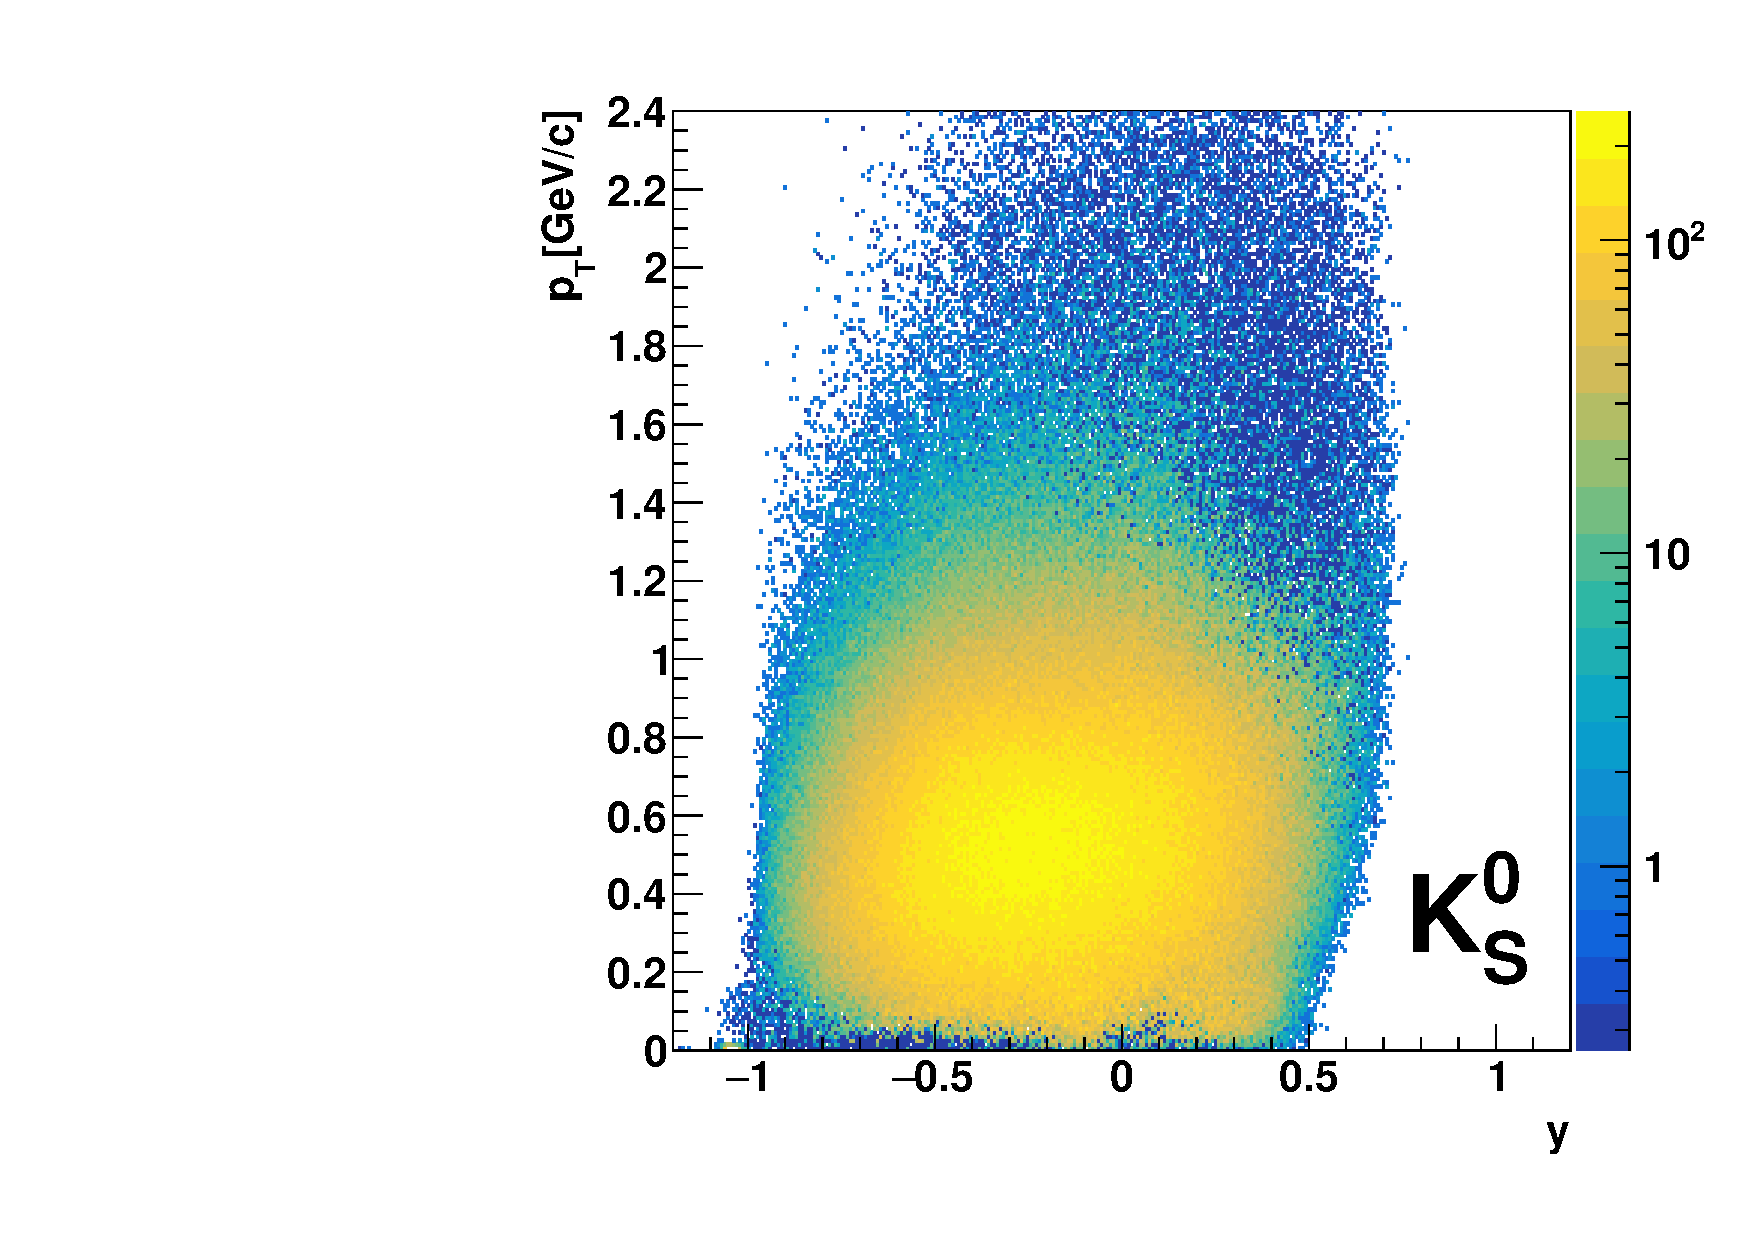
\includegraphics[width=0.49\linewidth]{chapterX/fig/ks_acceptance_v15.pdf}
%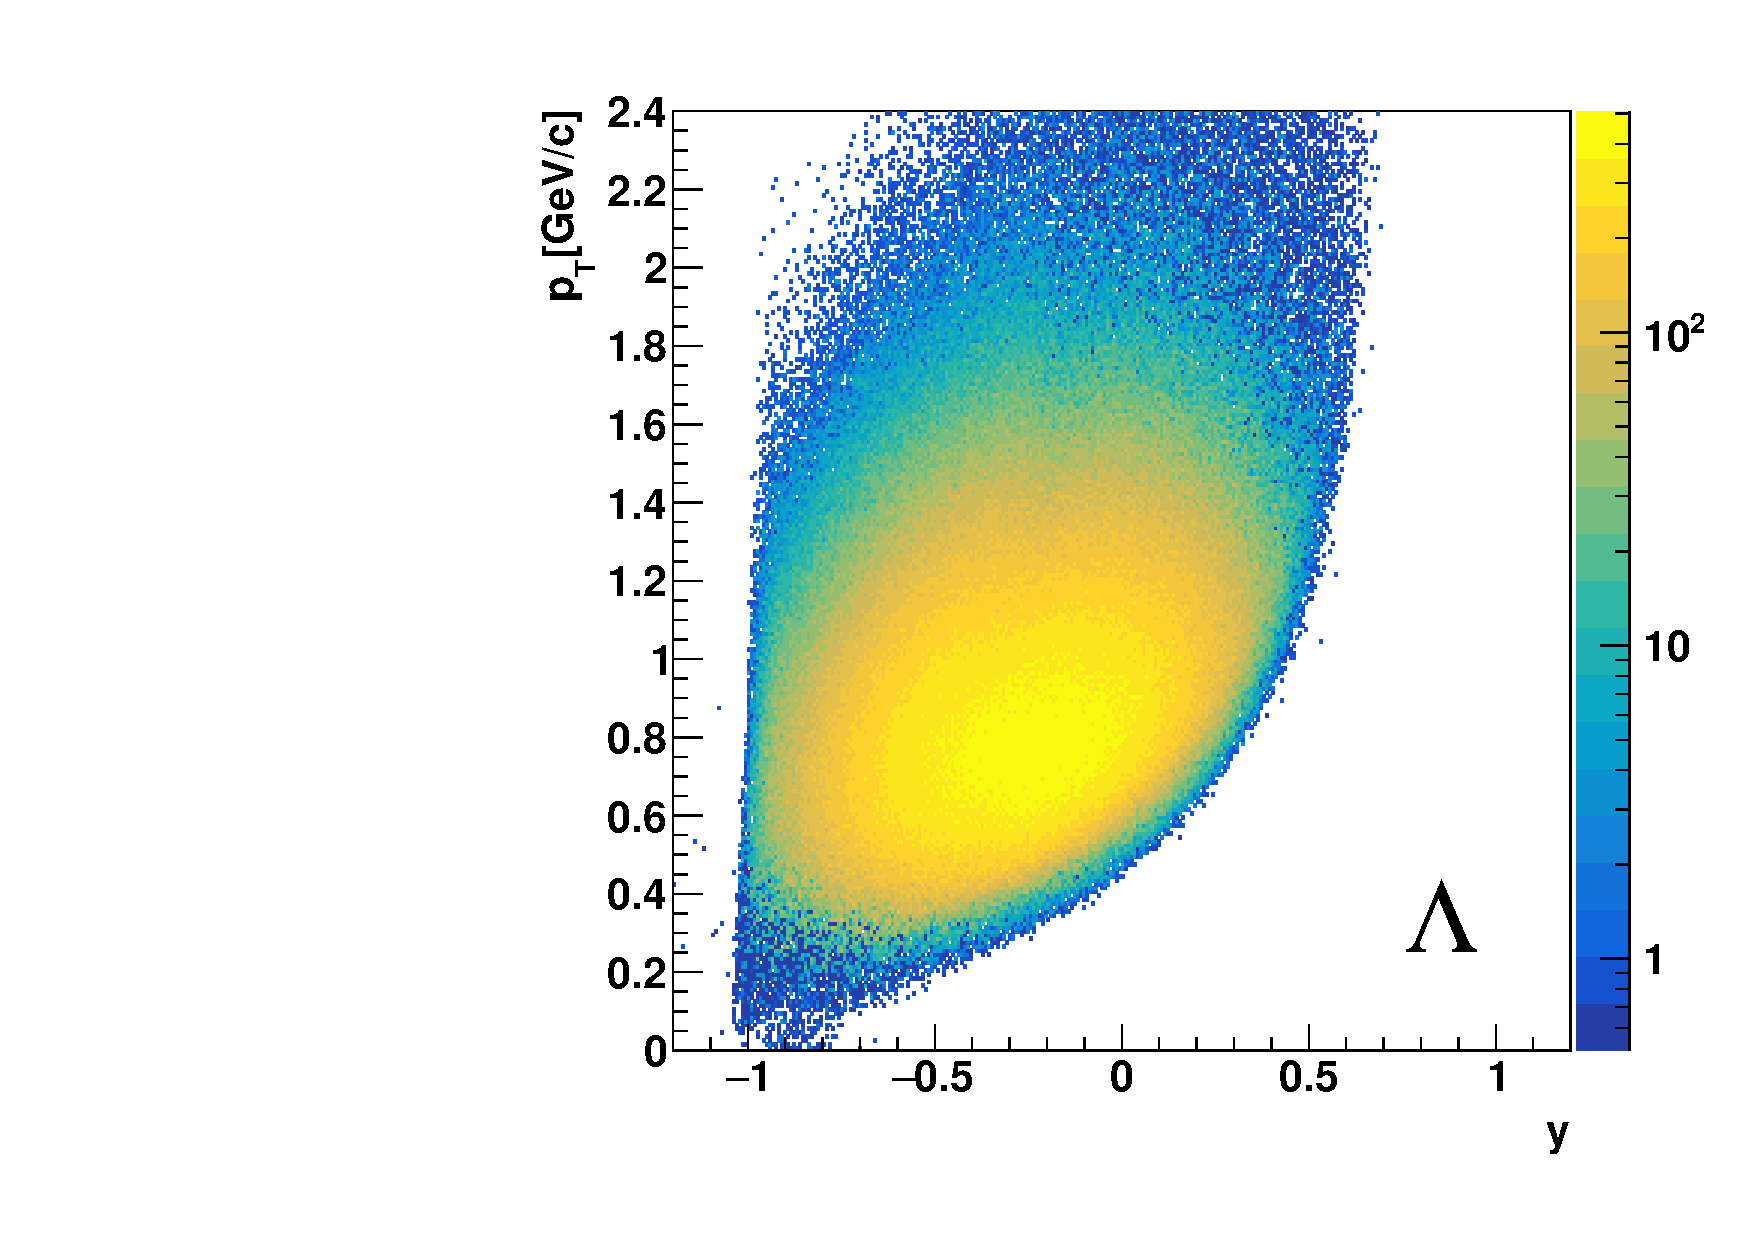
\includegraphics[width=0.49\linewidth]{chapterX/fig/ld_acceptance_v15.pdf}
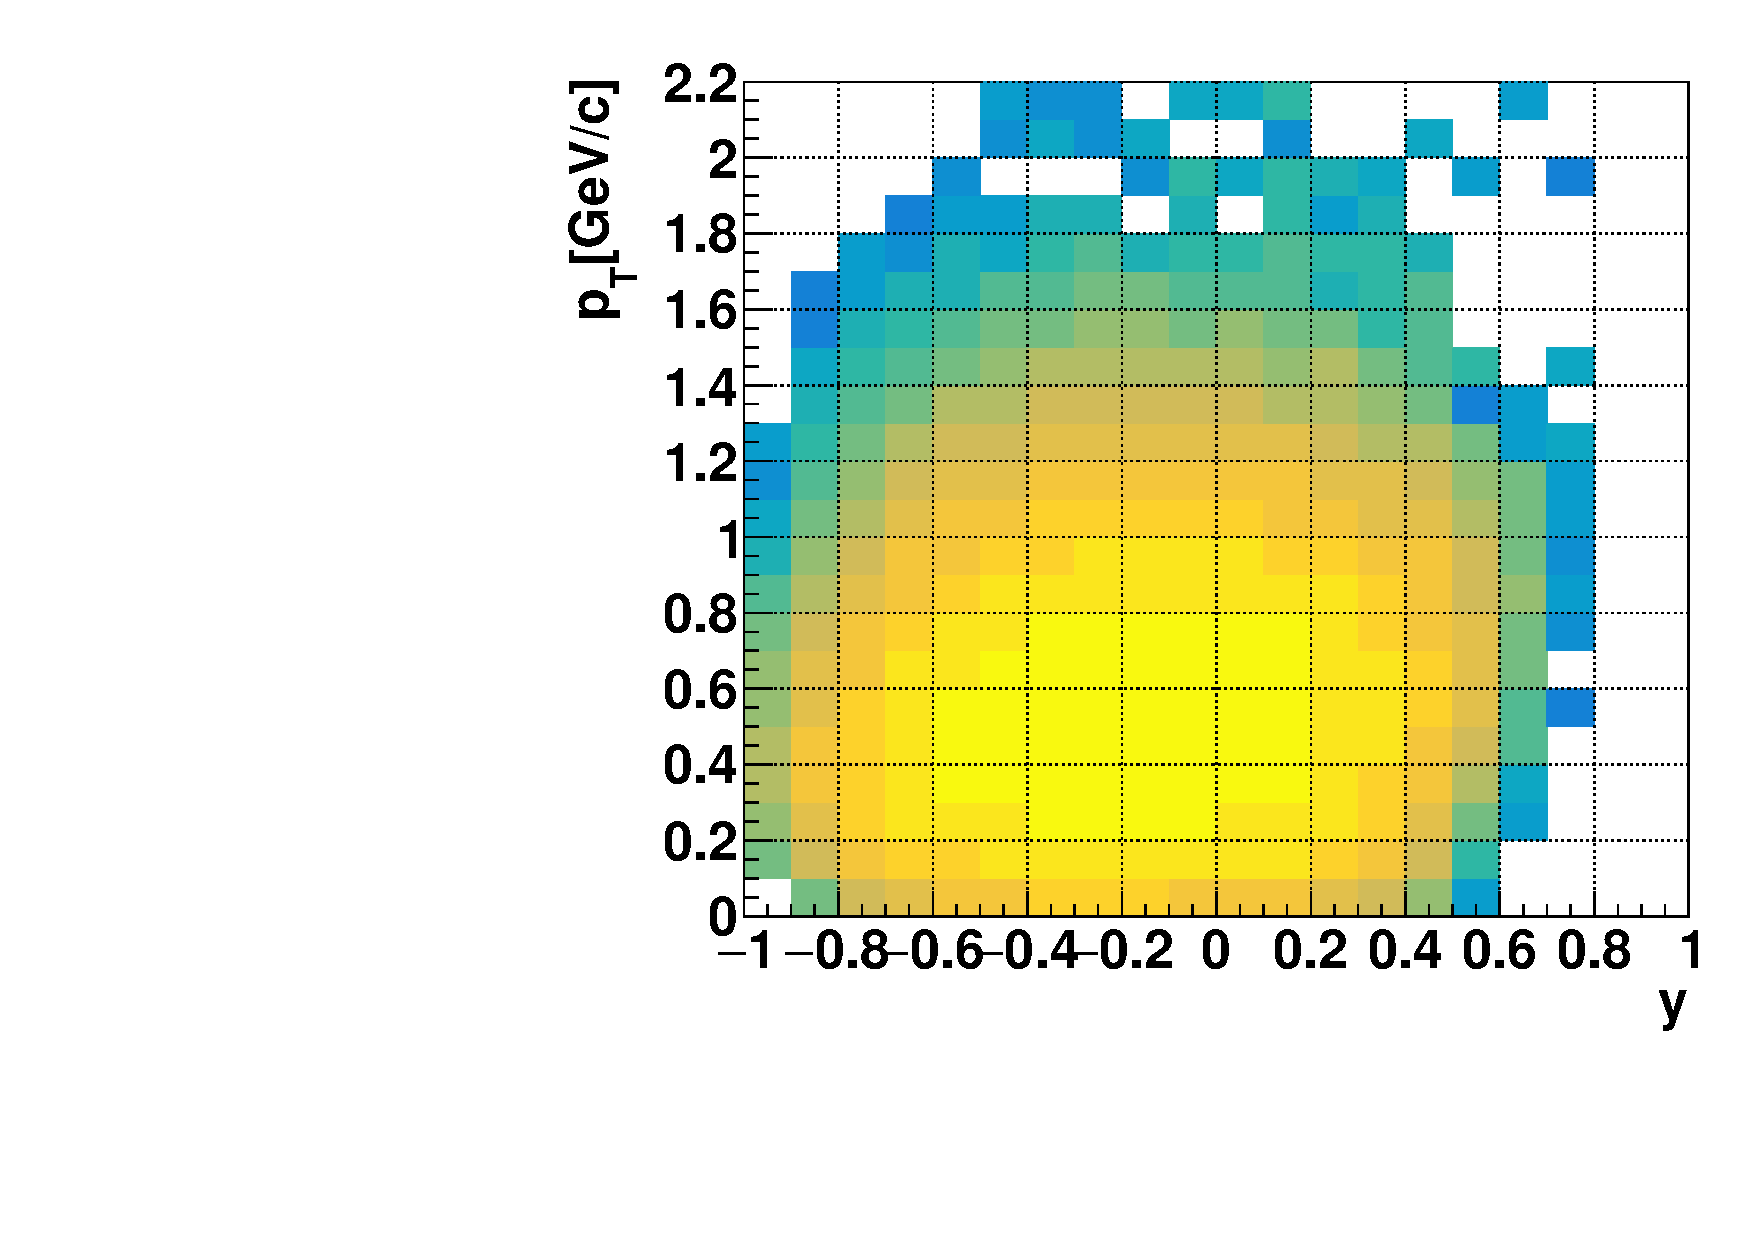
\includegraphics[width=0.49\linewidth]{chapterX/fig/ks_acc_v17.pdf}
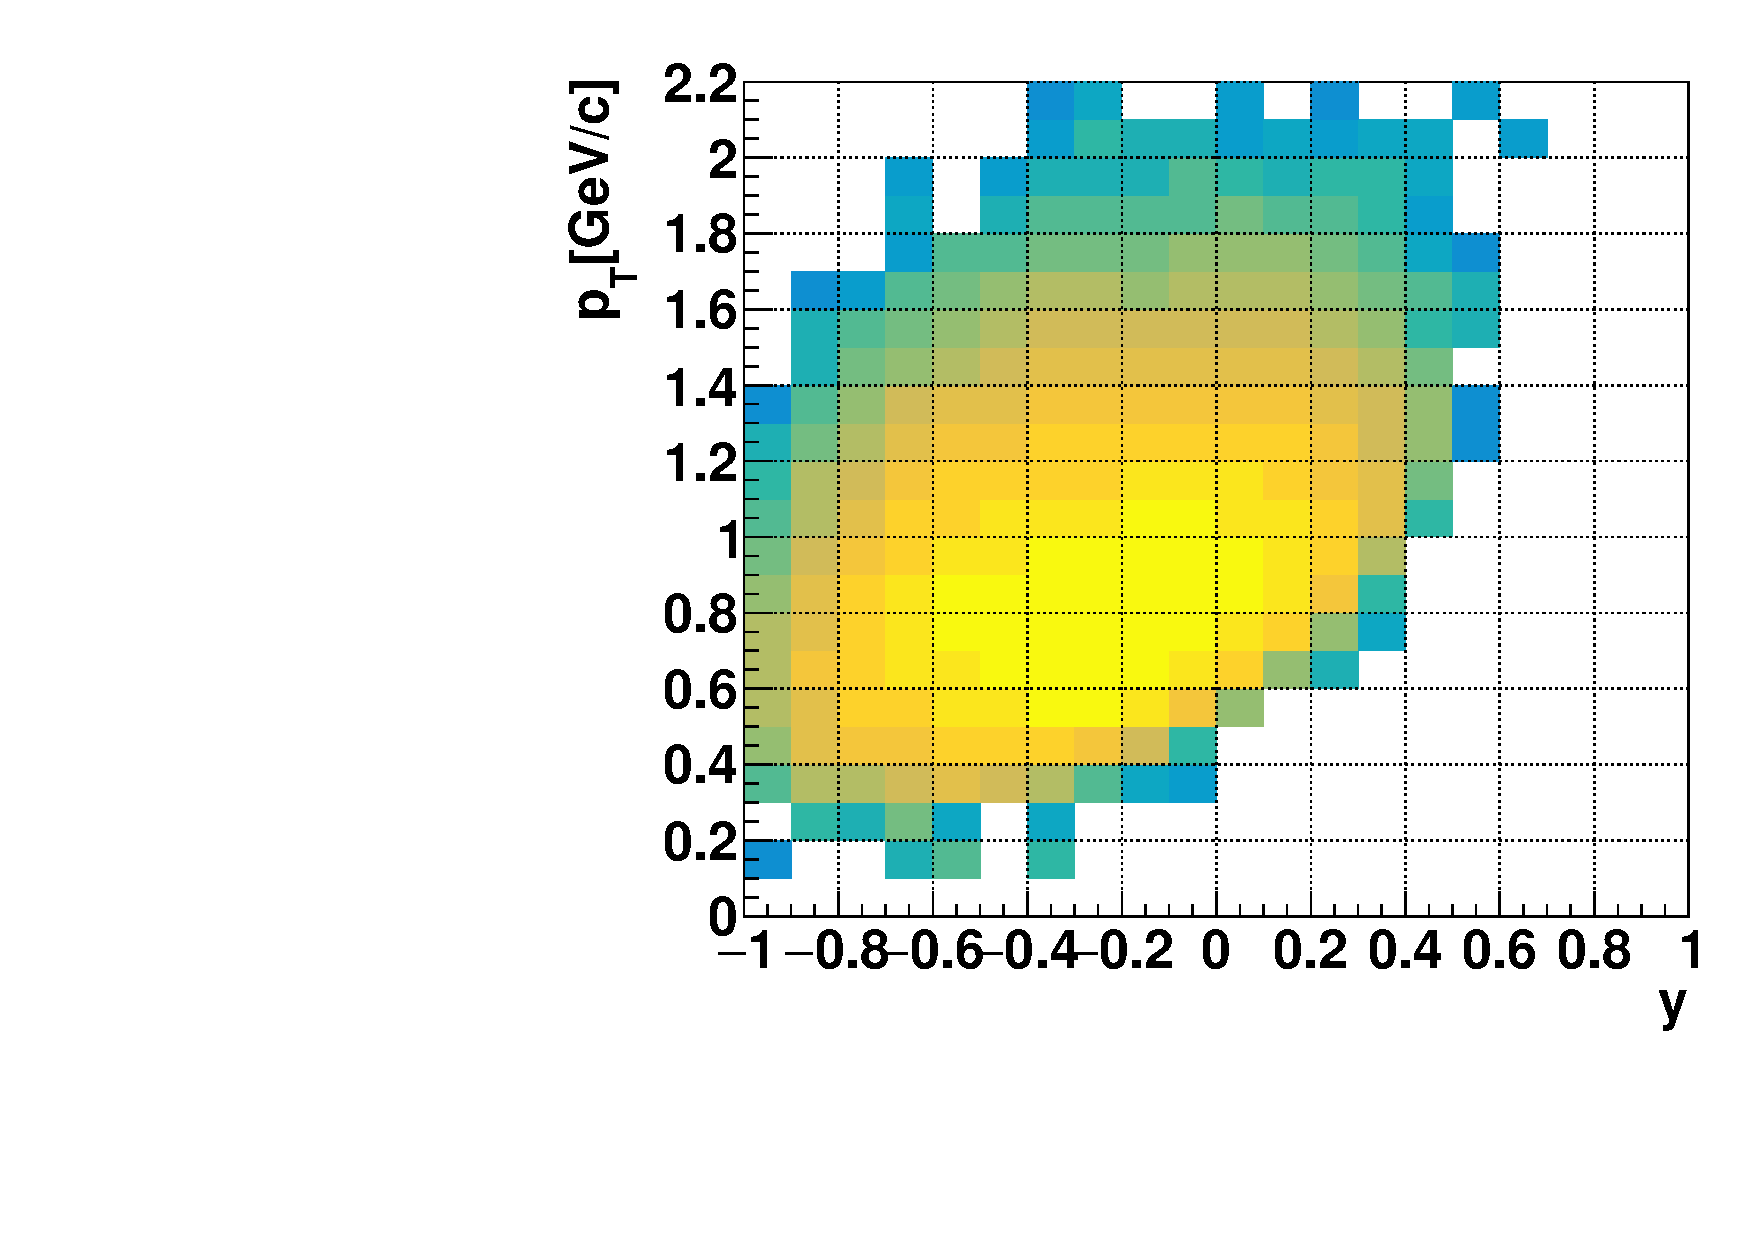
\includegraphics[width=0.49\linewidth]{chapterX/fig/ld_acc_v17.pdf}
\caption{Acceptance of $K^0_S$(left) and $\Lambda$(right) for $10-40\%$ centrality at $\sqrt{s_{NN}}$ = 3 GeV.}
\label{ldks_acceptance}
\end{figure}

We can extract the number of $K^0_S$ and $\Lambda$ using a simple bin counting method. This will be elaborated in more detail in later sections. Fig.~\ref{ldks_acceptance} shows schematically the number of counts as a function of rapidity and transverse momentum. For $v_{n}$ analysis, we choose the kinematic region $-1<y<0.5$ and $0.2<p_{T}<2$[GeV/$c$] for $K^0_S$, and $-1<y<0$ and $0.4<p_{T}<2$[GeV/$c$] for $\Lambda$. 


\subsubsection{Efficiency corrections}

\begin{figure}[h]
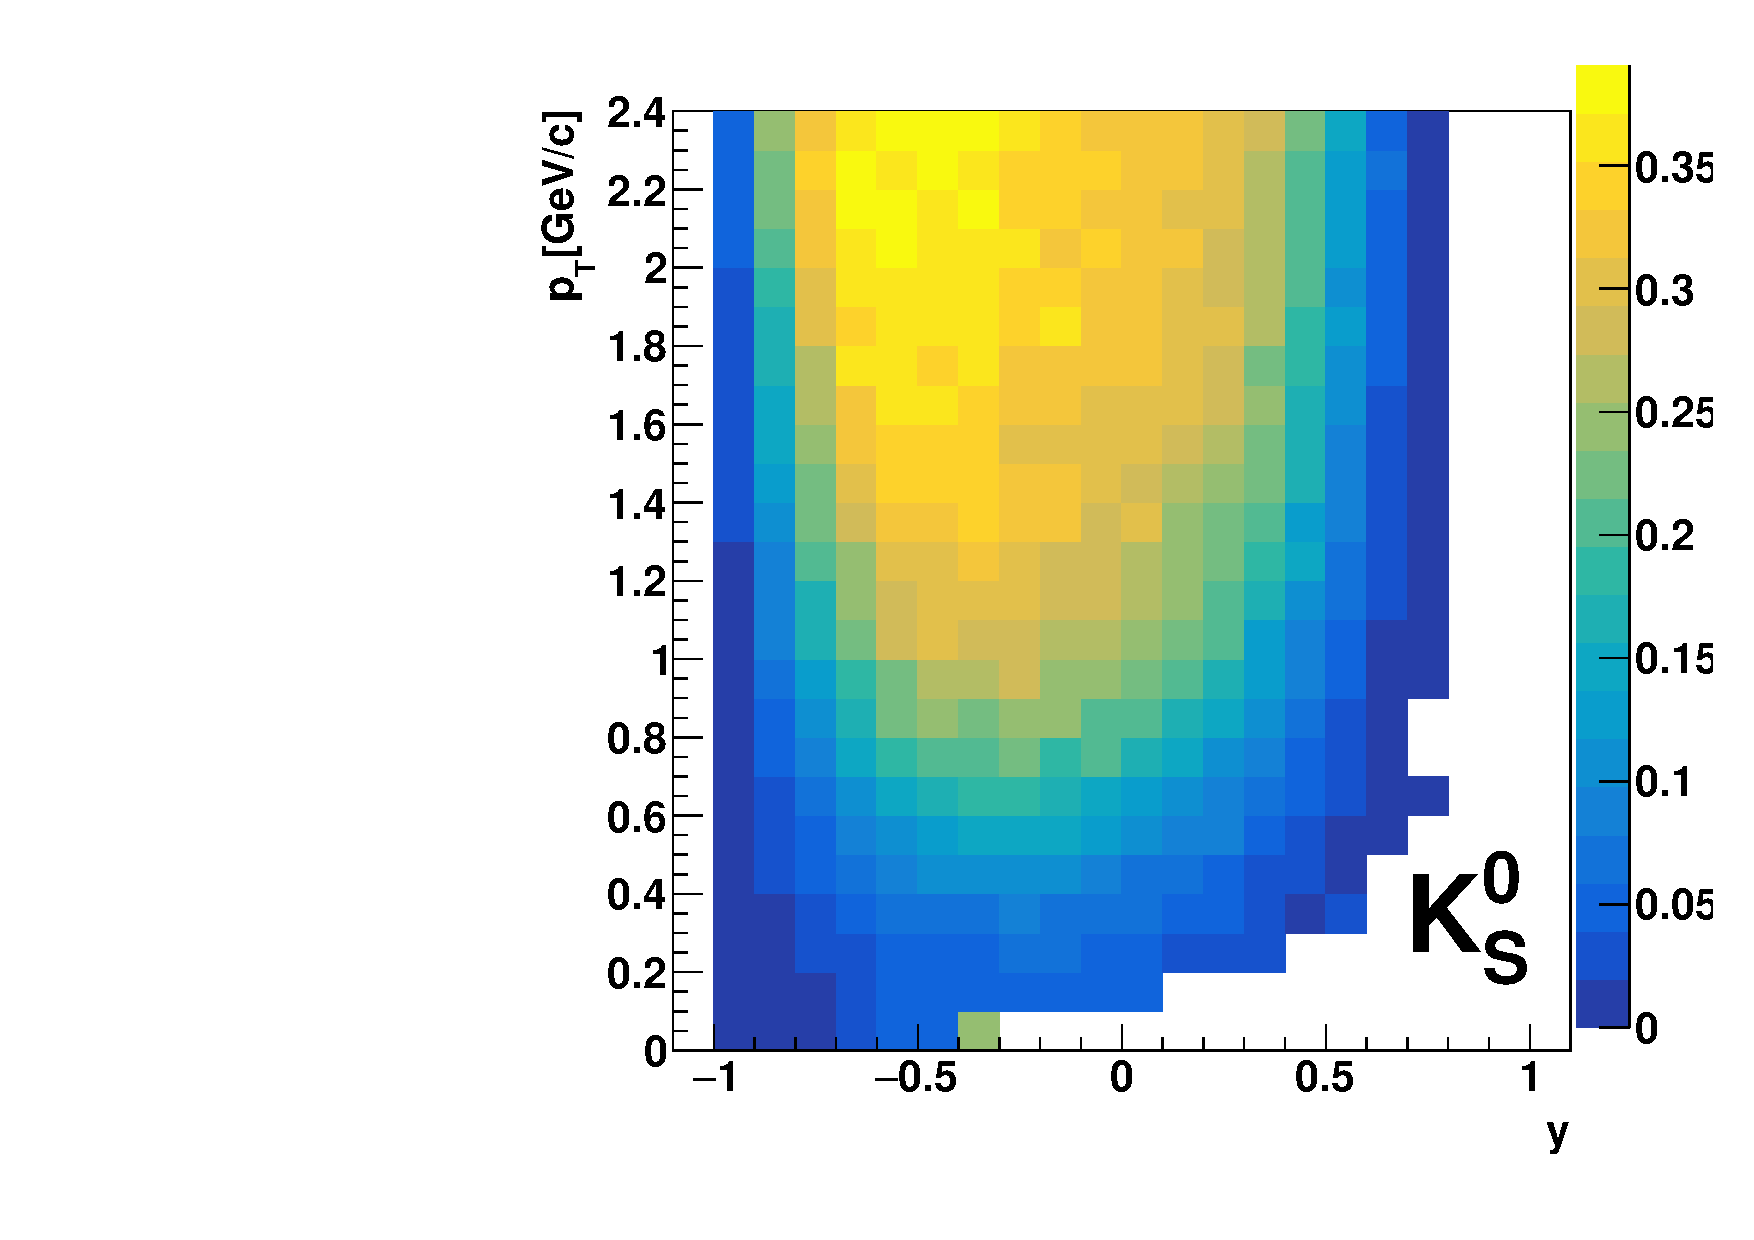
\includegraphics[width=0.49\linewidth]{chapterX/fig/ks_efficiency_v15.pdf}
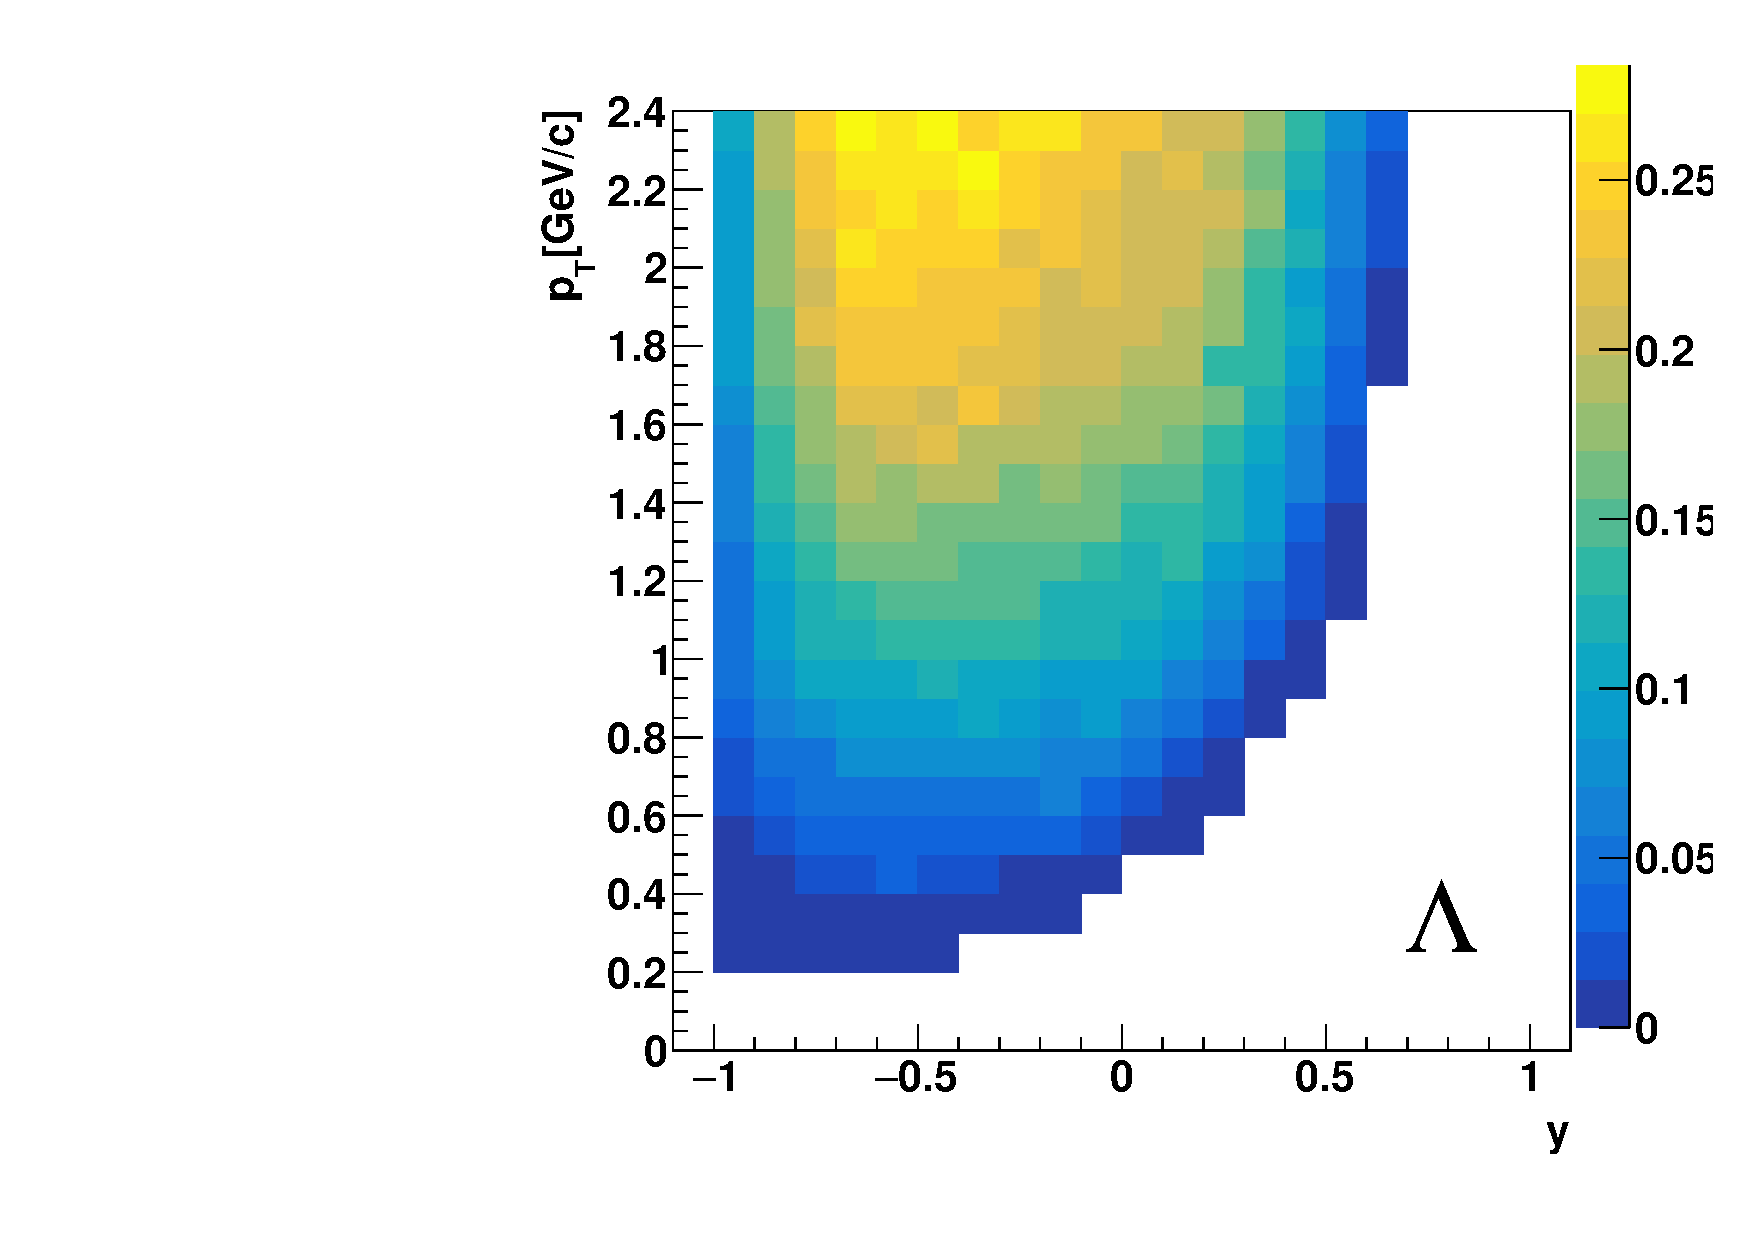
\includegraphics[width=0.49\linewidth]{chapterX/fig/ld_efficiency_v15.pdf}
\caption{Reconstruction efficiency of $K^0_S$(left) and $\Lambda$(right), as a function of $y$ and $p_{\rm{T}}$ for $10-40\%$ centrality at $\sqrt{s_{NN}}$ = 3 GeV.}
\label{ldks_eff}
\end{figure}

The kinematic regions listed in the previous section does not have uniform efficiency, hence we need to apply efficiency correction in order to obtain $v_n$. To calculate the efficiency, we reconstruct $K^0_S$ and $\Lambda$ from embedding samples. The efficiency is obtained by dividing the number of reconstructed 
$K^0_S$ or $\Lambda$, by the number of input $K^0_S$ or $\Lambda$, for each $y$ and $p_{T}$ bin. The track and topological cuts used are identical to the ones used in the data analysis, i.e. the cuts listed in Tab.~\ref{tab:kfptcldkscuts}. The 2D efficiency is shown in Fig.~\ref{ldks_eff}. 

To ensure the efficiency obtained is reliable, we compare the topological variables from data, and embedding. It was confirmed that the topological variables can be reasonably described by the embedding~\url{(https://drupal.star.bnl.gov/STAR/system/files/lfsupc20200607\_0.pdf)}. The cuts used will be varied as an estimate of the systematic uncertainties associated to efficiency corrections.


\subsection{$v_1$ and $v_2$ extraction}
We use the KFParticle package to reconstruct $K^0_S$ and $\Lambda$. After that, we fill 3D histograms in $y$, $p_{T}$, and $\phi-\Psi_{N}$. Each entry is weighted, by the inverse of the 2D efficiency (as a function of $y$ and $p_{T}$, shown in Fig.~\ref{ldks_eff}. In addition, it is weighted by the inverse of the resolution~\ref{https://arxiv.org/pdf/1212.3650.pdf}. This accounts for the fact that we are using wide centrality bins, i.e. $10-40\%$, and that there exist non-negligible variations in the resolution within the wide centrality bin. 

\subsubsection{$v_1$ extraction for $\Lambda$}

We extract $v_1$ for $10-40\%$, over the $p_{T}$ region $0.4-2.0$ [GeV/$c$], and $y=-1 --0$. 
The projections of the histograms for $10-40\%$ are shown in Fig.~\ref{ld_v1_sig_raw} and~\ref{ld_v1_sig_raw2}. To obtain the number of counts, we also generate background distributions, by rotating $\pi^{-}$ tracks by $\pi$. The background is normalized using the side band region. Both data and the background are shown in Fig.~\ref{ld_v1_sig} and~\ref{ld_v1_sig2}.

The background is subsequently subtracted from the data. One can see that for most of the phase space, the background is well described by the rotation method. In order to take account of any residual background, we fit the subtracted data, by a linear function. The fit region is $5\sigma<|m-m_{PDG}|<10\sigma$. The fitted function is indicated as the black dotted line in Fig.~\ref{ld_v1_sig}. The bin counting method is used to extract the number of counts. The counting window is $|m-m_{PDG}|<3\sigma$, and is indicated as the vertical black dotted lines in Fig.~\ref{ld_v1_sig}.


\begin{figure}[h]
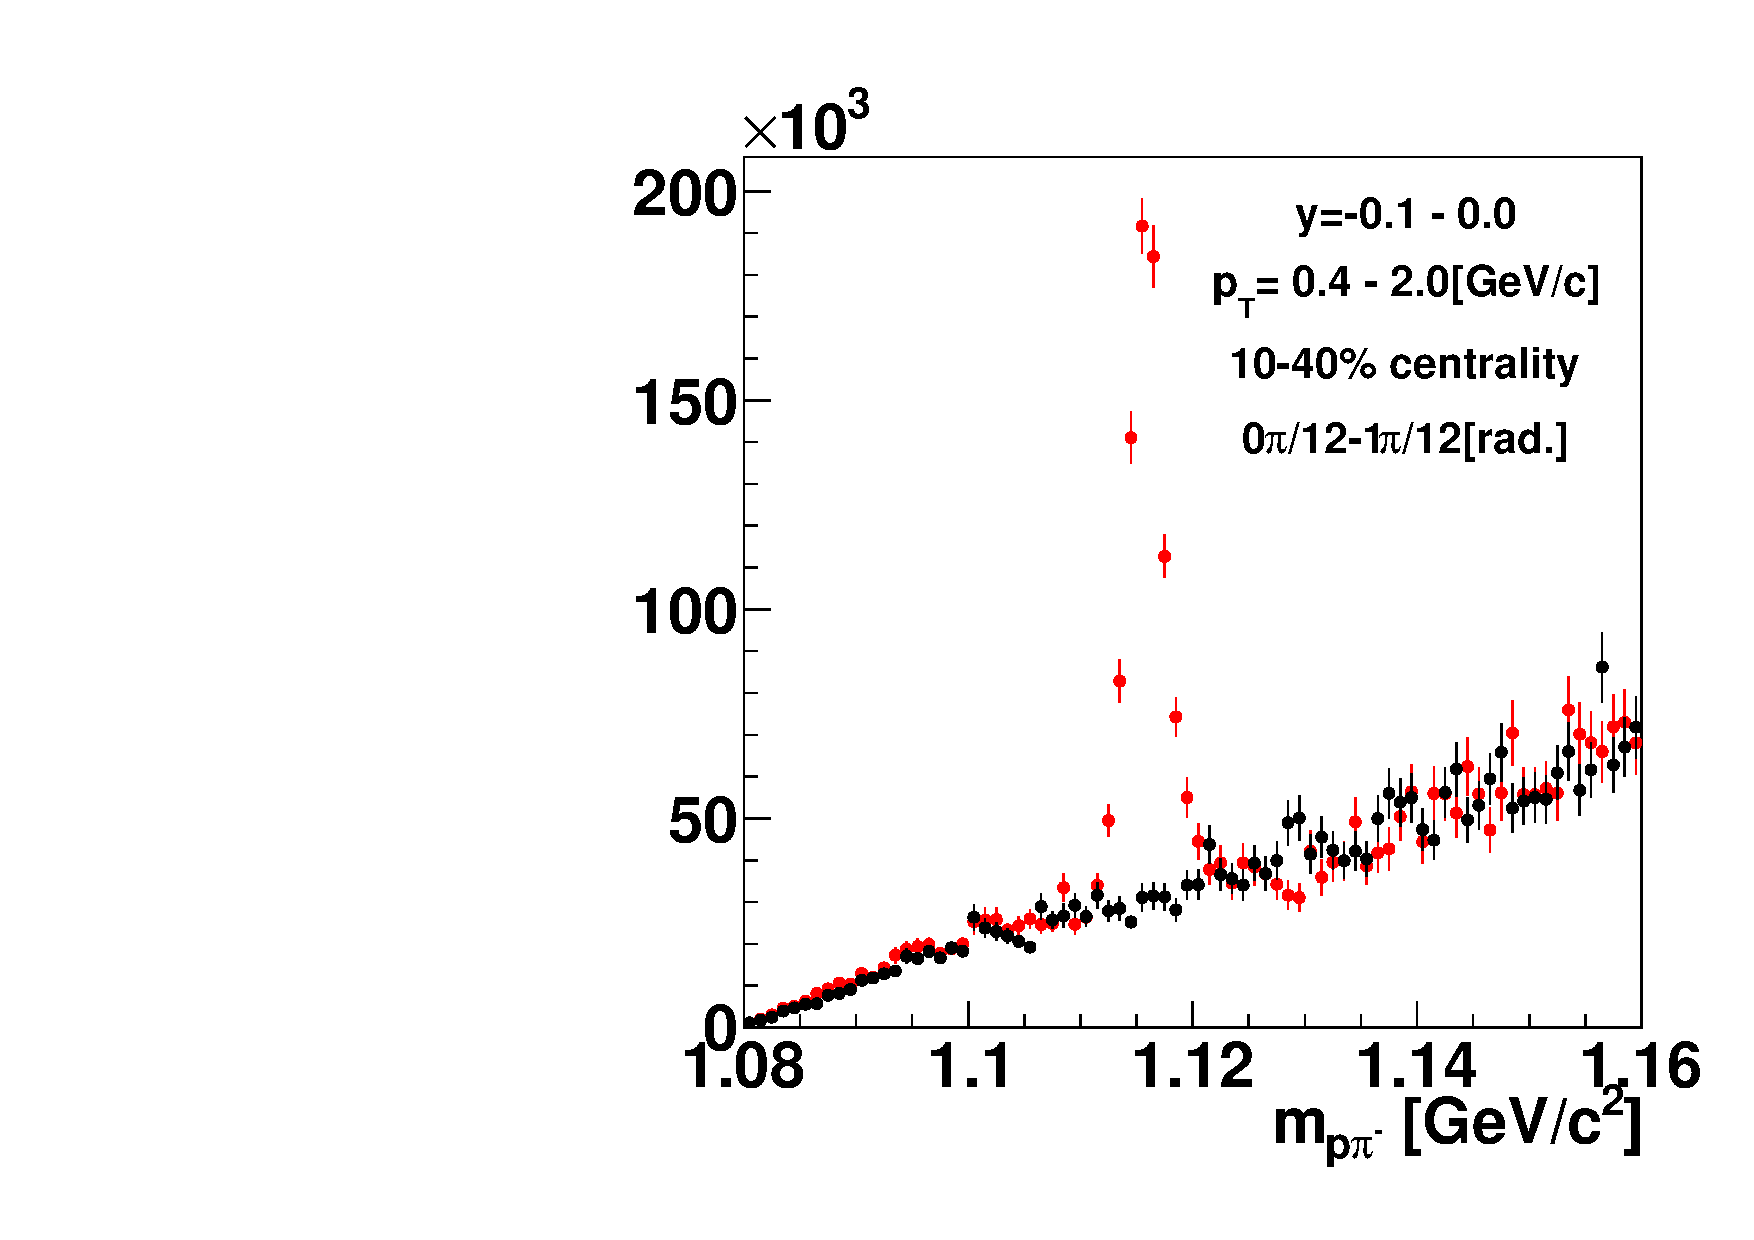
\includegraphics[width=0.14\linewidth]{chapterX/fig/ld_v1_sig/kf_ptslice0_cent1_ld_flow_phi1_rap5_check.pdf}
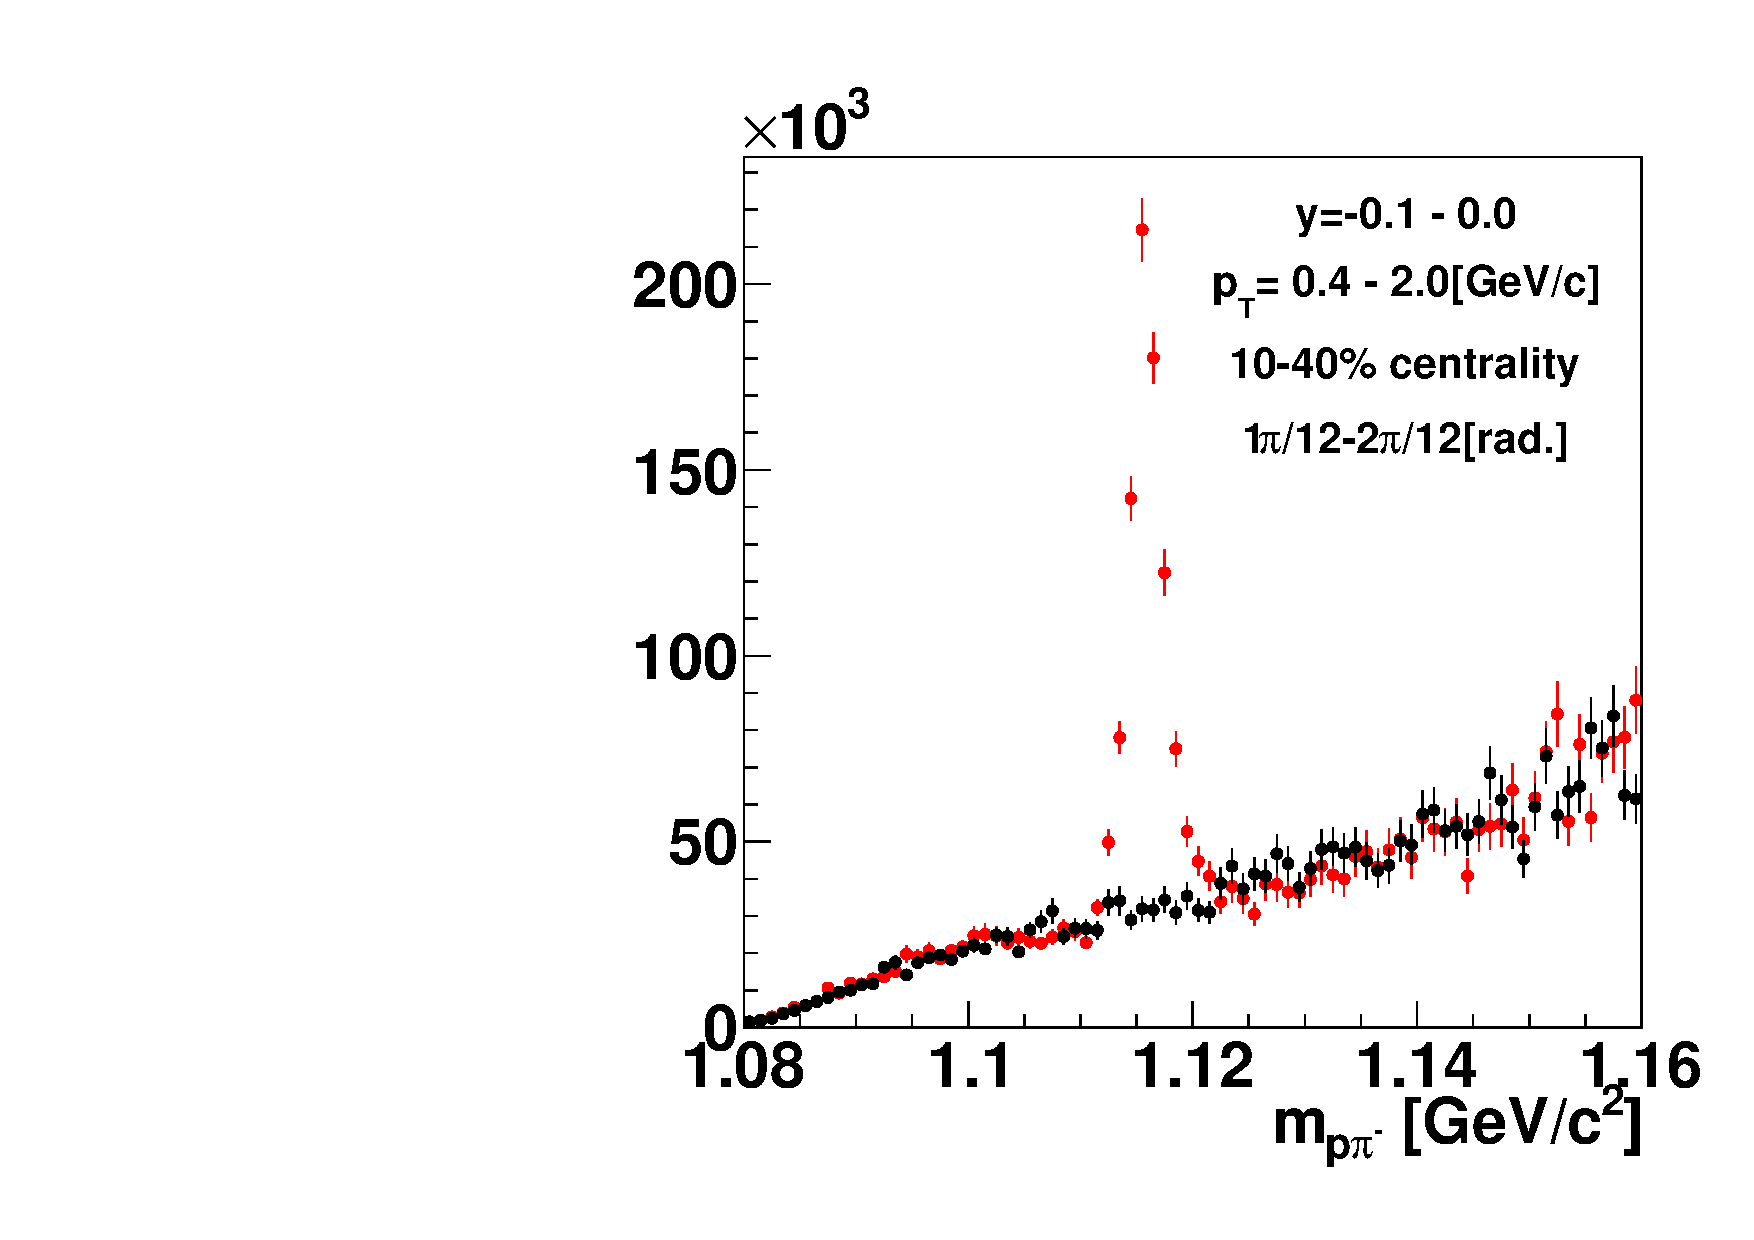
\includegraphics[width=0.14\linewidth]{chapterX/fig/ld_v1_sig/kf_ptslice0_cent1_ld_flow_phi2_rap5_check.pdf}
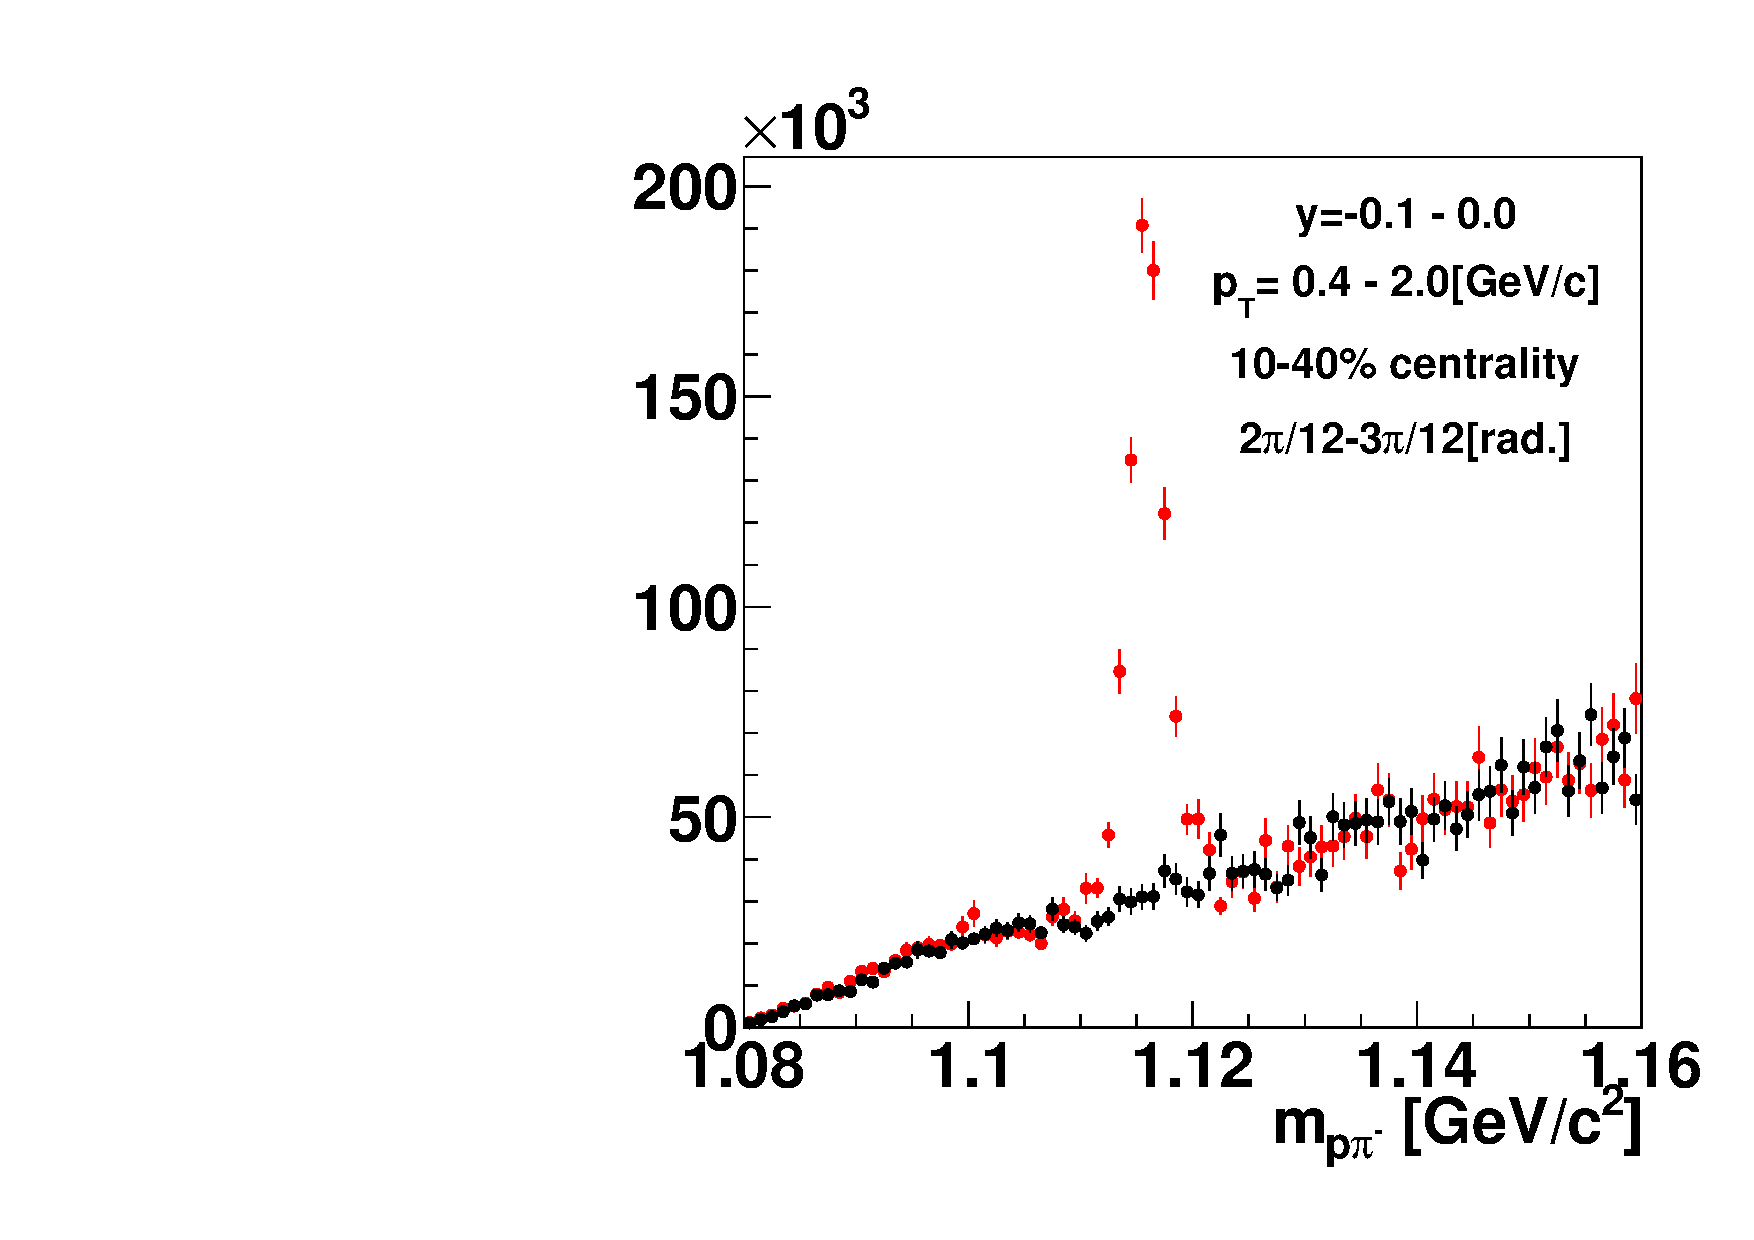
\includegraphics[width=0.14\linewidth]{chapterX/fig/ld_v1_sig/kf_ptslice0_cent1_ld_flow_phi3_rap5_check.pdf}
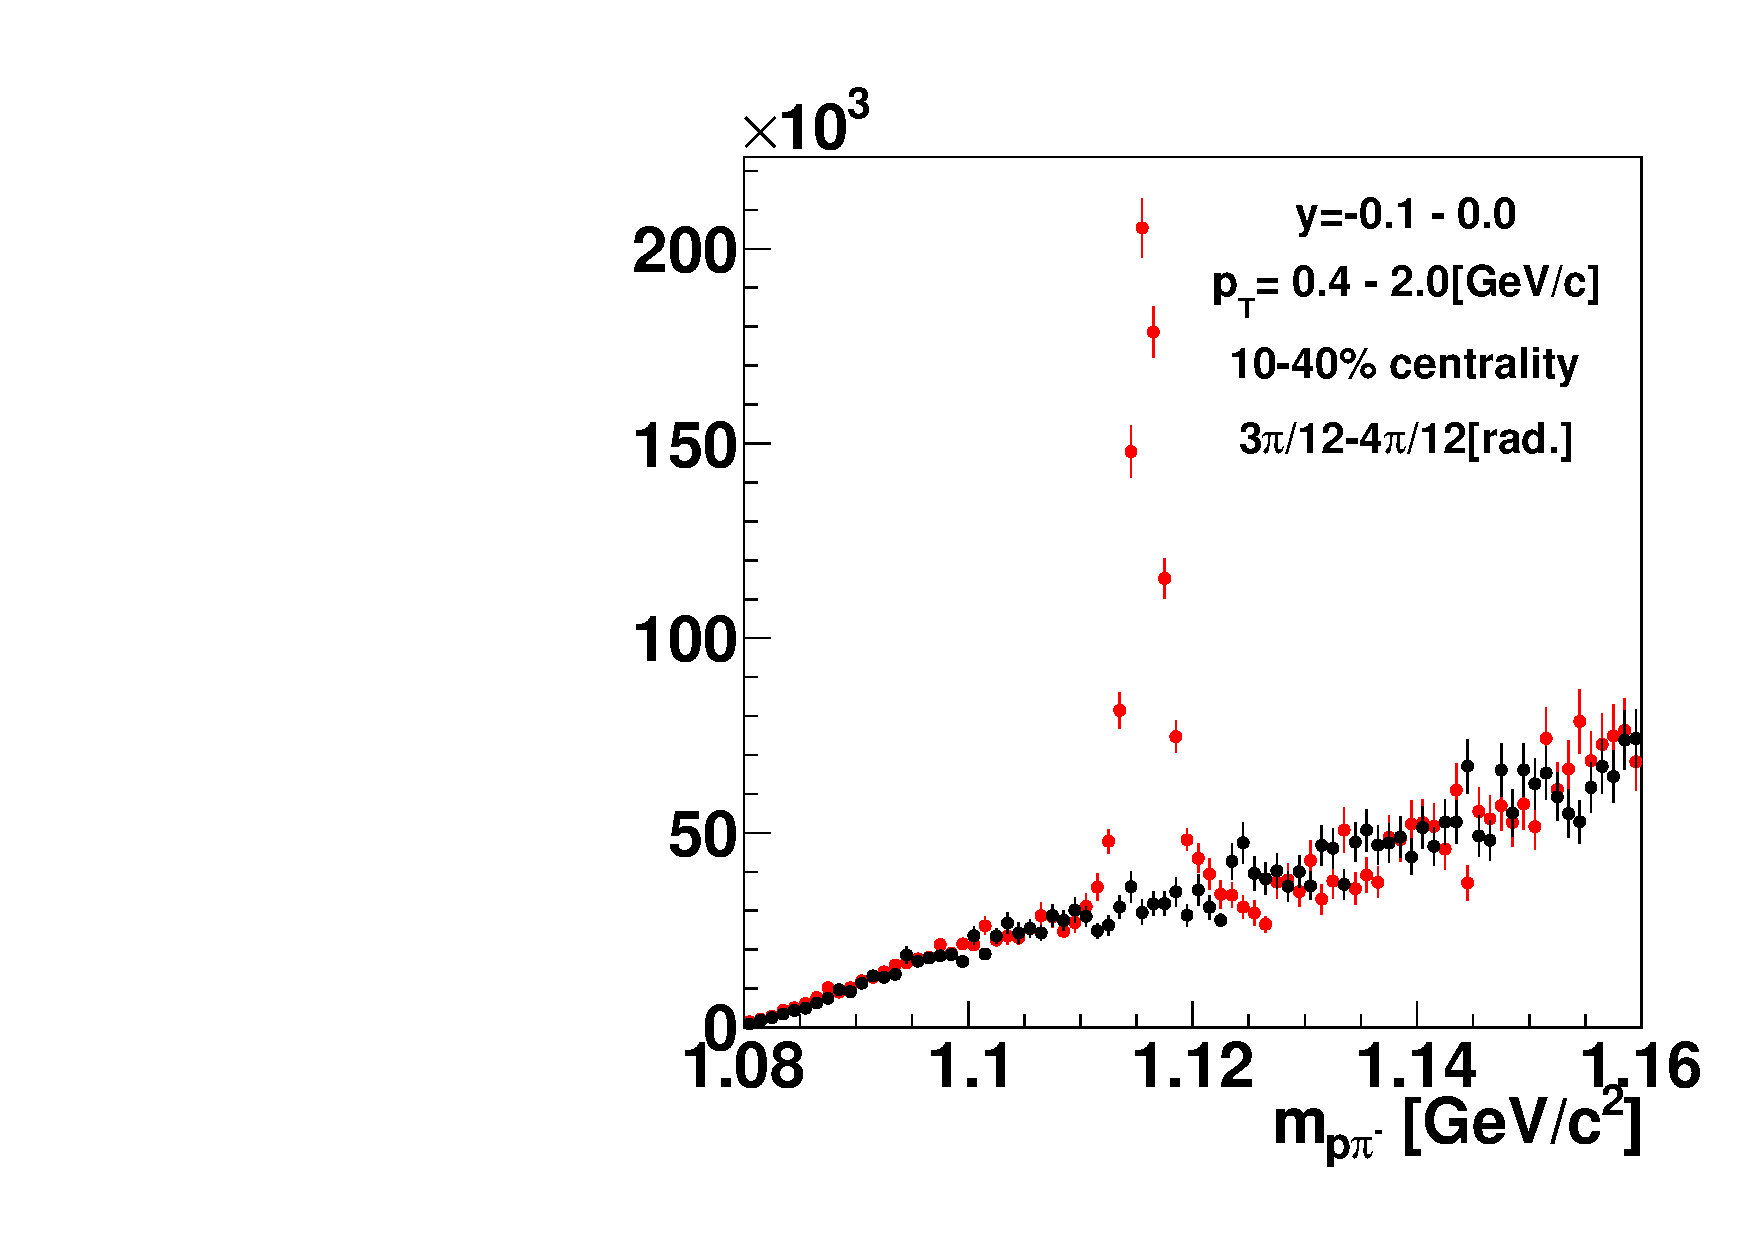
\includegraphics[width=0.14\linewidth]{chapterX/fig/ld_v1_sig/kf_ptslice0_cent1_ld_flow_phi4_rap5_check.pdf}
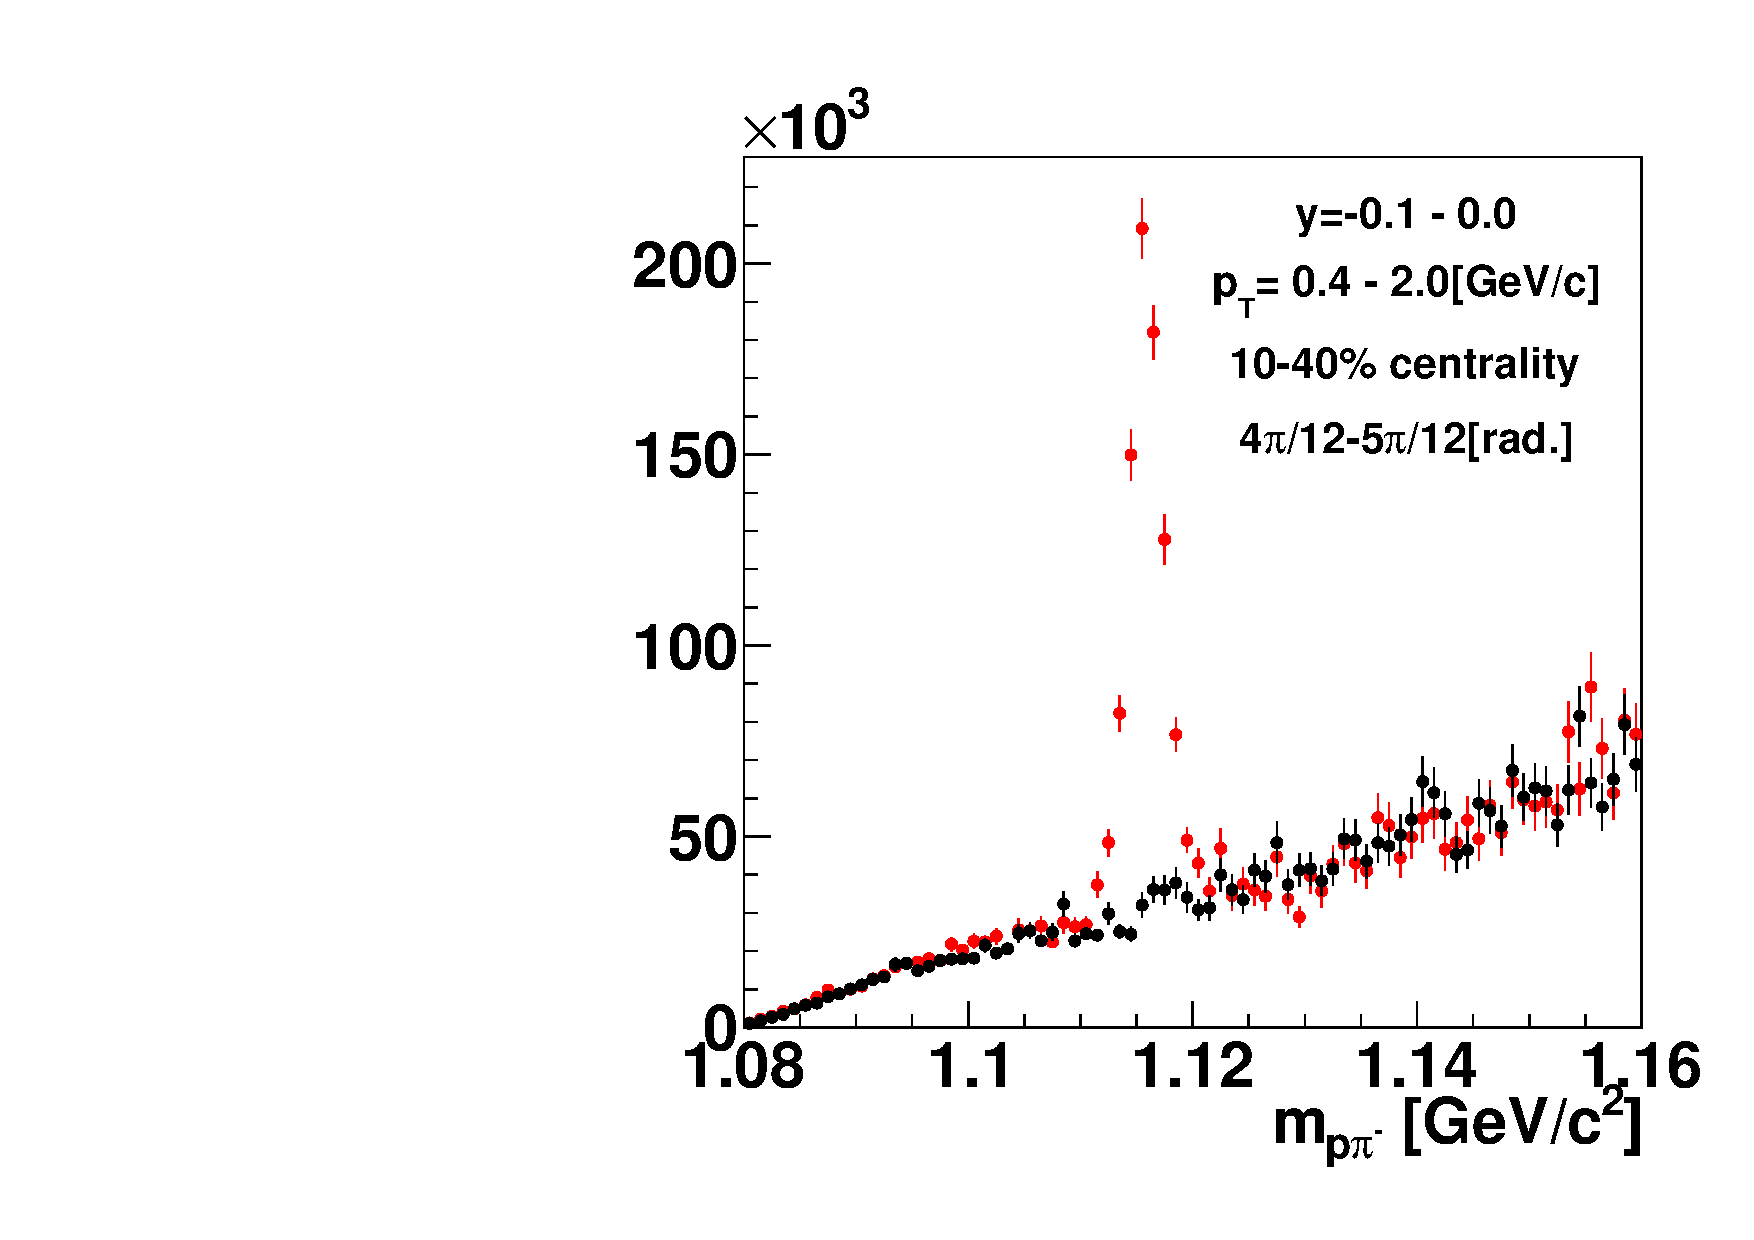
\includegraphics[width=0.14\linewidth]{chapterX/fig/ld_v1_sig/kf_ptslice0_cent1_ld_flow_phi5_rap5_check.pdf}
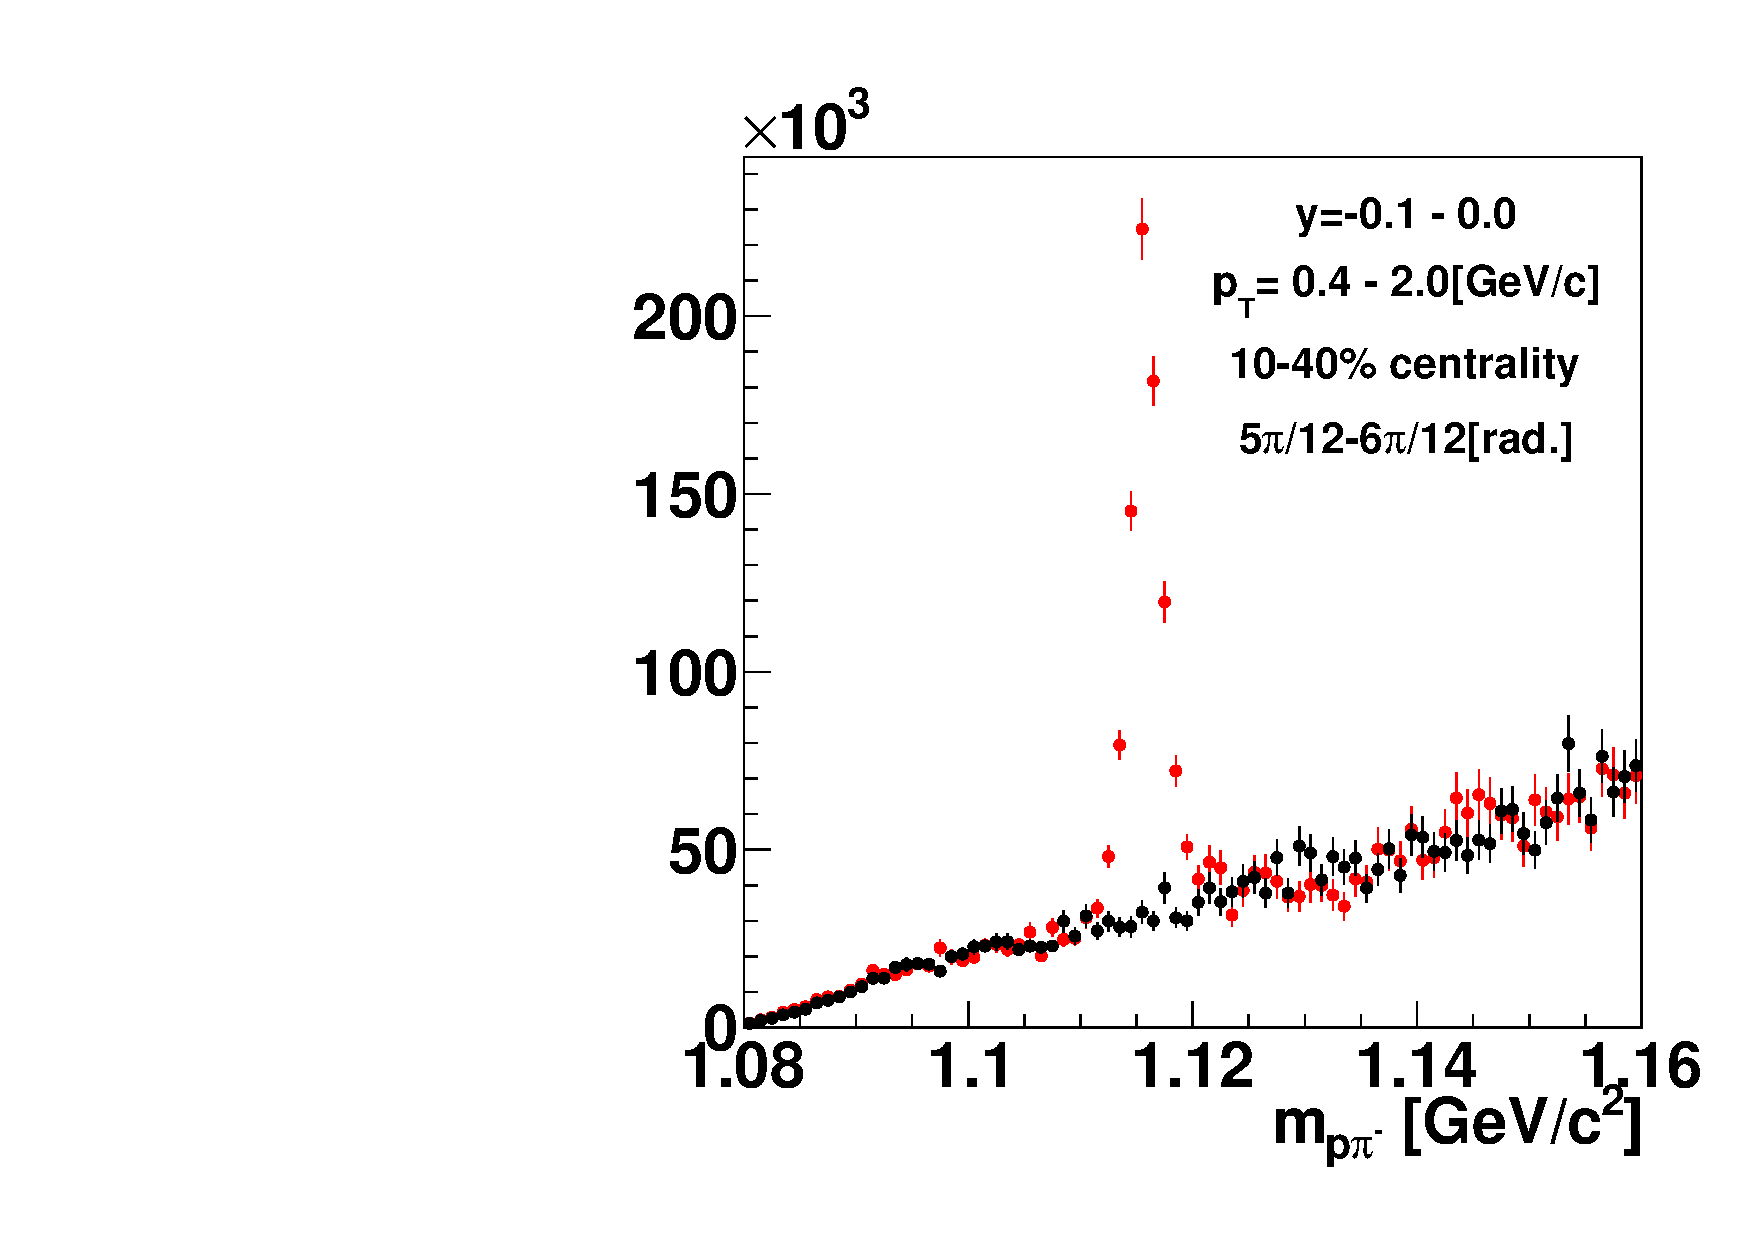
\includegraphics[width=0.14\linewidth]{chapterX/fig/ld_v1_sig/kf_ptslice0_cent1_ld_flow_phi6_rap5_check.pdf}
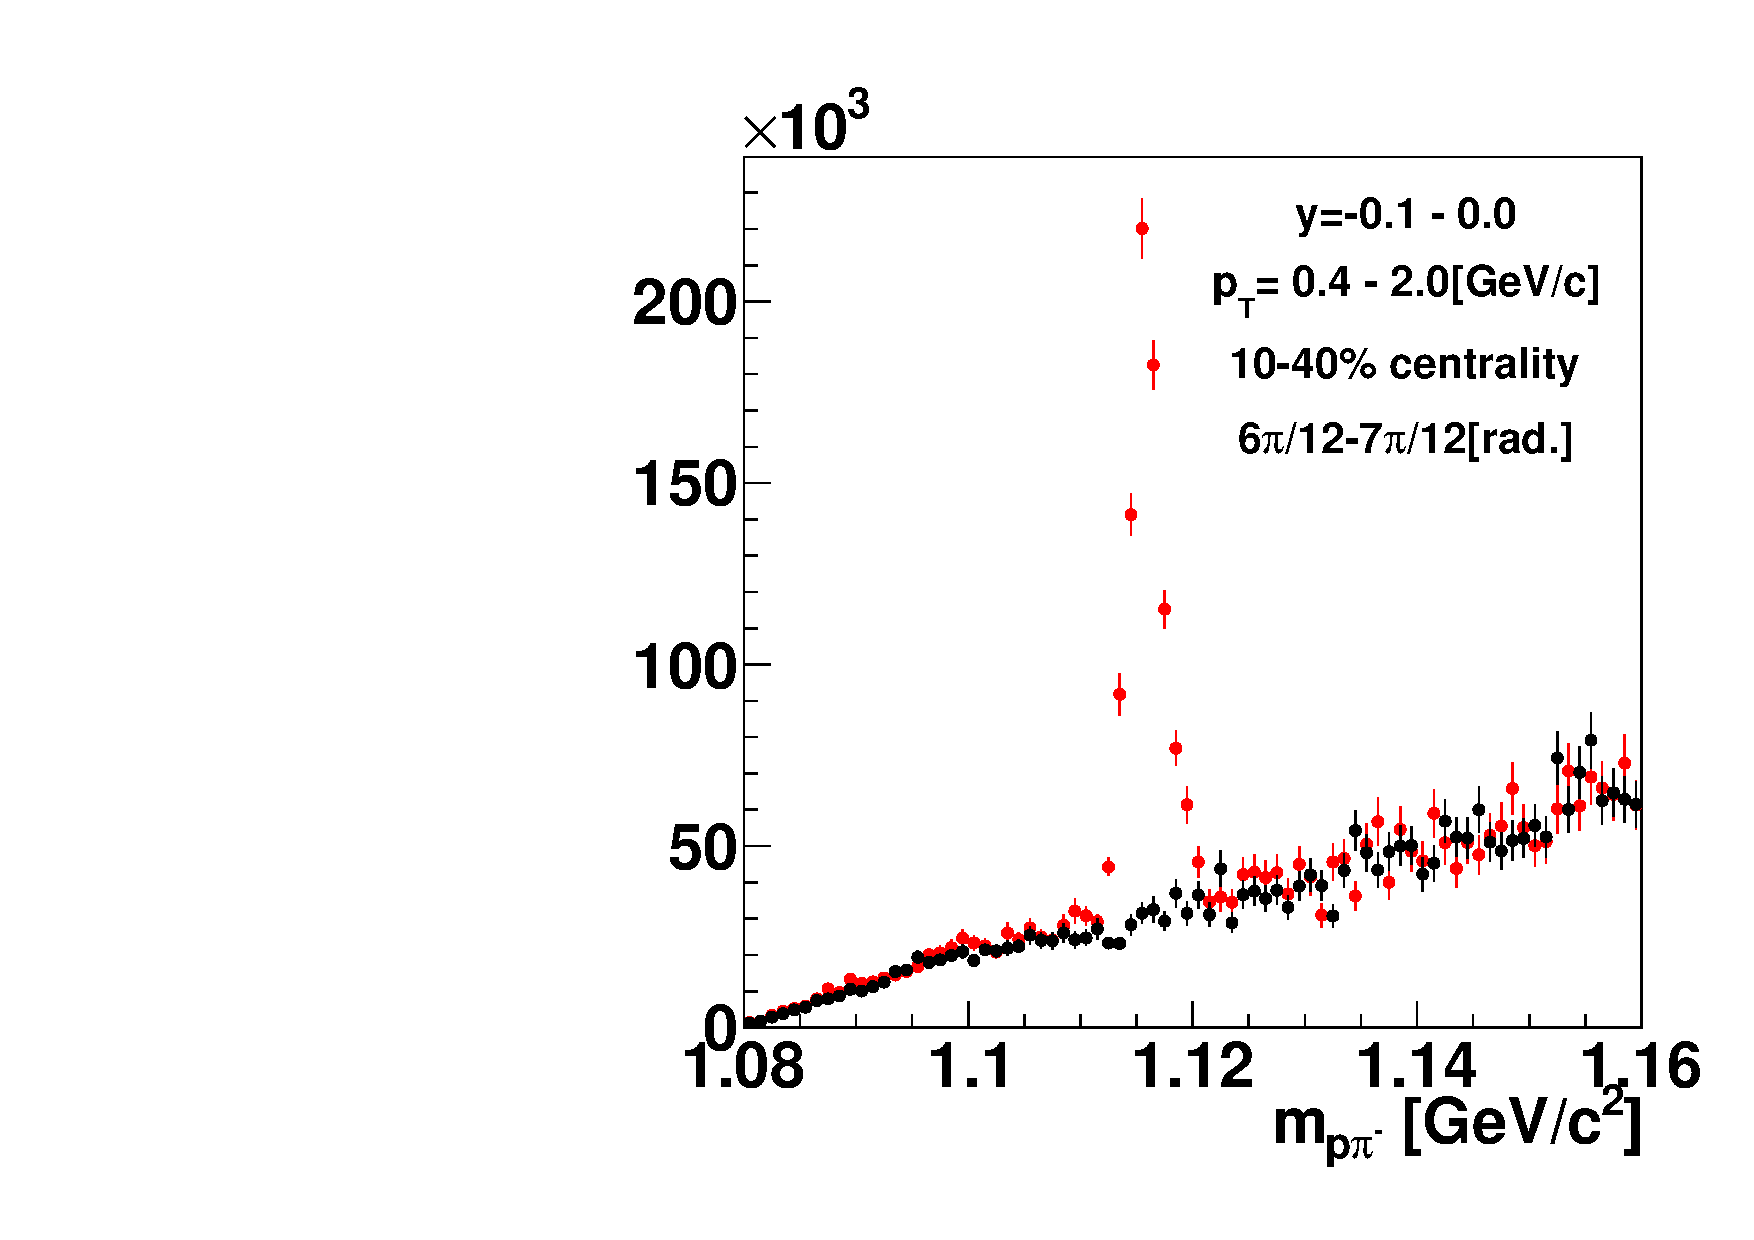
\includegraphics[width=0.14\linewidth]{chapterX/fig/ld_v1_sig/kf_ptslice0_cent1_ld_flow_phi7_rap5_check.pdf}
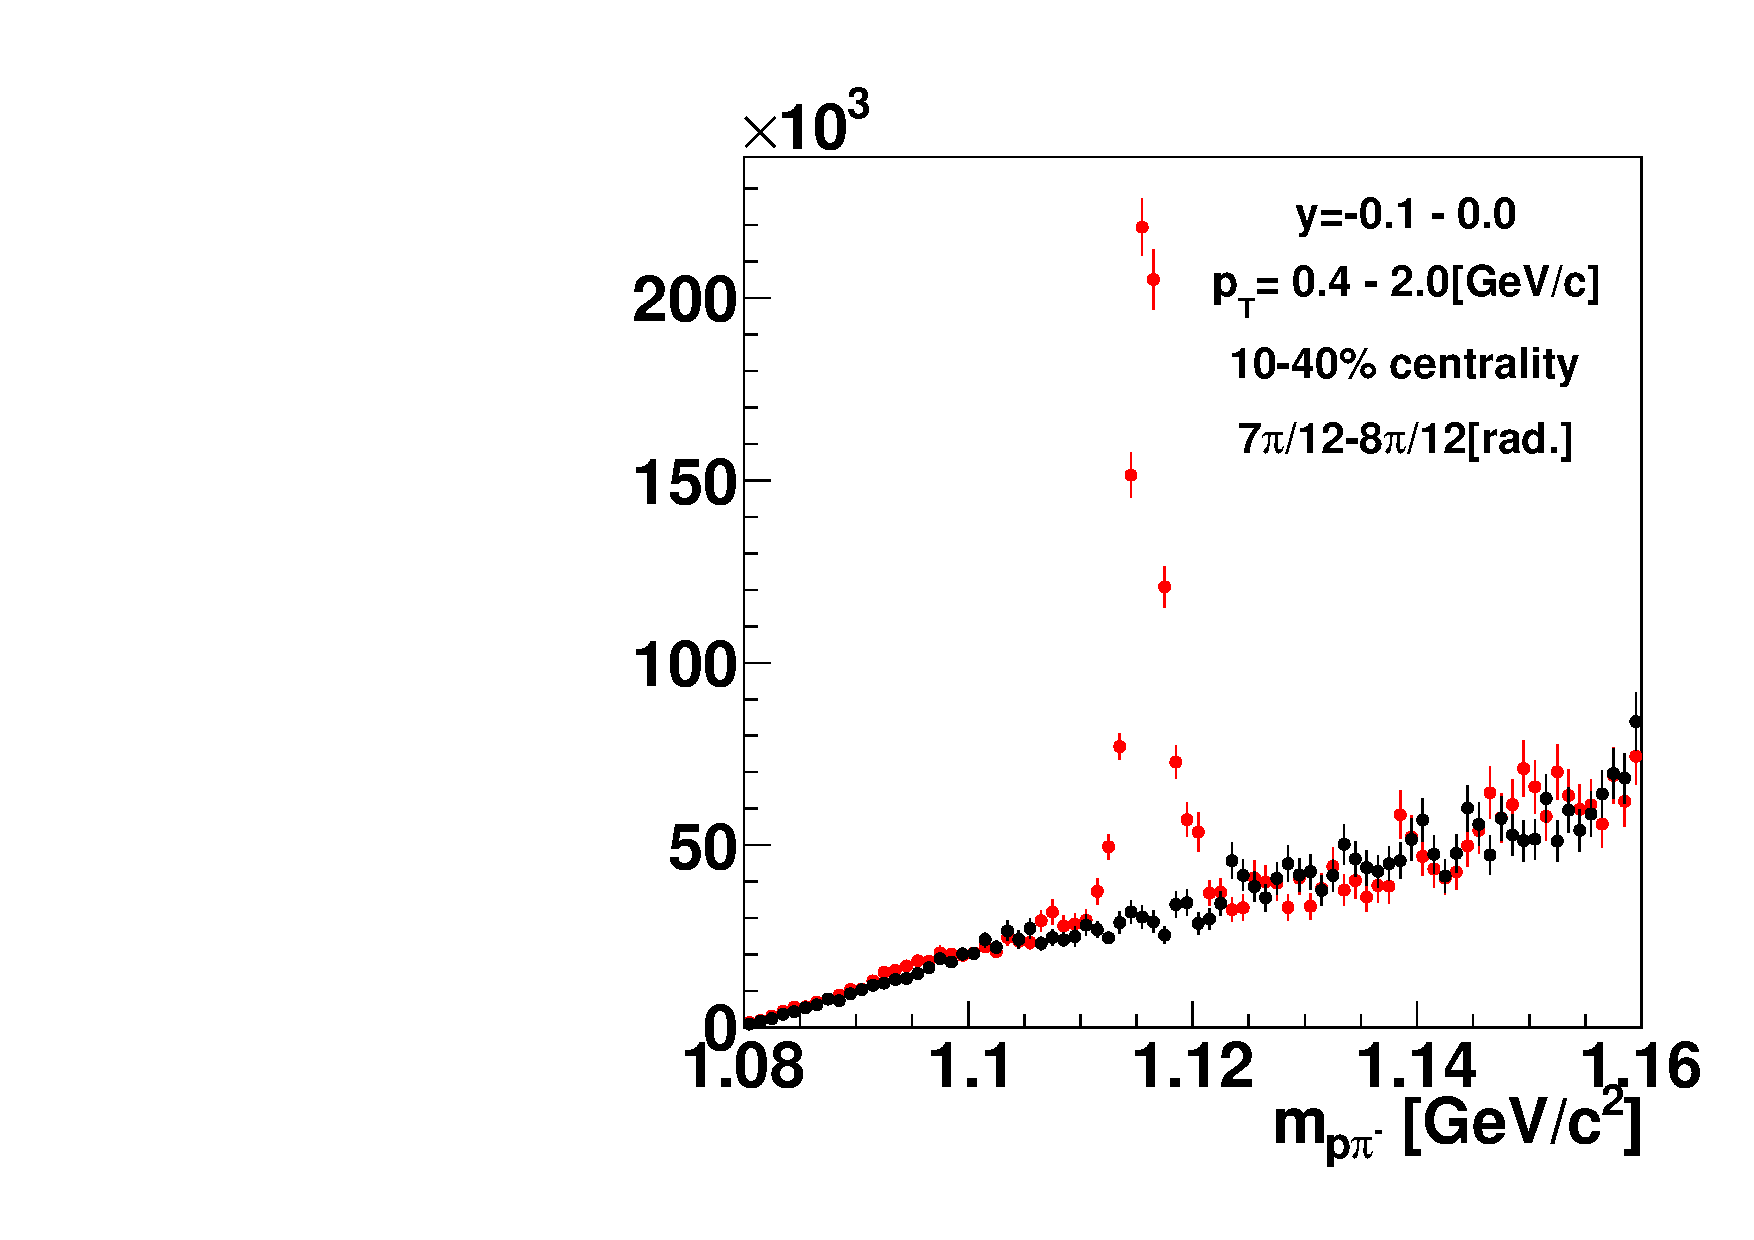
\includegraphics[width=0.14\linewidth]{chapterX/fig/ld_v1_sig/kf_ptslice0_cent1_ld_flow_phi8_rap5_check.pdf}
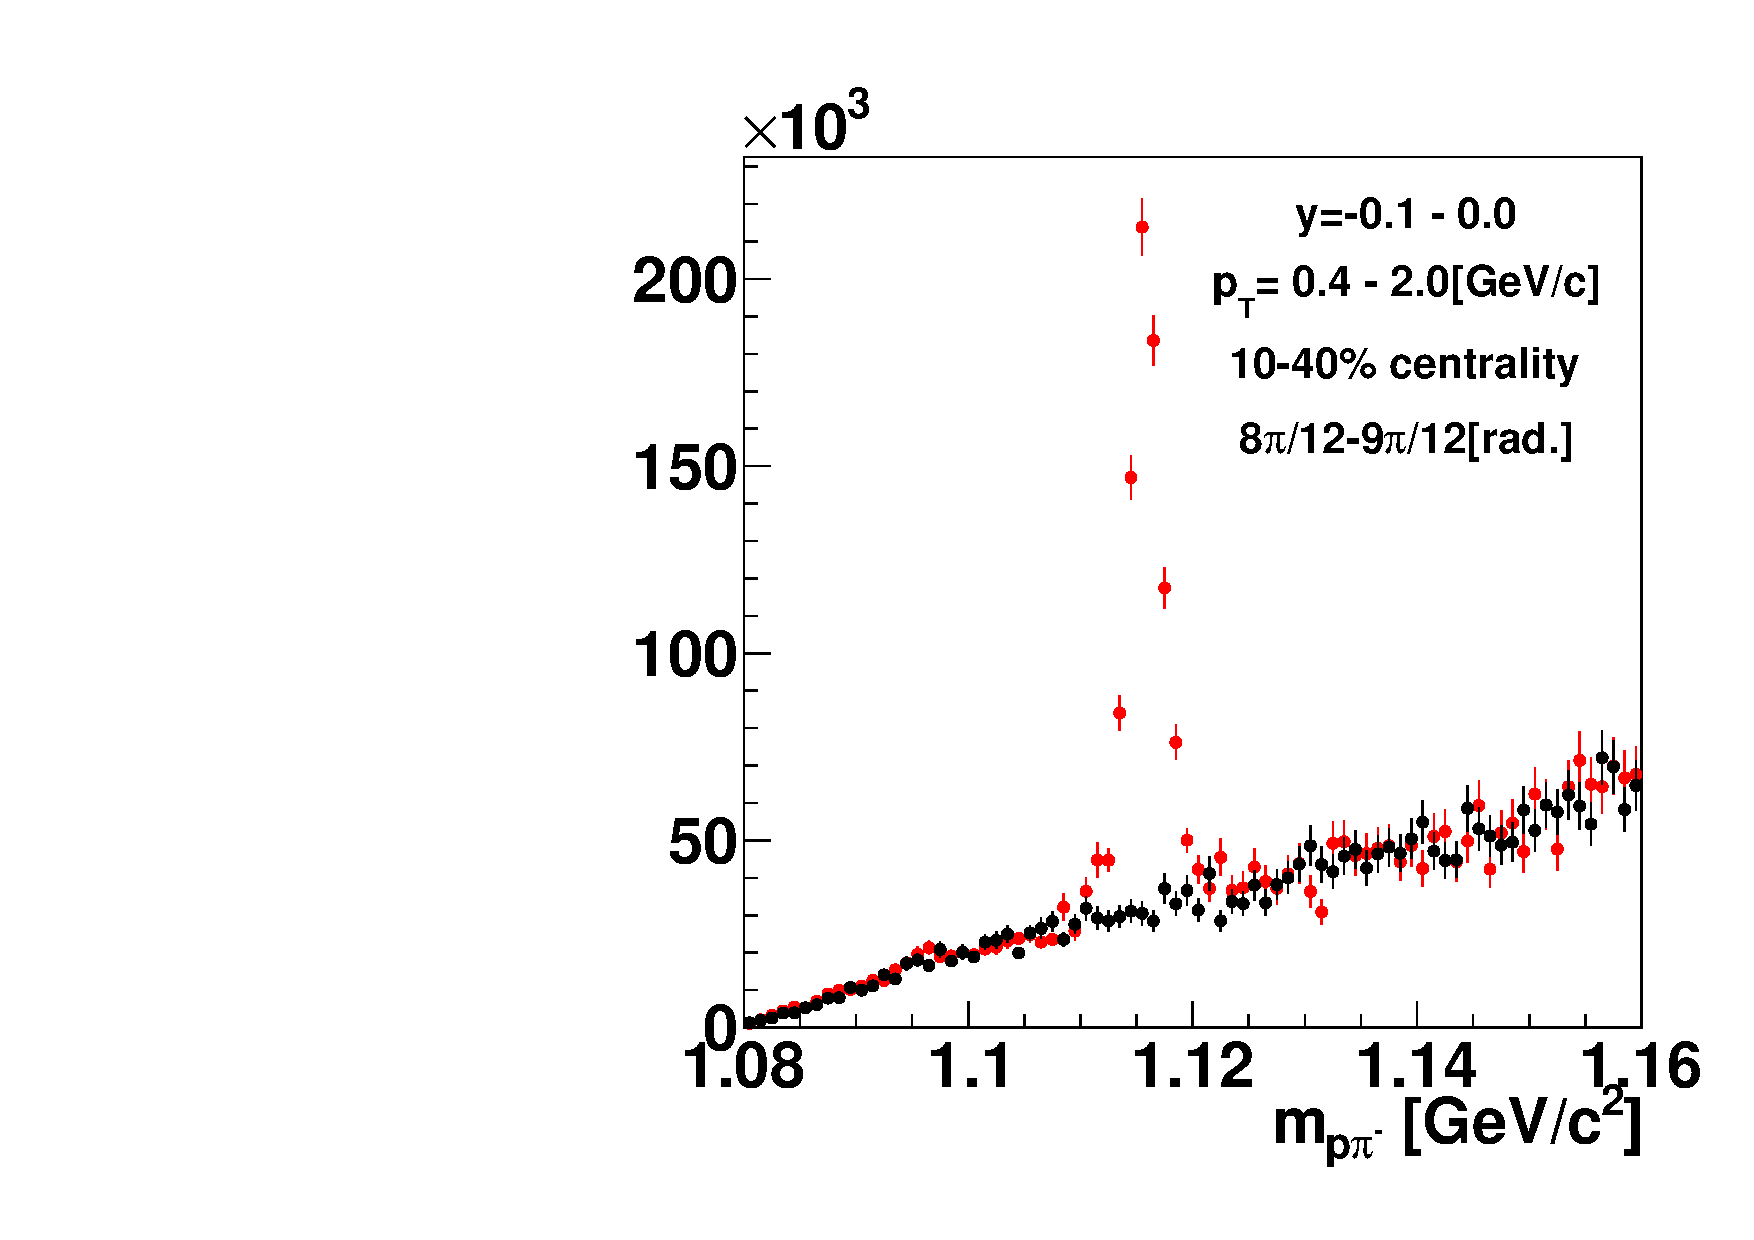
\includegraphics[width=0.14\linewidth]{chapterX/fig/ld_v1_sig/kf_ptslice0_cent1_ld_flow_phi9_rap5_check.pdf}
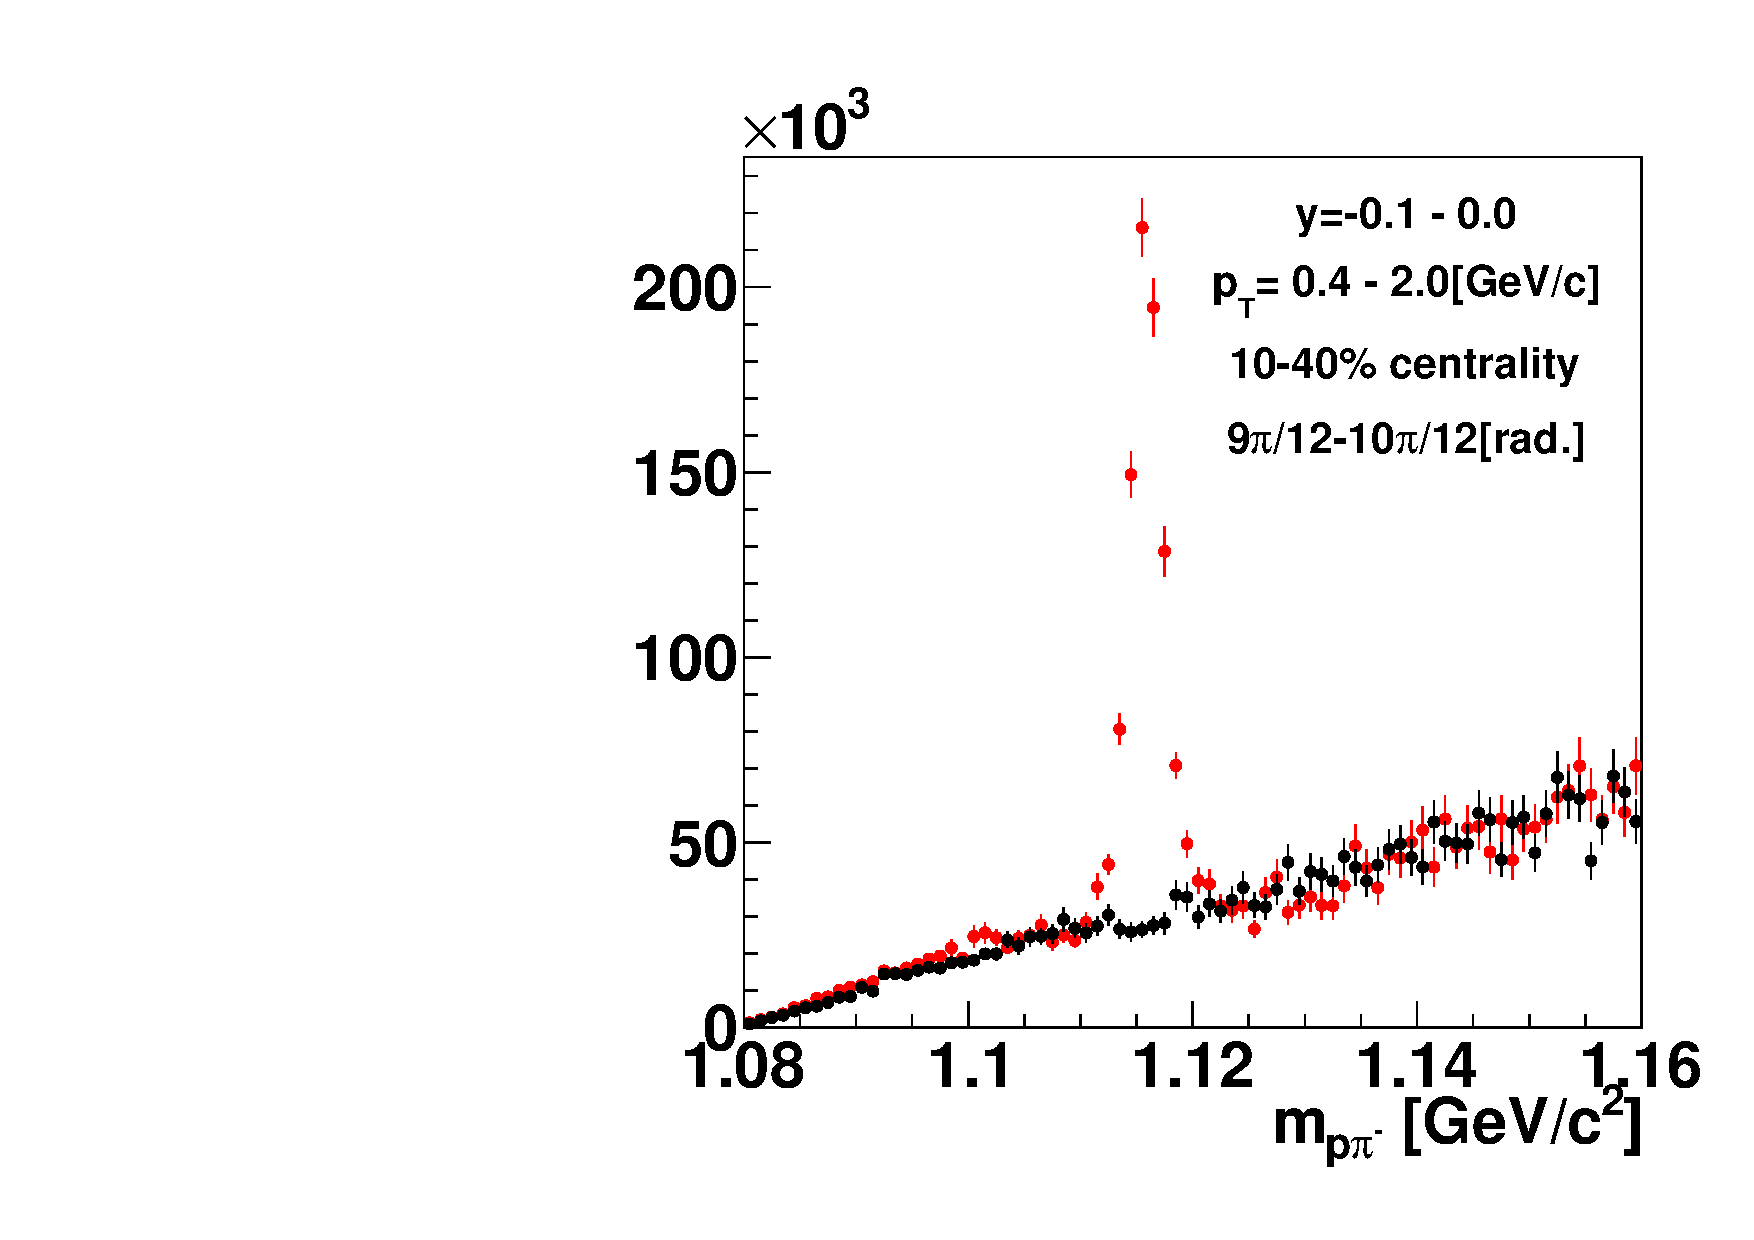
\includegraphics[width=0.14\linewidth]{chapterX/fig/ld_v1_sig/kf_ptslice0_cent1_ld_flow_phi10_rap5_check.pdf}
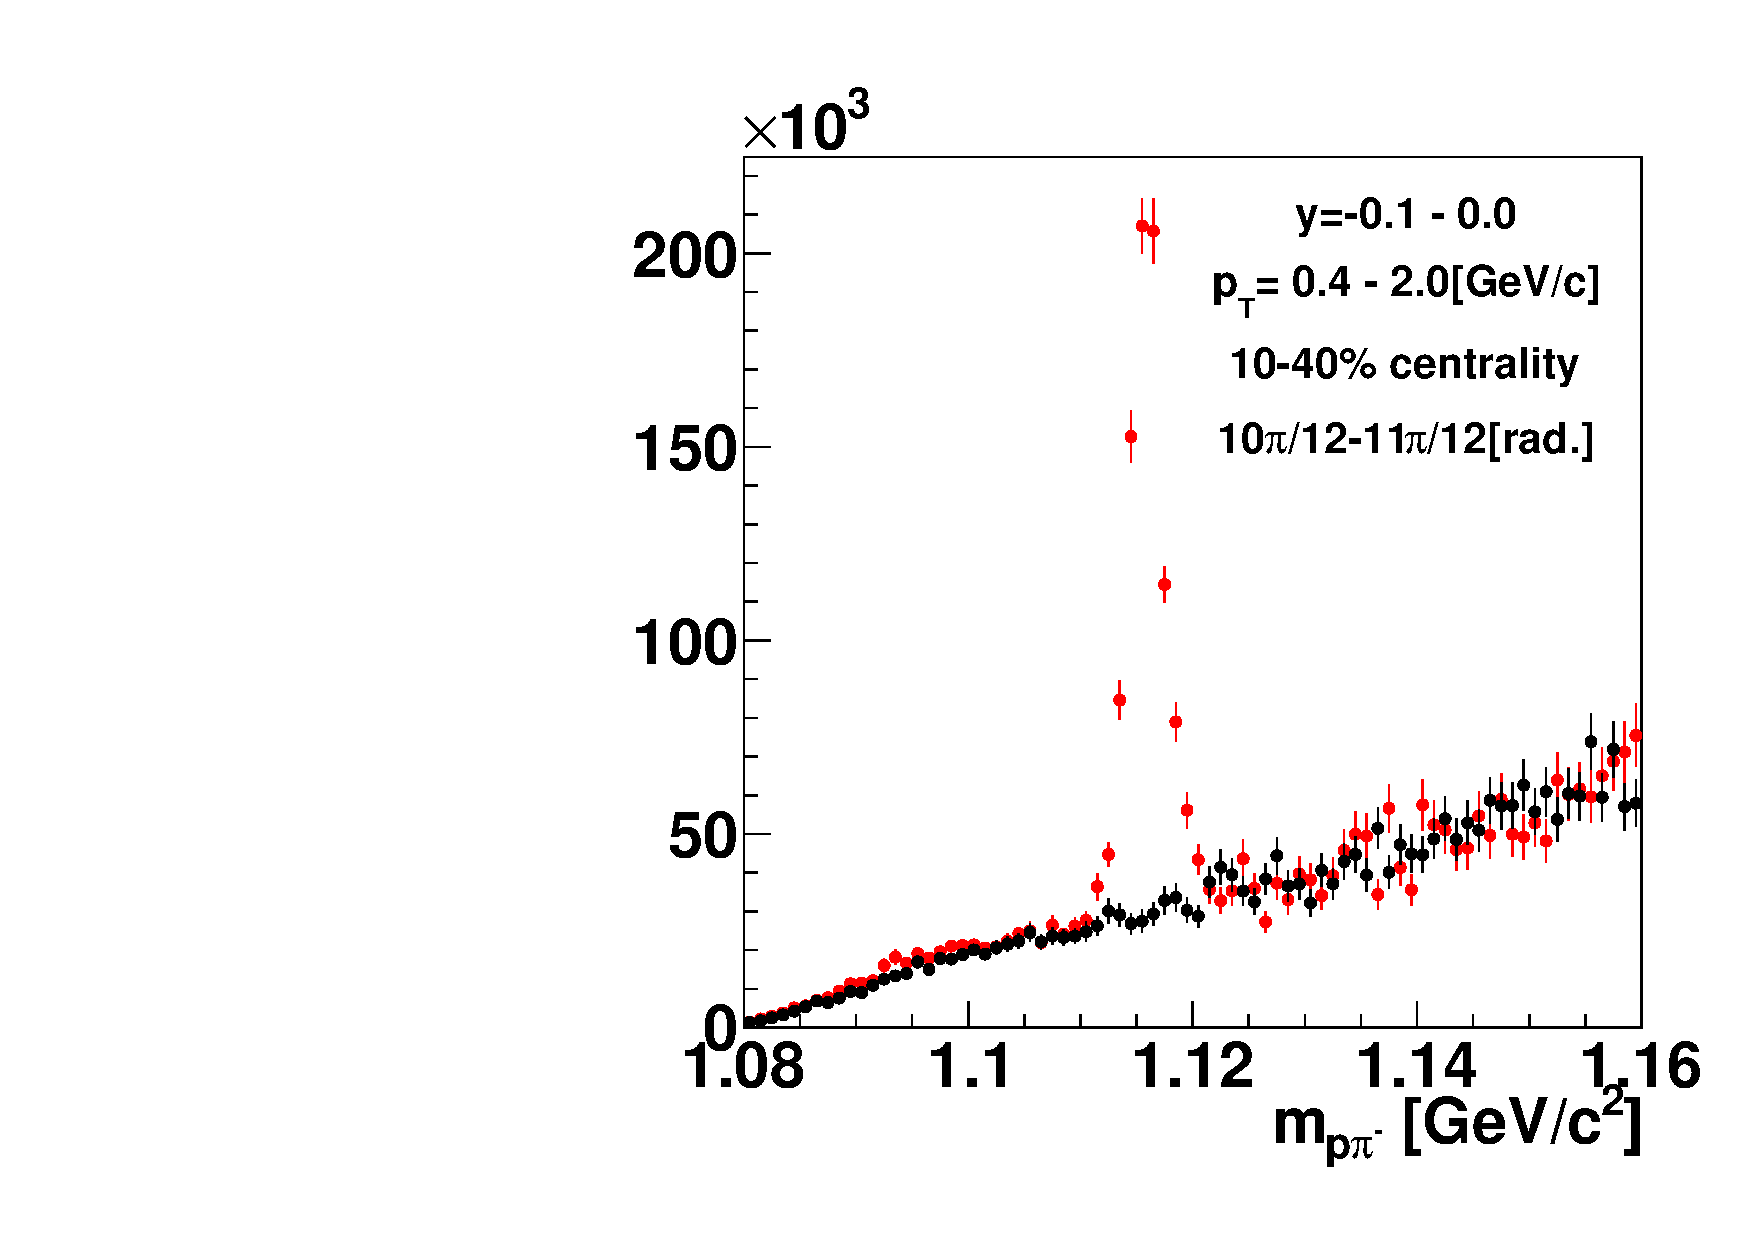
\includegraphics[width=0.14\linewidth]{chapterX/fig/ld_v1_sig/kf_ptslice0_cent1_ld_flow_phi11_rap5_check.pdf}
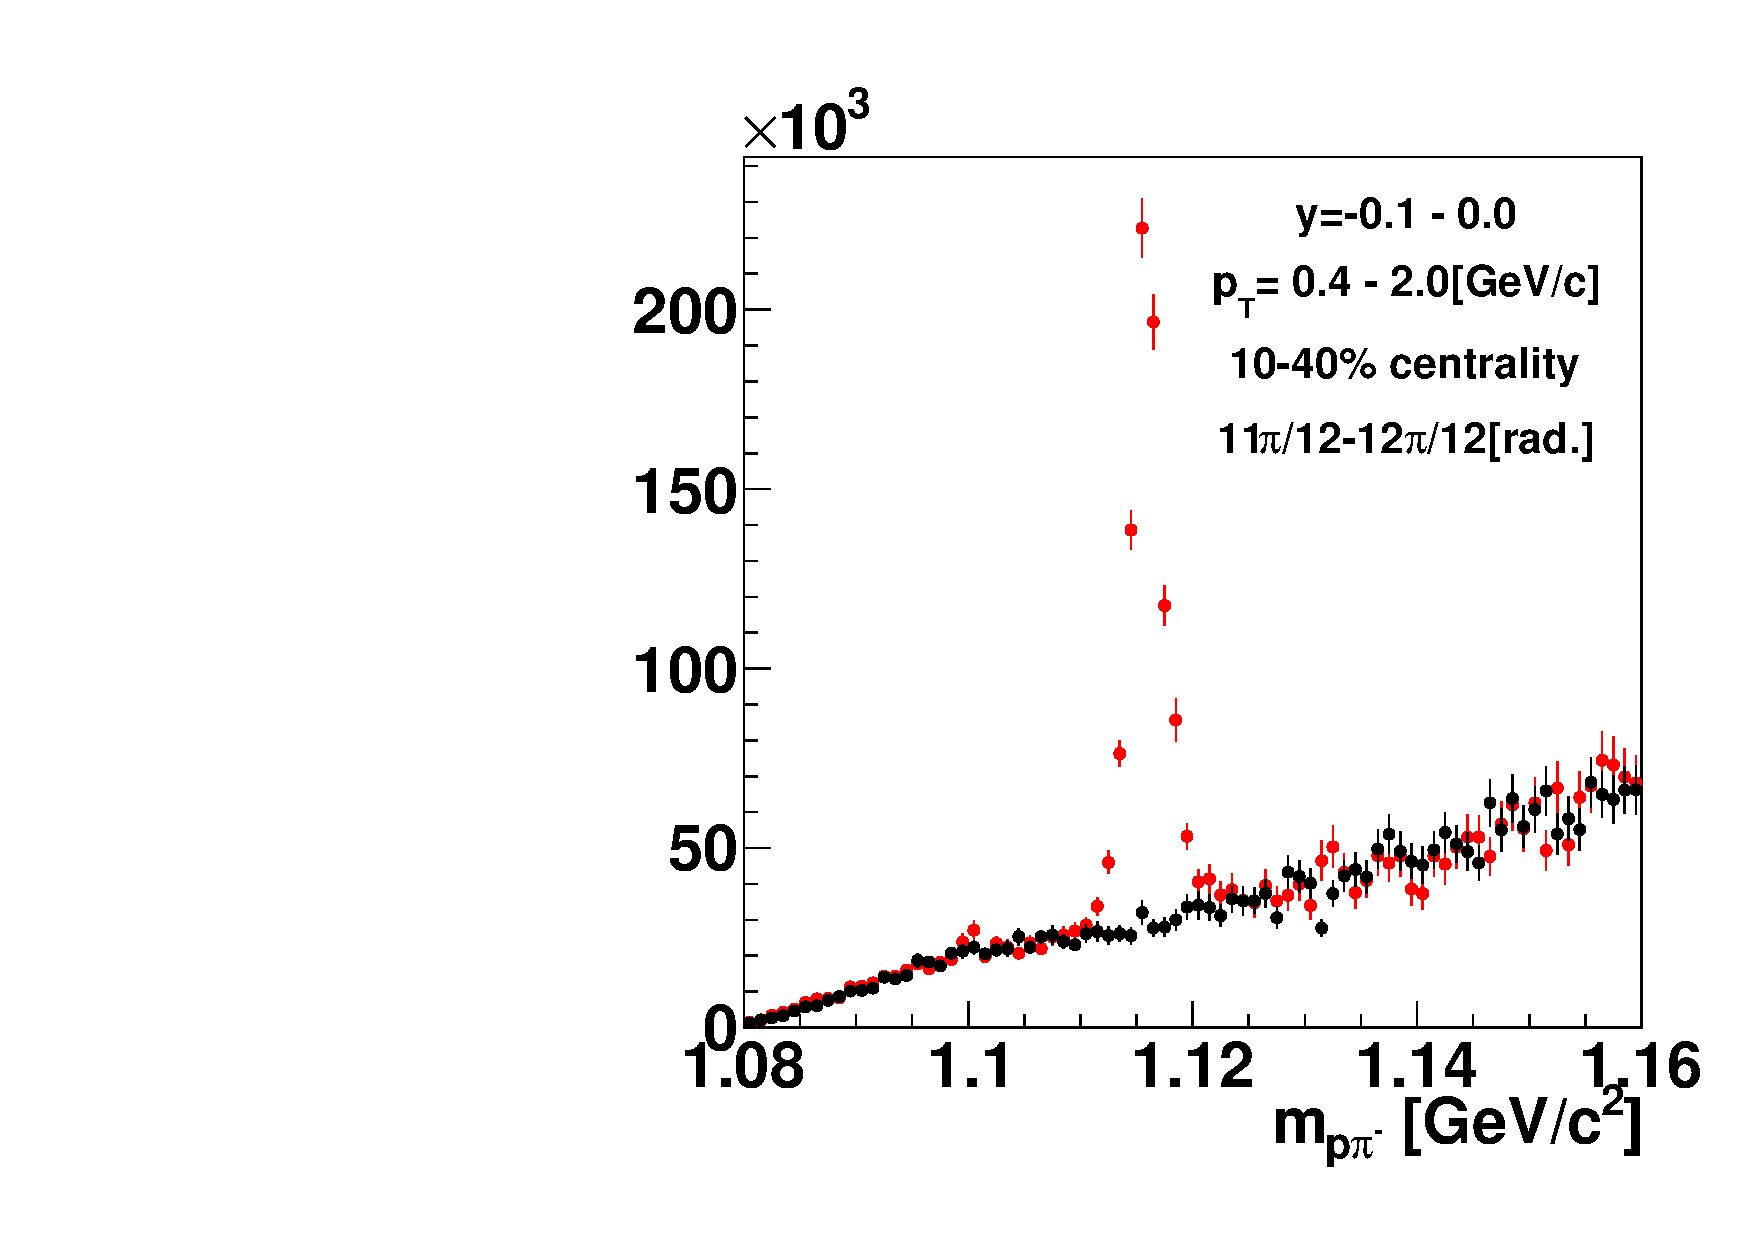
\includegraphics[width=0.14\linewidth]{chapterX/fig/ld_v1_sig/kf_ptslice0_cent1_ld_flow_phi12_rap5_check.pdf}

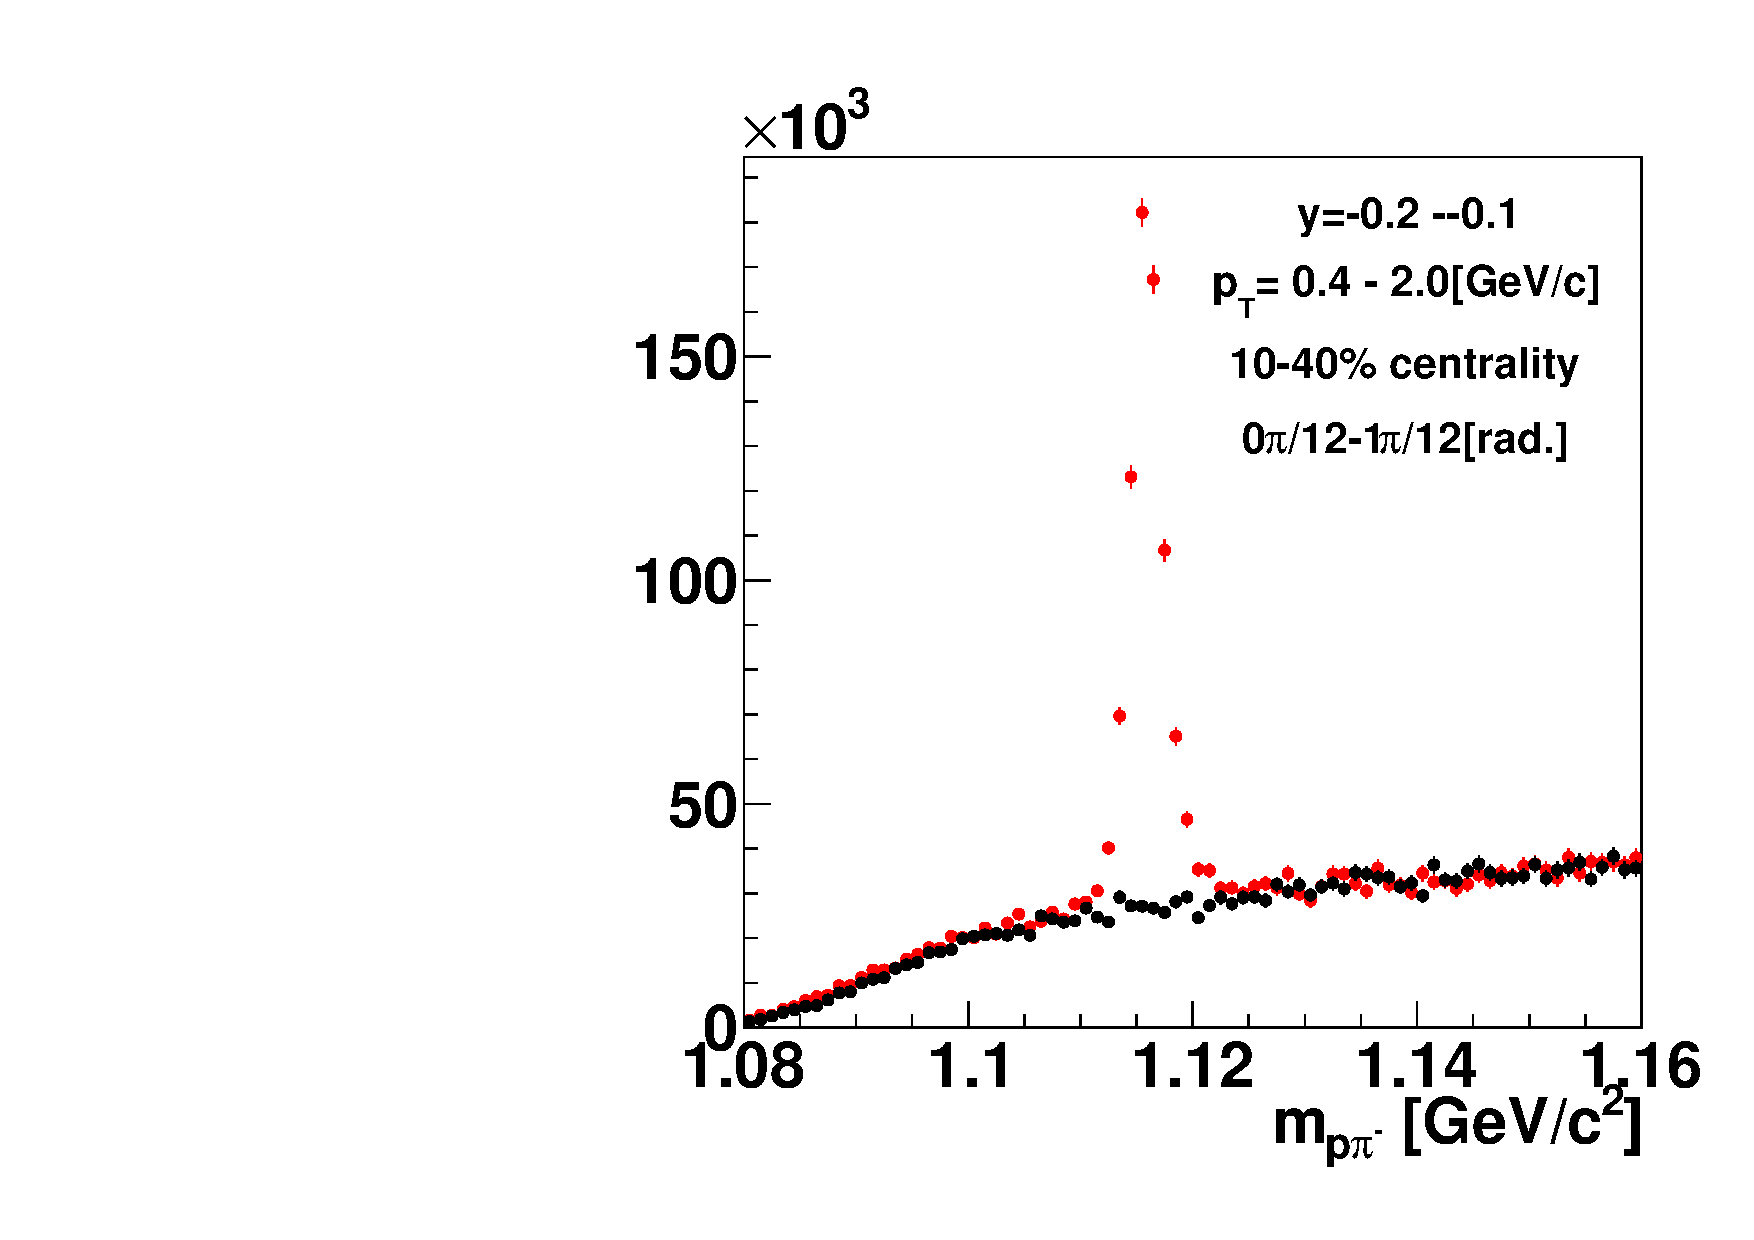
\includegraphics[width=0.14\linewidth]{chapterX/fig/ld_v1_sig/kf_ptslice0_cent1_ld_flow_phi1_rap6_check.pdf}
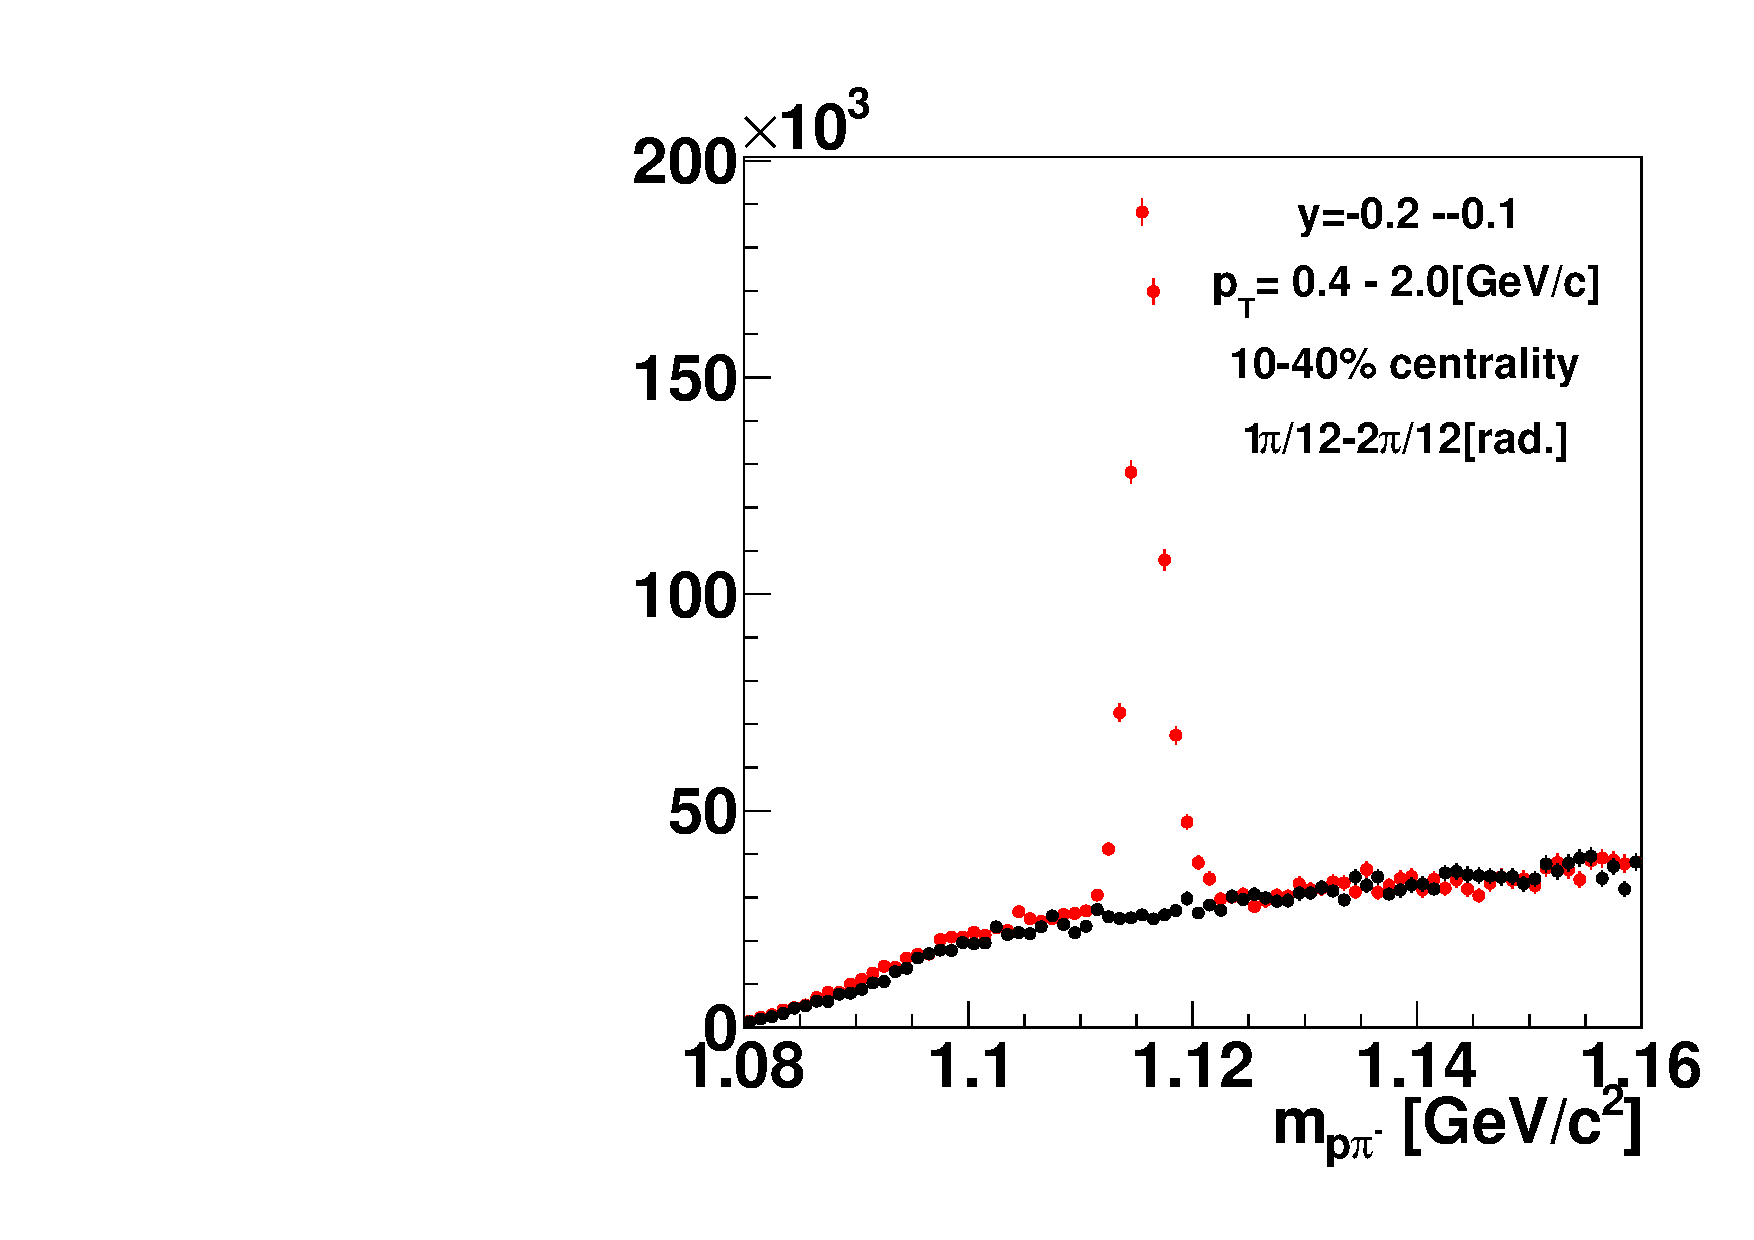
\includegraphics[width=0.14\linewidth]{chapterX/fig/ld_v1_sig/kf_ptslice0_cent1_ld_flow_phi2_rap6_check.pdf}
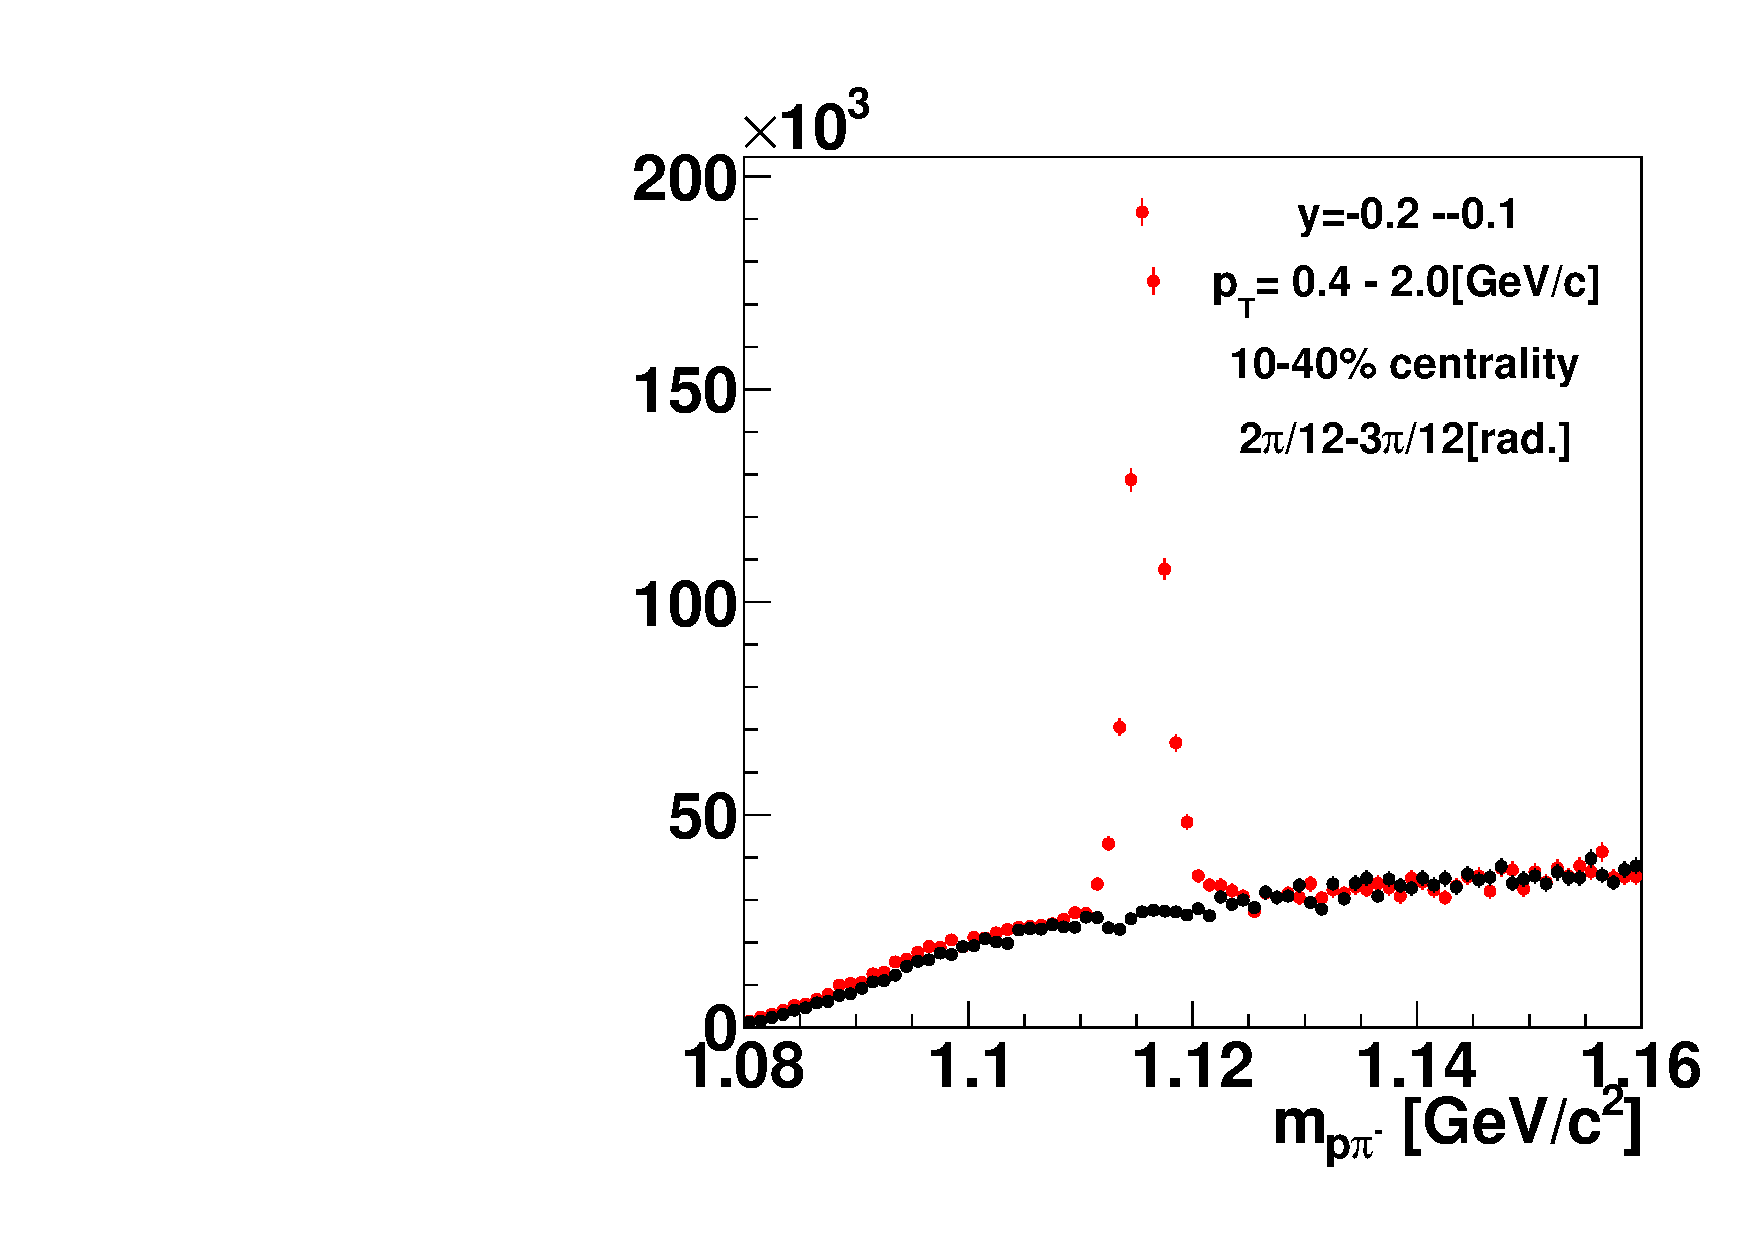
\includegraphics[width=0.14\linewidth]{chapterX/fig/ld_v1_sig/kf_ptslice0_cent1_ld_flow_phi3_rap6_check.pdf}
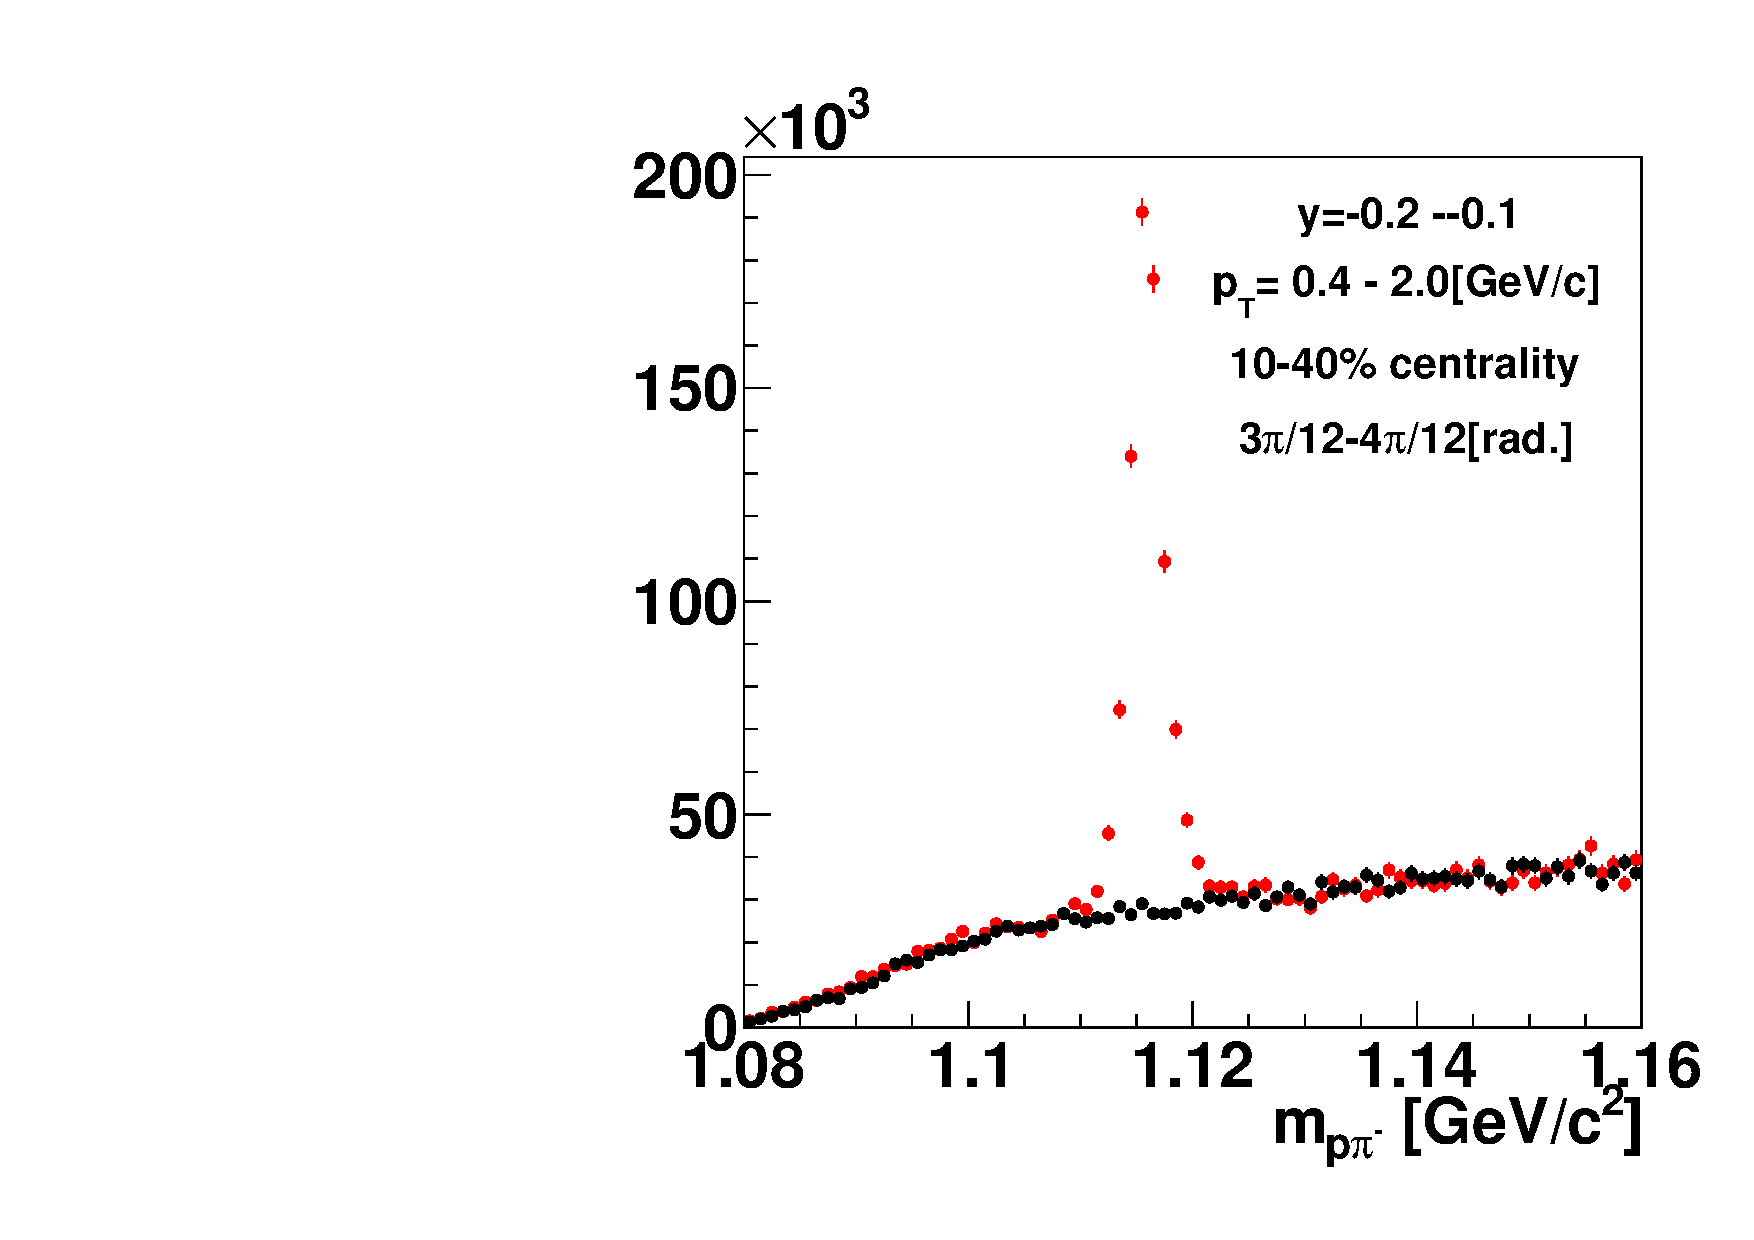
\includegraphics[width=0.14\linewidth]{chapterX/fig/ld_v1_sig/kf_ptslice0_cent1_ld_flow_phi4_rap6_check.pdf}
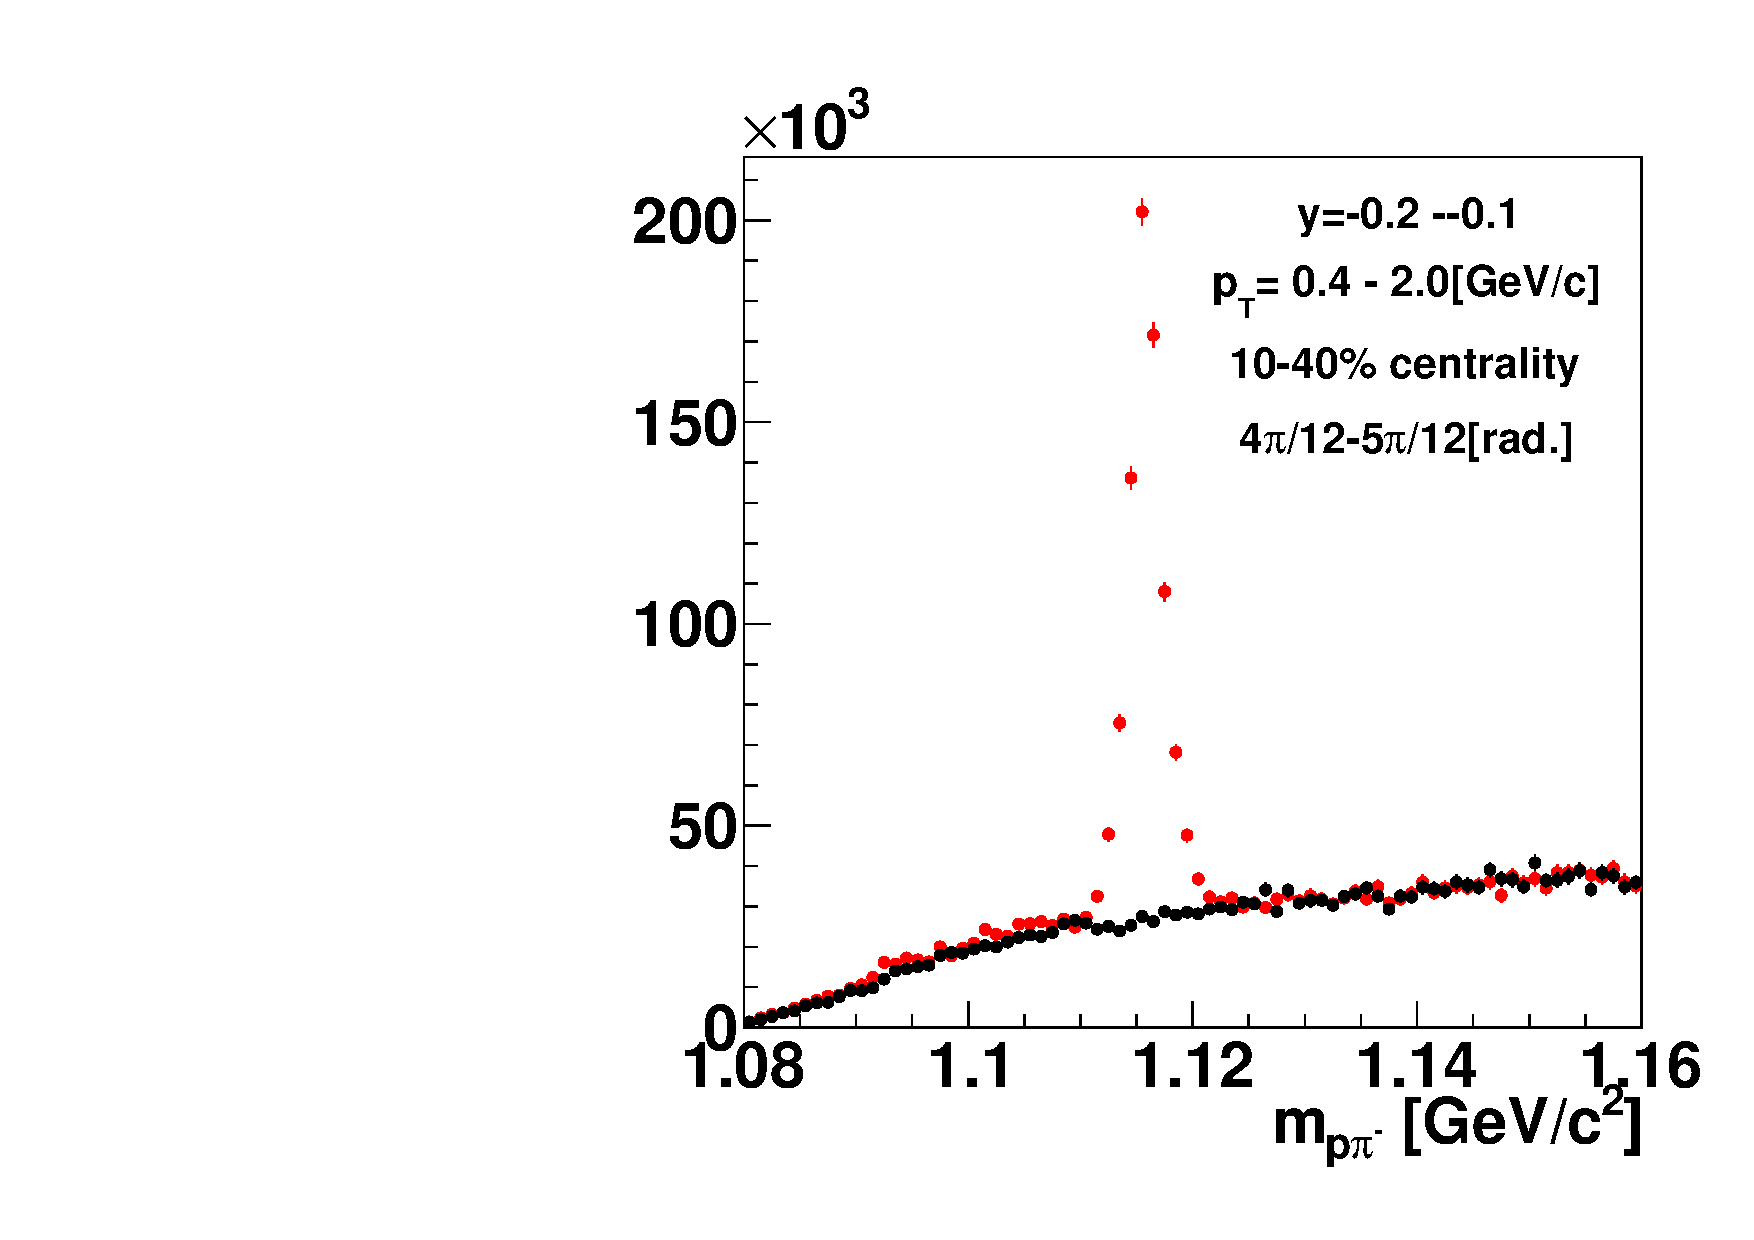
\includegraphics[width=0.14\linewidth]{chapterX/fig/ld_v1_sig/kf_ptslice0_cent1_ld_flow_phi5_rap6_check.pdf}
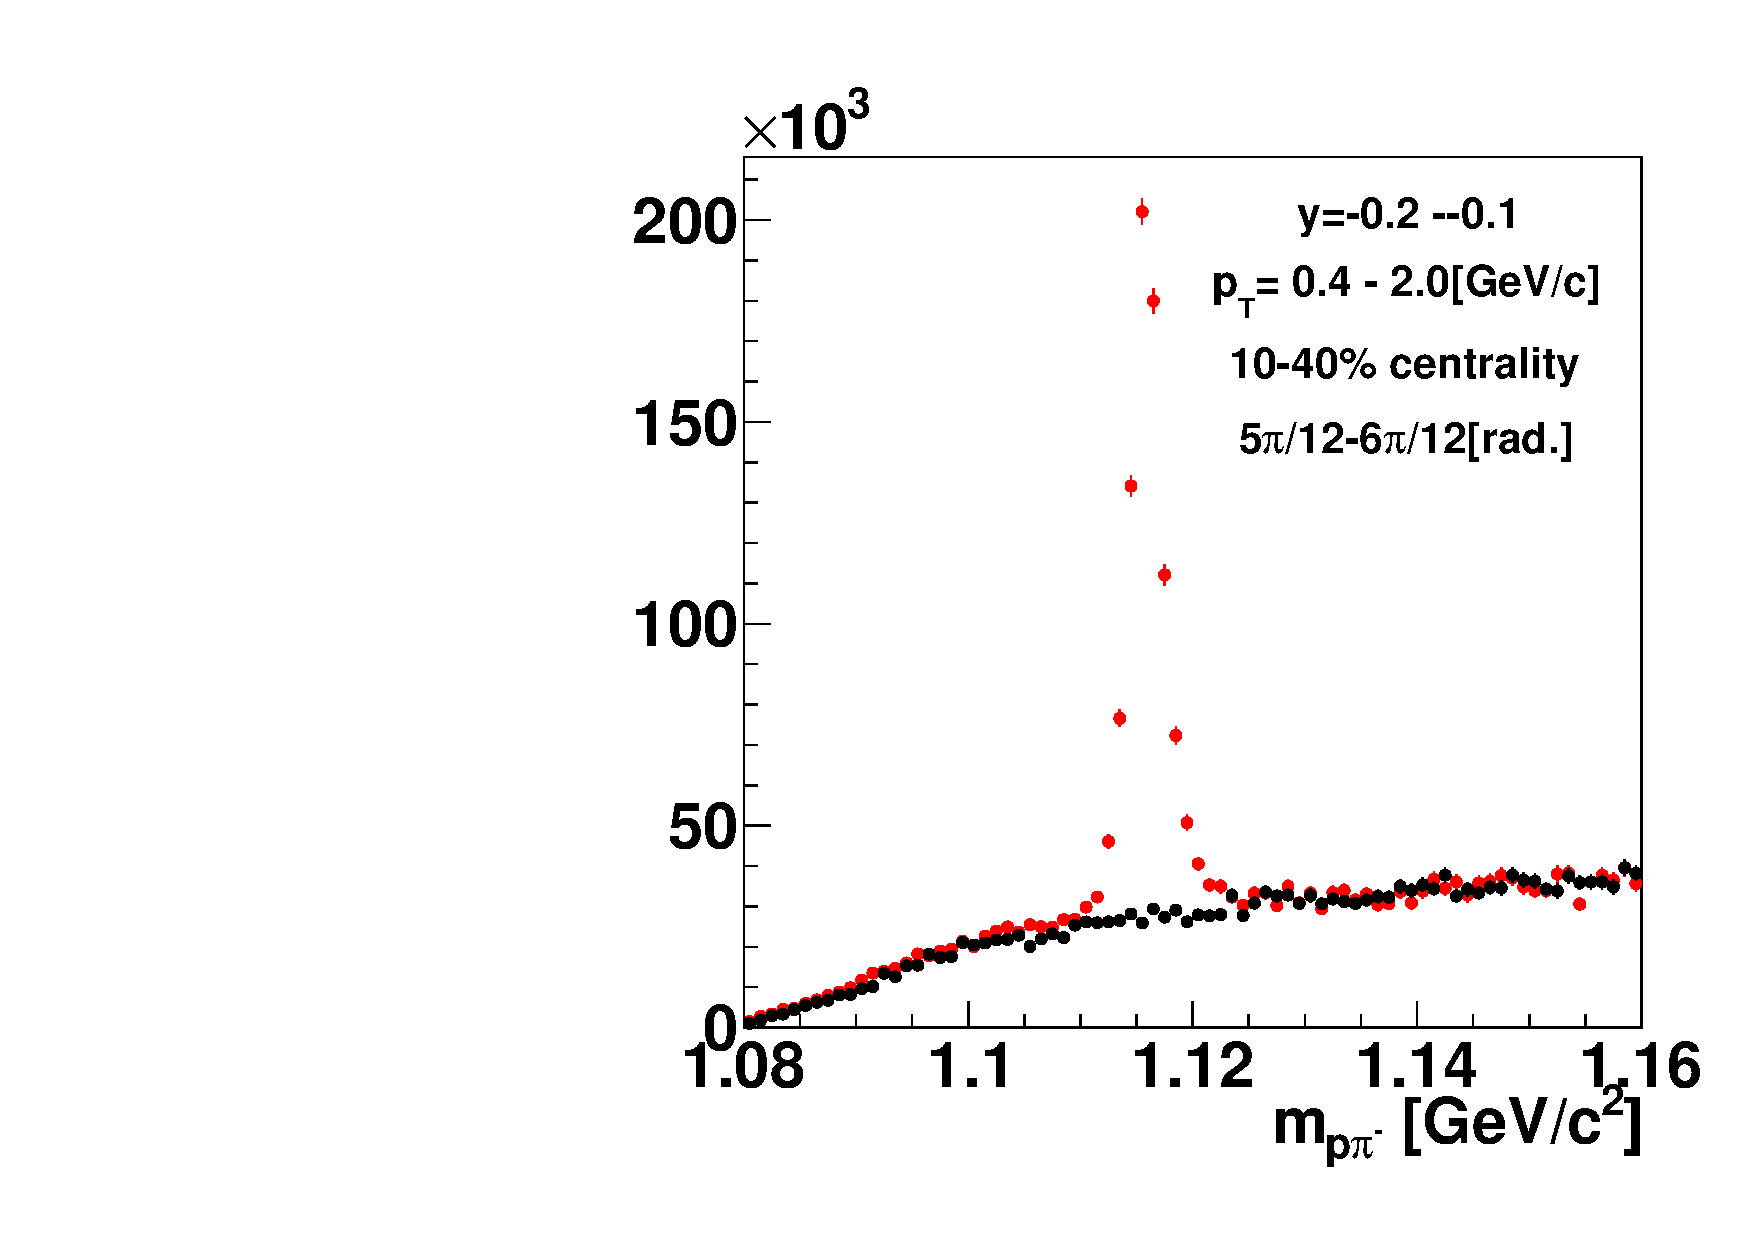
\includegraphics[width=0.14\linewidth]{chapterX/fig/ld_v1_sig/kf_ptslice0_cent1_ld_flow_phi6_rap6_check.pdf}
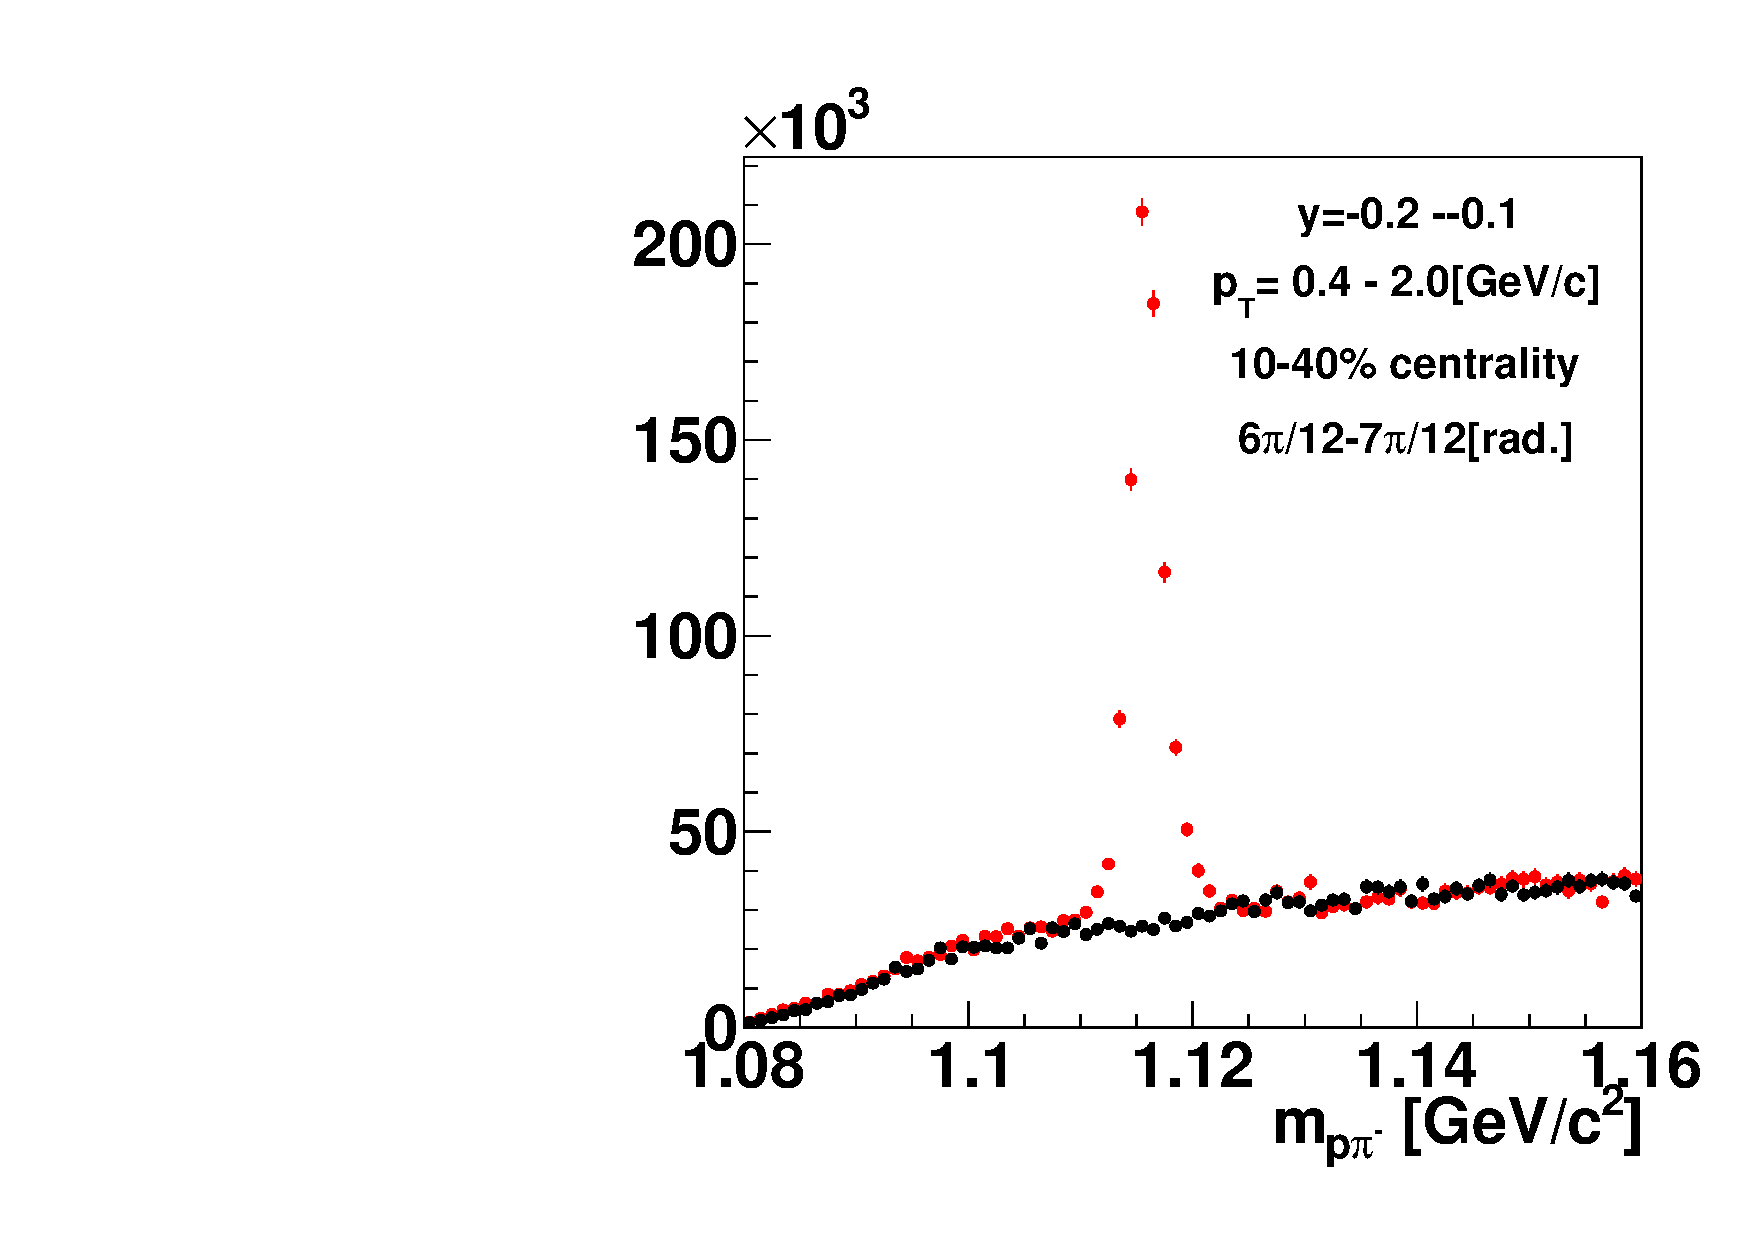
\includegraphics[width=0.14\linewidth]{chapterX/fig/ld_v1_sig/kf_ptslice0_cent1_ld_flow_phi7_rap6_check.pdf}
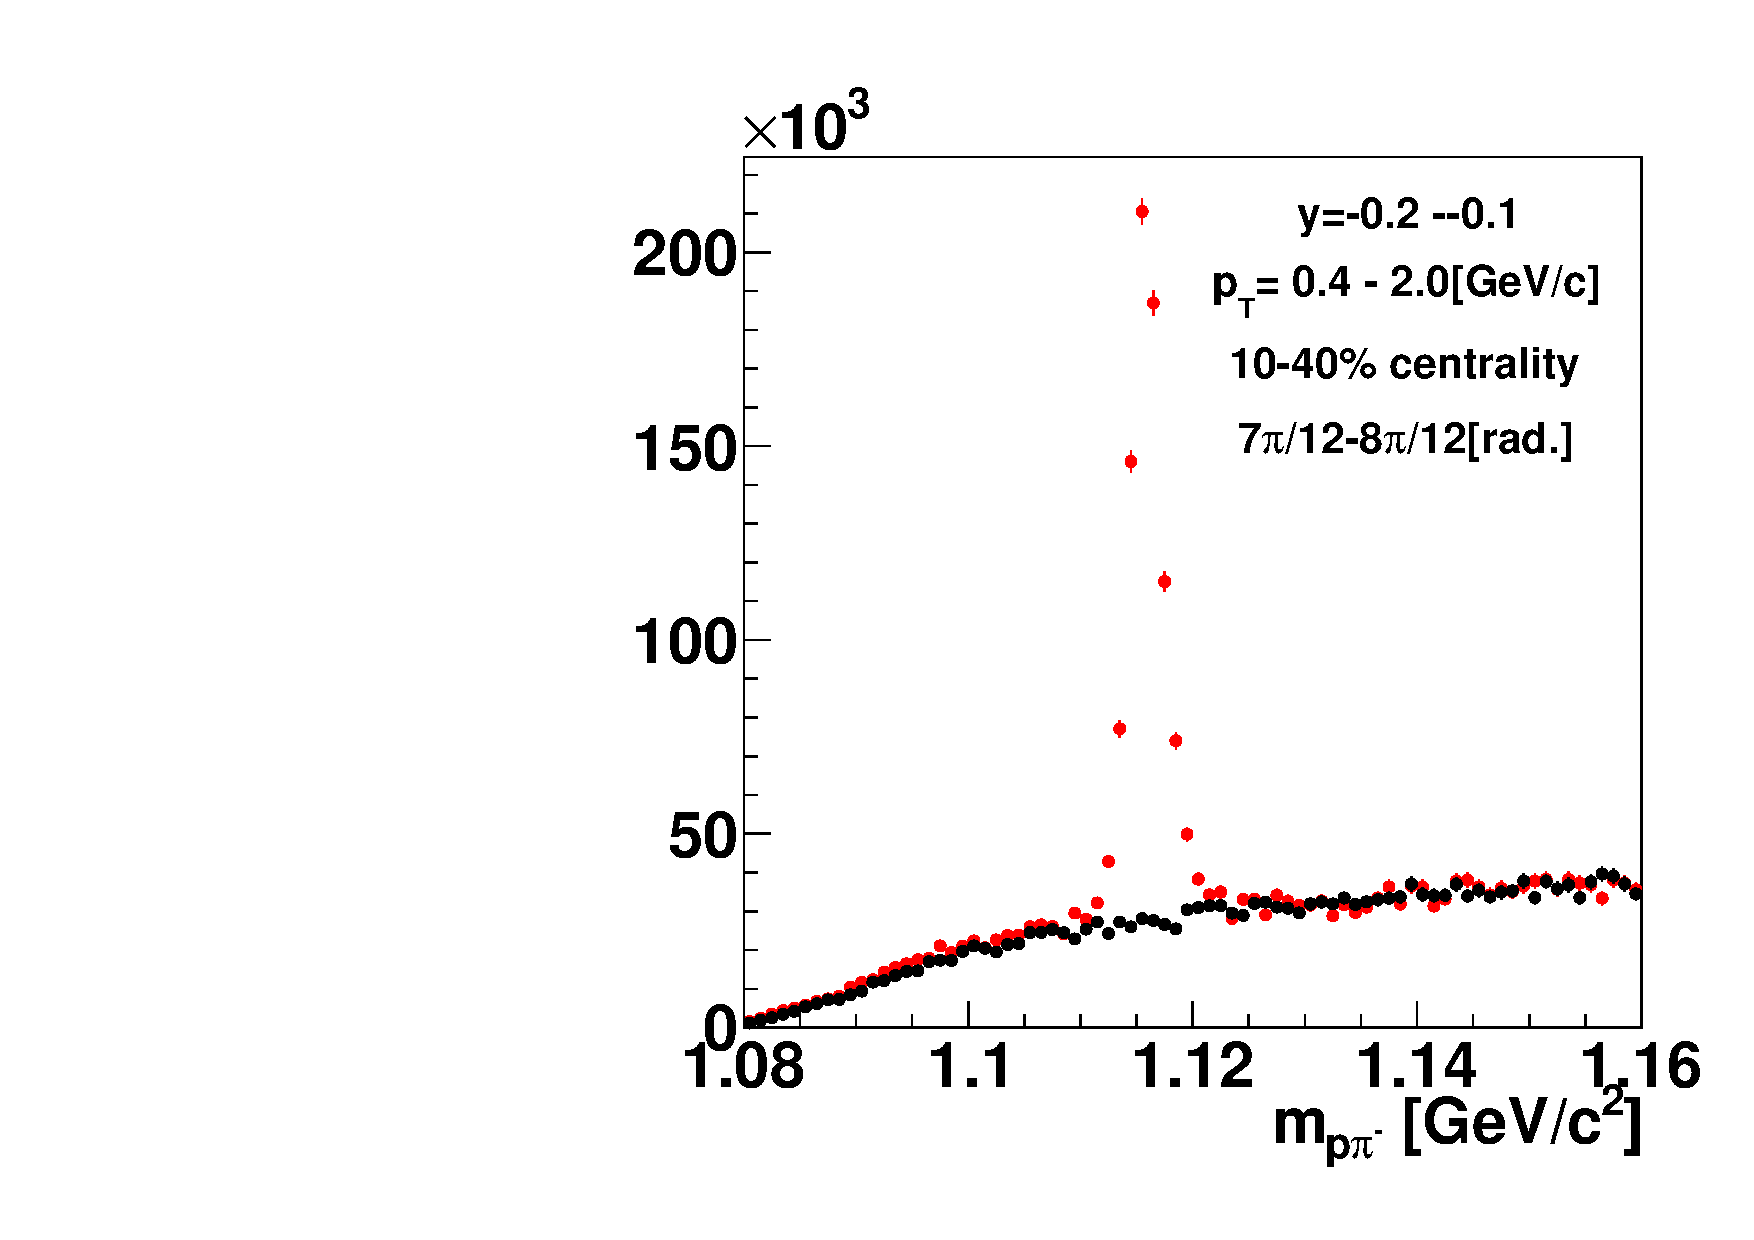
\includegraphics[width=0.14\linewidth]{chapterX/fig/ld_v1_sig/kf_ptslice0_cent1_ld_flow_phi8_rap6_check.pdf}
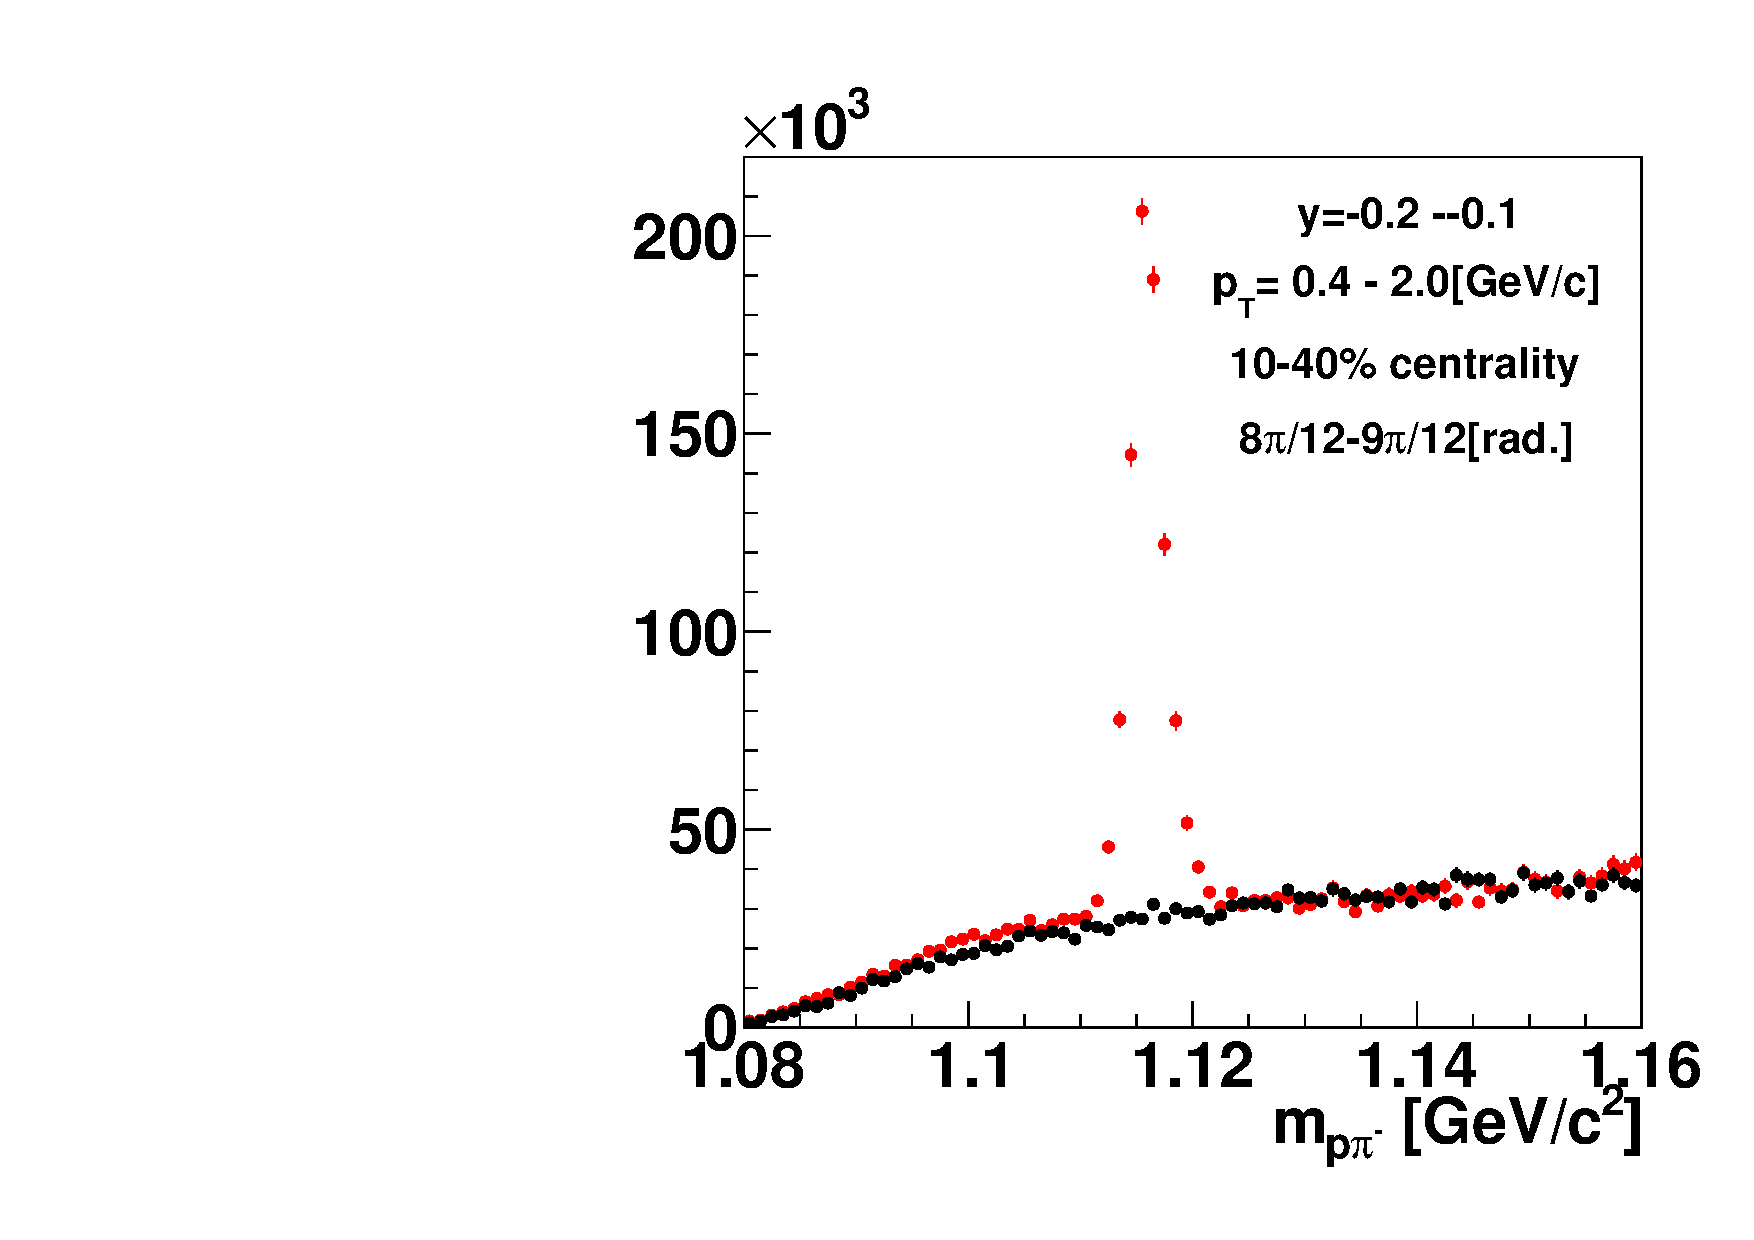
\includegraphics[width=0.14\linewidth]{chapterX/fig/ld_v1_sig/kf_ptslice0_cent1_ld_flow_phi9_rap6_check.pdf}
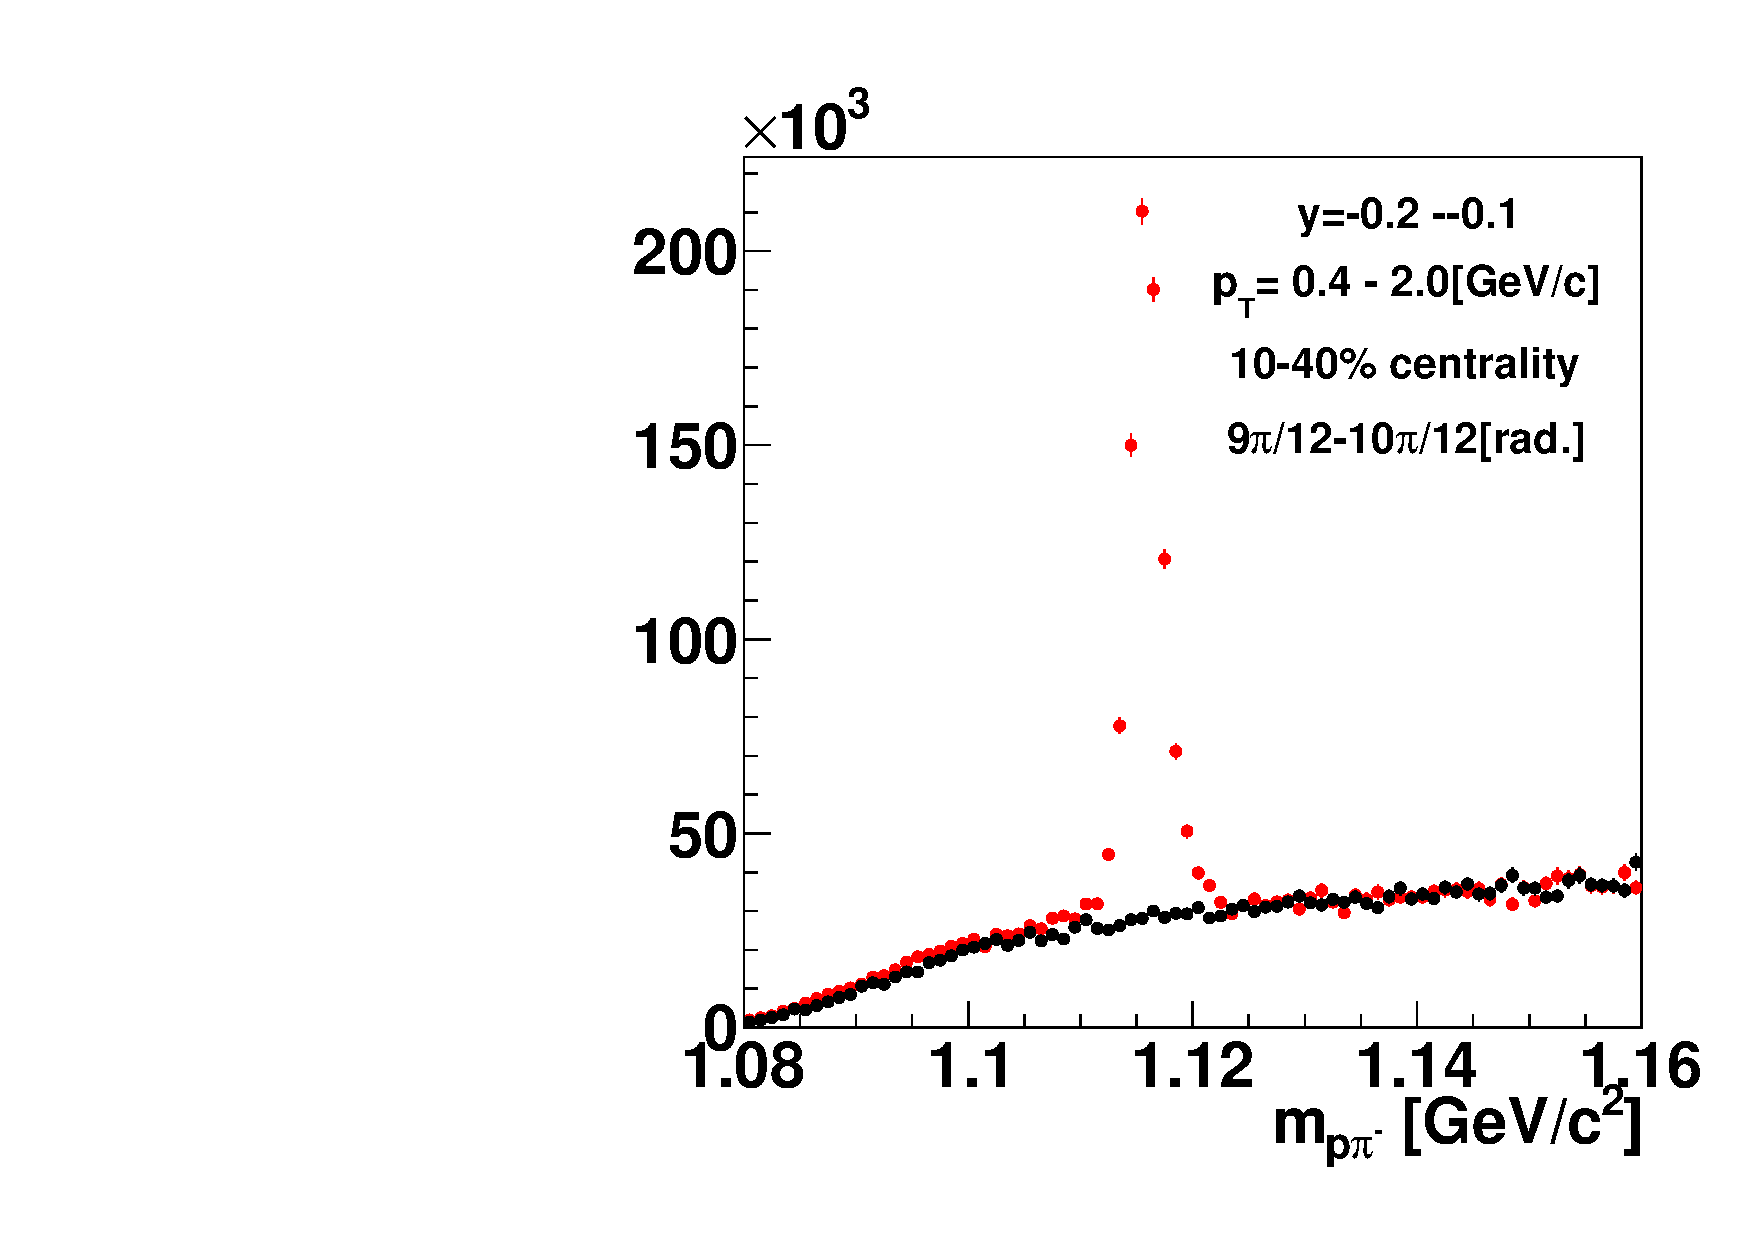
\includegraphics[width=0.14\linewidth]{chapterX/fig/ld_v1_sig/kf_ptslice0_cent1_ld_flow_phi10_rap6_check.pdf}
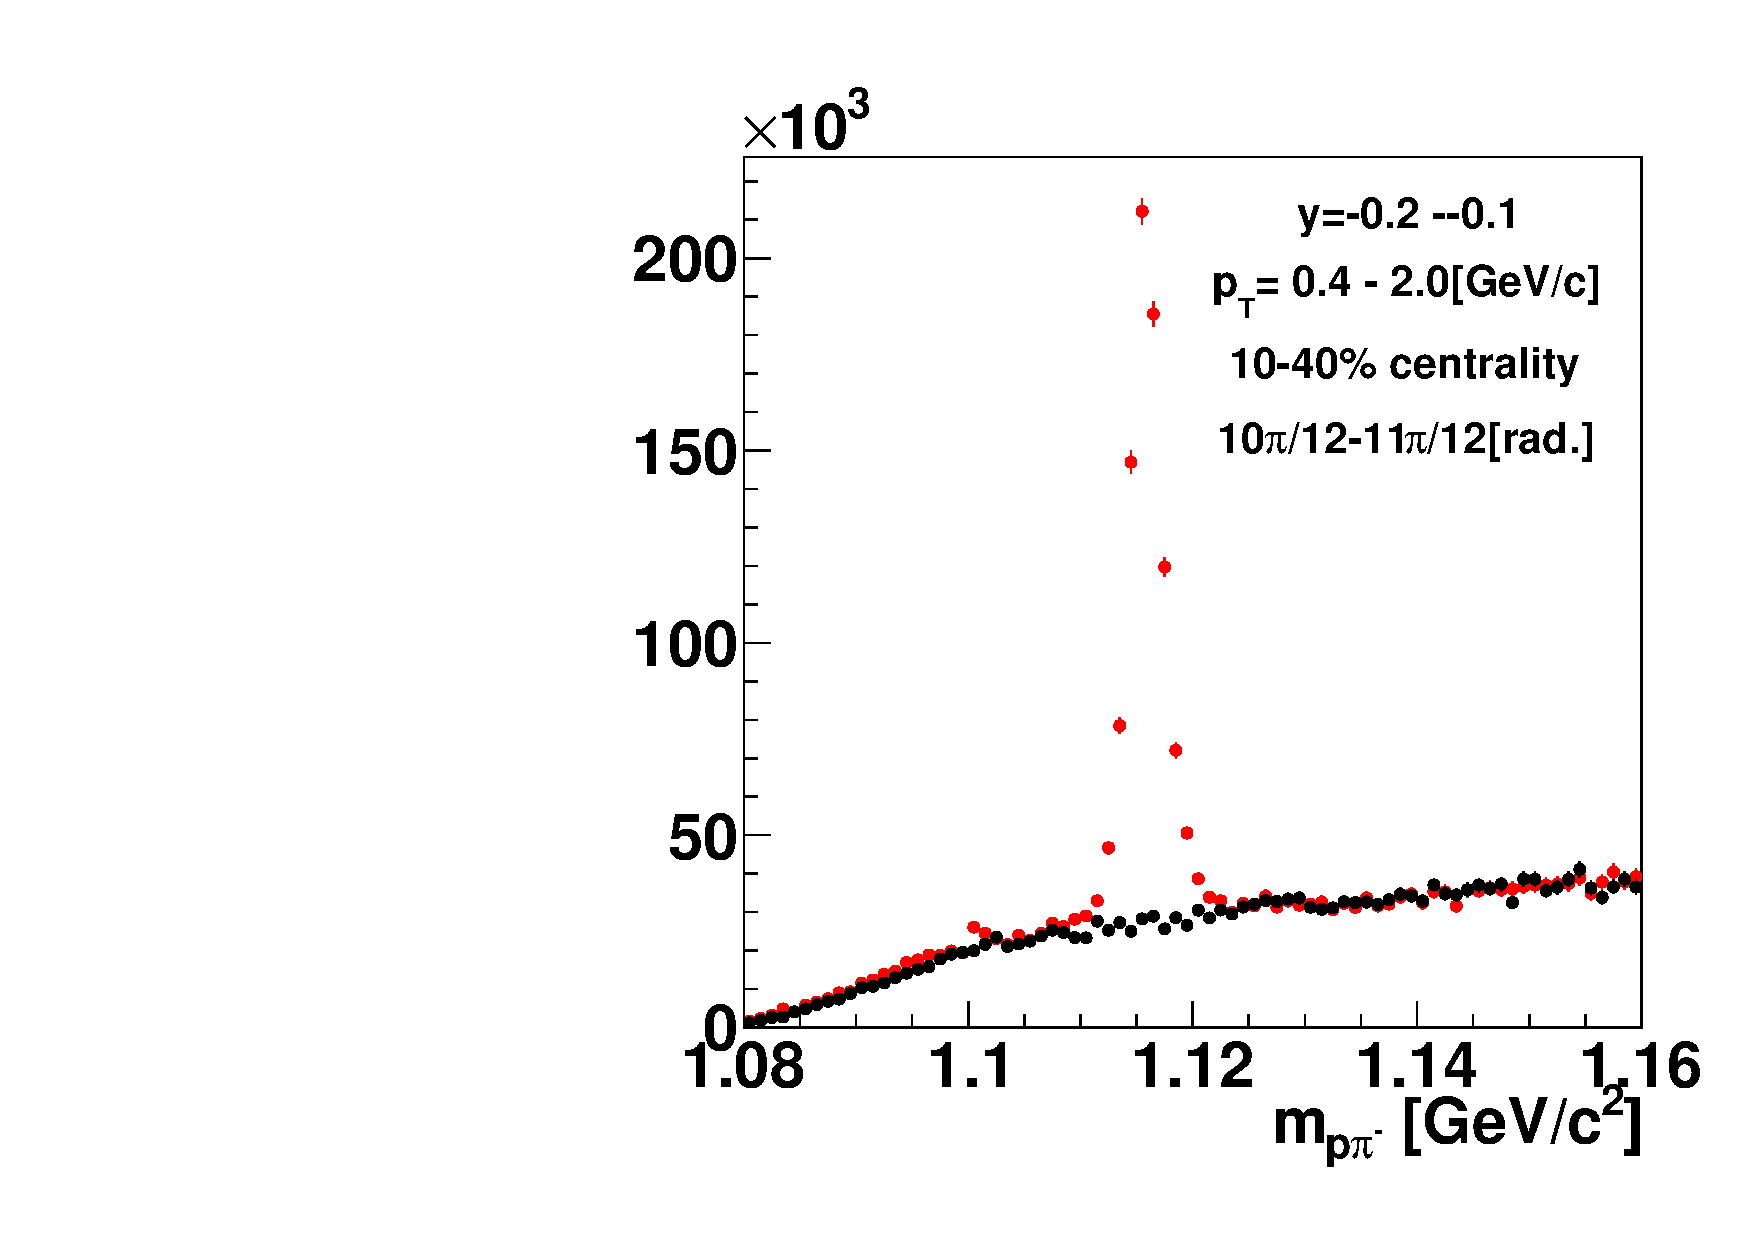
\includegraphics[width=0.14\linewidth]{chapterX/fig/ld_v1_sig/kf_ptslice0_cent1_ld_flow_phi11_rap6_check.pdf}
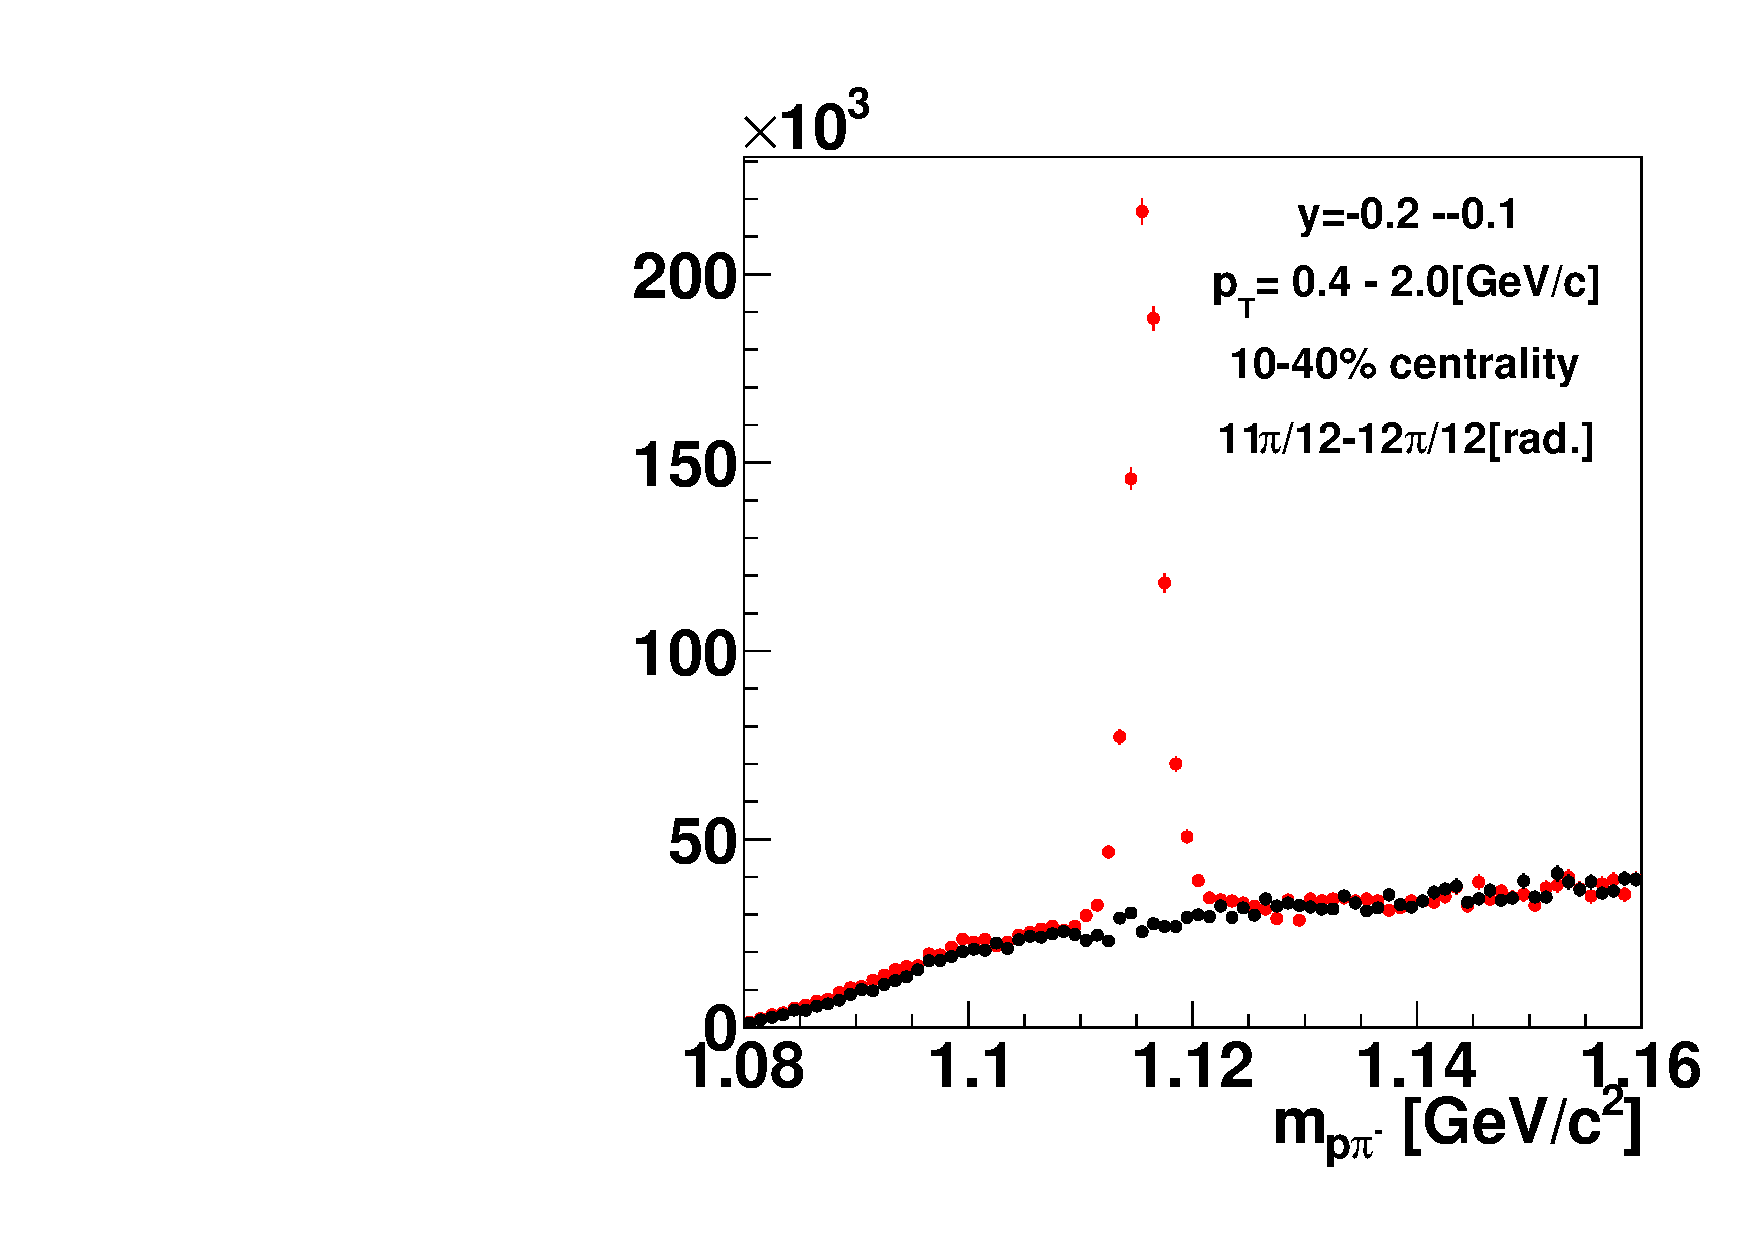
\includegraphics[width=0.14\linewidth]{chapterX/fig/ld_v1_sig/kf_ptslice0_cent1_ld_flow_phi12_rap6_check.pdf}

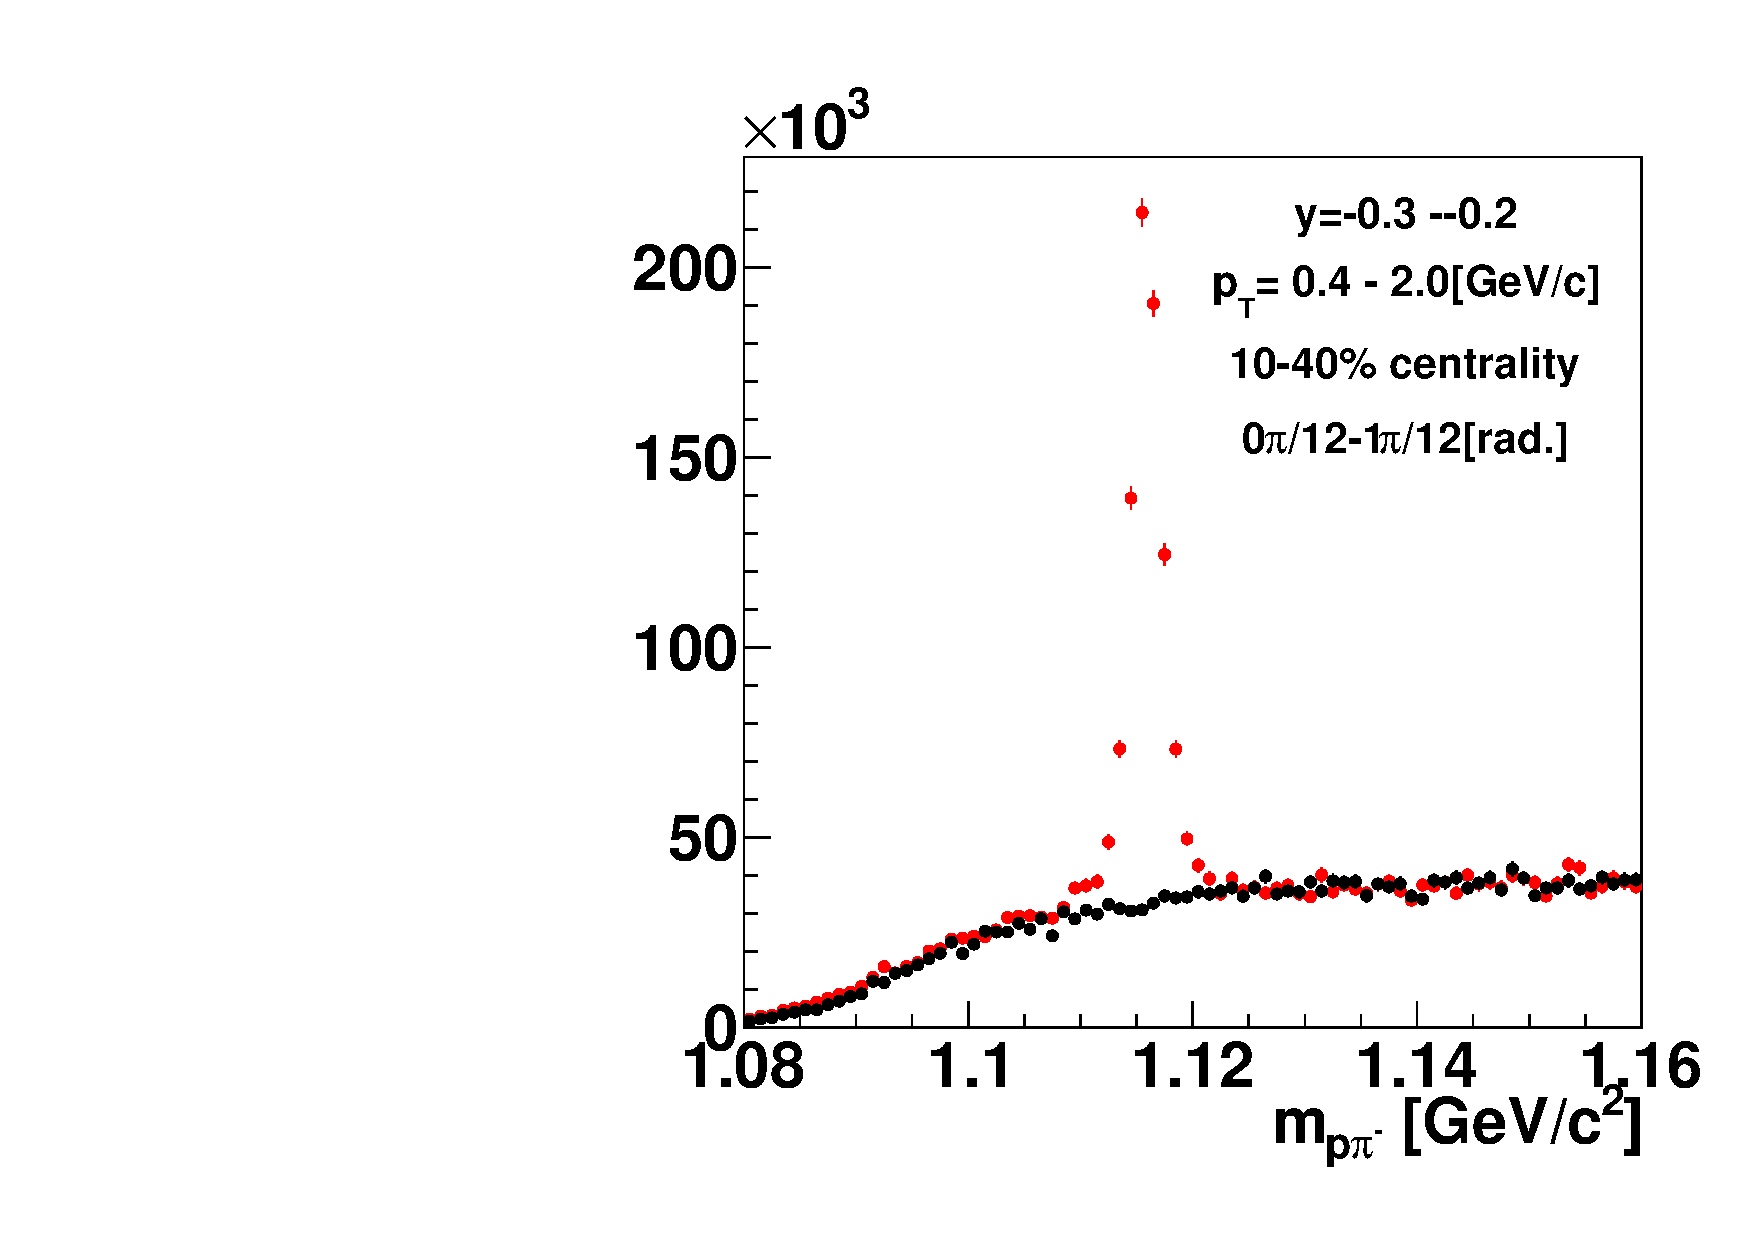
\includegraphics[width=0.14\linewidth]{chapterX/fig/ld_v1_sig/kf_ptslice0_cent1_ld_flow_phi1_rap7_check.pdf}
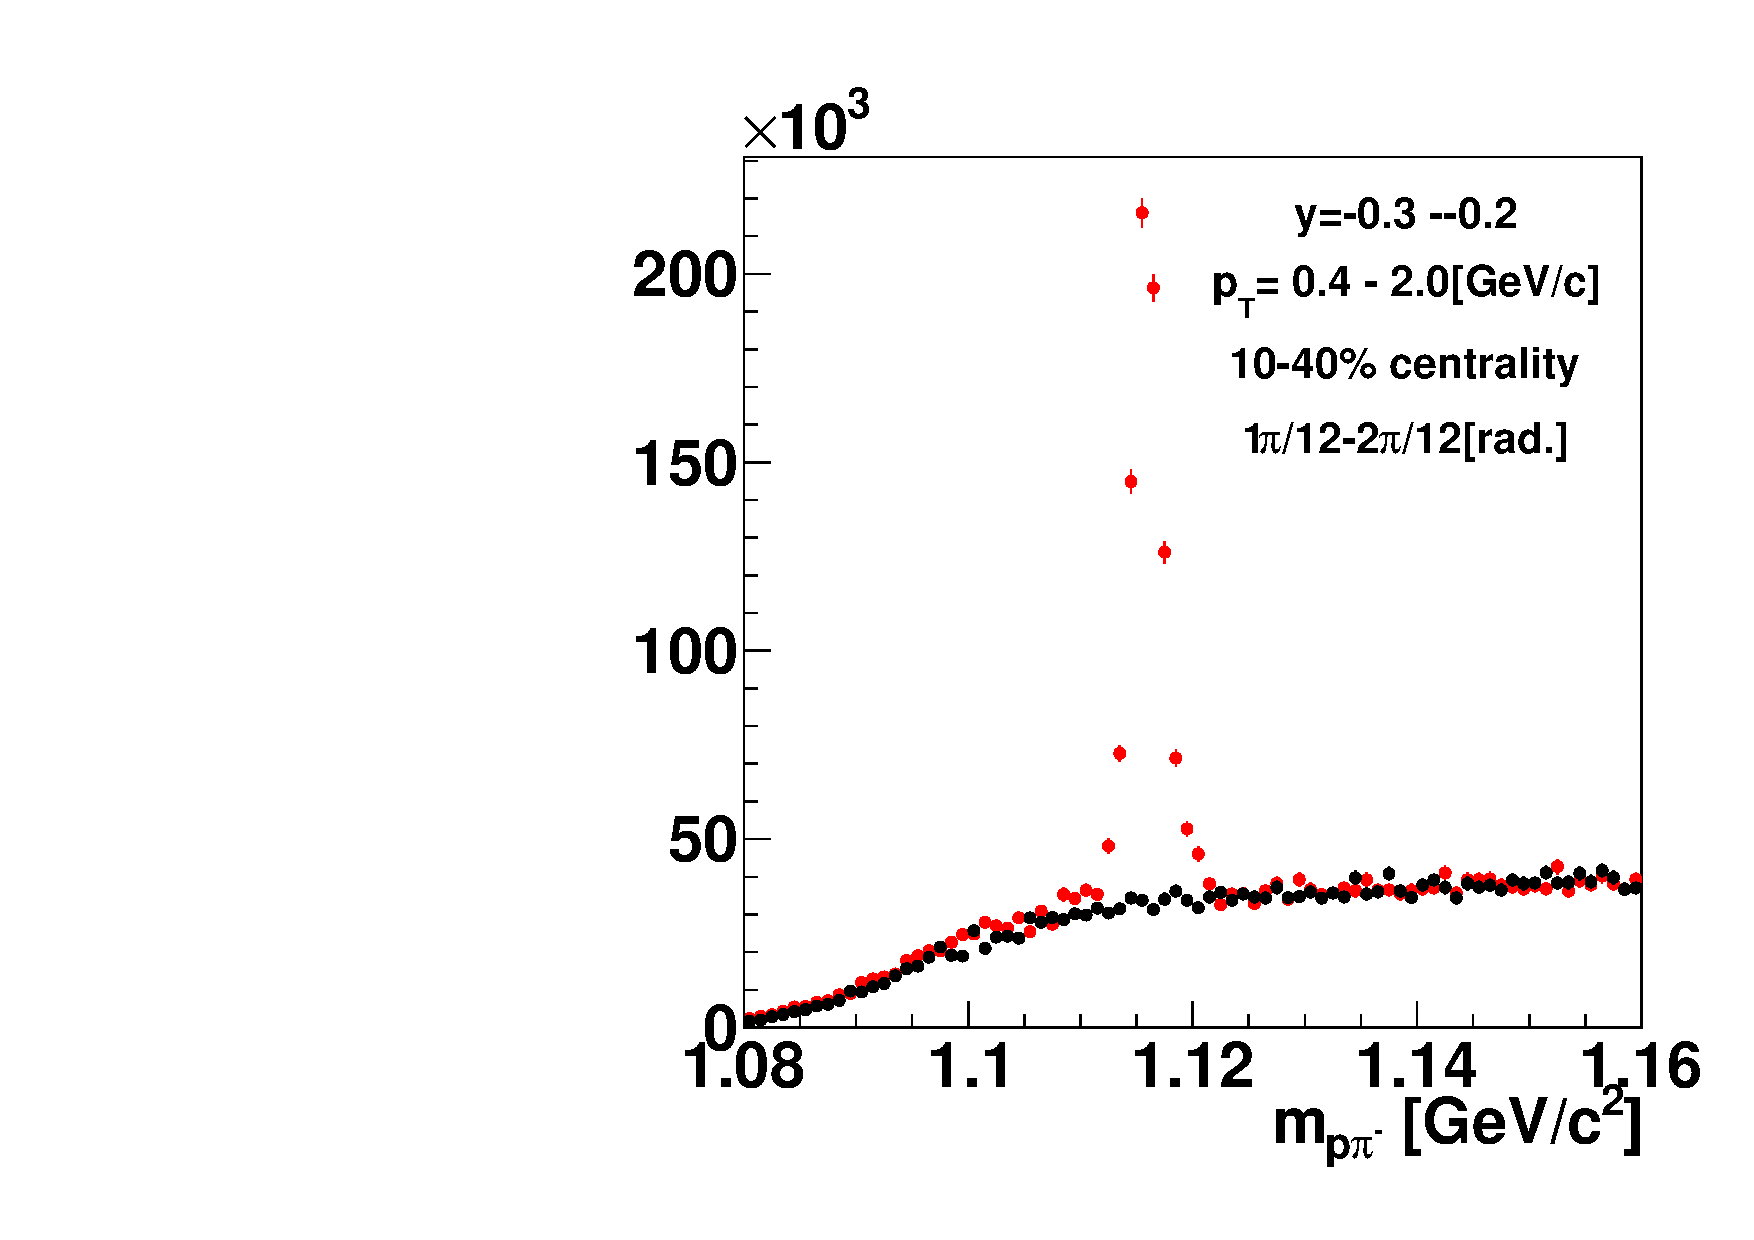
\includegraphics[width=0.14\linewidth]{chapterX/fig/ld_v1_sig/kf_ptslice0_cent1_ld_flow_phi2_rap7_check.pdf}
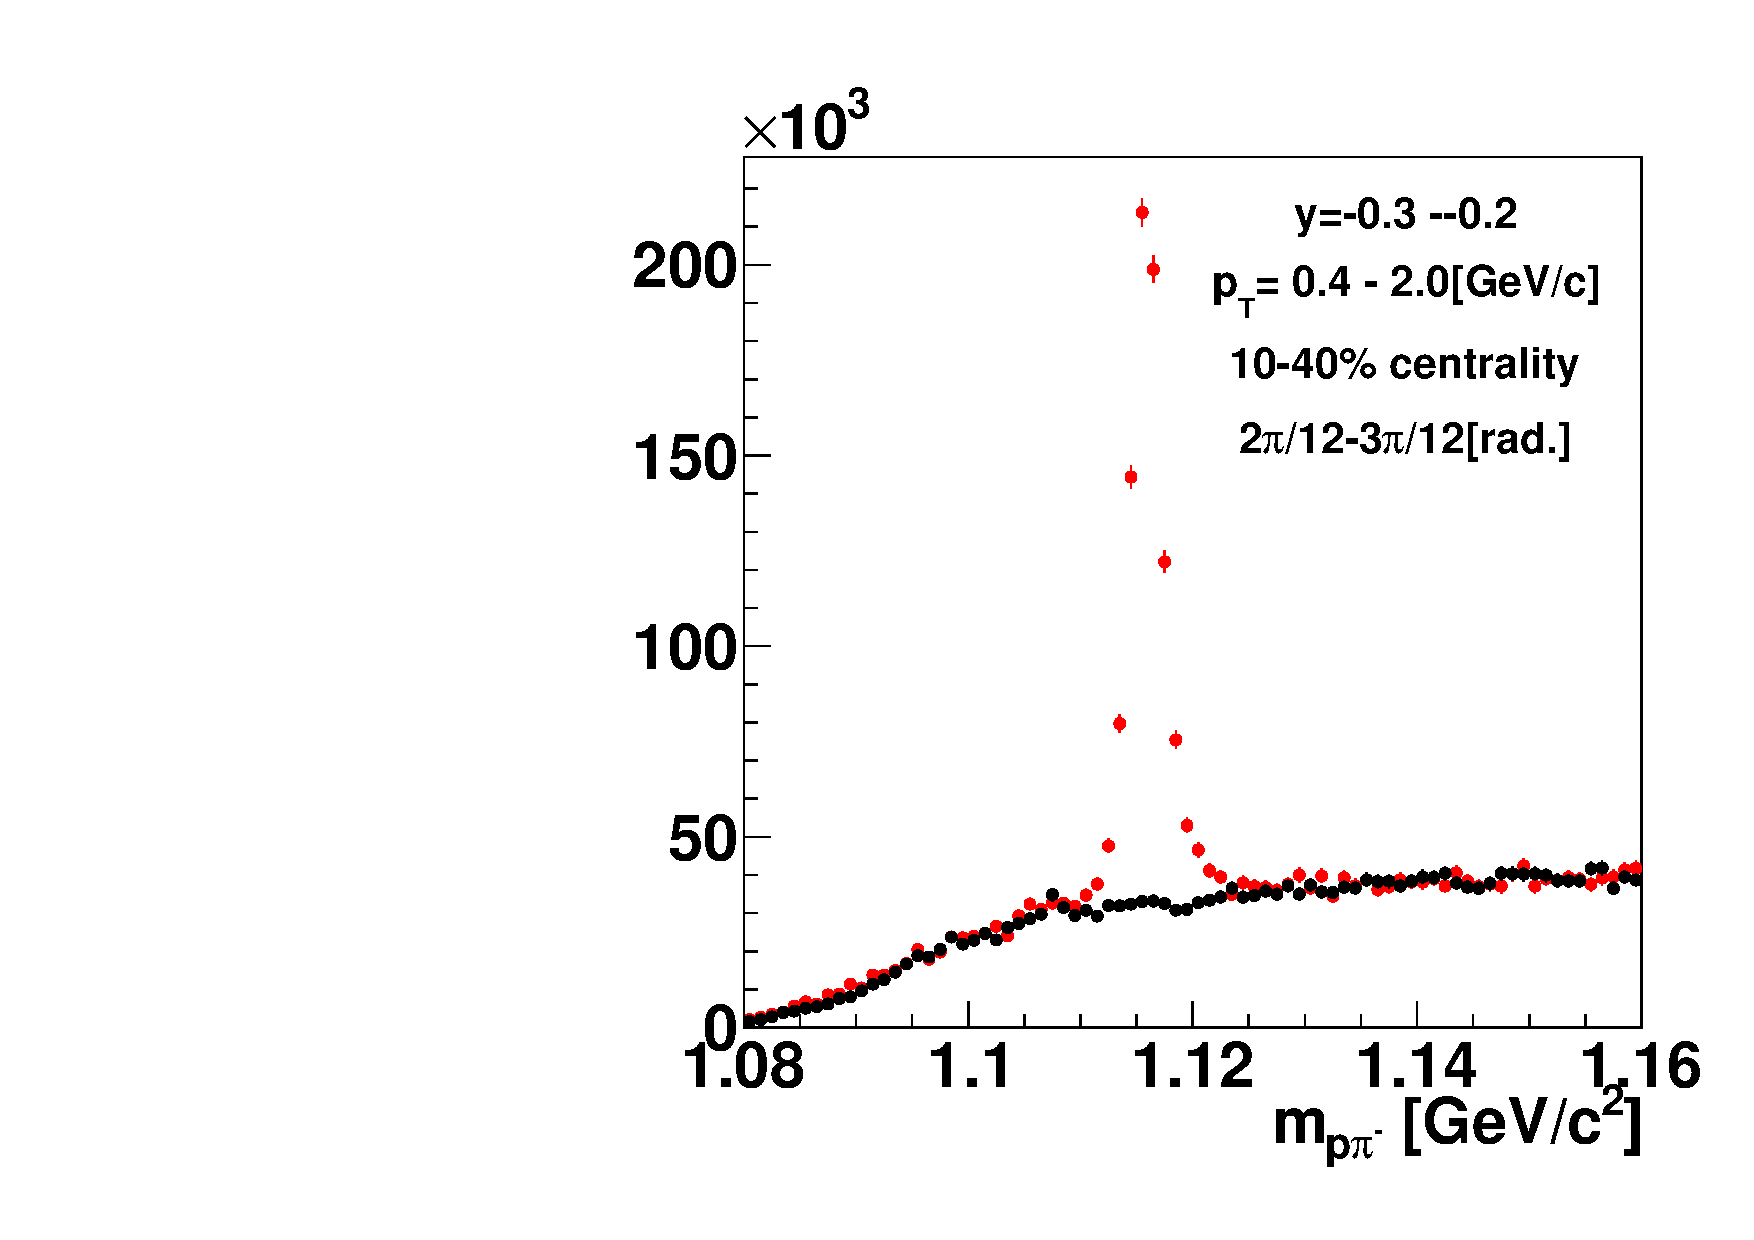
\includegraphics[width=0.14\linewidth]{chapterX/fig/ld_v1_sig/kf_ptslice0_cent1_ld_flow_phi3_rap7_check.pdf}
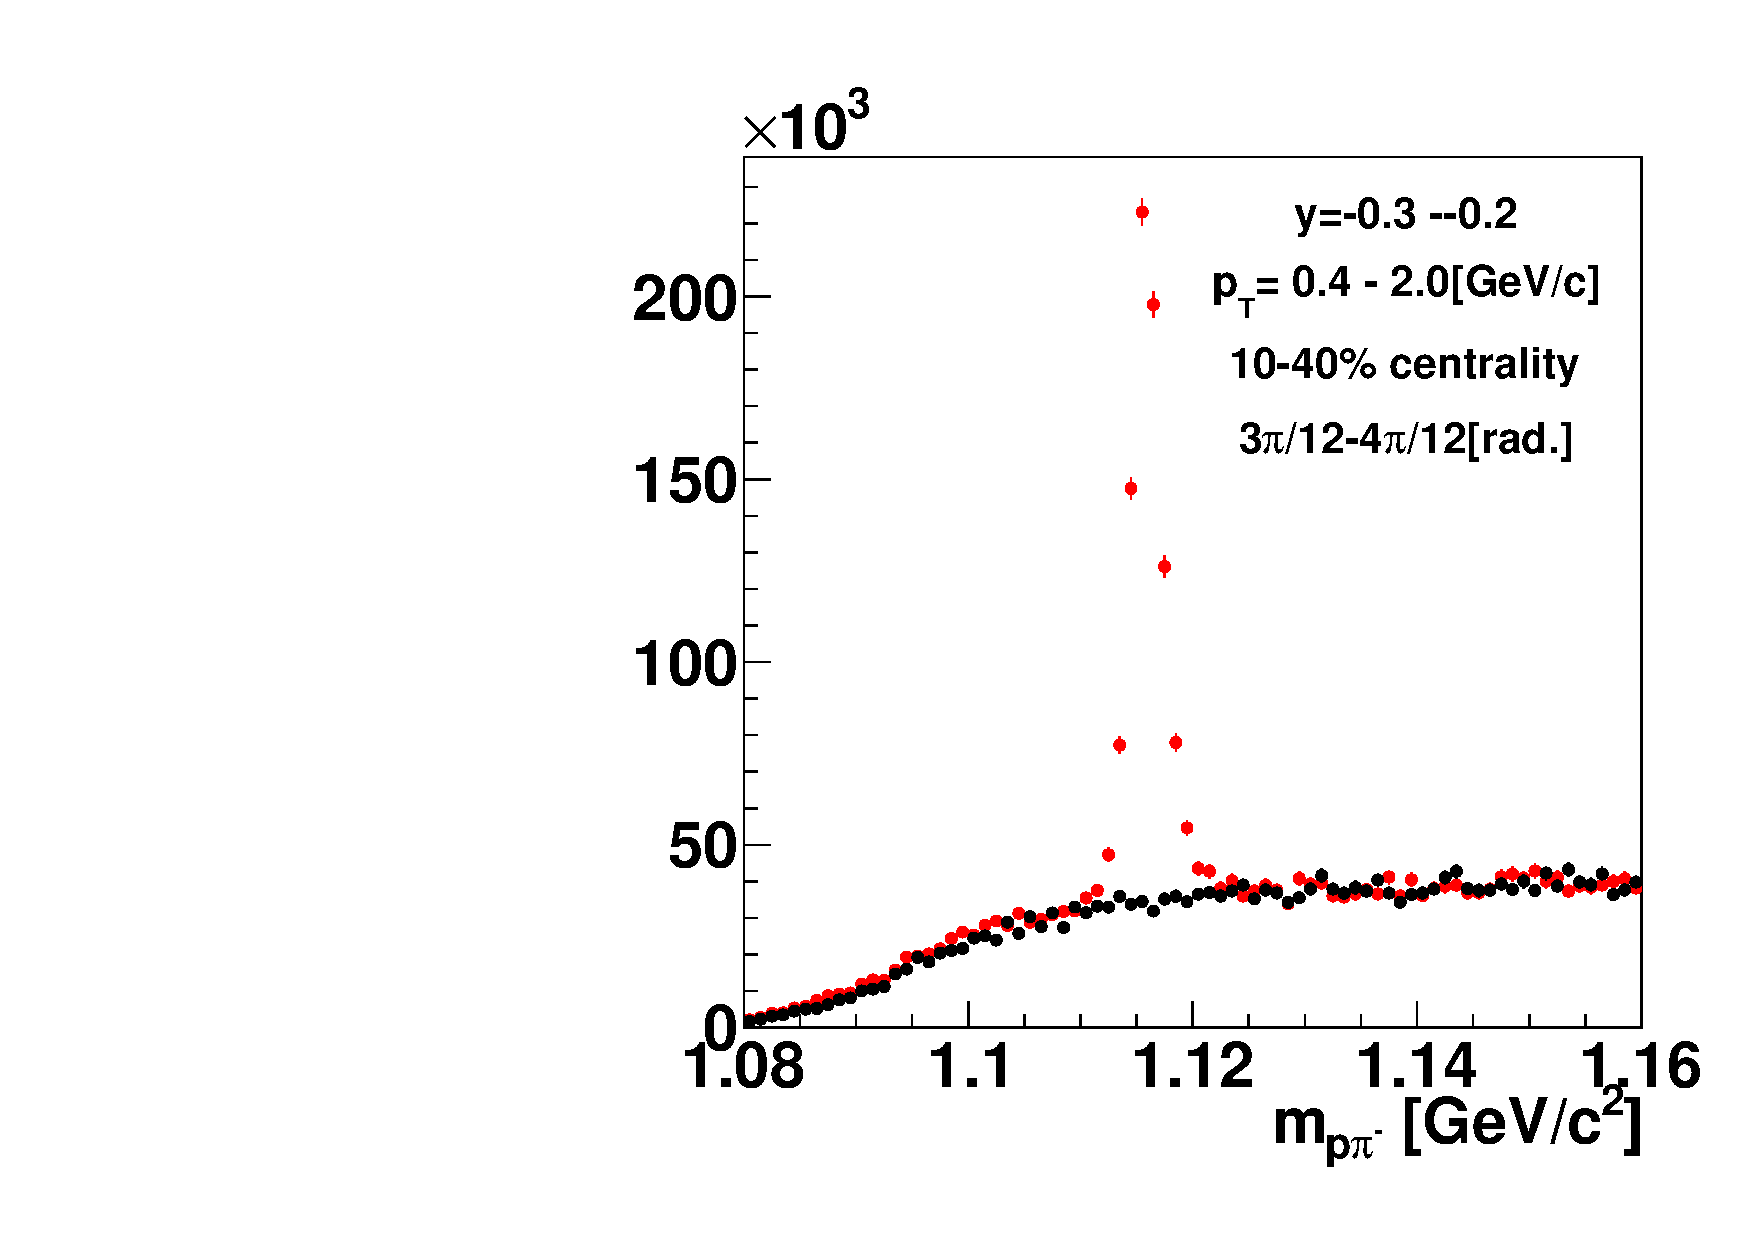
\includegraphics[width=0.14\linewidth]{chapterX/fig/ld_v1_sig/kf_ptslice0_cent1_ld_flow_phi4_rap7_check.pdf}
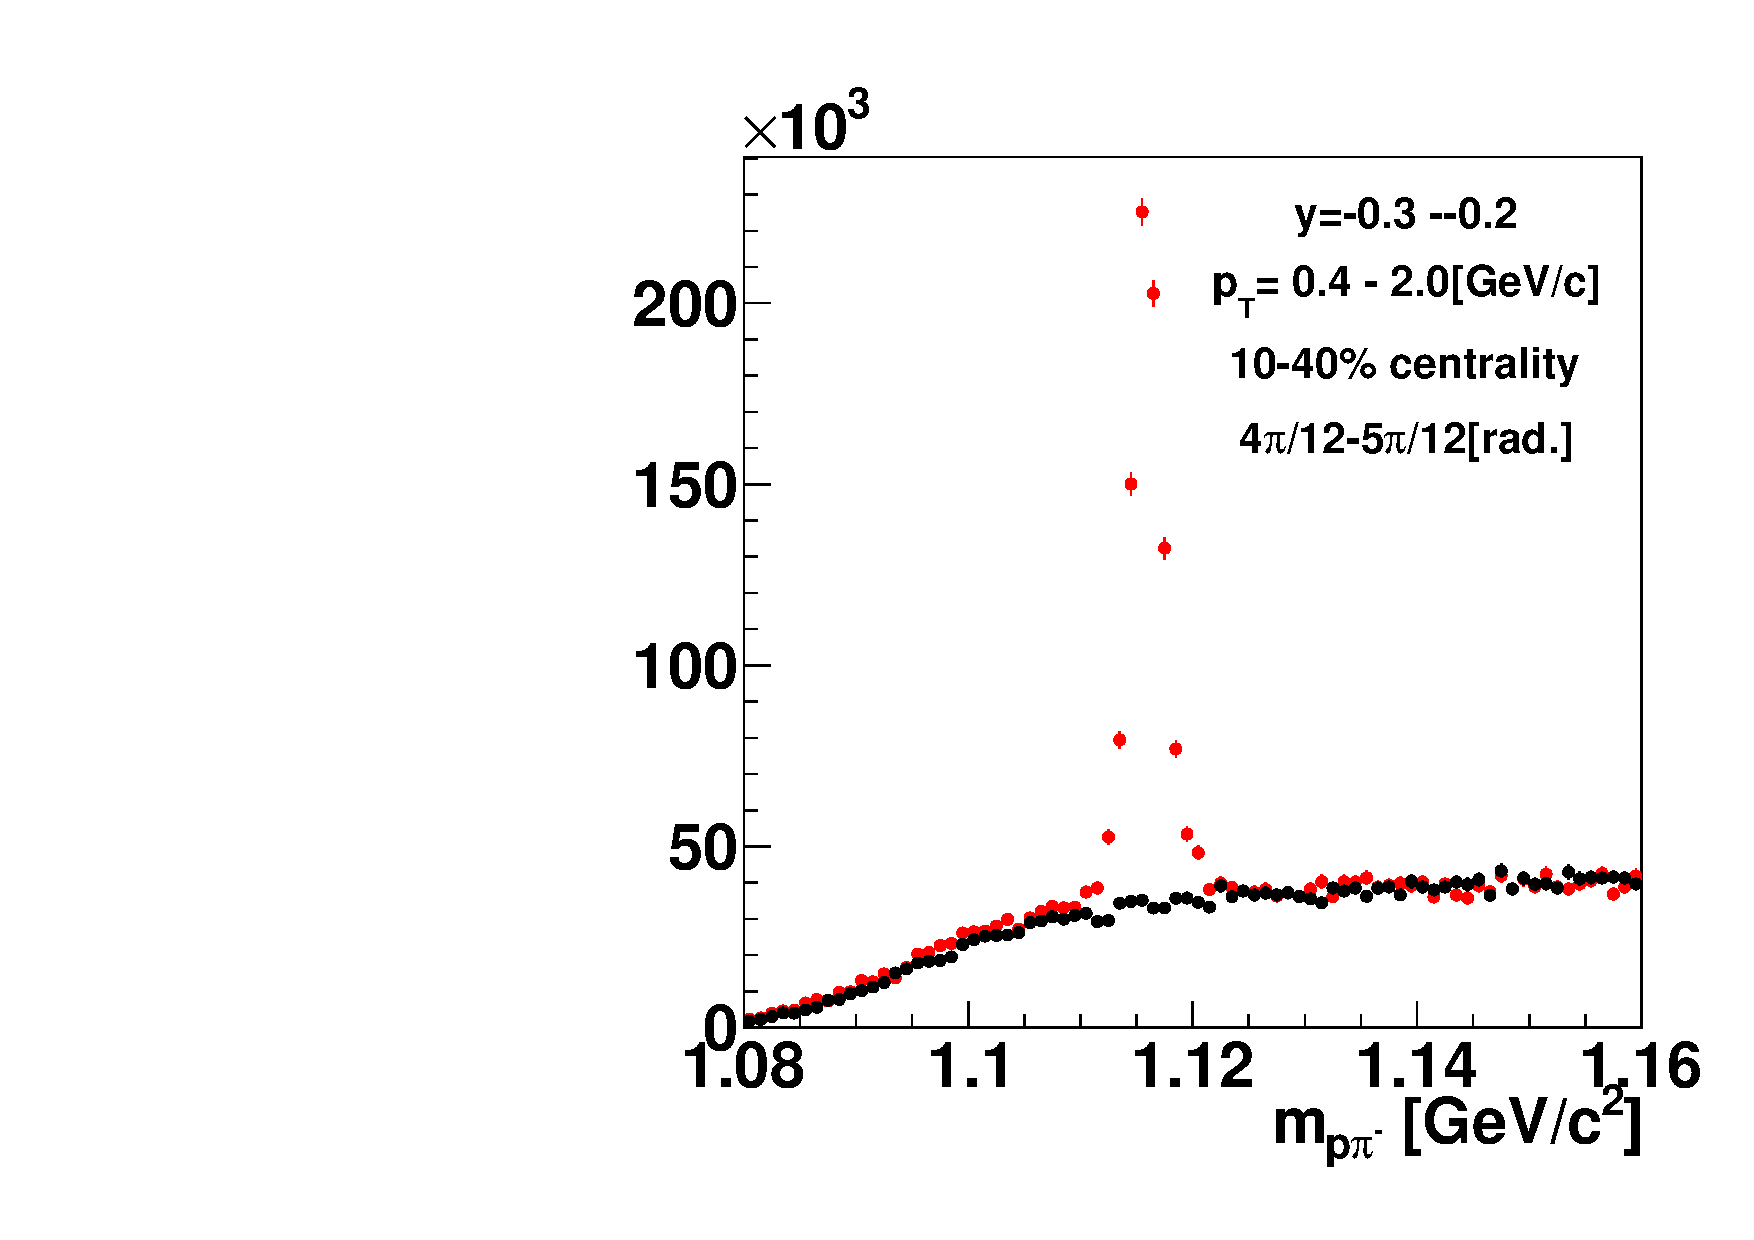
\includegraphics[width=0.14\linewidth]{chapterX/fig/ld_v1_sig/kf_ptslice0_cent1_ld_flow_phi5_rap7_check.pdf}
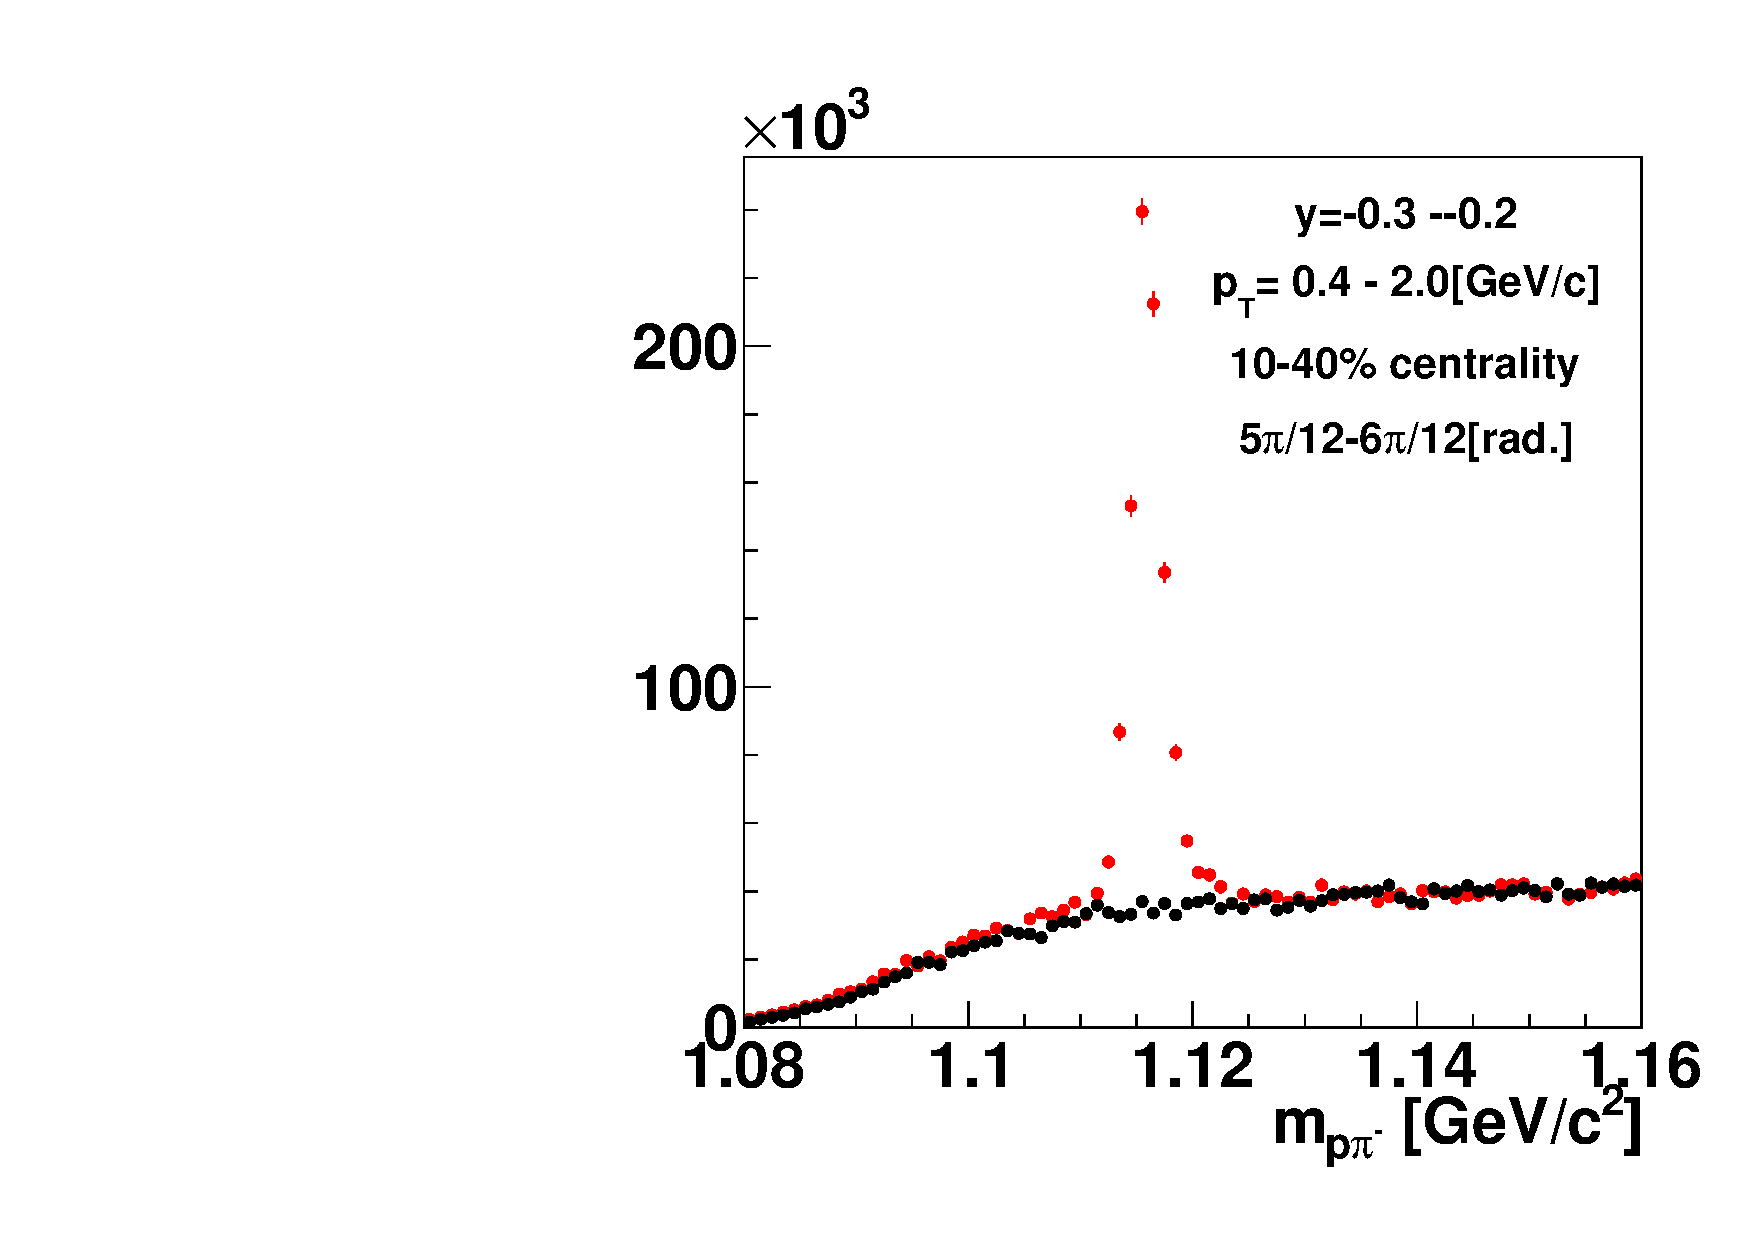
\includegraphics[width=0.14\linewidth]{chapterX/fig/ld_v1_sig/kf_ptslice0_cent1_ld_flow_phi6_rap7_check.pdf}
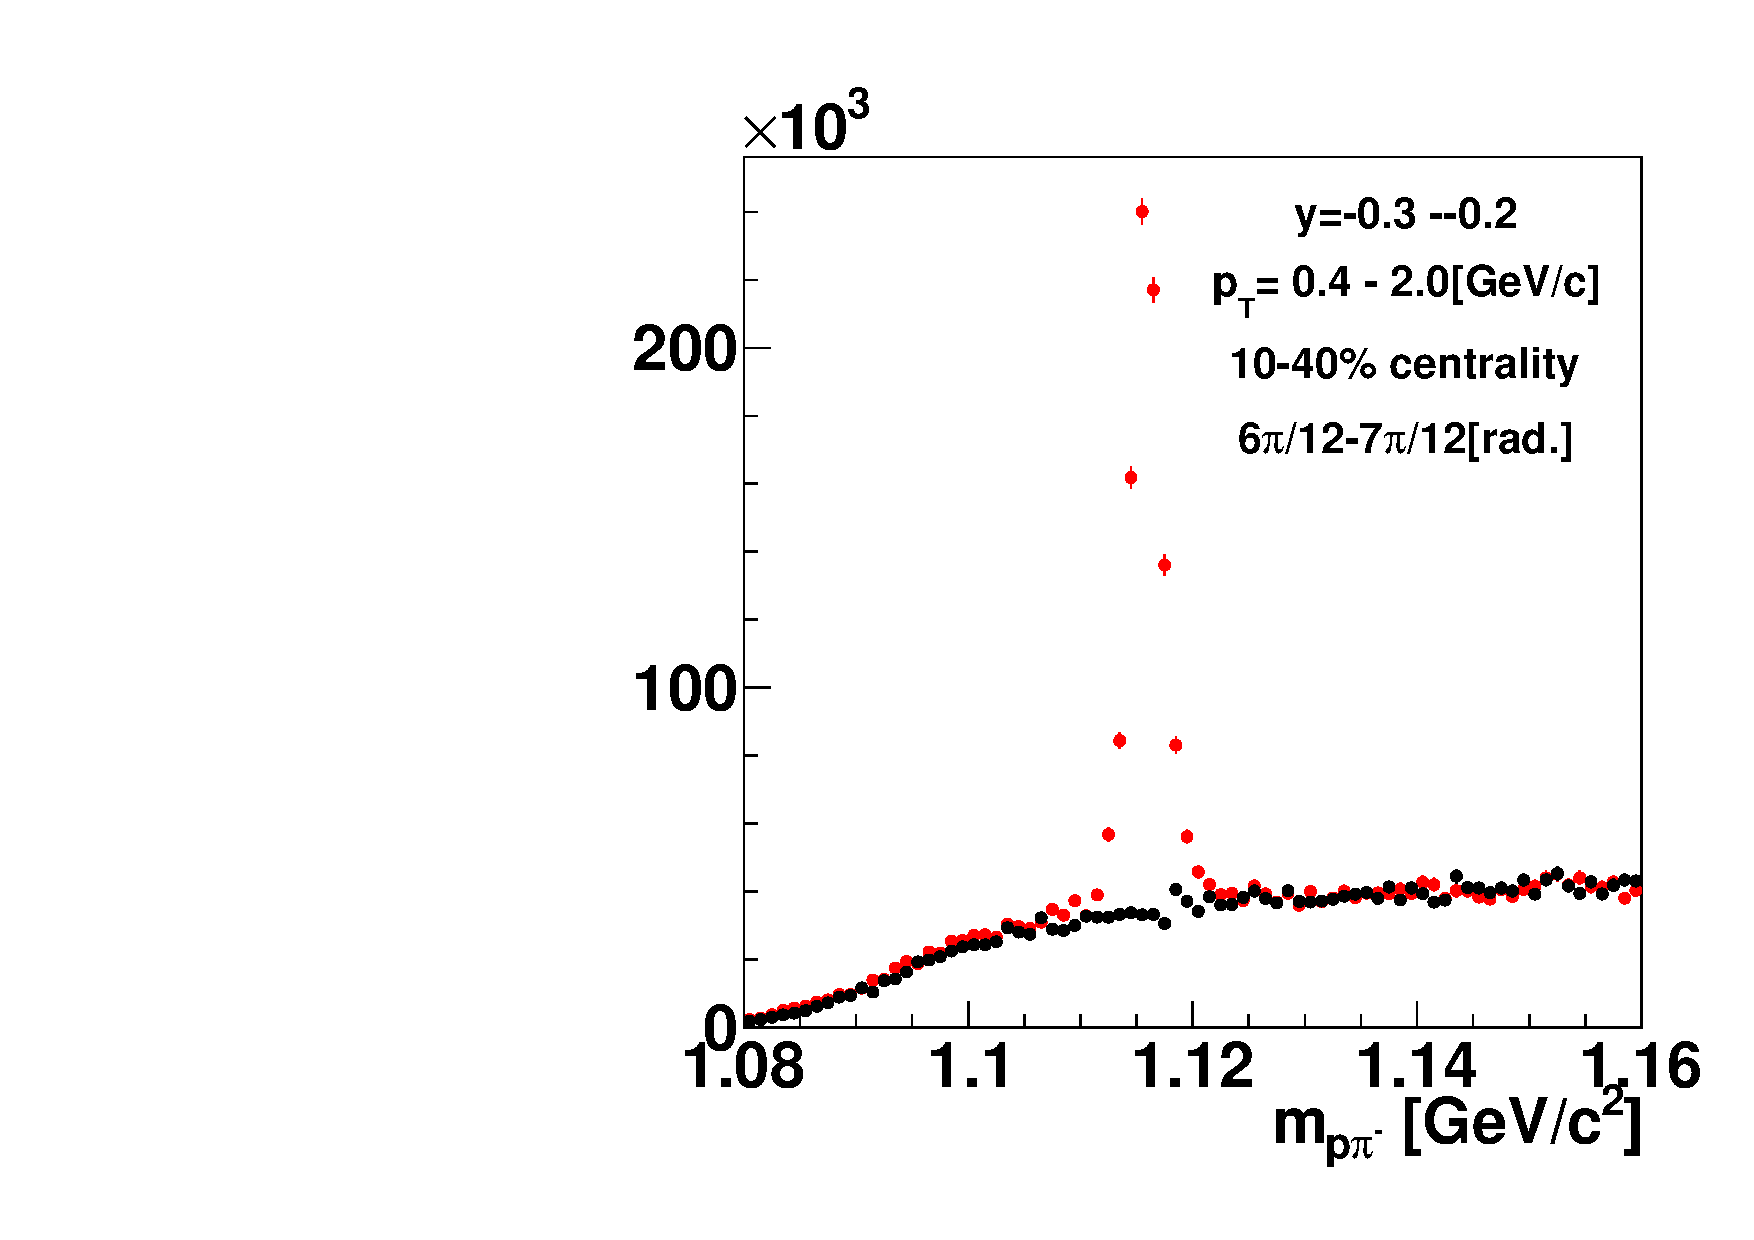
\includegraphics[width=0.14\linewidth]{chapterX/fig/ld_v1_sig/kf_ptslice0_cent1_ld_flow_phi7_rap7_check.pdf}
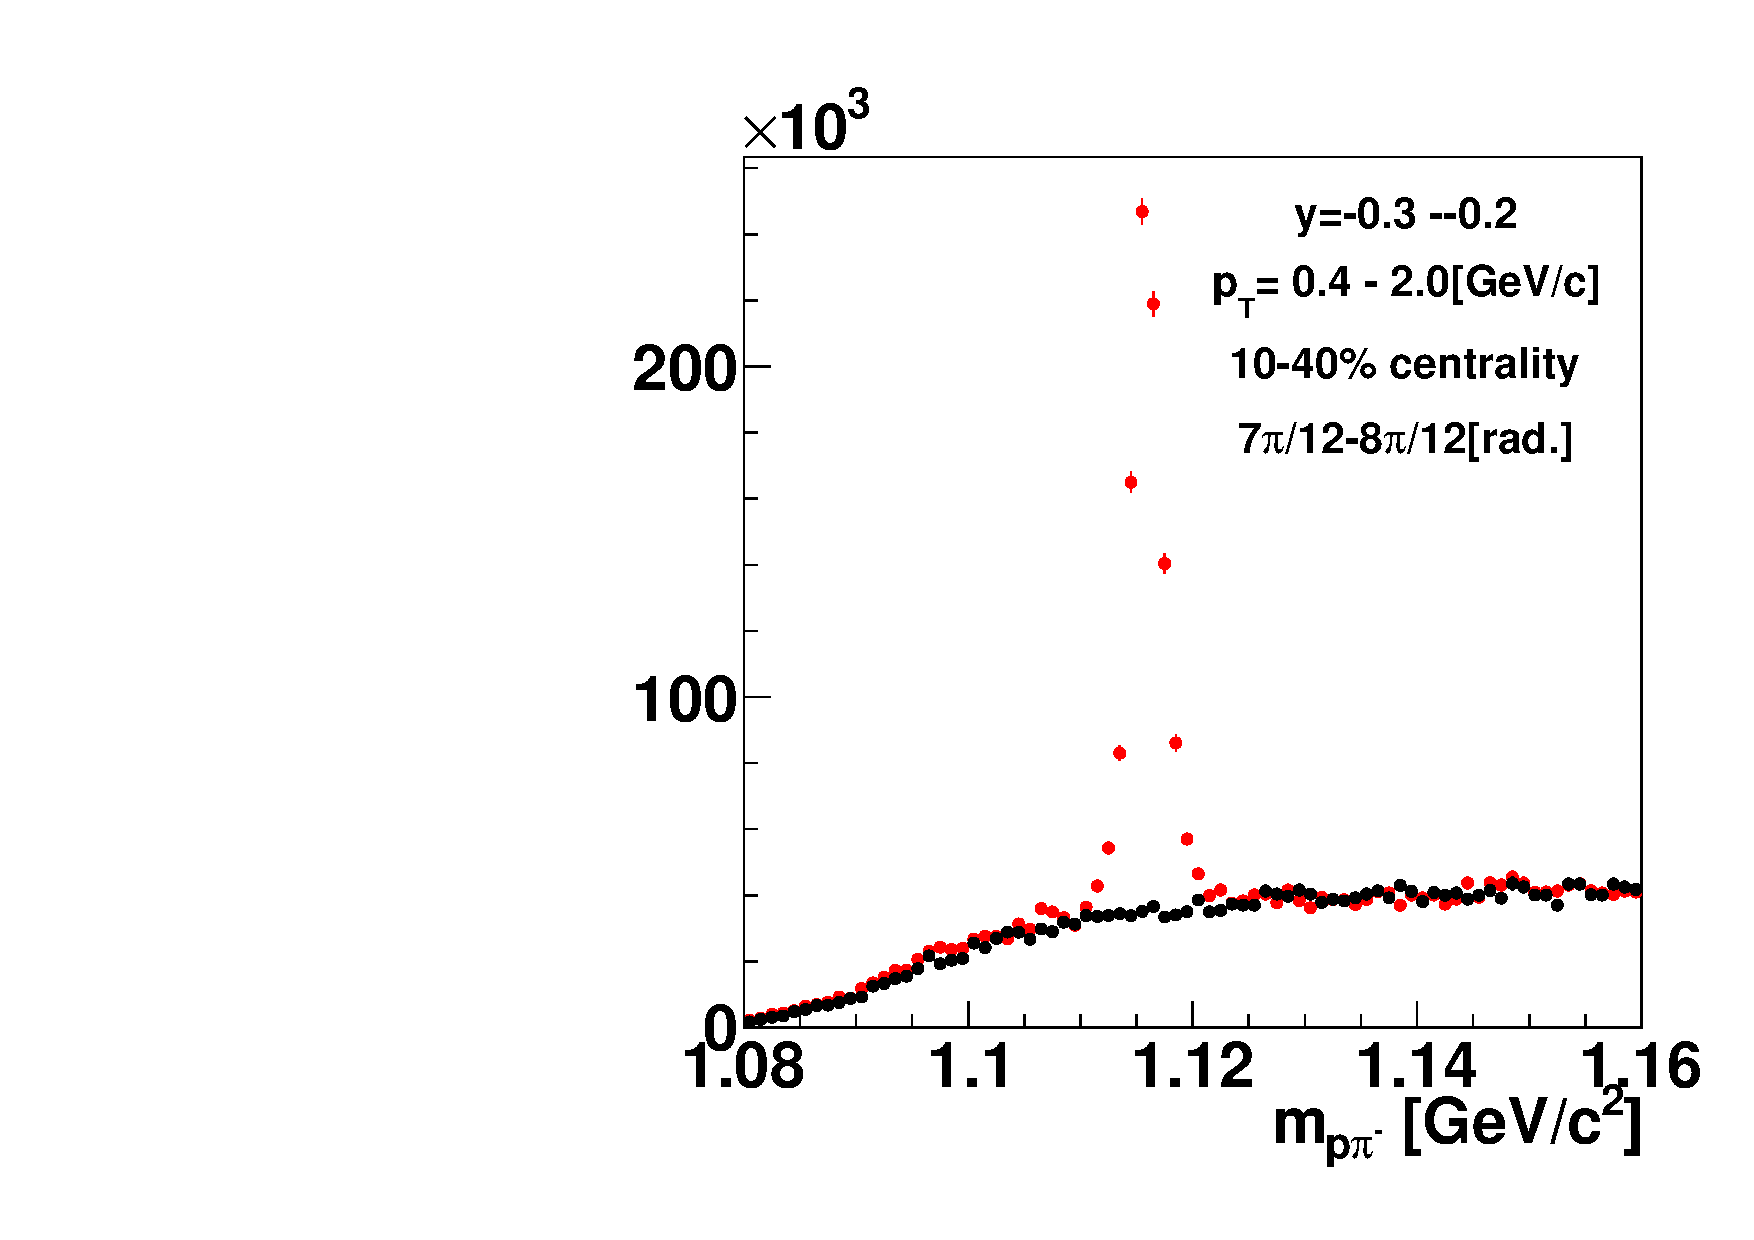
\includegraphics[width=0.14\linewidth]{chapterX/fig/ld_v1_sig/kf_ptslice0_cent1_ld_flow_phi8_rap7_check.pdf}
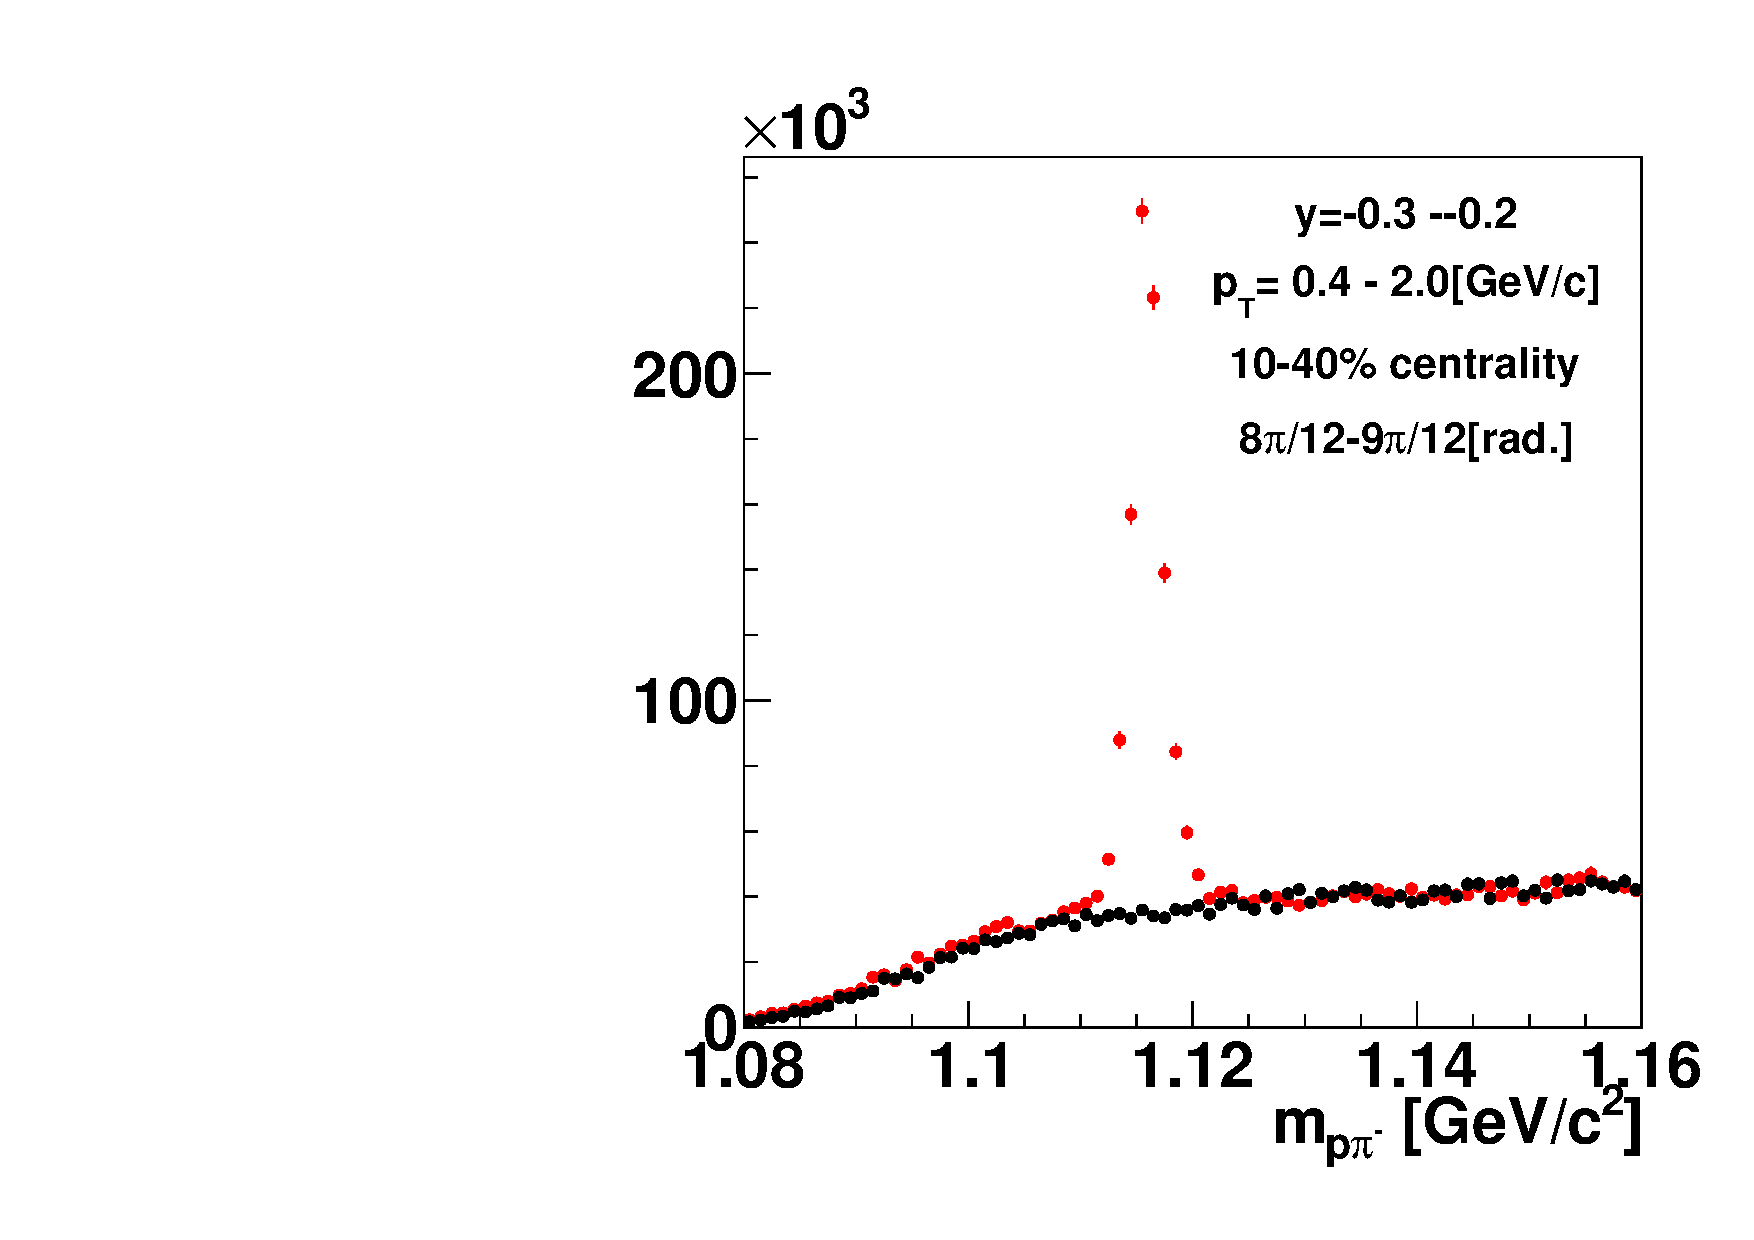
\includegraphics[width=0.14\linewidth]{chapterX/fig/ld_v1_sig/kf_ptslice0_cent1_ld_flow_phi9_rap7_check.pdf}
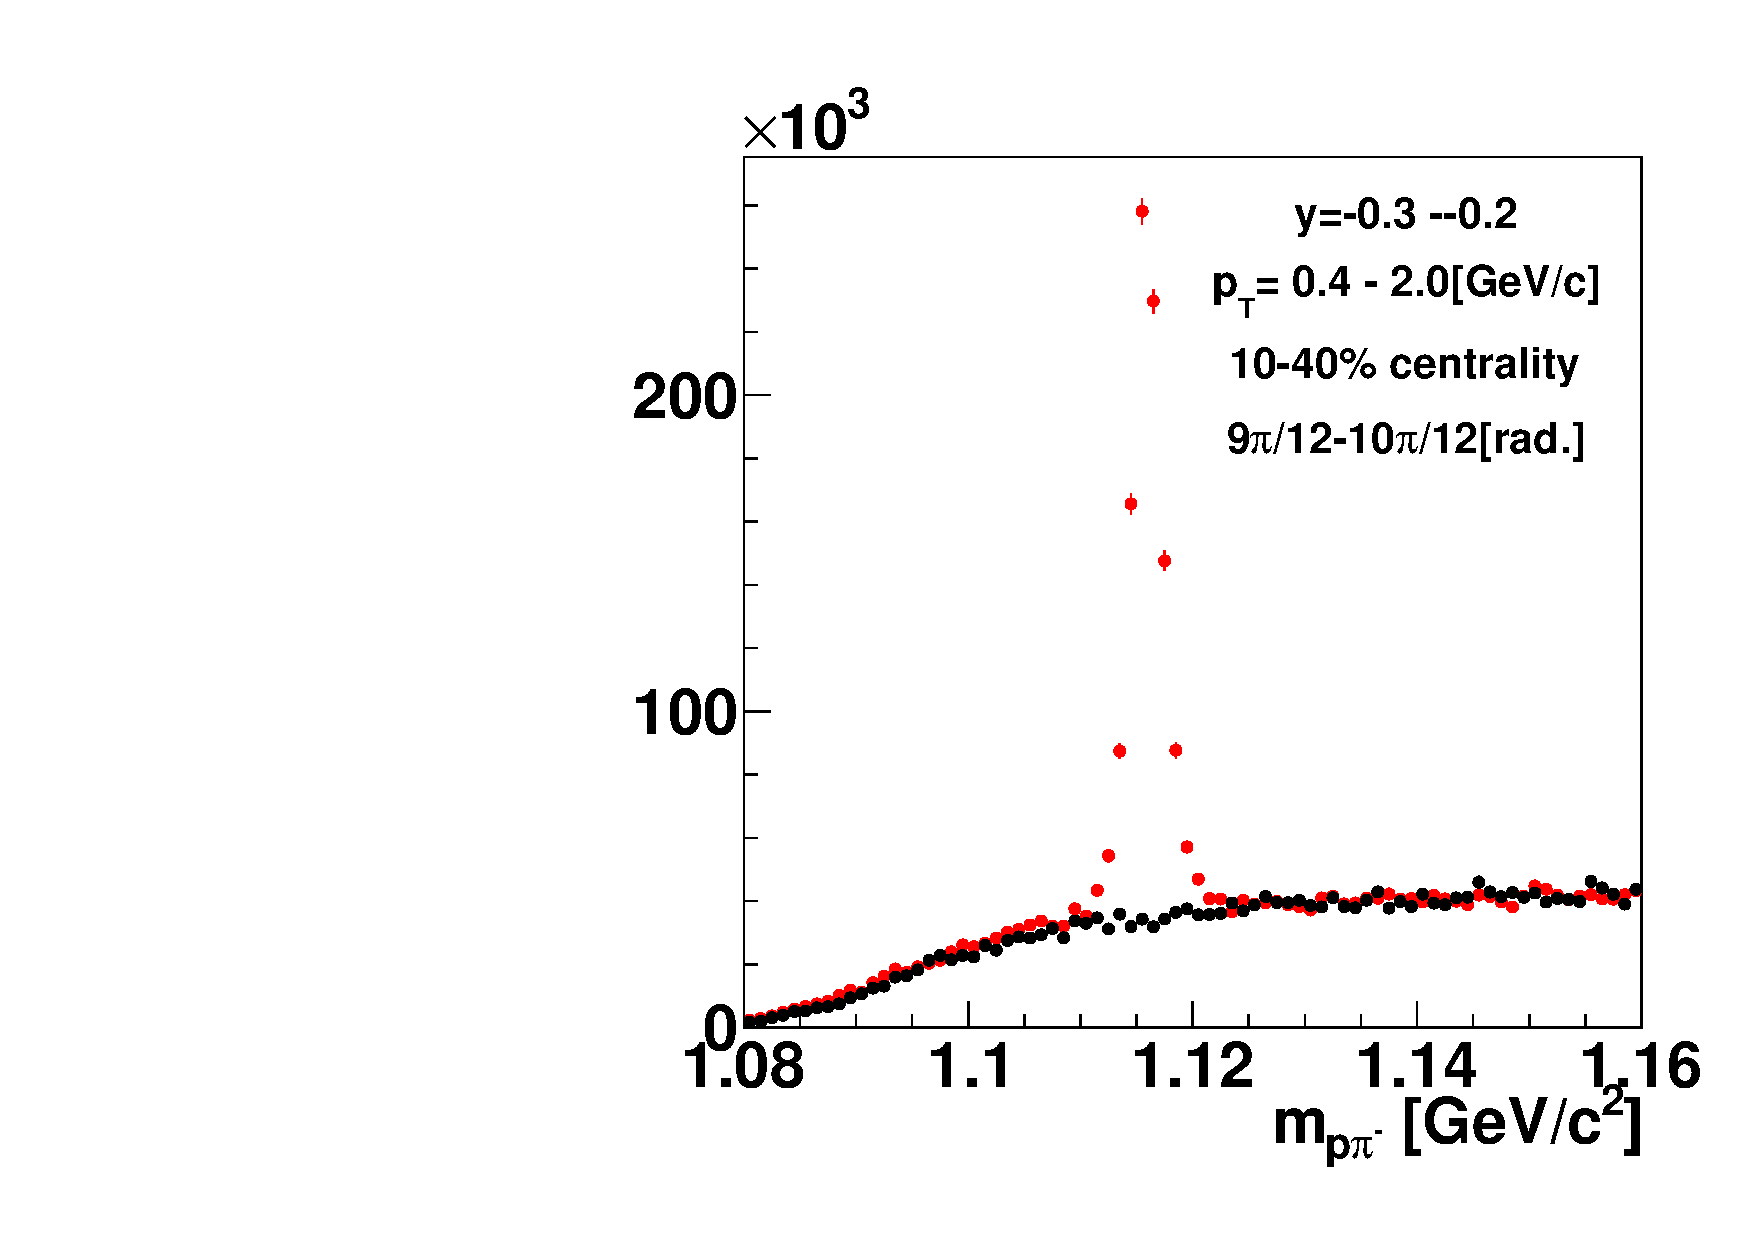
\includegraphics[width=0.14\linewidth]{chapterX/fig/ld_v1_sig/kf_ptslice0_cent1_ld_flow_phi10_rap7_check.pdf}
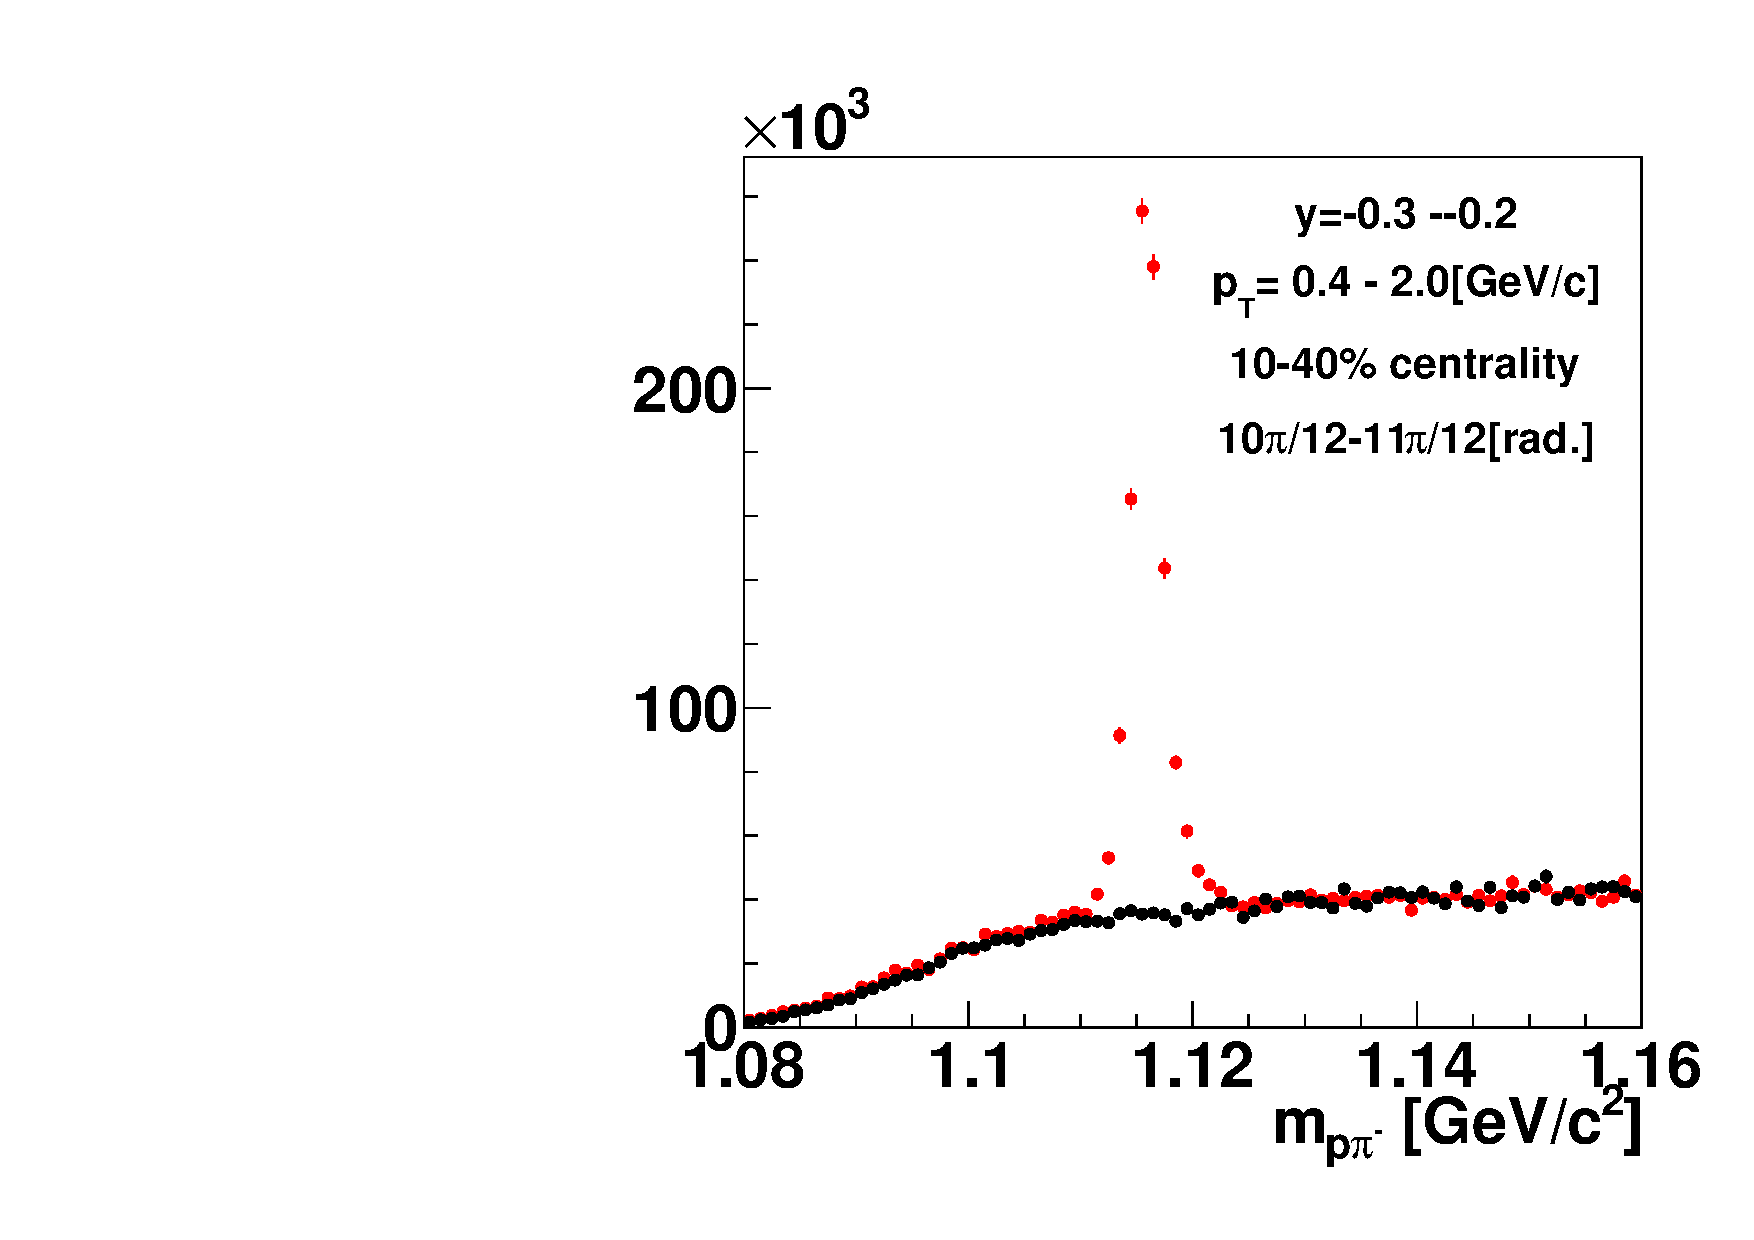
\includegraphics[width=0.14\linewidth]{chapterX/fig/ld_v1_sig/kf_ptslice0_cent1_ld_flow_phi11_rap7_check.pdf}
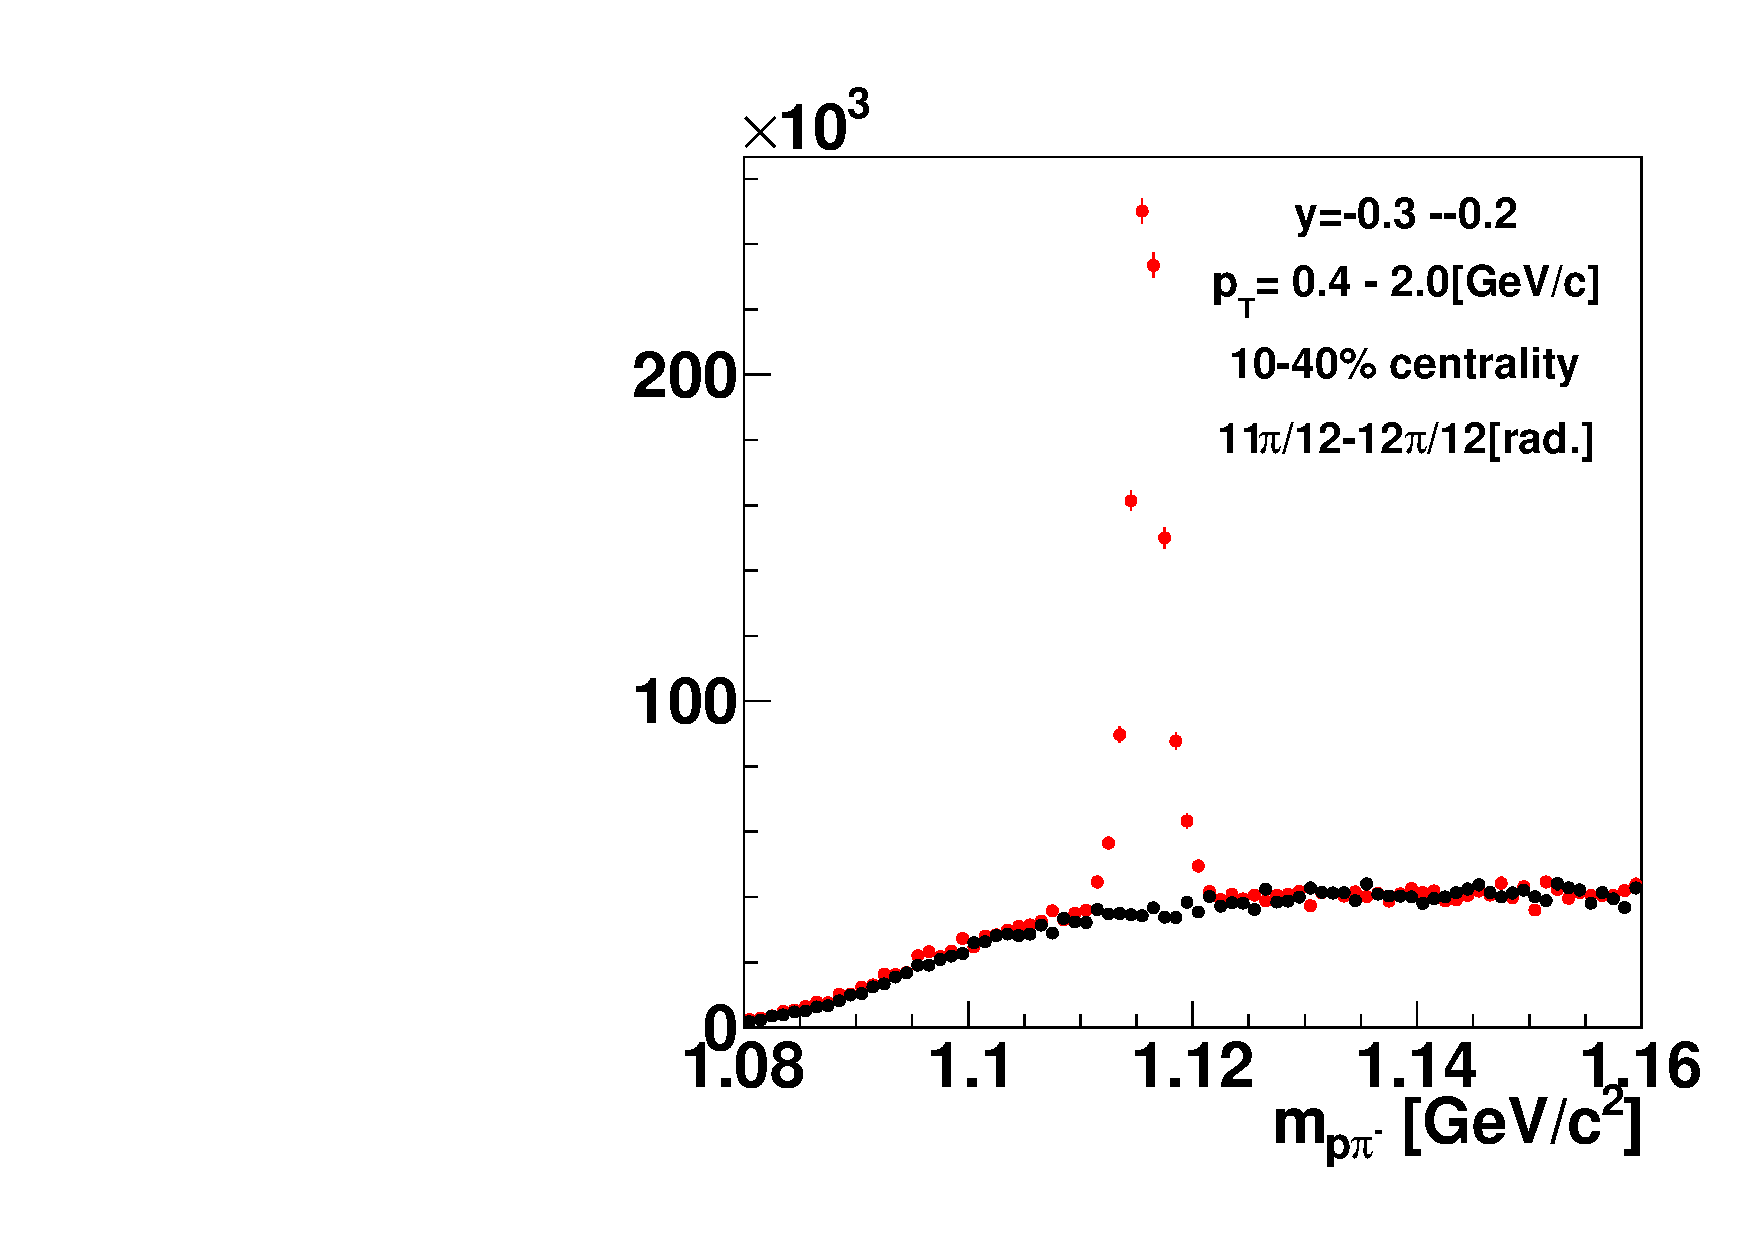
\includegraphics[width=0.14\linewidth]{chapterX/fig/ld_v1_sig/kf_ptslice0_cent1_ld_flow_phi12_rap7_check.pdf}

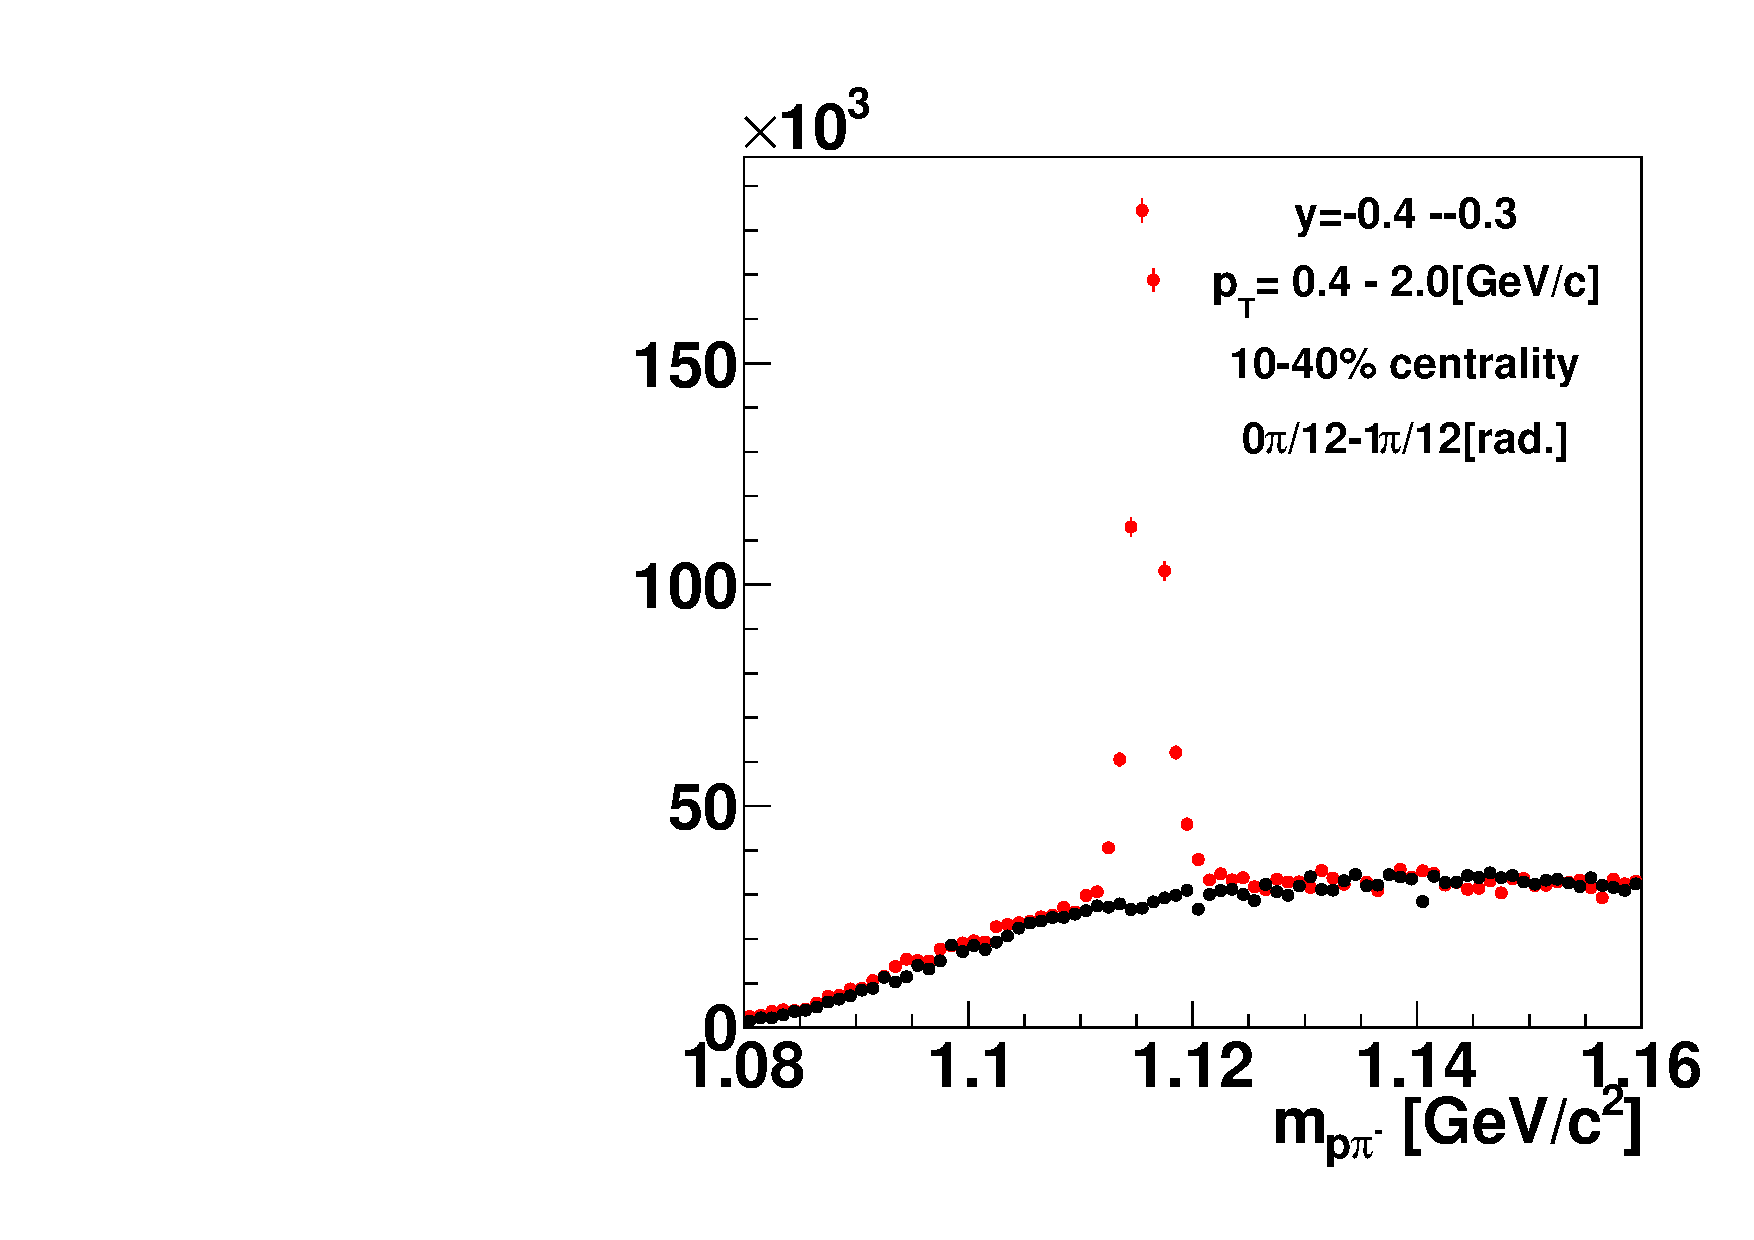
\includegraphics[width=0.14\linewidth]{chapterX/fig/ld_v1_sig/kf_ptslice0_cent1_ld_flow_phi1_rap8_check.pdf}
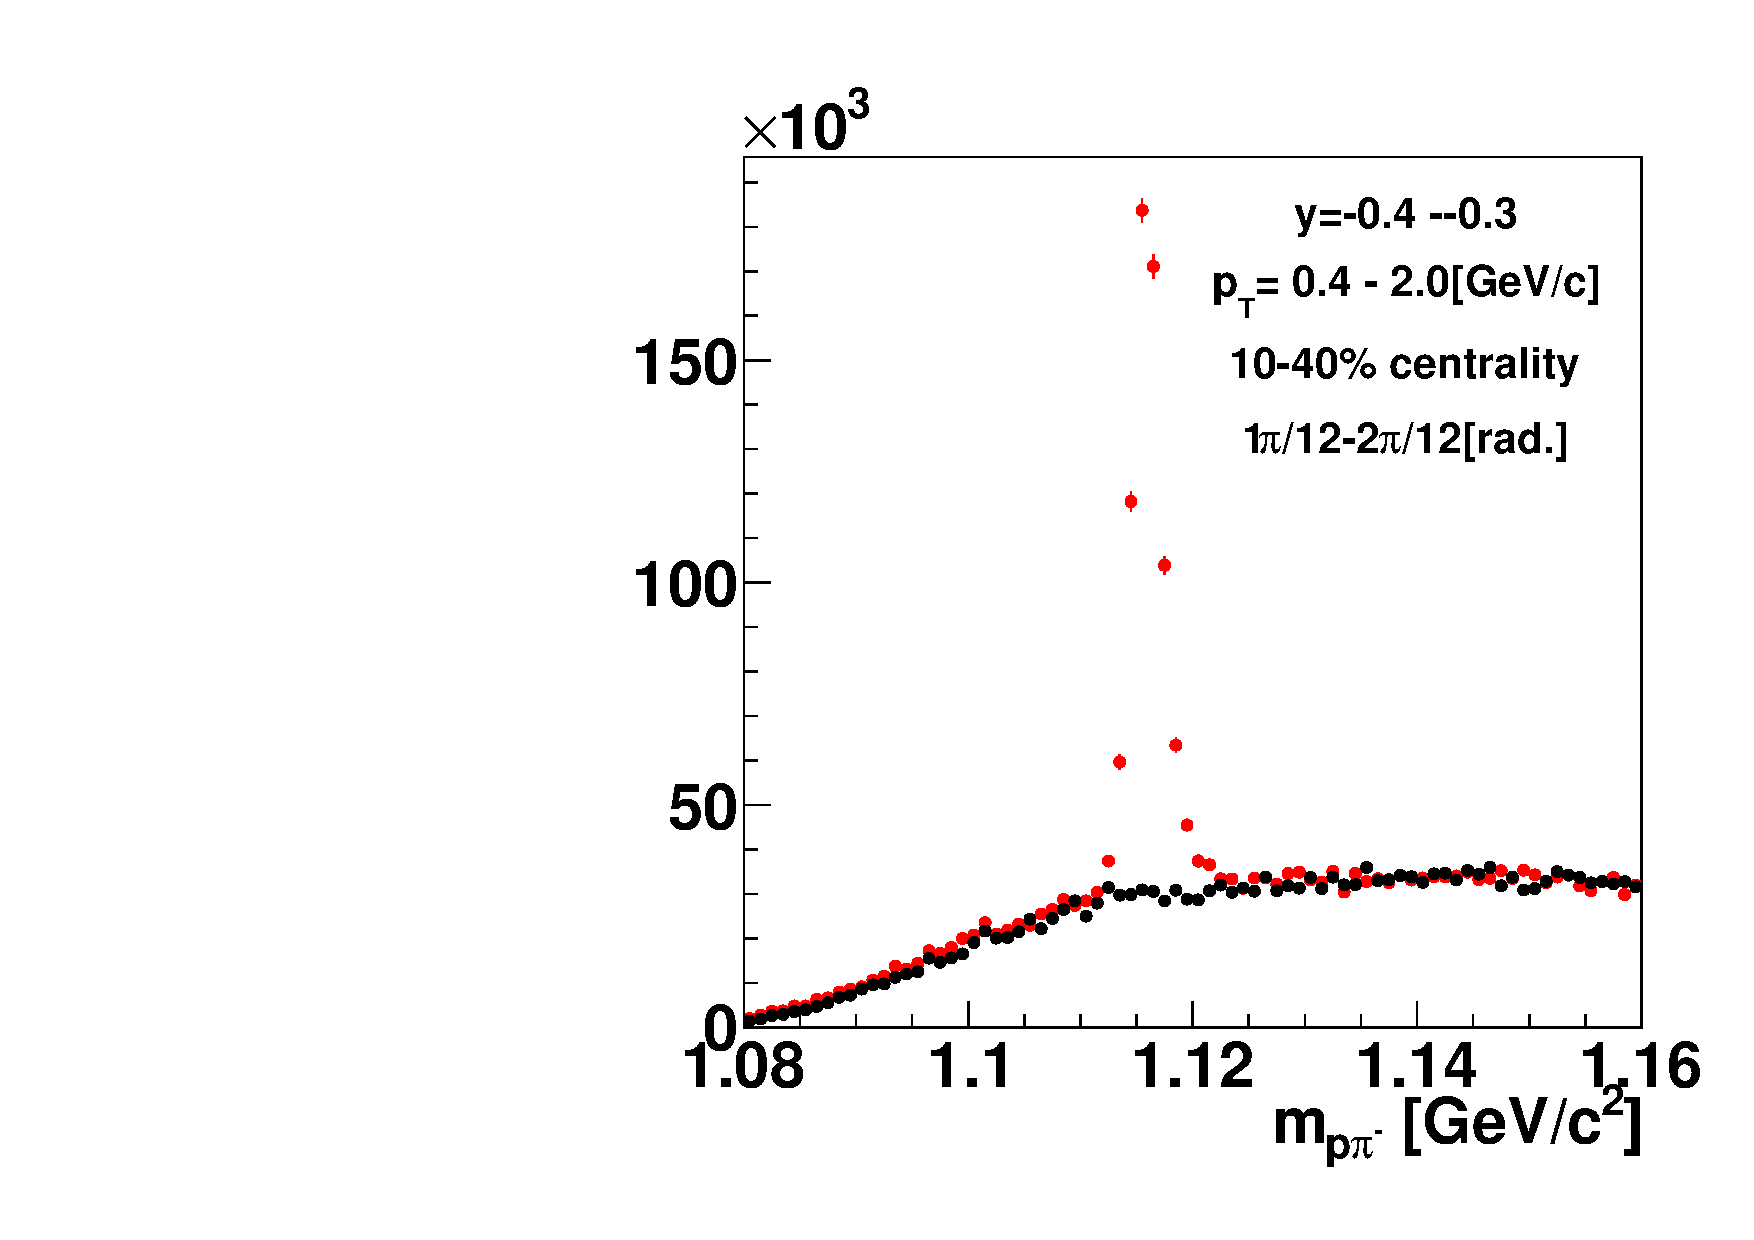
\includegraphics[width=0.14\linewidth]{chapterX/fig/ld_v1_sig/kf_ptslice0_cent1_ld_flow_phi2_rap8_check.pdf}
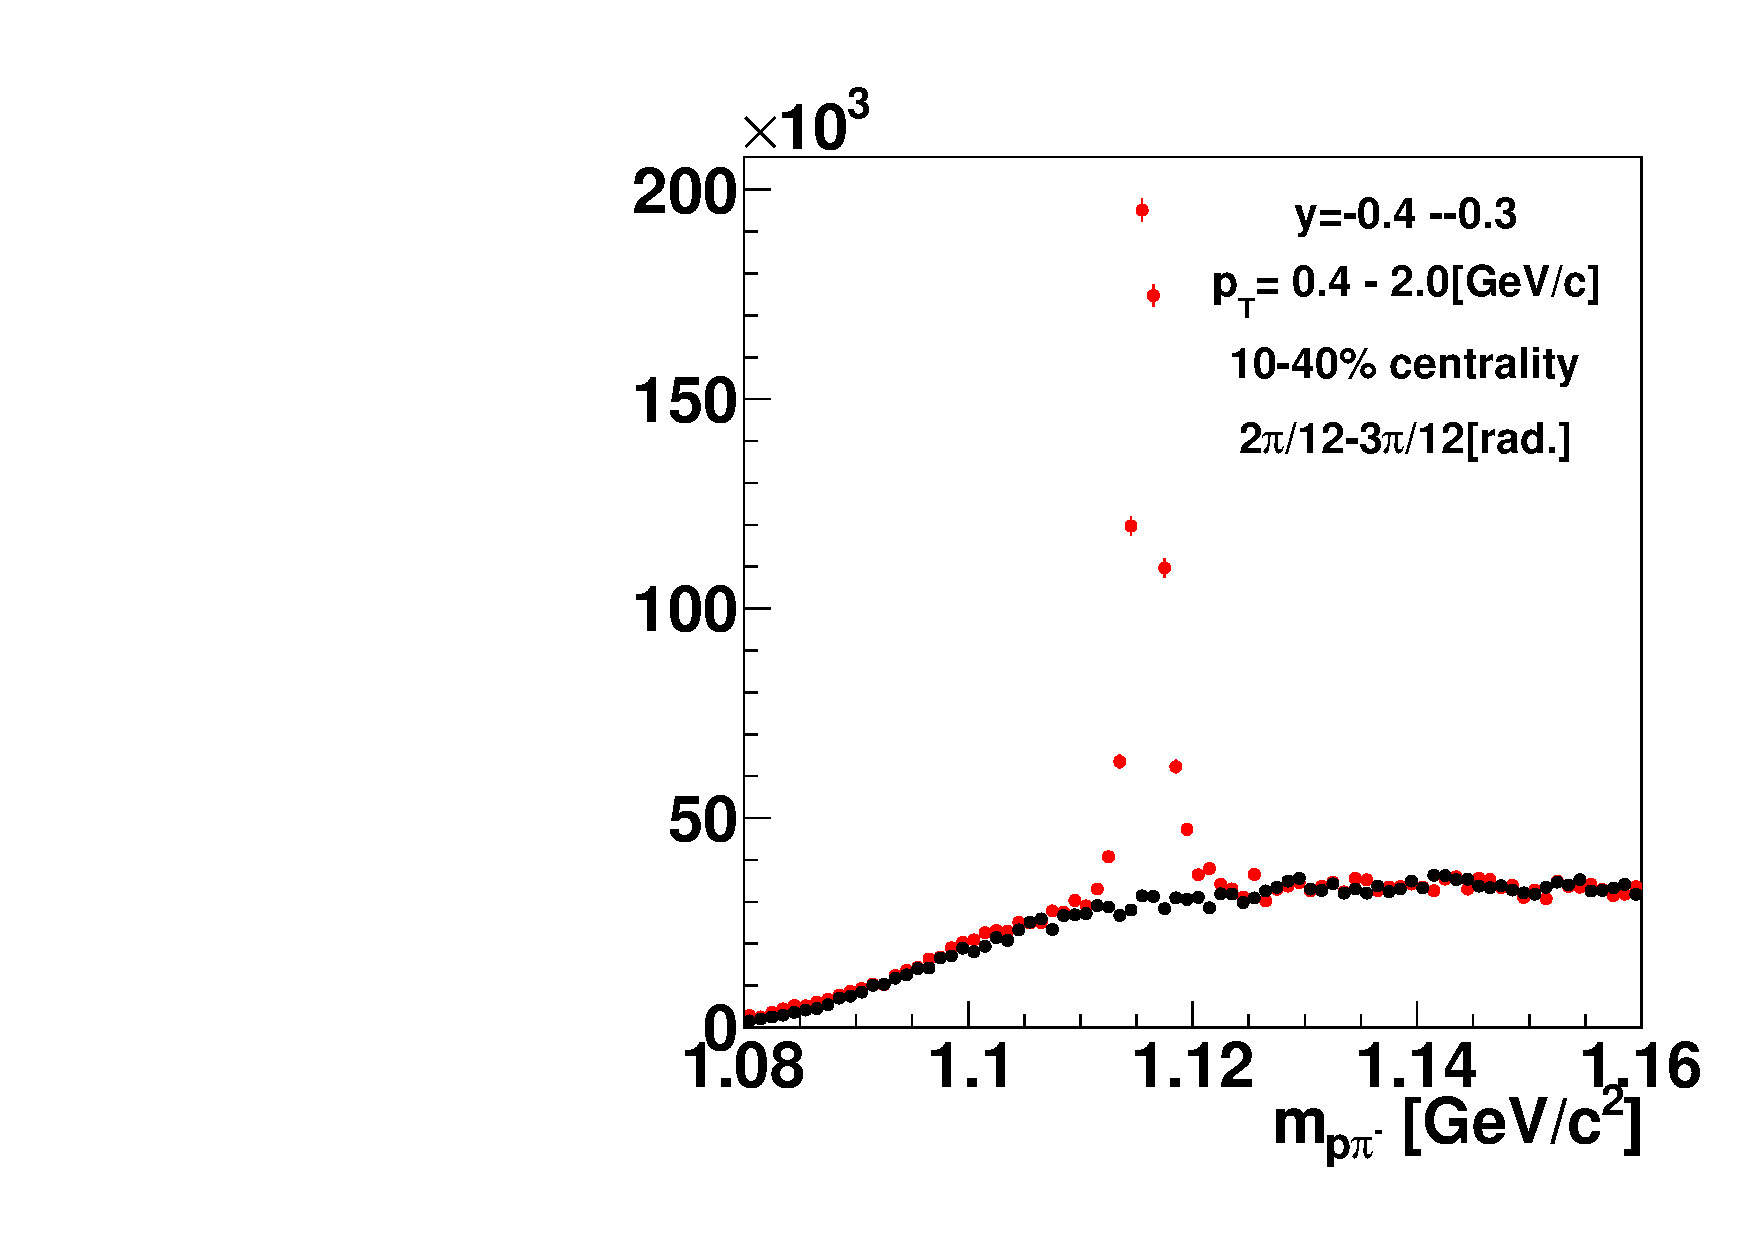
\includegraphics[width=0.14\linewidth]{chapterX/fig/ld_v1_sig/kf_ptslice0_cent1_ld_flow_phi3_rap8_check.pdf}
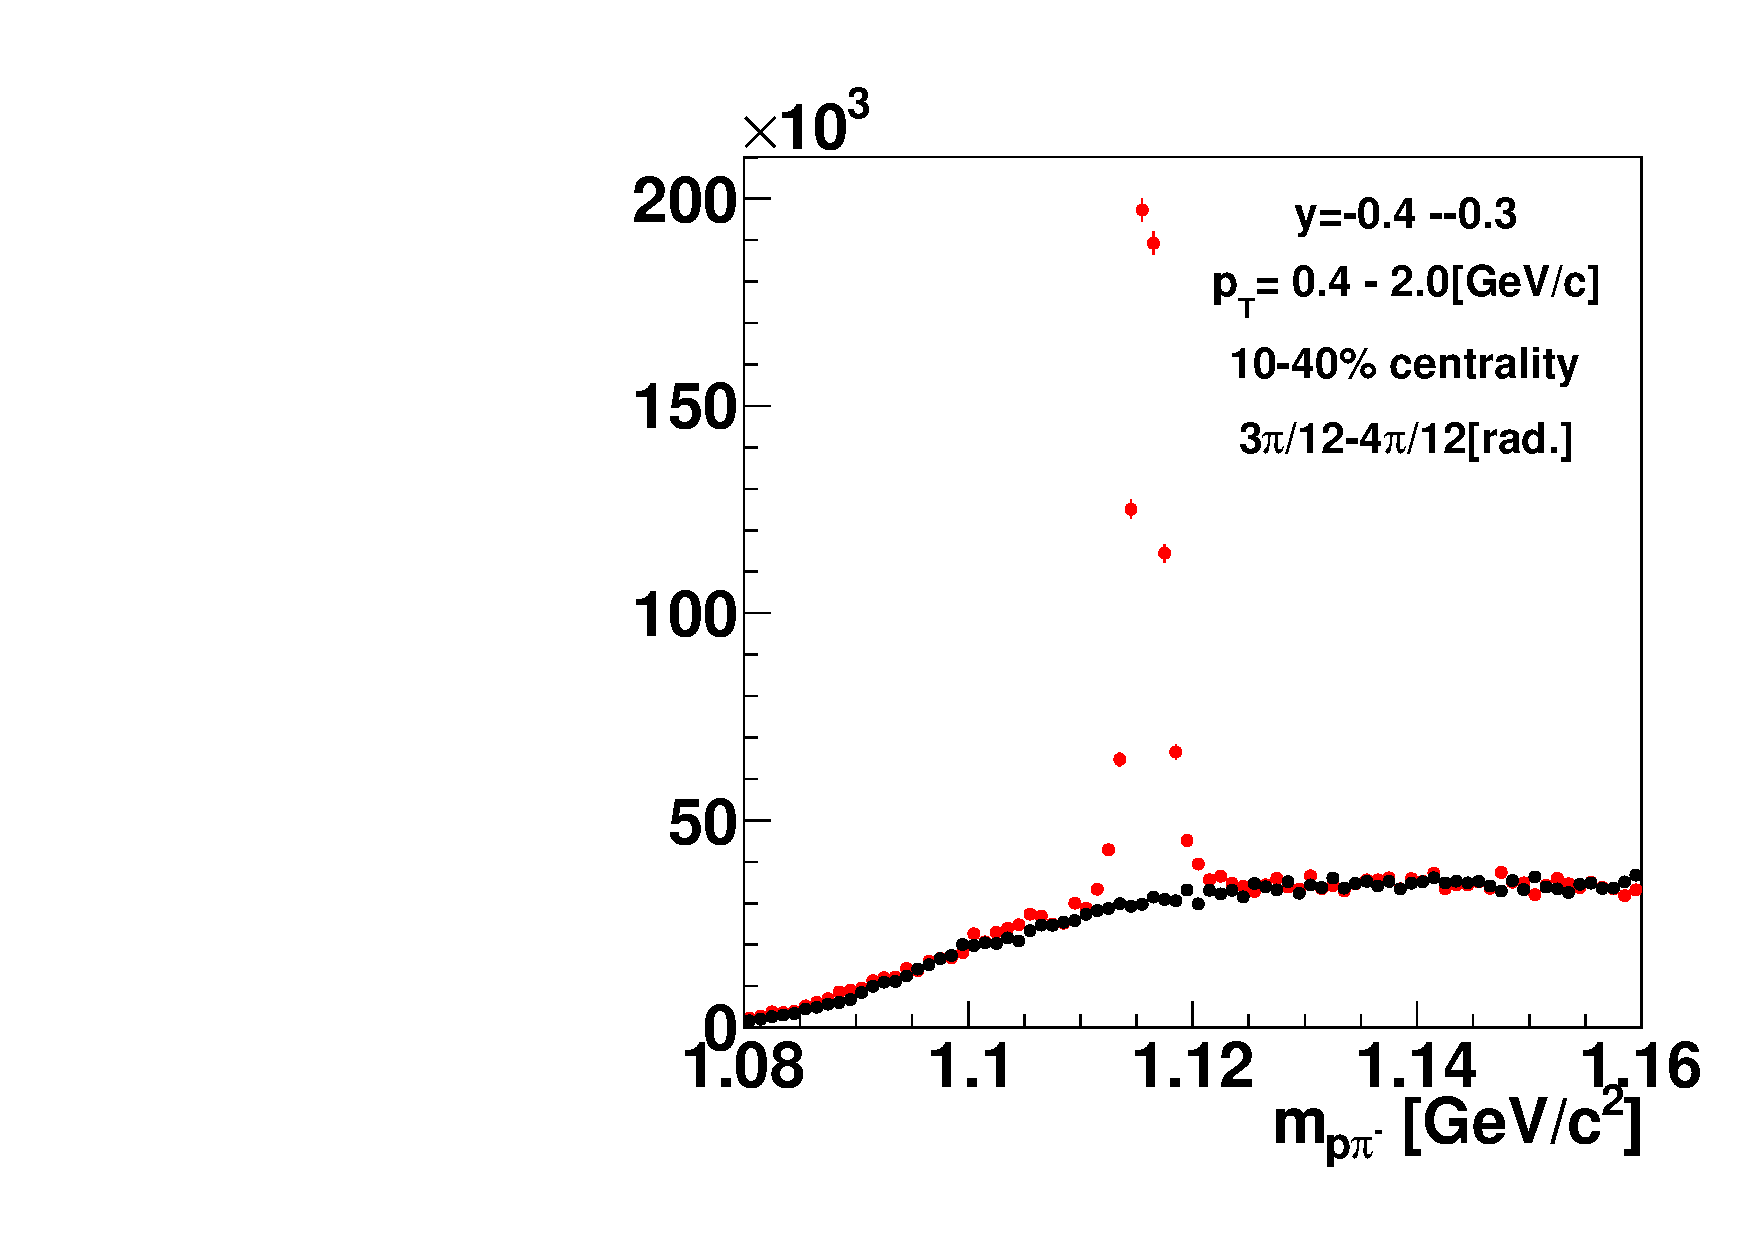
\includegraphics[width=0.14\linewidth]{chapterX/fig/ld_v1_sig/kf_ptslice0_cent1_ld_flow_phi4_rap8_check.pdf}
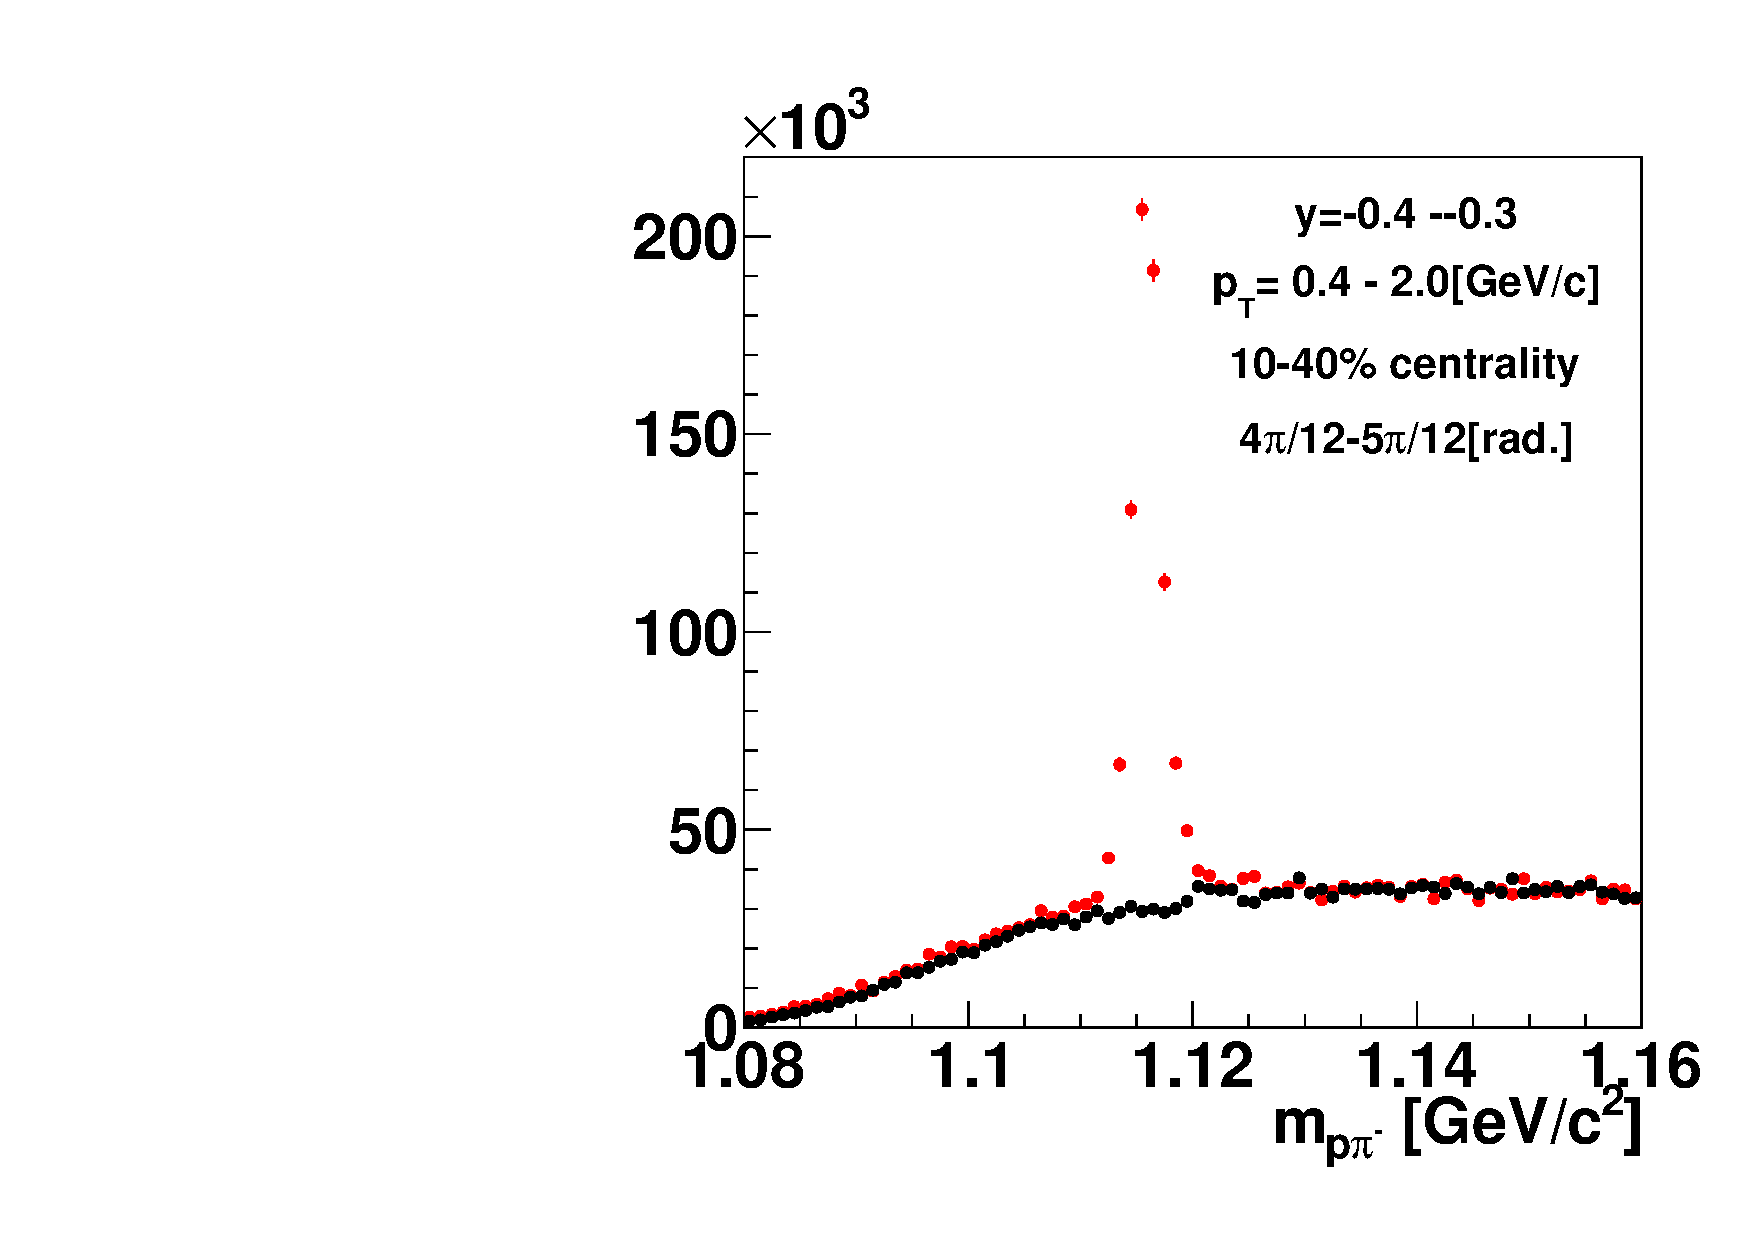
\includegraphics[width=0.14\linewidth]{chapterX/fig/ld_v1_sig/kf_ptslice0_cent1_ld_flow_phi5_rap8_check.pdf}
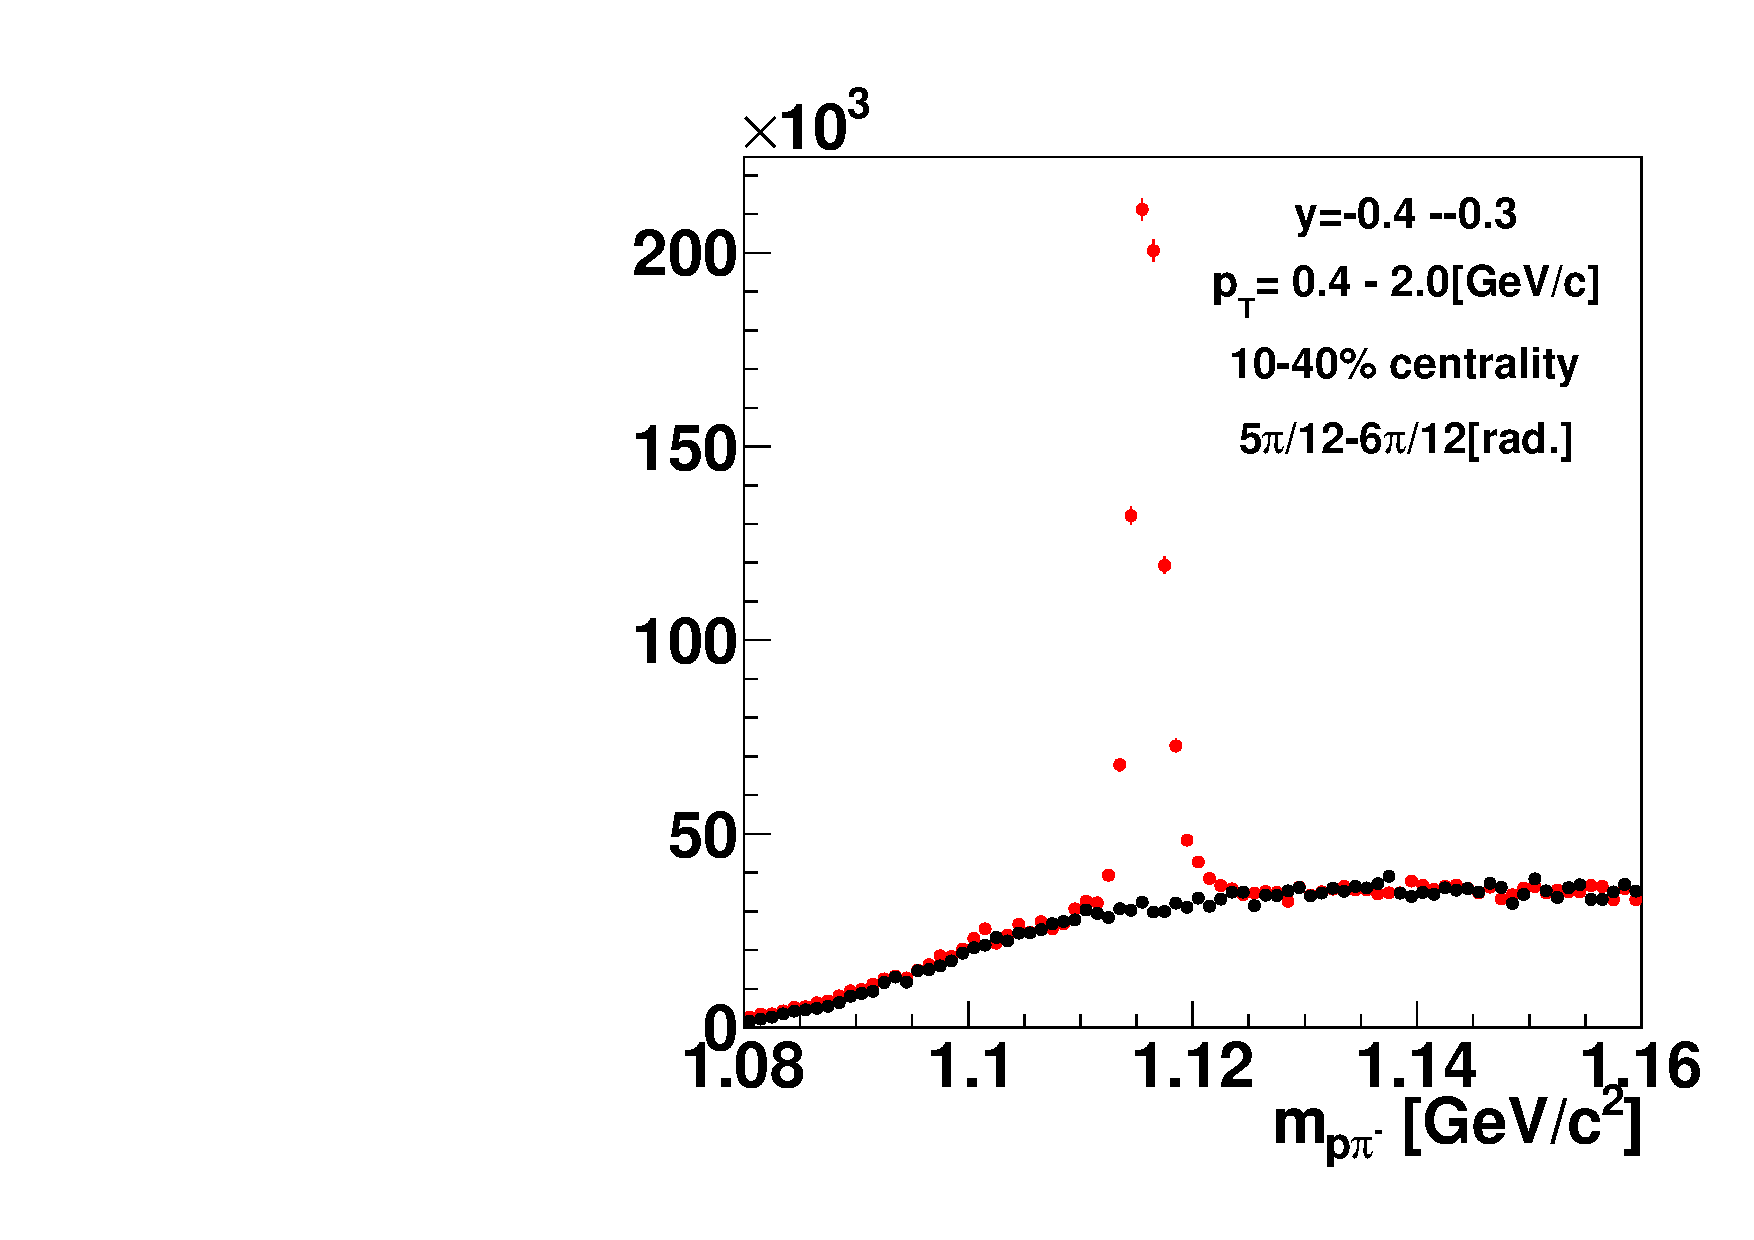
\includegraphics[width=0.14\linewidth]{chapterX/fig/ld_v1_sig/kf_ptslice0_cent1_ld_flow_phi6_rap8_check.pdf}
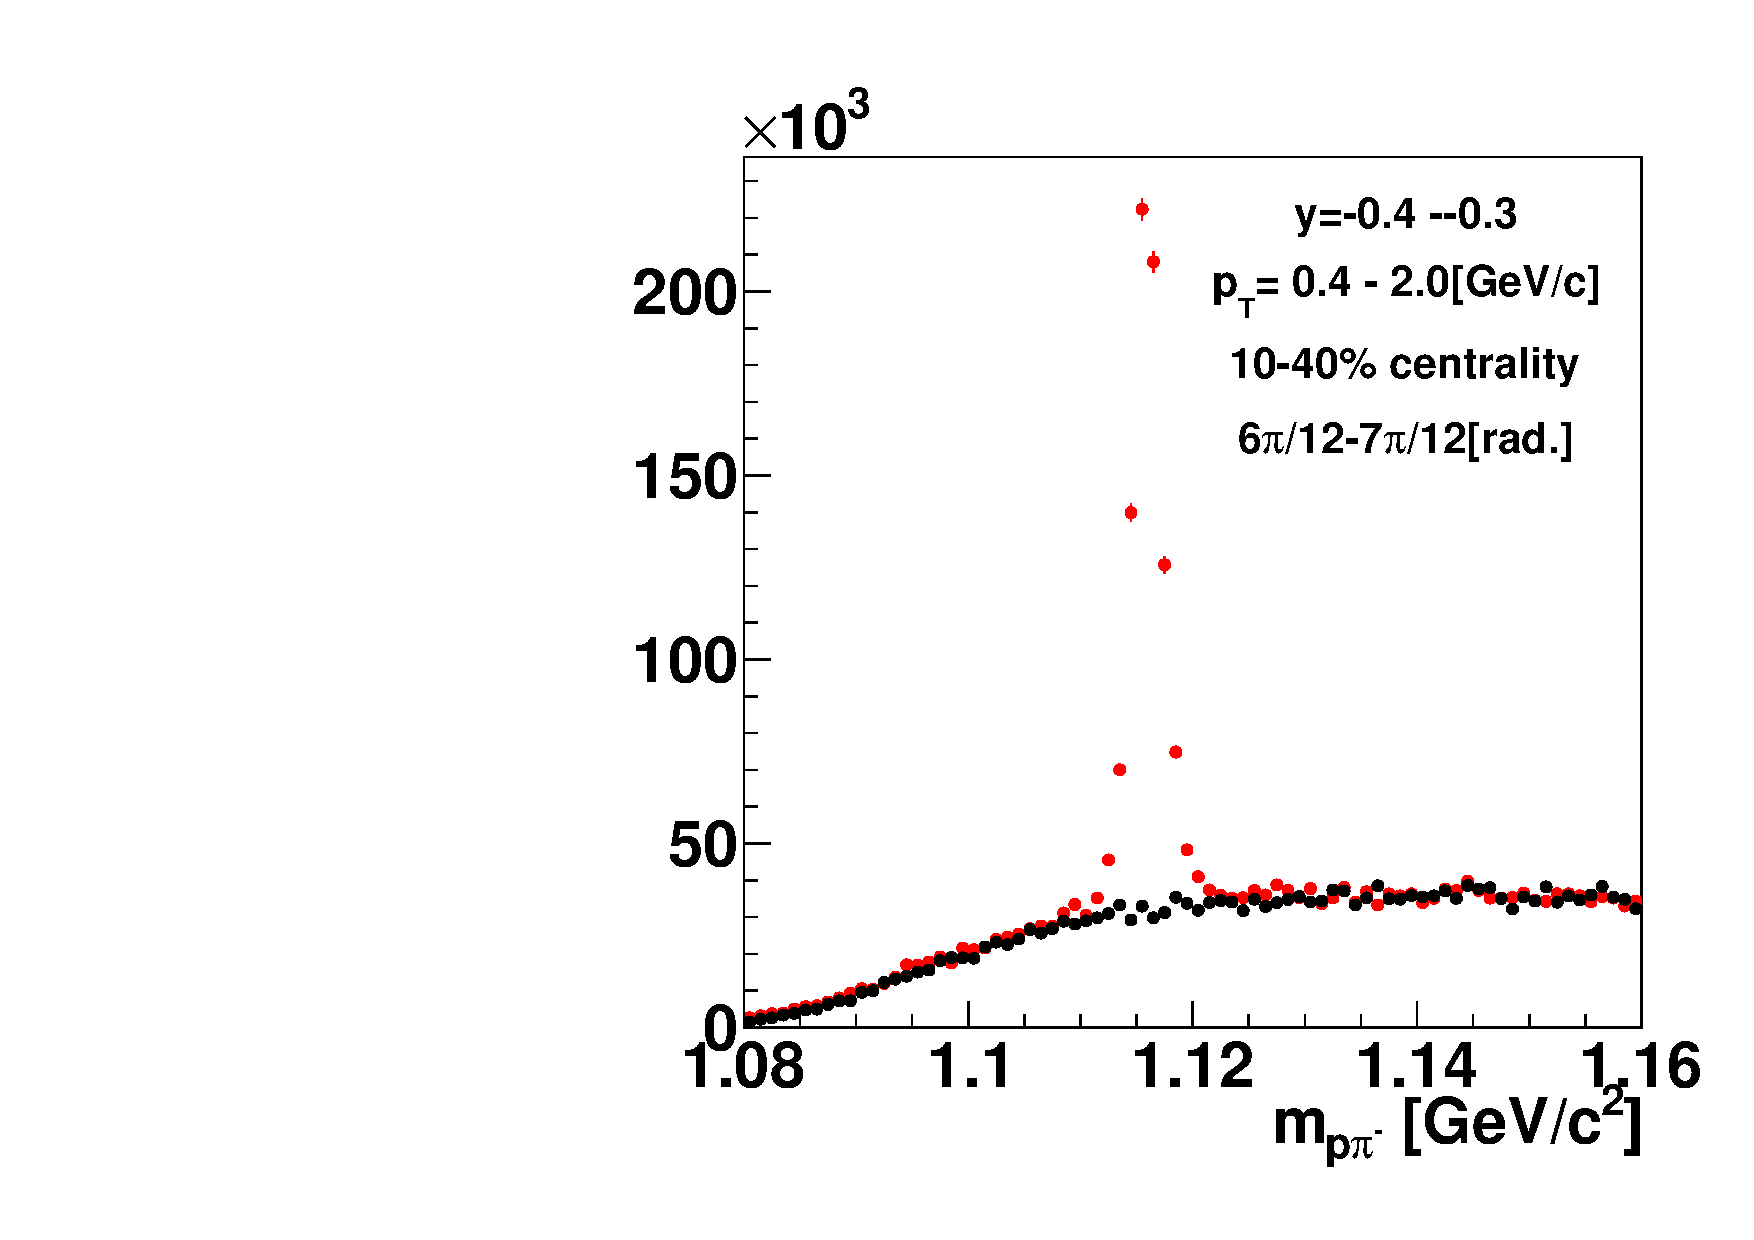
\includegraphics[width=0.14\linewidth]{chapterX/fig/ld_v1_sig/kf_ptslice0_cent1_ld_flow_phi7_rap8_check.pdf}
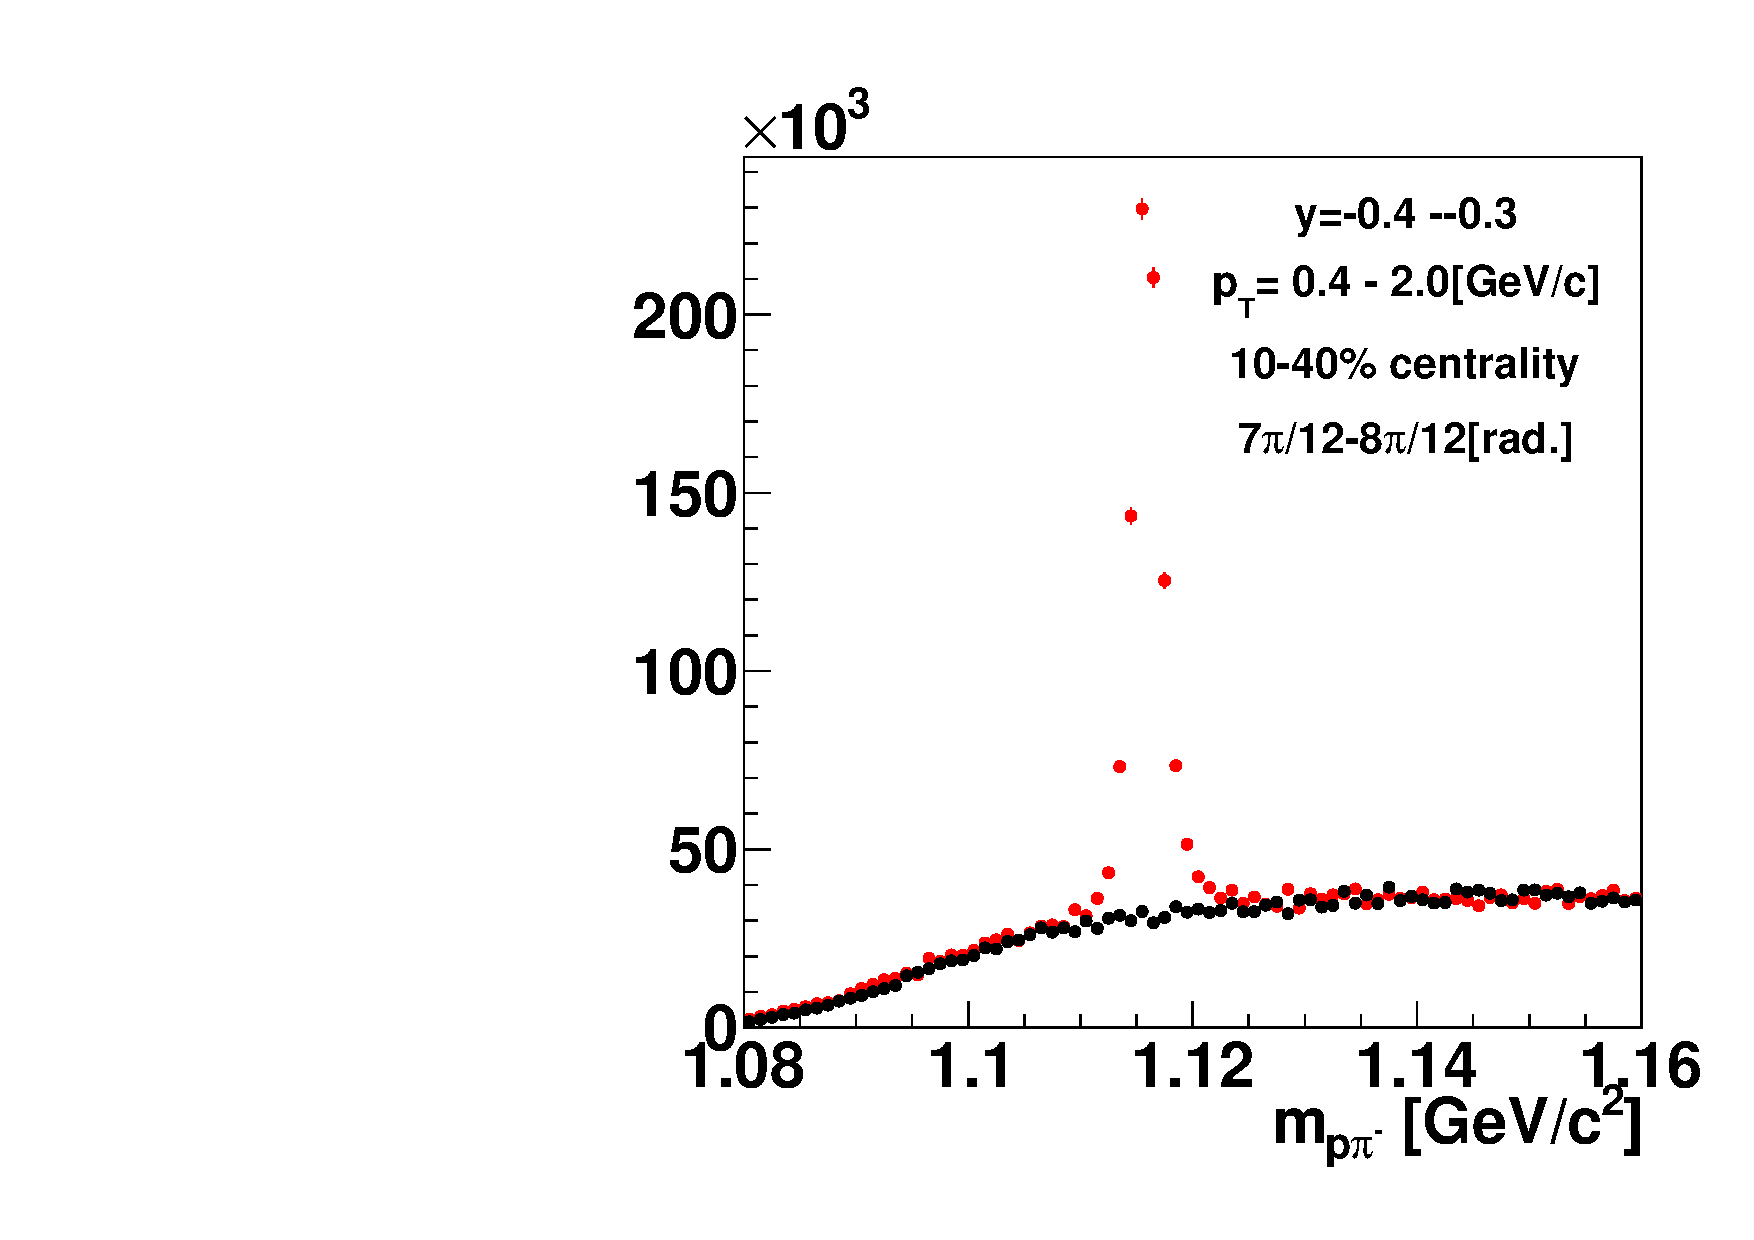
\includegraphics[width=0.14\linewidth]{chapterX/fig/ld_v1_sig/kf_ptslice0_cent1_ld_flow_phi8_rap8_check.pdf}
\includegraphics[width=0.14\linewidth]{chapterX/fig/ld_v1_sig/kf_ptslice0_cent1_ld_flow_phi9_rap8_check.pdf}
\includegraphics[width=0.14\linewidth]{chapterX/fig/ld_v1_sig/kf_ptslice0_cent1_ld_flow_phi10_rap8_check.pdf}
\includegraphics[width=0.14\linewidth]{chapterX/fig/ld_v1_sig/kf_ptslice0_cent1_ld_flow_phi11_rap8_check.pdf}
\includegraphics[width=0.14\linewidth]{chapterX/fig/ld_v1_sig/kf_ptslice0_cent1_ld_flow_phi12_rap8_check.pdf}

\includegraphics[width=0.14\linewidth]{chapterX/fig/ld_v1_sig/kf_ptslice0_cent1_ld_flow_phi1_rap9_check.pdf}
\includegraphics[width=0.14\linewidth]{chapterX/fig/ld_v1_sig/kf_ptslice0_cent1_ld_flow_phi2_rap9_check.pdf}
\includegraphics[width=0.14\linewidth]{chapterX/fig/ld_v1_sig/kf_ptslice0_cent1_ld_flow_phi3_rap9_check.pdf}
\includegraphics[width=0.14\linewidth]{chapterX/fig/ld_v1_sig/kf_ptslice0_cent1_ld_flow_phi4_rap9_check.pdf}
\includegraphics[width=0.14\linewidth]{chapterX/fig/ld_v1_sig/kf_ptslice0_cent1_ld_flow_phi5_rap9_check.pdf}
\includegraphics[width=0.14\linewidth]{chapterX/fig/ld_v1_sig/kf_ptslice0_cent1_ld_flow_phi6_rap9_check.pdf}
\includegraphics[width=0.14\linewidth]{chapterX/fig/ld_v1_sig/kf_ptslice0_cent1_ld_flow_phi7_rap9_check.pdf}
\includegraphics[width=0.14\linewidth]{chapterX/fig/ld_v1_sig/kf_ptslice0_cent1_ld_flow_phi8_rap9_check.pdf}
\includegraphics[width=0.14\linewidth]{chapterX/fig/ld_v1_sig/kf_ptslice0_cent1_ld_flow_phi9_rap9_check.pdf}
\includegraphics[width=0.14\linewidth]{chapterX/fig/ld_v1_sig/kf_ptslice0_cent1_ld_flow_phi10_rap9_check.pdf}
\includegraphics[width=0.14\linewidth]{chapterX/fig/ld_v1_sig/kf_ptslice0_cent1_ld_flow_phi11_rap9_check.pdf}
\includegraphics[width=0.14\linewidth]{chapterX/fig/ld_v1_sig/kf_ptslice0_cent1_ld_flow_phi12_rap9_check.pdf}

\caption{Signal and background invariant mass distribution for $p-\pi$ pairs in different rapidity and phi bins, for $10-40\%$.}
\label{ld_v1_sig_raw}
\end{figure}

\begin{figure}[h]
\includegraphics[width=0.14\linewidth]{chapterX/fig/ld_v1_sig/kf_ptslice0_cent1_ld_flow_phi1_rap10_check.pdf}
\includegraphics[width=0.14\linewidth]{chapterX/fig/ld_v1_sig/kf_ptslice0_cent1_ld_flow_phi2_rap10_check.pdf}
\includegraphics[width=0.14\linewidth]{chapterX/fig/ld_v1_sig/kf_ptslice0_cent1_ld_flow_phi3_rap10_check.pdf}
\includegraphics[width=0.14\linewidth]{chapterX/fig/ld_v1_sig/kf_ptslice0_cent1_ld_flow_phi4_rap10_check.pdf}
\includegraphics[width=0.14\linewidth]{chapterX/fig/ld_v1_sig/kf_ptslice0_cent1_ld_flow_phi5_rap10_check.pdf}
\includegraphics[width=0.14\linewidth]{chapterX/fig/ld_v1_sig/kf_ptslice0_cent1_ld_flow_phi6_rap10_check.pdf}
\includegraphics[width=0.14\linewidth]{chapterX/fig/ld_v1_sig/kf_ptslice0_cent1_ld_flow_phi7_rap10_check.pdf}
\includegraphics[width=0.14\linewidth]{chapterX/fig/ld_v1_sig/kf_ptslice0_cent1_ld_flow_phi8_rap10_check.pdf}
\includegraphics[width=0.14\linewidth]{chapterX/fig/ld_v1_sig/kf_ptslice0_cent1_ld_flow_phi9_rap10_check.pdf}
\includegraphics[width=0.14\linewidth]{chapterX/fig/ld_v1_sig/kf_ptslice0_cent1_ld_flow_phi10_rap10_check.pdf}
\includegraphics[width=0.14\linewidth]{chapterX/fig/ld_v1_sig/kf_ptslice0_cent1_ld_flow_phi11_rap10_check.pdf}
\includegraphics[width=0.14\linewidth]{chapterX/fig/ld_v1_sig/kf_ptslice0_cent1_ld_flow_phi12_rap10_check.pdf}

\includegraphics[width=0.14\linewidth]{chapterX/fig/ld_v1_sig/kf_ptslice0_cent1_ld_flow_phi1_rap11_check.pdf}
\includegraphics[width=0.14\linewidth]{chapterX/fig/ld_v1_sig/kf_ptslice0_cent1_ld_flow_phi2_rap11_check.pdf}
\includegraphics[width=0.14\linewidth]{chapterX/fig/ld_v1_sig/kf_ptslice0_cent1_ld_flow_phi3_rap11_check.pdf}
\includegraphics[width=0.14\linewidth]{chapterX/fig/ld_v1_sig/kf_ptslice0_cent1_ld_flow_phi4_rap11_check.pdf}
\includegraphics[width=0.14\linewidth]{chapterX/fig/ld_v1_sig/kf_ptslice0_cent1_ld_flow_phi5_rap11_check.pdf}
\includegraphics[width=0.14\linewidth]{chapterX/fig/ld_v1_sig/kf_ptslice0_cent1_ld_flow_phi6_rap11_check.pdf}
\includegraphics[width=0.14\linewidth]{chapterX/fig/ld_v1_sig/kf_ptslice0_cent1_ld_flow_phi7_rap11_check.pdf}
\includegraphics[width=0.14\linewidth]{chapterX/fig/ld_v1_sig/kf_ptslice0_cent1_ld_flow_phi8_rap11_check.pdf}
\includegraphics[width=0.14\linewidth]{chapterX/fig/ld_v1_sig/kf_ptslice0_cent1_ld_flow_phi9_rap11_check.pdf}
\includegraphics[width=0.14\linewidth]{chapterX/fig/ld_v1_sig/kf_ptslice0_cent1_ld_flow_phi10_rap11_check.pdf}
\includegraphics[width=0.14\linewidth]{chapterX/fig/ld_v1_sig/kf_ptslice0_cent1_ld_flow_phi11_rap11_check.pdf}
\includegraphics[width=0.14\linewidth]{chapterX/fig/ld_v1_sig/kf_ptslice0_cent1_ld_flow_phi12_rap11_check.pdf}

\includegraphics[width=0.14\linewidth]{chapterX/fig/ld_v1_sig/kf_ptslice0_cent1_ld_flow_phi1_rap12_check.pdf}
\includegraphics[width=0.14\linewidth]{chapterX/fig/ld_v1_sig/kf_ptslice0_cent1_ld_flow_phi2_rap12_check.pdf}
\includegraphics[width=0.14\linewidth]{chapterX/fig/ld_v1_sig/kf_ptslice0_cent1_ld_flow_phi3_rap12_check.pdf}
\includegraphics[width=0.14\linewidth]{chapterX/fig/ld_v1_sig/kf_ptslice0_cent1_ld_flow_phi4_rap12_check.pdf}
\includegraphics[width=0.14\linewidth]{chapterX/fig/ld_v1_sig/kf_ptslice0_cent1_ld_flow_phi5_rap12_check.pdf}
\includegraphics[width=0.14\linewidth]{chapterX/fig/ld_v1_sig/kf_ptslice0_cent1_ld_flow_phi6_rap12_check.pdf}
\includegraphics[width=0.14\linewidth]{chapterX/fig/ld_v1_sig/kf_ptslice0_cent1_ld_flow_phi7_rap12_check.pdf}
\includegraphics[width=0.14\linewidth]{chapterX/fig/ld_v1_sig/kf_ptslice0_cent1_ld_flow_phi8_rap12_check.pdf}
\includegraphics[width=0.14\linewidth]{chapterX/fig/ld_v1_sig/kf_ptslice0_cent1_ld_flow_phi9_rap12_check.pdf}
\includegraphics[width=0.14\linewidth]{chapterX/fig/ld_v1_sig/kf_ptslice0_cent1_ld_flow_phi10_rap12_check.pdf}
\includegraphics[width=0.14\linewidth]{chapterX/fig/ld_v1_sig/kf_ptslice0_cent1_ld_flow_phi11_rap12_check.pdf}
\includegraphics[width=0.14\linewidth]{chapterX/fig/ld_v1_sig/kf_ptslice0_cent1_ld_flow_phi12_rap12_check.pdf}

\includegraphics[width=0.14\linewidth]{chapterX/fig/ld_v1_sig/kf_ptslice0_cent1_ld_flow_phi1_rap13_check.pdf}
\includegraphics[width=0.14\linewidth]{chapterX/fig/ld_v1_sig/kf_ptslice0_cent1_ld_flow_phi2_rap13_check.pdf}
\includegraphics[width=0.14\linewidth]{chapterX/fig/ld_v1_sig/kf_ptslice0_cent1_ld_flow_phi3_rap13_check.pdf}
\includegraphics[width=0.14\linewidth]{chapterX/fig/ld_v1_sig/kf_ptslice0_cent1_ld_flow_phi4_rap13_check.pdf}
\includegraphics[width=0.14\linewidth]{chapterX/fig/ld_v1_sig/kf_ptslice0_cent1_ld_flow_phi5_rap13_check.pdf}
\includegraphics[width=0.14\linewidth]{chapterX/fig/ld_v1_sig/kf_ptslice0_cent1_ld_flow_phi6_rap13_check.pdf}
\includegraphics[width=0.14\linewidth]{chapterX/fig/ld_v1_sig/kf_ptslice0_cent1_ld_flow_phi7_rap13_check.pdf}
\includegraphics[width=0.14\linewidth]{chapterX/fig/ld_v1_sig/kf_ptslice0_cent1_ld_flow_phi8_rap13_check.pdf}
\includegraphics[width=0.14\linewidth]{chapterX/fig/ld_v1_sig/kf_ptslice0_cent1_ld_flow_phi9_rap13_check.pdf}
\includegraphics[width=0.14\linewidth]{chapterX/fig/ld_v1_sig/kf_ptslice0_cent1_ld_flow_phi10_rap13_check.pdf}
\includegraphics[width=0.14\linewidth]{chapterX/fig/ld_v1_sig/kf_ptslice0_cent1_ld_flow_phi11_rap13_check.pdf}
\includegraphics[width=0.14\linewidth]{chapterX/fig/ld_v1_sig/kf_ptslice0_cent1_ld_flow_phi12_rap13_check.pdf}

\includegraphics[width=0.14\linewidth]{chapterX/fig/ld_v1_sig/kf_ptslice0_cent1_ld_flow_phi1_rap14_check.pdf}
\includegraphics[width=0.14\linewidth]{chapterX/fig/ld_v1_sig/kf_ptslice0_cent1_ld_flow_phi2_rap14_check.pdf}
\includegraphics[width=0.14\linewidth]{chapterX/fig/ld_v1_sig/kf_ptslice0_cent1_ld_flow_phi3_rap14_check.pdf}
\includegraphics[width=0.14\linewidth]{chapterX/fig/ld_v1_sig/kf_ptslice0_cent1_ld_flow_phi4_rap14_check.pdf}
\includegraphics[width=0.14\linewidth]{chapterX/fig/ld_v1_sig/kf_ptslice0_cent1_ld_flow_phi5_rap14_check.pdf}
\includegraphics[width=0.14\linewidth]{chapterX/fig/ld_v1_sig/kf_ptslice0_cent1_ld_flow_phi6_rap14_check.pdf}
\includegraphics[width=0.14\linewidth]{chapterX/fig/ld_v1_sig/kf_ptslice0_cent1_ld_flow_phi7_rap14_check.pdf}
\includegraphics[width=0.14\linewidth]{chapterX/fig/ld_v1_sig/kf_ptslice0_cent1_ld_flow_phi8_rap14_check.pdf}
\includegraphics[width=0.14\linewidth]{chapterX/fig/ld_v1_sig/kf_ptslice0_cent1_ld_flow_phi9_rap14_check.pdf}
\includegraphics[width=0.14\linewidth]{chapterX/fig/ld_v1_sig/kf_ptslice0_cent1_ld_flow_phi10_rap14_check.pdf}
\includegraphics[width=0.14\linewidth]{chapterX/fig/ld_v1_sig/kf_ptslice0_cent1_ld_flow_phi11_rap14_check.pdf}
\includegraphics[width=0.14\linewidth]{chapterX/fig/ld_v1_sig/kf_ptslice0_cent1_ld_flow_phi12_rap14_check.pdf}

\caption{Signal and background invariant mass distribution for $p-\pi$ pairs in different rapidity and phi bins, for $10-40\%$.}
\label{ld_v1_sig_raw2}
\end{figure}


\begin{figure}[h]
\includegraphics[width=0.14\linewidth]{chapterX/fig/ld_v1_sig/kf_ptslice0_cent1_ld_flow_phi1_rap5.pdf}
\includegraphics[width=0.14\linewidth]{chapterX/fig/ld_v1_sig/kf_ptslice0_cent1_ld_flow_phi2_rap5.pdf}
\includegraphics[width=0.14\linewidth]{chapterX/fig/ld_v1_sig/kf_ptslice0_cent1_ld_flow_phi3_rap5.pdf}
\includegraphics[width=0.14\linewidth]{chapterX/fig/ld_v1_sig/kf_ptslice0_cent1_ld_flow_phi4_rap5.pdf}
\includegraphics[width=0.14\linewidth]{chapterX/fig/ld_v1_sig/kf_ptslice0_cent1_ld_flow_phi5_rap5.pdf}
\includegraphics[width=0.14\linewidth]{chapterX/fig/ld_v1_sig/kf_ptslice0_cent1_ld_flow_phi6_rap5.pdf}
\includegraphics[width=0.14\linewidth]{chapterX/fig/ld_v1_sig/kf_ptslice0_cent1_ld_flow_phi7_rap5.pdf}
\includegraphics[width=0.14\linewidth]{chapterX/fig/ld_v1_sig/kf_ptslice0_cent1_ld_flow_phi8_rap5.pdf}
\includegraphics[width=0.14\linewidth]{chapterX/fig/ld_v1_sig/kf_ptslice0_cent1_ld_flow_phi9_rap5.pdf}
\includegraphics[width=0.14\linewidth]{chapterX/fig/ld_v1_sig/kf_ptslice0_cent1_ld_flow_phi10_rap5.pdf}
\includegraphics[width=0.14\linewidth]{chapterX/fig/ld_v1_sig/kf_ptslice0_cent1_ld_flow_phi11_rap5.pdf}
\includegraphics[width=0.14\linewidth]{chapterX/fig/ld_v1_sig/kf_ptslice0_cent1_ld_flow_phi12_rap5.pdf}

\includegraphics[width=0.14\linewidth]{chapterX/fig/ld_v1_sig/kf_ptslice0_cent1_ld_flow_phi1_rap6.pdf}
\includegraphics[width=0.14\linewidth]{chapterX/fig/ld_v1_sig/kf_ptslice0_cent1_ld_flow_phi2_rap6.pdf}
\includegraphics[width=0.14\linewidth]{chapterX/fig/ld_v1_sig/kf_ptslice0_cent1_ld_flow_phi3_rap6.pdf}
\includegraphics[width=0.14\linewidth]{chapterX/fig/ld_v1_sig/kf_ptslice0_cent1_ld_flow_phi4_rap6.pdf}
\includegraphics[width=0.14\linewidth]{chapterX/fig/ld_v1_sig/kf_ptslice0_cent1_ld_flow_phi5_rap6.pdf}
\includegraphics[width=0.14\linewidth]{chapterX/fig/ld_v1_sig/kf_ptslice0_cent1_ld_flow_phi6_rap6.pdf}
\includegraphics[width=0.14\linewidth]{chapterX/fig/ld_v1_sig/kf_ptslice0_cent1_ld_flow_phi7_rap6.pdf}
\includegraphics[width=0.14\linewidth]{chapterX/fig/ld_v1_sig/kf_ptslice0_cent1_ld_flow_phi8_rap6.pdf}
\includegraphics[width=0.14\linewidth]{chapterX/fig/ld_v1_sig/kf_ptslice0_cent1_ld_flow_phi9_rap6.pdf}
\includegraphics[width=0.14\linewidth]{chapterX/fig/ld_v1_sig/kf_ptslice0_cent1_ld_flow_phi10_rap6.pdf}
\includegraphics[width=0.14\linewidth]{chapterX/fig/ld_v1_sig/kf_ptslice0_cent1_ld_flow_phi11_rap6.pdf}
\includegraphics[width=0.14\linewidth]{chapterX/fig/ld_v1_sig/kf_ptslice0_cent1_ld_flow_phi12_rap6.pdf}

\includegraphics[width=0.14\linewidth]{chapterX/fig/ld_v1_sig/kf_ptslice0_cent1_ld_flow_phi1_rap7.pdf}
\includegraphics[width=0.14\linewidth]{chapterX/fig/ld_v1_sig/kf_ptslice0_cent1_ld_flow_phi2_rap7.pdf}
\includegraphics[width=0.14\linewidth]{chapterX/fig/ld_v1_sig/kf_ptslice0_cent1_ld_flow_phi3_rap7.pdf}
\includegraphics[width=0.14\linewidth]{chapterX/fig/ld_v1_sig/kf_ptslice0_cent1_ld_flow_phi4_rap7.pdf}
\includegraphics[width=0.14\linewidth]{chapterX/fig/ld_v1_sig/kf_ptslice0_cent1_ld_flow_phi5_rap7.pdf}
\includegraphics[width=0.14\linewidth]{chapterX/fig/ld_v1_sig/kf_ptslice0_cent1_ld_flow_phi6_rap7.pdf}
\includegraphics[width=0.14\linewidth]{chapterX/fig/ld_v1_sig/kf_ptslice0_cent1_ld_flow_phi7_rap7.pdf}
\includegraphics[width=0.14\linewidth]{chapterX/fig/ld_v1_sig/kf_ptslice0_cent1_ld_flow_phi8_rap7.pdf}
\includegraphics[width=0.14\linewidth]{chapterX/fig/ld_v1_sig/kf_ptslice0_cent1_ld_flow_phi9_rap7.pdf}
\includegraphics[width=0.14\linewidth]{chapterX/fig/ld_v1_sig/kf_ptslice0_cent1_ld_flow_phi10_rap7.pdf}
\includegraphics[width=0.14\linewidth]{chapterX/fig/ld_v1_sig/kf_ptslice0_cent1_ld_flow_phi11_rap7.pdf}
\includegraphics[width=0.14\linewidth]{chapterX/fig/ld_v1_sig/kf_ptslice0_cent1_ld_flow_phi12_rap7.pdf}

\includegraphics[width=0.14\linewidth]{chapterX/fig/ld_v1_sig/kf_ptslice0_cent1_ld_flow_phi1_rap8.pdf}
\includegraphics[width=0.14\linewidth]{chapterX/fig/ld_v1_sig/kf_ptslice0_cent1_ld_flow_phi2_rap8.pdf}
\includegraphics[width=0.14\linewidth]{chapterX/fig/ld_v1_sig/kf_ptslice0_cent1_ld_flow_phi3_rap8.pdf}
\includegraphics[width=0.14\linewidth]{chapterX/fig/ld_v1_sig/kf_ptslice0_cent1_ld_flow_phi4_rap8.pdf}
\includegraphics[width=0.14\linewidth]{chapterX/fig/ld_v1_sig/kf_ptslice0_cent1_ld_flow_phi5_rap8.pdf}
\includegraphics[width=0.14\linewidth]{chapterX/fig/ld_v1_sig/kf_ptslice0_cent1_ld_flow_phi6_rap8.pdf}
\includegraphics[width=0.14\linewidth]{chapterX/fig/ld_v1_sig/kf_ptslice0_cent1_ld_flow_phi7_rap8.pdf}
\includegraphics[width=0.14\linewidth]{chapterX/fig/ld_v1_sig/kf_ptslice0_cent1_ld_flow_phi8_rap8.pdf}
\includegraphics[width=0.14\linewidth]{chapterX/fig/ld_v1_sig/kf_ptslice0_cent1_ld_flow_phi9_rap8.pdf}
\includegraphics[width=0.14\linewidth]{chapterX/fig/ld_v1_sig/kf_ptslice0_cent1_ld_flow_phi10_rap8.pdf}
\includegraphics[width=0.14\linewidth]{chapterX/fig/ld_v1_sig/kf_ptslice0_cent1_ld_flow_phi11_rap8.pdf}
\includegraphics[width=0.14\linewidth]{chapterX/fig/ld_v1_sig/kf_ptslice0_cent1_ld_flow_phi12_rap8.pdf}

\includegraphics[width=0.14\linewidth]{chapterX/fig/ld_v1_sig/kf_ptslice0_cent1_ld_flow_phi1_rap9.pdf}
\includegraphics[width=0.14\linewidth]{chapterX/fig/ld_v1_sig/kf_ptslice0_cent1_ld_flow_phi2_rap9.pdf}
\includegraphics[width=0.14\linewidth]{chapterX/fig/ld_v1_sig/kf_ptslice0_cent1_ld_flow_phi3_rap9.pdf}
\includegraphics[width=0.14\linewidth]{chapterX/fig/ld_v1_sig/kf_ptslice0_cent1_ld_flow_phi4_rap9.pdf}
\includegraphics[width=0.14\linewidth]{chapterX/fig/ld_v1_sig/kf_ptslice0_cent1_ld_flow_phi5_rap9.pdf}
\includegraphics[width=0.14\linewidth]{chapterX/fig/ld_v1_sig/kf_ptslice0_cent1_ld_flow_phi6_rap9.pdf}
\includegraphics[width=0.14\linewidth]{chapterX/fig/ld_v1_sig/kf_ptslice0_cent1_ld_flow_phi7_rap9.pdf}
\includegraphics[width=0.14\linewidth]{chapterX/fig/ld_v1_sig/kf_ptslice0_cent1_ld_flow_phi8_rap9.pdf}
\includegraphics[width=0.14\linewidth]{chapterX/fig/ld_v1_sig/kf_ptslice0_cent1_ld_flow_phi9_rap9.pdf}
\includegraphics[width=0.14\linewidth]{chapterX/fig/ld_v1_sig/kf_ptslice0_cent1_ld_flow_phi10_rap9.pdf}
\includegraphics[width=0.14\linewidth]{chapterX/fig/ld_v1_sig/kf_ptslice0_cent1_ld_flow_phi11_rap9.pdf}
\includegraphics[width=0.14\linewidth]{chapterX/fig/ld_v1_sig/kf_ptslice0_cent1_ld_flow_phi12_rap9.pdf}

\caption{Subtracted data invariant mass distribution for $p-\pi$ pairs in different rapidity and phi bins, for $10-40\%$.}
\label{ld_v1_sig}
\end{figure}

\begin{figure}[h]
\includegraphics[width=0.14\linewidth]{chapterX/fig/ld_v1_sig/kf_ptslice0_cent1_ld_flow_phi1_rap10.pdf}
\includegraphics[width=0.14\linewidth]{chapterX/fig/ld_v1_sig/kf_ptslice0_cent1_ld_flow_phi2_rap10.pdf}
\includegraphics[width=0.14\linewidth]{chapterX/fig/ld_v1_sig/kf_ptslice0_cent1_ld_flow_phi3_rap10.pdf}
\includegraphics[width=0.14\linewidth]{chapterX/fig/ld_v1_sig/kf_ptslice0_cent1_ld_flow_phi4_rap10.pdf}
\includegraphics[width=0.14\linewidth]{chapterX/fig/ld_v1_sig/kf_ptslice0_cent1_ld_flow_phi5_rap10.pdf}
\includegraphics[width=0.14\linewidth]{chapterX/fig/ld_v1_sig/kf_ptslice0_cent1_ld_flow_phi6_rap10.pdf}
\includegraphics[width=0.14\linewidth]{chapterX/fig/ld_v1_sig/kf_ptslice0_cent1_ld_flow_phi7_rap10.pdf}
\includegraphics[width=0.14\linewidth]{chapterX/fig/ld_v1_sig/kf_ptslice0_cent1_ld_flow_phi8_rap10.pdf}
\includegraphics[width=0.14\linewidth]{chapterX/fig/ld_v1_sig/kf_ptslice0_cent1_ld_flow_phi9_rap10.pdf}
\includegraphics[width=0.14\linewidth]{chapterX/fig/ld_v1_sig/kf_ptslice0_cent1_ld_flow_phi10_rap10.pdf}
\includegraphics[width=0.14\linewidth]{chapterX/fig/ld_v1_sig/kf_ptslice0_cent1_ld_flow_phi11_rap10.pdf}
\includegraphics[width=0.14\linewidth]{chapterX/fig/ld_v1_sig/kf_ptslice0_cent1_ld_flow_phi12_rap10.pdf}

\includegraphics[width=0.14\linewidth]{chapterX/fig/ld_v1_sig/kf_ptslice0_cent1_ld_flow_phi1_rap11.pdf}
\includegraphics[width=0.14\linewidth]{chapterX/fig/ld_v1_sig/kf_ptslice0_cent1_ld_flow_phi2_rap11.pdf}
\includegraphics[width=0.14\linewidth]{chapterX/fig/ld_v1_sig/kf_ptslice0_cent1_ld_flow_phi3_rap11.pdf}
\includegraphics[width=0.14\linewidth]{chapterX/fig/ld_v1_sig/kf_ptslice0_cent1_ld_flow_phi4_rap11.pdf}
\includegraphics[width=0.14\linewidth]{chapterX/fig/ld_v1_sig/kf_ptslice0_cent1_ld_flow_phi5_rap11.pdf}
\includegraphics[width=0.14\linewidth]{chapterX/fig/ld_v1_sig/kf_ptslice0_cent1_ld_flow_phi6_rap11.pdf}
\includegraphics[width=0.14\linewidth]{chapterX/fig/ld_v1_sig/kf_ptslice0_cent1_ld_flow_phi7_rap11.pdf}
\includegraphics[width=0.14\linewidth]{chapterX/fig/ld_v1_sig/kf_ptslice0_cent1_ld_flow_phi8_rap11.pdf}
\includegraphics[width=0.14\linewidth]{chapterX/fig/ld_v1_sig/kf_ptslice0_cent1_ld_flow_phi9_rap11.pdf}
\includegraphics[width=0.14\linewidth]{chapterX/fig/ld_v1_sig/kf_ptslice0_cent1_ld_flow_phi10_rap11.pdf}
\includegraphics[width=0.14\linewidth]{chapterX/fig/ld_v1_sig/kf_ptslice0_cent1_ld_flow_phi11_rap11.pdf}
\includegraphics[width=0.14\linewidth]{chapterX/fig/ld_v1_sig/kf_ptslice0_cent1_ld_flow_phi12_rap11.pdf}

\includegraphics[width=0.14\linewidth]{chapterX/fig/ld_v1_sig/kf_ptslice0_cent1_ld_flow_phi1_rap12.pdf}
\includegraphics[width=0.14\linewidth]{chapterX/fig/ld_v1_sig/kf_ptslice0_cent1_ld_flow_phi2_rap12.pdf}
\includegraphics[width=0.14\linewidth]{chapterX/fig/ld_v1_sig/kf_ptslice0_cent1_ld_flow_phi3_rap12.pdf}
\includegraphics[width=0.14\linewidth]{chapterX/fig/ld_v1_sig/kf_ptslice0_cent1_ld_flow_phi4_rap12.pdf}
\includegraphics[width=0.14\linewidth]{chapterX/fig/ld_v1_sig/kf_ptslice0_cent1_ld_flow_phi5_rap12.pdf}
\includegraphics[width=0.14\linewidth]{chapterX/fig/ld_v1_sig/kf_ptslice0_cent1_ld_flow_phi6_rap12.pdf}
\includegraphics[width=0.14\linewidth]{chapterX/fig/ld_v1_sig/kf_ptslice0_cent1_ld_flow_phi7_rap12.pdf}
\includegraphics[width=0.14\linewidth]{chapterX/fig/ld_v1_sig/kf_ptslice0_cent1_ld_flow_phi8_rap12.pdf}
\includegraphics[width=0.14\linewidth]{chapterX/fig/ld_v1_sig/kf_ptslice0_cent1_ld_flow_phi9_rap12.pdf}
\includegraphics[width=0.14\linewidth]{chapterX/fig/ld_v1_sig/kf_ptslice0_cent1_ld_flow_phi10_rap12.pdf}
\includegraphics[width=0.14\linewidth]{chapterX/fig/ld_v1_sig/kf_ptslice0_cent1_ld_flow_phi11_rap12.pdf}
\includegraphics[width=0.14\linewidth]{chapterX/fig/ld_v1_sig/kf_ptslice0_cent1_ld_flow_phi12_rap12.pdf}

\includegraphics[width=0.14\linewidth]{chapterX/fig/ld_v1_sig/kf_ptslice0_cent1_ld_flow_phi1_rap13.pdf}
\includegraphics[width=0.14\linewidth]{chapterX/fig/ld_v1_sig/kf_ptslice0_cent1_ld_flow_phi2_rap13.pdf}
\includegraphics[width=0.14\linewidth]{chapterX/fig/ld_v1_sig/kf_ptslice0_cent1_ld_flow_phi3_rap13.pdf}
\includegraphics[width=0.14\linewidth]{chapterX/fig/ld_v1_sig/kf_ptslice0_cent1_ld_flow_phi4_rap13.pdf}
\includegraphics[width=0.14\linewidth]{chapterX/fig/ld_v1_sig/kf_ptslice0_cent1_ld_flow_phi5_rap13.pdf}
\includegraphics[width=0.14\linewidth]{chapterX/fig/ld_v1_sig/kf_ptslice0_cent1_ld_flow_phi6_rap13.pdf}
\includegraphics[width=0.14\linewidth]{chapterX/fig/ld_v1_sig/kf_ptslice0_cent1_ld_flow_phi7_rap13.pdf}
\includegraphics[width=0.14\linewidth]{chapterX/fig/ld_v1_sig/kf_ptslice0_cent1_ld_flow_phi8_rap13.pdf}
\includegraphics[width=0.14\linewidth]{chapterX/fig/ld_v1_sig/kf_ptslice0_cent1_ld_flow_phi9_rap13.pdf}
\includegraphics[width=0.14\linewidth]{chapterX/fig/ld_v1_sig/kf_ptslice0_cent1_ld_flow_phi10_rap13.pdf}
\includegraphics[width=0.14\linewidth]{chapterX/fig/ld_v1_sig/kf_ptslice0_cent1_ld_flow_phi11_rap13.pdf}
\includegraphics[width=0.14\linewidth]{chapterX/fig/ld_v1_sig/kf_ptslice0_cent1_ld_flow_phi12_rap13.pdf}

\includegraphics[width=0.14\linewidth]{chapterX/fig/ld_v1_sig/kf_ptslice0_cent1_ld_flow_phi1_rap14.pdf}
\includegraphics[width=0.14\linewidth]{chapterX/fig/ld_v1_sig/kf_ptslice0_cent1_ld_flow_phi2_rap14.pdf}
\includegraphics[width=0.14\linewidth]{chapterX/fig/ld_v1_sig/kf_ptslice0_cent1_ld_flow_phi3_rap14.pdf}
\includegraphics[width=0.14\linewidth]{chapterX/fig/ld_v1_sig/kf_ptslice0_cent1_ld_flow_phi4_rap14.pdf}
\includegraphics[width=0.14\linewidth]{chapterX/fig/ld_v1_sig/kf_ptslice0_cent1_ld_flow_phi5_rap14.pdf}
\includegraphics[width=0.14\linewidth]{chapterX/fig/ld_v1_sig/kf_ptslice0_cent1_ld_flow_phi6_rap14.pdf}
\includegraphics[width=0.14\linewidth]{chapterX/fig/ld_v1_sig/kf_ptslice0_cent1_ld_flow_phi7_rap14.pdf}
\includegraphics[width=0.14\linewidth]{chapterX/fig/ld_v1_sig/kf_ptslice0_cent1_ld_flow_phi8_rap14.pdf}
\includegraphics[width=0.14\linewidth]{chapterX/fig/ld_v1_sig/kf_ptslice0_cent1_ld_flow_phi9_rap14.pdf}
\includegraphics[width=0.14\linewidth]{chapterX/fig/ld_v1_sig/kf_ptslice0_cent1_ld_flow_phi10_rap14.pdf}
\includegraphics[width=0.14\linewidth]{chapterX/fig/ld_v1_sig/kf_ptslice0_cent1_ld_flow_phi11_rap14.pdf}
\includegraphics[width=0.14\linewidth]{chapterX/fig/ld_v1_sig/kf_ptslice0_cent1_ld_flow_phi12_rap14.pdf}

\caption{Subtracted data invariant mass distribution for $p-\pi$ pairs in different rapidity and phi bins, for $10-40\%$.}
\label{ld_v1_sig2}
\end{figure}

After this procedure, we can obtain $dN/d(\phi-\Psi)$ as a function of $\phi-\Psi$. This is shown in Fig.~\ref{ldv1fit1040}, for each rapidity region, for centrality bin $10-40\%$. We then correct by the event plane resolution to obtain the corrected $v_{1}$. 

\begin{figure}[h]
\includegraphics[width=0.19\linewidth]{chapterX/fig/ld_v1_sig/ld_3gev_phi_cent1_pt0_rap5.pdf}
\includegraphics[width=0.19\linewidth]{chapterX/fig/ld_v1_sig/ld_3gev_phi_cent1_pt0_rap6.pdf}
\includegraphics[width=0.19\linewidth]{chapterX/fig/ld_v1_sig/ld_3gev_phi_cent1_pt0_rap7.pdf}
\includegraphics[width=0.19\linewidth]{chapterX/fig/ld_v1_sig/ld_3gev_phi_cent1_pt0_rap8.pdf}
\includegraphics[width=0.19\linewidth]{chapterX/fig/ld_v1_sig/ld_3gev_phi_cent1_pt0_rap9.pdf}
\includegraphics[width=0.19\linewidth]{chapterX/fig/ld_v1_sig/ld_3gev_phi_cent1_pt0_rap10.pdf}
\includegraphics[width=0.19\linewidth]{chapterX/fig/ld_v1_sig/ld_3gev_phi_cent1_pt0_rap11.pdf}
\includegraphics[width=0.19\linewidth]{chapterX/fig/ld_v1_sig/ld_3gev_phi_cent1_pt0_rap12.pdf}
\includegraphics[width=0.19\linewidth]{chapterX/fig/ld_v1_sig/ld_3gev_phi_cent1_pt0_rap13.pdf}
\includegraphics[width=0.19\linewidth]{chapterX/fig/ld_v1_sig/ld_3gev_phi_cent1_pt0_rap14.pdf}
\caption{$\Lambda$ signal count as a function of $\phi-\Psi$ in different rapidity bins, for $10-40\%$.}
\label{ldv1fit1040}
\end{figure}


We further plot $v_{1}$ as a function of $y$. As can be seen in Fig.~\ref{lddv1dyfit1040}, a small offset from $(0,0)$ was observed, similar to proton analysis. We fit with a third order function $y=a+bx+cx^{3}$ to obtain $dv_{1}/dy$ at $y=0$. The reflected data points are just for visualization purpose. 

\begin{figure}[h]
\includegraphics[width=0.5\linewidth]{chapterX/fig/ld_v1_sig/v1vy_centall_ptbin0.pdf}
\caption{$\Lambda$ $v_1$ as a function of $y$.}
\label{lddv1dyfit1040}
\end{figure}



\subsubsection{$v_2$ extraction for $\Lambda$}

The procedure is very similar to $v_1$ extraction. We extract $v_2$ for $10-40\%$, over the $p_{T}$ region $0.4-2.0$ [GeV/$c$], $y=-1 -0$. We divide into 4 rapidity bins of width 0.25. The projections of the histograms for $10-40\%$ are shown in Fig.~\ref{ld_v2_sig_raw}. To obtain the number of counts, we subtraction the background generated by rotation method, as shown in Fig.~\ref{ld_v2_sig}.

\begin{figure}[h]
\includegraphics[width=0.14\linewidth]{chapterX/fig/ld_v2_sig/kf_ptslice0_cent1_ld_flow_phi1_rap2_check.pdf}
\includegraphics[width=0.14\linewidth]{chapterX/fig/ld_v2_sig/kf_ptslice0_cent1_ld_flow_phi2_rap2_check.pdf}
\includegraphics[width=0.14\linewidth]{chapterX/fig/ld_v2_sig/kf_ptslice0_cent1_ld_flow_phi3_rap2_check.pdf}
\includegraphics[width=0.14\linewidth]{chapterX/fig/ld_v2_sig/kf_ptslice0_cent1_ld_flow_phi4_rap2_check.pdf}
\includegraphics[width=0.14\linewidth]{chapterX/fig/ld_v2_sig/kf_ptslice0_cent1_ld_flow_phi5_rap2_check.pdf}
\includegraphics[width=0.14\linewidth]{chapterX/fig/ld_v2_sig/kf_ptslice0_cent1_ld_flow_phi6_rap2_check.pdf}
\includegraphics[width=0.14\linewidth]{chapterX/fig/ld_v2_sig/kf_ptslice0_cent1_ld_flow_phi7_rap2_check.pdf}
\includegraphics[width=0.14\linewidth]{chapterX/fig/ld_v2_sig/kf_ptslice0_cent1_ld_flow_phi8_rap2_check.pdf}
\includegraphics[width=0.14\linewidth]{chapterX/fig/ld_v2_sig/kf_ptslice0_cent1_ld_flow_phi9_rap2_check.pdf}
\includegraphics[width=0.14\linewidth]{chapterX/fig/ld_v2_sig/kf_ptslice0_cent1_ld_flow_phi10_rap2_check.pdf}
\includegraphics[width=0.14\linewidth]{chapterX/fig/ld_v2_sig/kf_ptslice0_cent1_ld_flow_phi11_rap2_check.pdf}
\includegraphics[width=0.14\linewidth]{chapterX/fig/ld_v2_sig/kf_ptslice0_cent1_ld_flow_phi12_rap2_check.pdf}

\includegraphics[width=0.14\linewidth]{chapterX/fig/ld_v2_sig/kf_ptslice0_cent1_ld_flow_phi1_rap3_check.pdf}
\includegraphics[width=0.14\linewidth]{chapterX/fig/ld_v2_sig/kf_ptslice0_cent1_ld_flow_phi2_rap3_check.pdf}
\includegraphics[width=0.14\linewidth]{chapterX/fig/ld_v2_sig/kf_ptslice0_cent1_ld_flow_phi3_rap3_check.pdf}
\includegraphics[width=0.14\linewidth]{chapterX/fig/ld_v2_sig/kf_ptslice0_cent1_ld_flow_phi4_rap3_check.pdf}
\includegraphics[width=0.14\linewidth]{chapterX/fig/ld_v2_sig/kf_ptslice0_cent1_ld_flow_phi5_rap3_check.pdf}
\includegraphics[width=0.14\linewidth]{chapterX/fig/ld_v2_sig/kf_ptslice0_cent1_ld_flow_phi6_rap3_check.pdf}
\includegraphics[width=0.14\linewidth]{chapterX/fig/ld_v2_sig/kf_ptslice0_cent1_ld_flow_phi7_rap3_check.pdf}
\includegraphics[width=0.14\linewidth]{chapterX/fig/ld_v2_sig/kf_ptslice0_cent1_ld_flow_phi8_rap3_check.pdf}
\includegraphics[width=0.14\linewidth]{chapterX/fig/ld_v2_sig/kf_ptslice0_cent1_ld_flow_phi9_rap3_check.pdf}
\includegraphics[width=0.14\linewidth]{chapterX/fig/ld_v2_sig/kf_ptslice0_cent1_ld_flow_phi10_rap3_check.pdf}
\includegraphics[width=0.14\linewidth]{chapterX/fig/ld_v2_sig/kf_ptslice0_cent1_ld_flow_phi11_rap3_check.pdf}
\includegraphics[width=0.14\linewidth]{chapterX/fig/ld_v2_sig/kf_ptslice0_cent1_ld_flow_phi12_rap3_check.pdf}

\includegraphics[width=0.14\linewidth]{chapterX/fig/ld_v2_sig/kf_ptslice0_cent1_ld_flow_phi1_rap4_check.pdf}
\includegraphics[width=0.14\linewidth]{chapterX/fig/ld_v2_sig/kf_ptslice0_cent1_ld_flow_phi2_rap4_check.pdf}
\includegraphics[width=0.14\linewidth]{chapterX/fig/ld_v2_sig/kf_ptslice0_cent1_ld_flow_phi3_rap4_check.pdf}
\includegraphics[width=0.14\linewidth]{chapterX/fig/ld_v2_sig/kf_ptslice0_cent1_ld_flow_phi4_rap4_check.pdf}
\includegraphics[width=0.14\linewidth]{chapterX/fig/ld_v2_sig/kf_ptslice0_cent1_ld_flow_phi5_rap4_check.pdf}
\includegraphics[width=0.14\linewidth]{chapterX/fig/ld_v2_sig/kf_ptslice0_cent1_ld_flow_phi6_rap4_check.pdf}
\includegraphics[width=0.14\linewidth]{chapterX/fig/ld_v2_sig/kf_ptslice0_cent1_ld_flow_phi7_rap4_check.pdf}
\includegraphics[width=0.14\linewidth]{chapterX/fig/ld_v2_sig/kf_ptslice0_cent1_ld_flow_phi8_rap4_check.pdf}
\includegraphics[width=0.14\linewidth]{chapterX/fig/ld_v2_sig/kf_ptslice0_cent1_ld_flow_phi9_rap4_check.pdf}
\includegraphics[width=0.14\linewidth]{chapterX/fig/ld_v2_sig/kf_ptslice0_cent1_ld_flow_phi10_rap4_check.pdf}
\includegraphics[width=0.14\linewidth]{chapterX/fig/ld_v2_sig/kf_ptslice0_cent1_ld_flow_phi11_rap4_check.pdf}
\includegraphics[width=0.14\linewidth]{chapterX/fig/ld_v2_sig/kf_ptslice0_cent1_ld_flow_phi12_rap4_check.pdf}

\includegraphics[width=0.14\linewidth]{chapterX/fig/ld_v2_sig/kf_ptslice0_cent1_ld_flow_phi1_rap5_check.pdf}
\includegraphics[width=0.14\linewidth]{chapterX/fig/ld_v2_sig/kf_ptslice0_cent1_ld_flow_phi2_rap5_check.pdf}
\includegraphics[width=0.14\linewidth]{chapterX/fig/ld_v2_sig/kf_ptslice0_cent1_ld_flow_phi3_rap5_check.pdf}
\includegraphics[width=0.14\linewidth]{chapterX/fig/ld_v2_sig/kf_ptslice0_cent1_ld_flow_phi4_rap5_check.pdf}
\includegraphics[width=0.14\linewidth]{chapterX/fig/ld_v2_sig/kf_ptslice0_cent1_ld_flow_phi5_rap5_check.pdf}
\includegraphics[width=0.14\linewidth]{chapterX/fig/ld_v2_sig/kf_ptslice0_cent1_ld_flow_phi6_rap5_check.pdf}
\includegraphics[width=0.14\linewidth]{chapterX/fig/ld_v2_sig/kf_ptslice0_cent1_ld_flow_phi7_rap5_check.pdf}
\includegraphics[width=0.14\linewidth]{chapterX/fig/ld_v2_sig/kf_ptslice0_cent1_ld_flow_phi8_rap5_check.pdf}
\includegraphics[width=0.14\linewidth]{chapterX/fig/ld_v2_sig/kf_ptslice0_cent1_ld_flow_phi9_rap5_check.pdf}
\includegraphics[width=0.14\linewidth]{chapterX/fig/ld_v2_sig/kf_ptslice0_cent1_ld_flow_phi10_rap5_check.pdf}
\includegraphics[width=0.14\linewidth]{chapterX/fig/ld_v2_sig/kf_ptslice0_cent1_ld_flow_phi11_rap5_check.pdf}
\includegraphics[width=0.14\linewidth]{chapterX/fig/ld_v2_sig/kf_ptslice0_cent1_ld_flow_phi12_rap5_check.pdf}


\caption{Signal and background invariant mass distribution for $p-\pi$ pairs in different rapidity and phi bins, for $10-40\%$, for $v_{2}$ extraction.}
\label{ld_v2_sig_raw}
\end{figure}


\begin{figure}[h]

\includegraphics[width=0.14\linewidth]{chapterX/fig/ld_v2_sig/kf_ptslice0_cent1_ld_flow_phi1_rap2.pdf}
\includegraphics[width=0.14\linewidth]{chapterX/fig/ld_v2_sig/kf_ptslice0_cent1_ld_flow_phi2_rap2.pdf}
\includegraphics[width=0.14\linewidth]{chapterX/fig/ld_v2_sig/kf_ptslice0_cent1_ld_flow_phi3_rap2.pdf}
\includegraphics[width=0.14\linewidth]{chapterX/fig/ld_v2_sig/kf_ptslice0_cent1_ld_flow_phi4_rap2.pdf}
\includegraphics[width=0.14\linewidth]{chapterX/fig/ld_v2_sig/kf_ptslice0_cent1_ld_flow_phi5_rap2.pdf}
\includegraphics[width=0.14\linewidth]{chapterX/fig/ld_v2_sig/kf_ptslice0_cent1_ld_flow_phi6_rap2.pdf}
\includegraphics[width=0.14\linewidth]{chapterX/fig/ld_v2_sig/kf_ptslice0_cent1_ld_flow_phi7_rap2.pdf}
\includegraphics[width=0.14\linewidth]{chapterX/fig/ld_v2_sig/kf_ptslice0_cent1_ld_flow_phi8_rap2.pdf}
\includegraphics[width=0.14\linewidth]{chapterX/fig/ld_v2_sig/kf_ptslice0_cent1_ld_flow_phi9_rap2.pdf}
\includegraphics[width=0.14\linewidth]{chapterX/fig/ld_v2_sig/kf_ptslice0_cent1_ld_flow_phi10_rap2.pdf}
\includegraphics[width=0.14\linewidth]{chapterX/fig/ld_v2_sig/kf_ptslice0_cent1_ld_flow_phi11_rap2.pdf}
\includegraphics[width=0.14\linewidth]{chapterX/fig/ld_v2_sig/kf_ptslice0_cent1_ld_flow_phi12_rap2.pdf}

\includegraphics[width=0.14\linewidth]{chapterX/fig/ld_v2_sig/kf_ptslice0_cent1_ld_flow_phi1_rap3.pdf}
\includegraphics[width=0.14\linewidth]{chapterX/fig/ld_v2_sig/kf_ptslice0_cent1_ld_flow_phi2_rap3.pdf}
\includegraphics[width=0.14\linewidth]{chapterX/fig/ld_v2_sig/kf_ptslice0_cent1_ld_flow_phi3_rap3.pdf}
\includegraphics[width=0.14\linewidth]{chapterX/fig/ld_v2_sig/kf_ptslice0_cent1_ld_flow_phi4_rap3.pdf}
\includegraphics[width=0.14\linewidth]{chapterX/fig/ld_v2_sig/kf_ptslice0_cent1_ld_flow_phi5_rap3.pdf}
\includegraphics[width=0.14\linewidth]{chapterX/fig/ld_v2_sig/kf_ptslice0_cent1_ld_flow_phi6_rap3.pdf}
\includegraphics[width=0.14\linewidth]{chapterX/fig/ld_v2_sig/kf_ptslice0_cent1_ld_flow_phi7_rap3.pdf}
\includegraphics[width=0.14\linewidth]{chapterX/fig/ld_v2_sig/kf_ptslice0_cent1_ld_flow_phi8_rap3.pdf}
\includegraphics[width=0.14\linewidth]{chapterX/fig/ld_v2_sig/kf_ptslice0_cent1_ld_flow_phi9_rap3.pdf}
\includegraphics[width=0.14\linewidth]{chapterX/fig/ld_v2_sig/kf_ptslice0_cent1_ld_flow_phi10_rap3.pdf}
\includegraphics[width=0.14\linewidth]{chapterX/fig/ld_v2_sig/kf_ptslice0_cent1_ld_flow_phi11_rap3.pdf}
\includegraphics[width=0.14\linewidth]{chapterX/fig/ld_v2_sig/kf_ptslice0_cent1_ld_flow_phi12_rap3.pdf}

\includegraphics[width=0.14\linewidth]{chapterX/fig/ld_v2_sig/kf_ptslice0_cent1_ld_flow_phi1_rap4.pdf}
\includegraphics[width=0.14\linewidth]{chapterX/fig/ld_v2_sig/kf_ptslice0_cent1_ld_flow_phi2_rap4.pdf}
\includegraphics[width=0.14\linewidth]{chapterX/fig/ld_v2_sig/kf_ptslice0_cent1_ld_flow_phi3_rap4.pdf}
\includegraphics[width=0.14\linewidth]{chapterX/fig/ld_v2_sig/kf_ptslice0_cent1_ld_flow_phi4_rap4.pdf}
\includegraphics[width=0.14\linewidth]{chapterX/fig/ld_v2_sig/kf_ptslice0_cent1_ld_flow_phi5_rap4.pdf}
\includegraphics[width=0.14\linewidth]{chapterX/fig/ld_v2_sig/kf_ptslice0_cent1_ld_flow_phi6_rap4.pdf}
\includegraphics[width=0.14\linewidth]{chapterX/fig/ld_v2_sig/kf_ptslice0_cent1_ld_flow_phi7_rap4.pdf}
\includegraphics[width=0.14\linewidth]{chapterX/fig/ld_v2_sig/kf_ptslice0_cent1_ld_flow_phi8_rap4.pdf}
\includegraphics[width=0.14\linewidth]{chapterX/fig/ld_v2_sig/kf_ptslice0_cent1_ld_flow_phi9_rap4.pdf}
\includegraphics[width=0.14\linewidth]{chapterX/fig/ld_v2_sig/kf_ptslice0_cent1_ld_flow_phi10_rap4.pdf}
\includegraphics[width=0.14\linewidth]{chapterX/fig/ld_v2_sig/kf_ptslice0_cent1_ld_flow_phi11_rap4.pdf}
\includegraphics[width=0.14\linewidth]{chapterX/fig/ld_v2_sig/kf_ptslice0_cent1_ld_flow_phi12_rap4.pdf}


\includegraphics[width=0.14\linewidth]{chapterX/fig/ld_v2_sig/kf_ptslice0_cent1_ld_flow_phi1_rap5.pdf}
\includegraphics[width=0.14\linewidth]{chapterX/fig/ld_v2_sig/kf_ptslice0_cent1_ld_flow_phi2_rap5.pdf}
\includegraphics[width=0.14\linewidth]{chapterX/fig/ld_v2_sig/kf_ptslice0_cent1_ld_flow_phi3_rap5.pdf}
\includegraphics[width=0.14\linewidth]{chapterX/fig/ld_v2_sig/kf_ptslice0_cent1_ld_flow_phi4_rap5.pdf}
\includegraphics[width=0.14\linewidth]{chapterX/fig/ld_v2_sig/kf_ptslice0_cent1_ld_flow_phi5_rap5.pdf}
\includegraphics[width=0.14\linewidth]{chapterX/fig/ld_v2_sig/kf_ptslice0_cent1_ld_flow_phi6_rap5.pdf}
\includegraphics[width=0.14\linewidth]{chapterX/fig/ld_v2_sig/kf_ptslice0_cent1_ld_flow_phi7_rap5.pdf}
\includegraphics[width=0.14\linewidth]{chapterX/fig/ld_v2_sig/kf_ptslice0_cent1_ld_flow_phi8_rap5.pdf}
\includegraphics[width=0.14\linewidth]{chapterX/fig/ld_v2_sig/kf_ptslice0_cent1_ld_flow_phi9_rap5.pdf}
\includegraphics[width=0.14\linewidth]{chapterX/fig/ld_v2_sig/kf_ptslice0_cent1_ld_flow_phi10_rap5.pdf}
\includegraphics[width=0.14\linewidth]{chapterX/fig/ld_v2_sig/kf_ptslice0_cent1_ld_flow_phi11_rap5.pdf}
\includegraphics[width=0.14\linewidth]{chapterX/fig/ld_v2_sig/kf_ptslice0_cent1_ld_flow_phi12_rap5.pdf}


\caption{Subtracted data invariant mass distribution for $p-\pi$ pairs in different rapidity and phi bins, for $10-40\%$, for $v_2$ extraction.}
\label{ld_v2_sig}
\end{figure}



After this procedure, we can obtain $dN/d(\phi-\Psi)$ as a function of $\phi-\Psi$. This is shown in Fig.~\ref{ldv2fit1040}, for each rapidity region, for centrality bin $10-40\%$. We then correct by the event plane resolution to obtain the corrected $v_{2}$. $v_{2}$ as a function of $y$ is shown in Fig.~\ref{fig:ldv21040}. 

\begin{figure}[h]
\includegraphics[width=0.35\linewidth]{chapterX/fig/ld_v1_sig/ld_3gev_phi_cent1_pt0_rap2_v2.pdf}
\includegraphics[width=0.35\linewidth]{chapterX/fig/ld_v1_sig/ld_3gev_phi_cent1_pt0_rap3_v2.pdf}
\includegraphics[width=0.35\linewidth]{chapterX/fig/ld_v1_sig/ld_3gev_phi_cent1_pt0_rap4_v2.pdf}
\includegraphics[width=0.35\linewidth]{chapterX/fig/ld_v1_sig/ld_3gev_phi_cent1_pt0_rap5_v2.pdf}
\caption{$\Lambda$ signal count as a function of $\phi-\Psi$ in different rapidity bins, for $10-40\%$.}
\label{ldv2fit1040}
\end{figure}


\begin{figure}[h]
\includegraphics[width=0.5\linewidth]{chapterX/fig/ld_v1_sig/v2vy_cent1_ptbin0_r.pdf}
\caption{$\Lambda$ $v_1$ as a function of $y$. Open cirles are reflected for visualization purposes only.}
\label{fig:ldv21040}
\end{figure}


\subsubsection{$v_1$ extraction for $K^{S}_0$}

We extract $K^{S}_0$ $v_1$ for $10-40\%$, over the $p_{T}$ region $0.4-1.6$ [GeV/$c$], and $y=-1 - 0.5$. The rapidity bin width is 0.1.  
The projections of the histograms for $10-40\%$ are shown in Fig.~\ref{ks_v1_sig_raw},~\ref{ks_v1_sig_raw2} and~\ref{ks_v1_sig_raw3}. To obtain the number of counts, we also generate background distributions, by rotating $\pi^{-}$ tracks by $\pi$. The background is normalized using the side band region. Both data and the background are shown in Fig.~\ref{ks_v1_sig},~\ref{ks_v1_sig2} and~\ref{ks_v1_sig3}.

The background is subsequently subtracted from the data. One can see that for most of the phase space, the background is well described by the rotation method. As with the $\Lambda$, in order to take account of any residual background, we fit the subtracted data, by a linear function. The fitted function is indicated as the red dotted line in Fig.~\ref{ks_v1_sig}. There are cases when the statistics in the sideband is lacking. For such cases, we simply use the average number of counts on the left and right hand side of the sideband, to estimate the background, inside the counting window. In such case, the background is simply a constant function, again, indicated by the red line. The bin counting method is used to extract the number of counts. The counting window is $|m-m_{PDG}|<3\sigma$, and is indicated as the vertical black dotted lines in Fig.~\ref{ks_v1_sig},~\ref{ks_v1_sig2} and~\ref{ks_v1_sig3}.

\begin{figure}[h]
\includegraphics[width=0.14\linewidth]{chapterX/fig/ks_v1_sig/kf_ptslice0_cent1_ks_flow_phi1_rap0_check.pdf}
\includegraphics[width=0.14\linewidth]{chapterX/fig/ks_v1_sig/kf_ptslice0_cent1_ks_flow_phi2_rap0_check.pdf}
\includegraphics[width=0.14\linewidth]{chapterX/fig/ks_v1_sig/kf_ptslice0_cent1_ks_flow_phi3_rap0_check.pdf}
\includegraphics[width=0.14\linewidth]{chapterX/fig/ks_v1_sig/kf_ptslice0_cent1_ks_flow_phi4_rap0_check.pdf}
\includegraphics[width=0.14\linewidth]{chapterX/fig/ks_v1_sig/kf_ptslice0_cent1_ks_flow_phi5_rap0_check.pdf}
\includegraphics[width=0.14\linewidth]{chapterX/fig/ks_v1_sig/kf_ptslice0_cent1_ks_flow_phi6_rap0_check.pdf}
\includegraphics[width=0.14\linewidth]{chapterX/fig/ks_v1_sig/kf_ptslice0_cent1_ks_flow_phi7_rap0_check.pdf}
\includegraphics[width=0.14\linewidth]{chapterX/fig/ks_v1_sig/kf_ptslice0_cent1_ks_flow_phi8_rap0_check.pdf}
\includegraphics[width=0.14\linewidth]{chapterX/fig/ks_v1_sig/kf_ptslice0_cent1_ks_flow_phi9_rap0_check.pdf}
\includegraphics[width=0.14\linewidth]{chapterX/fig/ks_v1_sig/kf_ptslice0_cent1_ks_flow_phi10_rap0_check.pdf}
\includegraphics[width=0.14\linewidth]{chapterX/fig/ks_v1_sig/kf_ptslice0_cent1_ks_flow_phi11_rap0_check.pdf}
\includegraphics[width=0.14\linewidth]{chapterX/fig/ks_v1_sig/kf_ptslice0_cent1_ks_flow_phi12_rap0_check.pdf}

\includegraphics[width=0.14\linewidth]{chapterX/fig/ks_v1_sig/kf_ptslice0_cent1_ks_flow_phi1_rap1_check.pdf}
\includegraphics[width=0.14\linewidth]{chapterX/fig/ks_v1_sig/kf_ptslice0_cent1_ks_flow_phi2_rap1_check.pdf}
\includegraphics[width=0.14\linewidth]{chapterX/fig/ks_v1_sig/kf_ptslice0_cent1_ks_flow_phi3_rap1_check.pdf}
\includegraphics[width=0.14\linewidth]{chapterX/fig/ks_v1_sig/kf_ptslice0_cent1_ks_flow_phi4_rap1_check.pdf}
\includegraphics[width=0.14\linewidth]{chapterX/fig/ks_v1_sig/kf_ptslice0_cent1_ks_flow_phi5_rap1_check.pdf}
\includegraphics[width=0.14\linewidth]{chapterX/fig/ks_v1_sig/kf_ptslice0_cent1_ks_flow_phi6_rap1_check.pdf}
\includegraphics[width=0.14\linewidth]{chapterX/fig/ks_v1_sig/kf_ptslice0_cent1_ks_flow_phi7_rap1_check.pdf}
\includegraphics[width=0.14\linewidth]{chapterX/fig/ks_v1_sig/kf_ptslice0_cent1_ks_flow_phi8_rap1_check.pdf}
\includegraphics[width=0.14\linewidth]{chapterX/fig/ks_v1_sig/kf_ptslice0_cent1_ks_flow_phi9_rap1_check.pdf}
\includegraphics[width=0.14\linewidth]{chapterX/fig/ks_v1_sig/kf_ptslice0_cent1_ks_flow_phi10_rap1_check.pdf}
\includegraphics[width=0.14\linewidth]{chapterX/fig/ks_v1_sig/kf_ptslice0_cent1_ks_flow_phi11_rap1_check.pdf}
\includegraphics[width=0.14\linewidth]{chapterX/fig/ks_v1_sig/kf_ptslice0_cent1_ks_flow_phi12_rap1_check.pdf}

\includegraphics[width=0.14\linewidth]{chapterX/fig/ks_v1_sig/kf_ptslice0_cent1_ks_flow_phi1_rap2_check.pdf}
\includegraphics[width=0.14\linewidth]{chapterX/fig/ks_v1_sig/kf_ptslice0_cent1_ks_flow_phi2_rap2_check.pdf}
\includegraphics[width=0.14\linewidth]{chapterX/fig/ks_v1_sig/kf_ptslice0_cent1_ks_flow_phi3_rap2_check.pdf}
\includegraphics[width=0.14\linewidth]{chapterX/fig/ks_v1_sig/kf_ptslice0_cent1_ks_flow_phi4_rap2_check.pdf}
\includegraphics[width=0.14\linewidth]{chapterX/fig/ks_v1_sig/kf_ptslice0_cent1_ks_flow_phi5_rap2_check.pdf}
\includegraphics[width=0.14\linewidth]{chapterX/fig/ks_v1_sig/kf_ptslice0_cent1_ks_flow_phi6_rap2_check.pdf}
\includegraphics[width=0.14\linewidth]{chapterX/fig/ks_v1_sig/kf_ptslice0_cent1_ks_flow_phi7_rap2_check.pdf}
\includegraphics[width=0.14\linewidth]{chapterX/fig/ks_v1_sig/kf_ptslice0_cent1_ks_flow_phi8_rap2_check.pdf}
\includegraphics[width=0.14\linewidth]{chapterX/fig/ks_v1_sig/kf_ptslice0_cent1_ks_flow_phi9_rap2_check.pdf}
\includegraphics[width=0.14\linewidth]{chapterX/fig/ks_v1_sig/kf_ptslice0_cent1_ks_flow_phi10_rap2_check.pdf}
\includegraphics[width=0.14\linewidth]{chapterX/fig/ks_v1_sig/kf_ptslice0_cent1_ks_flow_phi11_rap2_check.pdf}
\includegraphics[width=0.14\linewidth]{chapterX/fig/ks_v1_sig/kf_ptslice0_cent1_ks_flow_phi12_rap2_check.pdf}

\includegraphics[width=0.14\linewidth]{chapterX/fig/ks_v1_sig/kf_ptslice0_cent1_ks_flow_phi1_rap3_check.pdf}
\includegraphics[width=0.14\linewidth]{chapterX/fig/ks_v1_sig/kf_ptslice0_cent1_ks_flow_phi2_rap3_check.pdf}
\includegraphics[width=0.14\linewidth]{chapterX/fig/ks_v1_sig/kf_ptslice0_cent1_ks_flow_phi3_rap3_check.pdf}
\includegraphics[width=0.14\linewidth]{chapterX/fig/ks_v1_sig/kf_ptslice0_cent1_ks_flow_phi4_rap3_check.pdf}
\includegraphics[width=0.14\linewidth]{chapterX/fig/ks_v1_sig/kf_ptslice0_cent1_ks_flow_phi5_rap3_check.pdf}
\includegraphics[width=0.14\linewidth]{chapterX/fig/ks_v1_sig/kf_ptslice0_cent1_ks_flow_phi6_rap3_check.pdf}
\includegraphics[width=0.14\linewidth]{chapterX/fig/ks_v1_sig/kf_ptslice0_cent1_ks_flow_phi7_rap3_check.pdf}
\includegraphics[width=0.14\linewidth]{chapterX/fig/ks_v1_sig/kf_ptslice0_cent1_ks_flow_phi8_rap3_check.pdf}
\includegraphics[width=0.14\linewidth]{chapterX/fig/ks_v1_sig/kf_ptslice0_cent1_ks_flow_phi9_rap3_check.pdf}
\includegraphics[width=0.14\linewidth]{chapterX/fig/ks_v1_sig/kf_ptslice0_cent1_ks_flow_phi10_rap3_check.pdf}
\includegraphics[width=0.14\linewidth]{chapterX/fig/ks_v1_sig/kf_ptslice0_cent1_ks_flow_phi11_rap3_check.pdf}
\includegraphics[width=0.14\linewidth]{chapterX/fig/ks_v1_sig/kf_ptslice0_cent1_ks_flow_phi12_rap3_check.pdf}

\includegraphics[width=0.14\linewidth]{chapterX/fig/ks_v1_sig/kf_ptslice0_cent1_ks_flow_phi1_rap4_check.pdf}
\includegraphics[width=0.14\linewidth]{chapterX/fig/ks_v1_sig/kf_ptslice0_cent1_ks_flow_phi2_rap4_check.pdf}
\includegraphics[width=0.14\linewidth]{chapterX/fig/ks_v1_sig/kf_ptslice0_cent1_ks_flow_phi3_rap4_check.pdf}
\includegraphics[width=0.14\linewidth]{chapterX/fig/ks_v1_sig/kf_ptslice0_cent1_ks_flow_phi4_rap4_check.pdf}
\includegraphics[width=0.14\linewidth]{chapterX/fig/ks_v1_sig/kf_ptslice0_cent1_ks_flow_phi5_rap4_check.pdf}
\includegraphics[width=0.14\linewidth]{chapterX/fig/ks_v1_sig/kf_ptslice0_cent1_ks_flow_phi6_rap4_check.pdf}
\includegraphics[width=0.14\linewidth]{chapterX/fig/ks_v1_sig/kf_ptslice0_cent1_ks_flow_phi7_rap4_check.pdf}
\includegraphics[width=0.14\linewidth]{chapterX/fig/ks_v1_sig/kf_ptslice0_cent1_ks_flow_phi8_rap4_check.pdf}
\includegraphics[width=0.14\linewidth]{chapterX/fig/ks_v1_sig/kf_ptslice0_cent1_ks_flow_phi9_rap4_check.pdf}
\includegraphics[width=0.14\linewidth]{chapterX/fig/ks_v1_sig/kf_ptslice0_cent1_ks_flow_phi10_rap4_check.pdf}
\includegraphics[width=0.14\linewidth]{chapterX/fig/ks_v1_sig/kf_ptslice0_cent1_ks_flow_phi11_rap4_check.pdf}
\includegraphics[width=0.14\linewidth]{chapterX/fig/ks_v1_sig/kf_ptslice0_cent1_ks_flow_phi12_rap4_check.pdf}

\caption{Signal and background invariant mass distribution for $\pi^{+}-\pi^{-}$ pairs in different rapidity and phi bins, for $10-40\%$.}
\label{ks_v1_sig_raw}
\end{figure}

\begin{figure}[h]
\includegraphics[width=0.14\linewidth]{chapterX/fig/ks_v1_sig/kf_ptslice0_cent1_ks_flow_phi1_rap5_check.pdf}
\includegraphics[width=0.14\linewidth]{chapterX/fig/ks_v1_sig/kf_ptslice0_cent1_ks_flow_phi2_rap5_check.pdf}
\includegraphics[width=0.14\linewidth]{chapterX/fig/ks_v1_sig/kf_ptslice0_cent1_ks_flow_phi3_rap5_check.pdf}
\includegraphics[width=0.14\linewidth]{chapterX/fig/ks_v1_sig/kf_ptslice0_cent1_ks_flow_phi4_rap5_check.pdf}
\includegraphics[width=0.14\linewidth]{chapterX/fig/ks_v1_sig/kf_ptslice0_cent1_ks_flow_phi5_rap5_check.pdf}
\includegraphics[width=0.14\linewidth]{chapterX/fig/ks_v1_sig/kf_ptslice0_cent1_ks_flow_phi6_rap5_check.pdf}
\includegraphics[width=0.14\linewidth]{chapterX/fig/ks_v1_sig/kf_ptslice0_cent1_ks_flow_phi7_rap5_check.pdf}
\includegraphics[width=0.14\linewidth]{chapterX/fig/ks_v1_sig/kf_ptslice0_cent1_ks_flow_phi8_rap5_check.pdf}
\includegraphics[width=0.14\linewidth]{chapterX/fig/ks_v1_sig/kf_ptslice0_cent1_ks_flow_phi9_rap5_check.pdf}
\includegraphics[width=0.14\linewidth]{chapterX/fig/ks_v1_sig/kf_ptslice0_cent1_ks_flow_phi10_rap5_check.pdf}
\includegraphics[width=0.14\linewidth]{chapterX/fig/ks_v1_sig/kf_ptslice0_cent1_ks_flow_phi11_rap5_check.pdf}
\includegraphics[width=0.14\linewidth]{chapterX/fig/ks_v1_sig/kf_ptslice0_cent1_ks_flow_phi12_rap5_check.pdf}

\includegraphics[width=0.14\linewidth]{chapterX/fig/ks_v1_sig/kf_ptslice0_cent1_ks_flow_phi1_rap6_check.pdf}
\includegraphics[width=0.14\linewidth]{chapterX/fig/ks_v1_sig/kf_ptslice0_cent1_ks_flow_phi2_rap6_check.pdf}
\includegraphics[width=0.14\linewidth]{chapterX/fig/ks_v1_sig/kf_ptslice0_cent1_ks_flow_phi3_rap6_check.pdf}
\includegraphics[width=0.14\linewidth]{chapterX/fig/ks_v1_sig/kf_ptslice0_cent1_ks_flow_phi4_rap6_check.pdf}
\includegraphics[width=0.14\linewidth]{chapterX/fig/ks_v1_sig/kf_ptslice0_cent1_ks_flow_phi5_rap6_check.pdf}
\includegraphics[width=0.14\linewidth]{chapterX/fig/ks_v1_sig/kf_ptslice0_cent1_ks_flow_phi6_rap6_check.pdf}
\includegraphics[width=0.14\linewidth]{chapterX/fig/ks_v1_sig/kf_ptslice0_cent1_ks_flow_phi7_rap6_check.pdf}
\includegraphics[width=0.14\linewidth]{chapterX/fig/ks_v1_sig/kf_ptslice0_cent1_ks_flow_phi8_rap6_check.pdf}
\includegraphics[width=0.14\linewidth]{chapterX/fig/ks_v1_sig/kf_ptslice0_cent1_ks_flow_phi9_rap6_check.pdf}
\includegraphics[width=0.14\linewidth]{chapterX/fig/ks_v1_sig/kf_ptslice0_cent1_ks_flow_phi10_rap6_check.pdf}
\includegraphics[width=0.14\linewidth]{chapterX/fig/ks_v1_sig/kf_ptslice0_cent1_ks_flow_phi11_rap6_check.pdf}
\includegraphics[width=0.14\linewidth]{chapterX/fig/ks_v1_sig/kf_ptslice0_cent1_ks_flow_phi12_rap6_check.pdf}

\includegraphics[width=0.14\linewidth]{chapterX/fig/ks_v1_sig/kf_ptslice0_cent1_ks_flow_phi1_rap7_check.pdf}
\includegraphics[width=0.14\linewidth]{chapterX/fig/ks_v1_sig/kf_ptslice0_cent1_ks_flow_phi2_rap7_check.pdf}
\includegraphics[width=0.14\linewidth]{chapterX/fig/ks_v1_sig/kf_ptslice0_cent1_ks_flow_phi3_rap7_check.pdf}
\includegraphics[width=0.14\linewidth]{chapterX/fig/ks_v1_sig/kf_ptslice0_cent1_ks_flow_phi4_rap7_check.pdf}
\includegraphics[width=0.14\linewidth]{chapterX/fig/ks_v1_sig/kf_ptslice0_cent1_ks_flow_phi5_rap7_check.pdf}
\includegraphics[width=0.14\linewidth]{chapterX/fig/ks_v1_sig/kf_ptslice0_cent1_ks_flow_phi6_rap7_check.pdf}
\includegraphics[width=0.14\linewidth]{chapterX/fig/ks_v1_sig/kf_ptslice0_cent1_ks_flow_phi7_rap7_check.pdf}
\includegraphics[width=0.14\linewidth]{chapterX/fig/ks_v1_sig/kf_ptslice0_cent1_ks_flow_phi8_rap7_check.pdf}
\includegraphics[width=0.14\linewidth]{chapterX/fig/ks_v1_sig/kf_ptslice0_cent1_ks_flow_phi9_rap7_check.pdf}
\includegraphics[width=0.14\linewidth]{chapterX/fig/ks_v1_sig/kf_ptslice0_cent1_ks_flow_phi10_rap7_check.pdf}
\includegraphics[width=0.14\linewidth]{chapterX/fig/ks_v1_sig/kf_ptslice0_cent1_ks_flow_phi11_rap7_check.pdf}
\includegraphics[width=0.14\linewidth]{chapterX/fig/ks_v1_sig/kf_ptslice0_cent1_ks_flow_phi12_rap7_check.pdf}

\includegraphics[width=0.14\linewidth]{chapterX/fig/ks_v1_sig/kf_ptslice0_cent1_ks_flow_phi1_rap8_check.pdf}
\includegraphics[width=0.14\linewidth]{chapterX/fig/ks_v1_sig/kf_ptslice0_cent1_ks_flow_phi2_rap8_check.pdf}
\includegraphics[width=0.14\linewidth]{chapterX/fig/ks_v1_sig/kf_ptslice0_cent1_ks_flow_phi3_rap8_check.pdf}
\includegraphics[width=0.14\linewidth]{chapterX/fig/ks_v1_sig/kf_ptslice0_cent1_ks_flow_phi4_rap8_check.pdf}
\includegraphics[width=0.14\linewidth]{chapterX/fig/ks_v1_sig/kf_ptslice0_cent1_ks_flow_phi5_rap8_check.pdf}
\includegraphics[width=0.14\linewidth]{chapterX/fig/ks_v1_sig/kf_ptslice0_cent1_ks_flow_phi6_rap8_check.pdf}
\includegraphics[width=0.14\linewidth]{chapterX/fig/ks_v1_sig/kf_ptslice0_cent1_ks_flow_phi7_rap8_check.pdf}
\includegraphics[width=0.14\linewidth]{chapterX/fig/ks_v1_sig/kf_ptslice0_cent1_ks_flow_phi8_rap8_check.pdf}
\includegraphics[width=0.14\linewidth]{chapterX/fig/ks_v1_sig/kf_ptslice0_cent1_ks_flow_phi9_rap8_check.pdf}
\includegraphics[width=0.14\linewidth]{chapterX/fig/ks_v1_sig/kf_ptslice0_cent1_ks_flow_phi10_rap8_check.pdf}
\includegraphics[width=0.14\linewidth]{chapterX/fig/ks_v1_sig/kf_ptslice0_cent1_ks_flow_phi11_rap8_check.pdf}
\includegraphics[width=0.14\linewidth]{chapterX/fig/ks_v1_sig/kf_ptslice0_cent1_ks_flow_phi12_rap8_check.pdf}

\includegraphics[width=0.14\linewidth]{chapterX/fig/ks_v1_sig/kf_ptslice0_cent1_ks_flow_phi1_rap9_check.pdf}
\includegraphics[width=0.14\linewidth]{chapterX/fig/ks_v1_sig/kf_ptslice0_cent1_ks_flow_phi2_rap9_check.pdf}
\includegraphics[width=0.14\linewidth]{chapterX/fig/ks_v1_sig/kf_ptslice0_cent1_ks_flow_phi3_rap9_check.pdf}
\includegraphics[width=0.14\linewidth]{chapterX/fig/ks_v1_sig/kf_ptslice0_cent1_ks_flow_phi4_rap9_check.pdf}
\includegraphics[width=0.14\linewidth]{chapterX/fig/ks_v1_sig/kf_ptslice0_cent1_ks_flow_phi5_rap9_check.pdf}
\includegraphics[width=0.14\linewidth]{chapterX/fig/ks_v1_sig/kf_ptslice0_cent1_ks_flow_phi6_rap9_check.pdf}
\includegraphics[width=0.14\linewidth]{chapterX/fig/ks_v1_sig/kf_ptslice0_cent1_ks_flow_phi7_rap9_check.pdf}
\includegraphics[width=0.14\linewidth]{chapterX/fig/ks_v1_sig/kf_ptslice0_cent1_ks_flow_phi8_rap9_check.pdf}
\includegraphics[width=0.14\linewidth]{chapterX/fig/ks_v1_sig/kf_ptslice0_cent1_ks_flow_phi9_rap9_check.pdf}
\includegraphics[width=0.14\linewidth]{chapterX/fig/ks_v1_sig/kf_ptslice0_cent1_ks_flow_phi10_rap9_check.pdf}
\includegraphics[width=0.14\linewidth]{chapterX/fig/ks_v1_sig/kf_ptslice0_cent1_ks_flow_phi11_rap9_check.pdf}
\includegraphics[width=0.14\linewidth]{chapterX/fig/ks_v1_sig/kf_ptslice0_cent1_ks_flow_phi12_rap9_check.pdf}

\caption{Signal and background invariant mass distribution for $\pi^{+}-\pi^{-}$ pairs in different rapidity and phi bins, for $10-40\%$.}
\label{ks_v1_sig_raw2}
\end{figure}

\begin{figure}[h]
\includegraphics[width=0.14\linewidth]{chapterX/fig/ks_v1_sig/kf_ptslice0_cent1_ks_flow_phi1_rap10_check.pdf}
\includegraphics[width=0.14\linewidth]{chapterX/fig/ks_v1_sig/kf_ptslice0_cent1_ks_flow_phi2_rap10_check.pdf}
\includegraphics[width=0.14\linewidth]{chapterX/fig/ks_v1_sig/kf_ptslice0_cent1_ks_flow_phi3_rap10_check.pdf}
\includegraphics[width=0.14\linewidth]{chapterX/fig/ks_v1_sig/kf_ptslice0_cent1_ks_flow_phi4_rap10_check.pdf}
\includegraphics[width=0.14\linewidth]{chapterX/fig/ks_v1_sig/kf_ptslice0_cent1_ks_flow_phi5_rap10_check.pdf}
\includegraphics[width=0.14\linewidth]{chapterX/fig/ks_v1_sig/kf_ptslice0_cent1_ks_flow_phi6_rap10_check.pdf}
\includegraphics[width=0.14\linewidth]{chapterX/fig/ks_v1_sig/kf_ptslice0_cent1_ks_flow_phi7_rap10_check.pdf}
\includegraphics[width=0.14\linewidth]{chapterX/fig/ks_v1_sig/kf_ptslice0_cent1_ks_flow_phi8_rap10_check.pdf}
\includegraphics[width=0.14\linewidth]{chapterX/fig/ks_v1_sig/kf_ptslice0_cent1_ks_flow_phi9_rap10_check.pdf}
\includegraphics[width=0.14\linewidth]{chapterX/fig/ks_v1_sig/kf_ptslice0_cent1_ks_flow_phi10_rap10_check.pdf}
\includegraphics[width=0.14\linewidth]{chapterX/fig/ks_v1_sig/kf_ptslice0_cent1_ks_flow_phi11_rap10_check.pdf}
\includegraphics[width=0.14\linewidth]{chapterX/fig/ks_v1_sig/kf_ptslice0_cent1_ks_flow_phi12_rap10_check.pdf}

\includegraphics[width=0.14\linewidth]{chapterX/fig/ks_v1_sig/kf_ptslice0_cent1_ks_flow_phi1_rap11_check.pdf}
\includegraphics[width=0.14\linewidth]{chapterX/fig/ks_v1_sig/kf_ptslice0_cent1_ks_flow_phi2_rap11_check.pdf}
\includegraphics[width=0.14\linewidth]{chapterX/fig/ks_v1_sig/kf_ptslice0_cent1_ks_flow_phi3_rap11_check.pdf}
\includegraphics[width=0.14\linewidth]{chapterX/fig/ks_v1_sig/kf_ptslice0_cent1_ks_flow_phi4_rap11_check.pdf}
\includegraphics[width=0.14\linewidth]{chapterX/fig/ks_v1_sig/kf_ptslice0_cent1_ks_flow_phi5_rap11_check.pdf}
\includegraphics[width=0.14\linewidth]{chapterX/fig/ks_v1_sig/kf_ptslice0_cent1_ks_flow_phi6_rap11_check.pdf}
\includegraphics[width=0.14\linewidth]{chapterX/fig/ks_v1_sig/kf_ptslice0_cent1_ks_flow_phi7_rap11_check.pdf}
\includegraphics[width=0.14\linewidth]{chapterX/fig/ks_v1_sig/kf_ptslice0_cent1_ks_flow_phi8_rap11_check.pdf}
\includegraphics[width=0.14\linewidth]{chapterX/fig/ks_v1_sig/kf_ptslice0_cent1_ks_flow_phi9_rap11_check.pdf}
\includegraphics[width=0.14\linewidth]{chapterX/fig/ks_v1_sig/kf_ptslice0_cent1_ks_flow_phi10_rap11_check.pdf}
\includegraphics[width=0.14\linewidth]{chapterX/fig/ks_v1_sig/kf_ptslice0_cent1_ks_flow_phi11_rap11_check.pdf}
\includegraphics[width=0.14\linewidth]{chapterX/fig/ks_v1_sig/kf_ptslice0_cent1_ks_flow_phi12_rap11_check.pdf}

\includegraphics[width=0.14\linewidth]{chapterX/fig/ks_v1_sig/kf_ptslice0_cent1_ks_flow_phi1_rap12_check.pdf}
\includegraphics[width=0.14\linewidth]{chapterX/fig/ks_v1_sig/kf_ptslice0_cent1_ks_flow_phi2_rap12_check.pdf}
\includegraphics[width=0.14\linewidth]{chapterX/fig/ks_v1_sig/kf_ptslice0_cent1_ks_flow_phi3_rap12_check.pdf}
\includegraphics[width=0.14\linewidth]{chapterX/fig/ks_v1_sig/kf_ptslice0_cent1_ks_flow_phi4_rap12_check.pdf}
\includegraphics[width=0.14\linewidth]{chapterX/fig/ks_v1_sig/kf_ptslice0_cent1_ks_flow_phi5_rap12_check.pdf}
\includegraphics[width=0.14\linewidth]{chapterX/fig/ks_v1_sig/kf_ptslice0_cent1_ks_flow_phi6_rap12_check.pdf}
\includegraphics[width=0.14\linewidth]{chapterX/fig/ks_v1_sig/kf_ptslice0_cent1_ks_flow_phi7_rap12_check.pdf}
\includegraphics[width=0.14\linewidth]{chapterX/fig/ks_v1_sig/kf_ptslice0_cent1_ks_flow_phi8_rap12_check.pdf}
\includegraphics[width=0.14\linewidth]{chapterX/fig/ks_v1_sig/kf_ptslice0_cent1_ks_flow_phi9_rap12_check.pdf}
\includegraphics[width=0.14\linewidth]{chapterX/fig/ks_v1_sig/kf_ptslice0_cent1_ks_flow_phi10_rap12_check.pdf}
\includegraphics[width=0.14\linewidth]{chapterX/fig/ks_v1_sig/kf_ptslice0_cent1_ks_flow_phi11_rap12_check.pdf}
\includegraphics[width=0.14\linewidth]{chapterX/fig/ks_v1_sig/kf_ptslice0_cent1_ks_flow_phi12_rap12_check.pdf}

\includegraphics[width=0.14\linewidth]{chapterX/fig/ks_v1_sig/kf_ptslice0_cent1_ks_flow_phi1_rap13_check.pdf}
\includegraphics[width=0.14\linewidth]{chapterX/fig/ks_v1_sig/kf_ptslice0_cent1_ks_flow_phi2_rap13_check.pdf}
\includegraphics[width=0.14\linewidth]{chapterX/fig/ks_v1_sig/kf_ptslice0_cent1_ks_flow_phi3_rap13_check.pdf}
\includegraphics[width=0.14\linewidth]{chapterX/fig/ks_v1_sig/kf_ptslice0_cent1_ks_flow_phi4_rap13_check.pdf}
\includegraphics[width=0.14\linewidth]{chapterX/fig/ks_v1_sig/kf_ptslice0_cent1_ks_flow_phi5_rap13_check.pdf}
\includegraphics[width=0.14\linewidth]{chapterX/fig/ks_v1_sig/kf_ptslice0_cent1_ks_flow_phi6_rap13_check.pdf}
\includegraphics[width=0.14\linewidth]{chapterX/fig/ks_v1_sig/kf_ptslice0_cent1_ks_flow_phi7_rap13_check.pdf}
\includegraphics[width=0.14\linewidth]{chapterX/fig/ks_v1_sig/kf_ptslice0_cent1_ks_flow_phi8_rap13_check.pdf}
\includegraphics[width=0.14\linewidth]{chapterX/fig/ks_v1_sig/kf_ptslice0_cent1_ks_flow_phi9_rap13_check.pdf}
\includegraphics[width=0.14\linewidth]{chapterX/fig/ks_v1_sig/kf_ptslice0_cent1_ks_flow_phi10_rap13_check.pdf}
\includegraphics[width=0.14\linewidth]{chapterX/fig/ks_v1_sig/kf_ptslice0_cent1_ks_flow_phi11_rap13_check.pdf}
\includegraphics[width=0.14\linewidth]{chapterX/fig/ks_v1_sig/kf_ptslice0_cent1_ks_flow_phi12_rap13_check.pdf}

\includegraphics[width=0.14\linewidth]{chapterX/fig/ks_v1_sig/kf_ptslice0_cent1_ks_flow_phi1_rap14_check.pdf}
\includegraphics[width=0.14\linewidth]{chapterX/fig/ks_v1_sig/kf_ptslice0_cent1_ks_flow_phi2_rap14_check.pdf}
\includegraphics[width=0.14\linewidth]{chapterX/fig/ks_v1_sig/kf_ptslice0_cent1_ks_flow_phi3_rap14_check.pdf}
\includegraphics[width=0.14\linewidth]{chapterX/fig/ks_v1_sig/kf_ptslice0_cent1_ks_flow_phi4_rap14_check.pdf}
\includegraphics[width=0.14\linewidth]{chapterX/fig/ks_v1_sig/kf_ptslice0_cent1_ks_flow_phi5_rap14_check.pdf}
\includegraphics[width=0.14\linewidth]{chapterX/fig/ks_v1_sig/kf_ptslice0_cent1_ks_flow_phi6_rap14_check.pdf}
\includegraphics[width=0.14\linewidth]{chapterX/fig/ks_v1_sig/kf_ptslice0_cent1_ks_flow_phi7_rap14_check.pdf}
\includegraphics[width=0.14\linewidth]{chapterX/fig/ks_v1_sig/kf_ptslice0_cent1_ks_flow_phi8_rap14_check.pdf}
\includegraphics[width=0.14\linewidth]{chapterX/fig/ks_v1_sig/kf_ptslice0_cent1_ks_flow_phi9_rap14_check.pdf}
\includegraphics[width=0.14\linewidth]{chapterX/fig/ks_v1_sig/kf_ptslice0_cent1_ks_flow_phi10_rap14_check.pdf}
\includegraphics[width=0.14\linewidth]{chapterX/fig/ks_v1_sig/kf_ptslice0_cent1_ks_flow_phi11_rap14_check.pdf}
\includegraphics[width=0.14\linewidth]{chapterX/fig/ks_v1_sig/kf_ptslice0_cent1_ks_flow_phi12_rap14_check.pdf}

\caption{Signal and background invariant mass distribution for $\pi^{+}-\pi^{-}$ pairs in different rapidity and phi bins, for $10-40\%$, for $v_{1}$ extraction}
\label{ks_v1_sig_raw3}
\end{figure}


\begin{figure}[h]
\includegraphics[width=0.14\linewidth]{chapterX/fig/ks_v1_sig/kf_ptslice0_cent1_ks_flow_phi1_rap0.pdf}
\includegraphics[width=0.14\linewidth]{chapterX/fig/ks_v1_sig/kf_ptslice0_cent1_ks_flow_phi2_rap0.pdf}
\includegraphics[width=0.14\linewidth]{chapterX/fig/ks_v1_sig/kf_ptslice0_cent1_ks_flow_phi3_rap0.pdf}
\includegraphics[width=0.14\linewidth]{chapterX/fig/ks_v1_sig/kf_ptslice0_cent1_ks_flow_phi4_rap0.pdf}
\includegraphics[width=0.14\linewidth]{chapterX/fig/ks_v1_sig/kf_ptslice0_cent1_ks_flow_phi5_rap0.pdf}
\includegraphics[width=0.14\linewidth]{chapterX/fig/ks_v1_sig/kf_ptslice0_cent1_ks_flow_phi6_rap0.pdf}
\includegraphics[width=0.14\linewidth]{chapterX/fig/ks_v1_sig/kf_ptslice0_cent1_ks_flow_phi7_rap0.pdf}
\includegraphics[width=0.14\linewidth]{chapterX/fig/ks_v1_sig/kf_ptslice0_cent1_ks_flow_phi8_rap0.pdf}
\includegraphics[width=0.14\linewidth]{chapterX/fig/ks_v1_sig/kf_ptslice0_cent1_ks_flow_phi9_rap0.pdf}
\includegraphics[width=0.14\linewidth]{chapterX/fig/ks_v1_sig/kf_ptslice0_cent1_ks_flow_phi10_rap0.pdf}
\includegraphics[width=0.14\linewidth]{chapterX/fig/ks_v1_sig/kf_ptslice0_cent1_ks_flow_phi11_rap0.pdf}
\includegraphics[width=0.14\linewidth]{chapterX/fig/ks_v1_sig/kf_ptslice0_cent1_ks_flow_phi12_rap0.pdf}

\includegraphics[width=0.14\linewidth]{chapterX/fig/ks_v1_sig/kf_ptslice0_cent1_ks_flow_phi1_rap1.pdf}
\includegraphics[width=0.14\linewidth]{chapterX/fig/ks_v1_sig/kf_ptslice0_cent1_ks_flow_phi2_rap1.pdf}
\includegraphics[width=0.14\linewidth]{chapterX/fig/ks_v1_sig/kf_ptslice0_cent1_ks_flow_phi3_rap1.pdf}
\includegraphics[width=0.14\linewidth]{chapterX/fig/ks_v1_sig/kf_ptslice0_cent1_ks_flow_phi4_rap1.pdf}
\includegraphics[width=0.14\linewidth]{chapterX/fig/ks_v1_sig/kf_ptslice0_cent1_ks_flow_phi5_rap1.pdf}
\includegraphics[width=0.14\linewidth]{chapterX/fig/ks_v1_sig/kf_ptslice0_cent1_ks_flow_phi6_rap1.pdf}
\includegraphics[width=0.14\linewidth]{chapterX/fig/ks_v1_sig/kf_ptslice0_cent1_ks_flow_phi7_rap1.pdf}
\includegraphics[width=0.14\linewidth]{chapterX/fig/ks_v1_sig/kf_ptslice0_cent1_ks_flow_phi8_rap1.pdf}
\includegraphics[width=0.14\linewidth]{chapterX/fig/ks_v1_sig/kf_ptslice0_cent1_ks_flow_phi9_rap1.pdf}
\includegraphics[width=0.14\linewidth]{chapterX/fig/ks_v1_sig/kf_ptslice0_cent1_ks_flow_phi10_rap1.pdf}
\includegraphics[width=0.14\linewidth]{chapterX/fig/ks_v1_sig/kf_ptslice0_cent1_ks_flow_phi11_rap1.pdf}
\includegraphics[width=0.14\linewidth]{chapterX/fig/ks_v1_sig/kf_ptslice0_cent1_ks_flow_phi12_rap1.pdf}

\includegraphics[width=0.14\linewidth]{chapterX/fig/ks_v1_sig/kf_ptslice0_cent1_ks_flow_phi1_rap2.pdf}
\includegraphics[width=0.14\linewidth]{chapterX/fig/ks_v1_sig/kf_ptslice0_cent1_ks_flow_phi2_rap2.pdf}
\includegraphics[width=0.14\linewidth]{chapterX/fig/ks_v1_sig/kf_ptslice0_cent1_ks_flow_phi3_rap2.pdf}
\includegraphics[width=0.14\linewidth]{chapterX/fig/ks_v1_sig/kf_ptslice0_cent1_ks_flow_phi4_rap2.pdf}
\includegraphics[width=0.14\linewidth]{chapterX/fig/ks_v1_sig/kf_ptslice0_cent1_ks_flow_phi5_rap2.pdf}
\includegraphics[width=0.14\linewidth]{chapterX/fig/ks_v1_sig/kf_ptslice0_cent1_ks_flow_phi6_rap2.pdf}
\includegraphics[width=0.14\linewidth]{chapterX/fig/ks_v1_sig/kf_ptslice0_cent1_ks_flow_phi7_rap2.pdf}
\includegraphics[width=0.14\linewidth]{chapterX/fig/ks_v1_sig/kf_ptslice0_cent1_ks_flow_phi8_rap2.pdf}
\includegraphics[width=0.14\linewidth]{chapterX/fig/ks_v1_sig/kf_ptslice0_cent1_ks_flow_phi9_rap2.pdf}
\includegraphics[width=0.14\linewidth]{chapterX/fig/ks_v1_sig/kf_ptslice0_cent1_ks_flow_phi10_rap2.pdf}
\includegraphics[width=0.14\linewidth]{chapterX/fig/ks_v1_sig/kf_ptslice0_cent1_ks_flow_phi11_rap2.pdf}
\includegraphics[width=0.14\linewidth]{chapterX/fig/ks_v1_sig/kf_ptslice0_cent1_ks_flow_phi12_rap2.pdf}

\includegraphics[width=0.14\linewidth]{chapterX/fig/ks_v1_sig/kf_ptslice0_cent1_ks_flow_phi1_rap3.pdf}
\includegraphics[width=0.14\linewidth]{chapterX/fig/ks_v1_sig/kf_ptslice0_cent1_ks_flow_phi2_rap3.pdf}
\includegraphics[width=0.14\linewidth]{chapterX/fig/ks_v1_sig/kf_ptslice0_cent1_ks_flow_phi3_rap3.pdf}
\includegraphics[width=0.14\linewidth]{chapterX/fig/ks_v1_sig/kf_ptslice0_cent1_ks_flow_phi4_rap3.pdf}
\includegraphics[width=0.14\linewidth]{chapterX/fig/ks_v1_sig/kf_ptslice0_cent1_ks_flow_phi5_rap3.pdf}
\includegraphics[width=0.14\linewidth]{chapterX/fig/ks_v1_sig/kf_ptslice0_cent1_ks_flow_phi6_rap3.pdf}
\includegraphics[width=0.14\linewidth]{chapterX/fig/ks_v1_sig/kf_ptslice0_cent1_ks_flow_phi7_rap3.pdf}
\includegraphics[width=0.14\linewidth]{chapterX/fig/ks_v1_sig/kf_ptslice0_cent1_ks_flow_phi8_rap3.pdf}
\includegraphics[width=0.14\linewidth]{chapterX/fig/ks_v1_sig/kf_ptslice0_cent1_ks_flow_phi9_rap3.pdf}
\includegraphics[width=0.14\linewidth]{chapterX/fig/ks_v1_sig/kf_ptslice0_cent1_ks_flow_phi10_rap3.pdf}
\includegraphics[width=0.14\linewidth]{chapterX/fig/ks_v1_sig/kf_ptslice0_cent1_ks_flow_phi11_rap3.pdf}
\includegraphics[width=0.14\linewidth]{chapterX/fig/ks_v1_sig/kf_ptslice0_cent1_ks_flow_phi12_rap3.pdf}

\includegraphics[width=0.14\linewidth]{chapterX/fig/ks_v1_sig/kf_ptslice0_cent1_ks_flow_phi1_rap4.pdf}
\includegraphics[width=0.14\linewidth]{chapterX/fig/ks_v1_sig/kf_ptslice0_cent1_ks_flow_phi2_rap4.pdf}
\includegraphics[width=0.14\linewidth]{chapterX/fig/ks_v1_sig/kf_ptslice0_cent1_ks_flow_phi3_rap4.pdf}
\includegraphics[width=0.14\linewidth]{chapterX/fig/ks_v1_sig/kf_ptslice0_cent1_ks_flow_phi4_rap4.pdf}
\includegraphics[width=0.14\linewidth]{chapterX/fig/ks_v1_sig/kf_ptslice0_cent1_ks_flow_phi5_rap4.pdf}
\includegraphics[width=0.14\linewidth]{chapterX/fig/ks_v1_sig/kf_ptslice0_cent1_ks_flow_phi6_rap4.pdf}
\includegraphics[width=0.14\linewidth]{chapterX/fig/ks_v1_sig/kf_ptslice0_cent1_ks_flow_phi7_rap4.pdf}
\includegraphics[width=0.14\linewidth]{chapterX/fig/ks_v1_sig/kf_ptslice0_cent1_ks_flow_phi8_rap4.pdf}
\includegraphics[width=0.14\linewidth]{chapterX/fig/ks_v1_sig/kf_ptslice0_cent1_ks_flow_phi9_rap4.pdf}
\includegraphics[width=0.14\linewidth]{chapterX/fig/ks_v1_sig/kf_ptslice0_cent1_ks_flow_phi10_rap4.pdf}
\includegraphics[width=0.14\linewidth]{chapterX/fig/ks_v1_sig/kf_ptslice0_cent1_ks_flow_phi11_rap4.pdf}
\includegraphics[width=0.14\linewidth]{chapterX/fig/ks_v1_sig/kf_ptslice0_cent1_ks_flow_phi12_rap4.pdf}

\caption{Background subtracted invariant mass distribution for $\pi^{+}-\pi^{-}$ pairs in different rapidity and phi bins, for $10-40\%$.}
\label{ks_v1_sig}
\end{figure}

\begin{figure}[h]
\includegraphics[width=0.14\linewidth]{chapterX/fig/ks_v1_sig/kf_ptslice0_cent1_ks_flow_phi1_rap5.pdf}
\includegraphics[width=0.14\linewidth]{chapterX/fig/ks_v1_sig/kf_ptslice0_cent1_ks_flow_phi2_rap5.pdf}
\includegraphics[width=0.14\linewidth]{chapterX/fig/ks_v1_sig/kf_ptslice0_cent1_ks_flow_phi3_rap5.pdf}
\includegraphics[width=0.14\linewidth]{chapterX/fig/ks_v1_sig/kf_ptslice0_cent1_ks_flow_phi4_rap5.pdf}
\includegraphics[width=0.14\linewidth]{chapterX/fig/ks_v1_sig/kf_ptslice0_cent1_ks_flow_phi5_rap5.pdf}
\includegraphics[width=0.14\linewidth]{chapterX/fig/ks_v1_sig/kf_ptslice0_cent1_ks_flow_phi6_rap5.pdf}
\includegraphics[width=0.14\linewidth]{chapterX/fig/ks_v1_sig/kf_ptslice0_cent1_ks_flow_phi7_rap5.pdf}
\includegraphics[width=0.14\linewidth]{chapterX/fig/ks_v1_sig/kf_ptslice0_cent1_ks_flow_phi8_rap5.pdf}
\includegraphics[width=0.14\linewidth]{chapterX/fig/ks_v1_sig/kf_ptslice0_cent1_ks_flow_phi9_rap5.pdf}
\includegraphics[width=0.14\linewidth]{chapterX/fig/ks_v1_sig/kf_ptslice0_cent1_ks_flow_phi10_rap5.pdf}
\includegraphics[width=0.14\linewidth]{chapterX/fig/ks_v1_sig/kf_ptslice0_cent1_ks_flow_phi11_rap5.pdf}
\includegraphics[width=0.14\linewidth]{chapterX/fig/ks_v1_sig/kf_ptslice0_cent1_ks_flow_phi12_rap5.pdf}

\includegraphics[width=0.14\linewidth]{chapterX/fig/ks_v1_sig/kf_ptslice0_cent1_ks_flow_phi1_rap6.pdf}
\includegraphics[width=0.14\linewidth]{chapterX/fig/ks_v1_sig/kf_ptslice0_cent1_ks_flow_phi2_rap6.pdf}
\includegraphics[width=0.14\linewidth]{chapterX/fig/ks_v1_sig/kf_ptslice0_cent1_ks_flow_phi3_rap6.pdf}
\includegraphics[width=0.14\linewidth]{chapterX/fig/ks_v1_sig/kf_ptslice0_cent1_ks_flow_phi4_rap6.pdf}
\includegraphics[width=0.14\linewidth]{chapterX/fig/ks_v1_sig/kf_ptslice0_cent1_ks_flow_phi5_rap6.pdf}
\includegraphics[width=0.14\linewidth]{chapterX/fig/ks_v1_sig/kf_ptslice0_cent1_ks_flow_phi6_rap6.pdf}
\includegraphics[width=0.14\linewidth]{chapterX/fig/ks_v1_sig/kf_ptslice0_cent1_ks_flow_phi7_rap6.pdf}
\includegraphics[width=0.14\linewidth]{chapterX/fig/ks_v1_sig/kf_ptslice0_cent1_ks_flow_phi8_rap6.pdf}
\includegraphics[width=0.14\linewidth]{chapterX/fig/ks_v1_sig/kf_ptslice0_cent1_ks_flow_phi9_rap6.pdf}
\includegraphics[width=0.14\linewidth]{chapterX/fig/ks_v1_sig/kf_ptslice0_cent1_ks_flow_phi10_rap6.pdf}
\includegraphics[width=0.14\linewidth]{chapterX/fig/ks_v1_sig/kf_ptslice0_cent1_ks_flow_phi11_rap6.pdf}
\includegraphics[width=0.14\linewidth]{chapterX/fig/ks_v1_sig/kf_ptslice0_cent1_ks_flow_phi12_rap6.pdf}

\includegraphics[width=0.14\linewidth]{chapterX/fig/ks_v1_sig/kf_ptslice0_cent1_ks_flow_phi1_rap7.pdf}
\includegraphics[width=0.14\linewidth]{chapterX/fig/ks_v1_sig/kf_ptslice0_cent1_ks_flow_phi2_rap7.pdf}
\includegraphics[width=0.14\linewidth]{chapterX/fig/ks_v1_sig/kf_ptslice0_cent1_ks_flow_phi3_rap7.pdf}
\includegraphics[width=0.14\linewidth]{chapterX/fig/ks_v1_sig/kf_ptslice0_cent1_ks_flow_phi4_rap7.pdf}
\includegraphics[width=0.14\linewidth]{chapterX/fig/ks_v1_sig/kf_ptslice0_cent1_ks_flow_phi5_rap7.pdf}
\includegraphics[width=0.14\linewidth]{chapterX/fig/ks_v1_sig/kf_ptslice0_cent1_ks_flow_phi6_rap7.pdf}
\includegraphics[width=0.14\linewidth]{chapterX/fig/ks_v1_sig/kf_ptslice0_cent1_ks_flow_phi7_rap7.pdf}
\includegraphics[width=0.14\linewidth]{chapterX/fig/ks_v1_sig/kf_ptslice0_cent1_ks_flow_phi8_rap7.pdf}
\includegraphics[width=0.14\linewidth]{chapterX/fig/ks_v1_sig/kf_ptslice0_cent1_ks_flow_phi9_rap7.pdf}
\includegraphics[width=0.14\linewidth]{chapterX/fig/ks_v1_sig/kf_ptslice0_cent1_ks_flow_phi10_rap7.pdf}
\includegraphics[width=0.14\linewidth]{chapterX/fig/ks_v1_sig/kf_ptslice0_cent1_ks_flow_phi11_rap7.pdf}
\includegraphics[width=0.14\linewidth]{chapterX/fig/ks_v1_sig/kf_ptslice0_cent1_ks_flow_phi12_rap7.pdf}

\includegraphics[width=0.14\linewidth]{chapterX/fig/ks_v1_sig/kf_ptslice0_cent1_ks_flow_phi1_rap8.pdf}
\includegraphics[width=0.14\linewidth]{chapterX/fig/ks_v1_sig/kf_ptslice0_cent1_ks_flow_phi2_rap8.pdf}
\includegraphics[width=0.14\linewidth]{chapterX/fig/ks_v1_sig/kf_ptslice0_cent1_ks_flow_phi3_rap8.pdf}
\includegraphics[width=0.14\linewidth]{chapterX/fig/ks_v1_sig/kf_ptslice0_cent1_ks_flow_phi4_rap8.pdf}
\includegraphics[width=0.14\linewidth]{chapterX/fig/ks_v1_sig/kf_ptslice0_cent1_ks_flow_phi5_rap8.pdf}
\includegraphics[width=0.14\linewidth]{chapterX/fig/ks_v1_sig/kf_ptslice0_cent1_ks_flow_phi6_rap8.pdf}
\includegraphics[width=0.14\linewidth]{chapterX/fig/ks_v1_sig/kf_ptslice0_cent1_ks_flow_phi7_rap8.pdf}
\includegraphics[width=0.14\linewidth]{chapterX/fig/ks_v1_sig/kf_ptslice0_cent1_ks_flow_phi8_rap8.pdf}
\includegraphics[width=0.14\linewidth]{chapterX/fig/ks_v1_sig/kf_ptslice0_cent1_ks_flow_phi9_rap8.pdf}
\includegraphics[width=0.14\linewidth]{chapterX/fig/ks_v1_sig/kf_ptslice0_cent1_ks_flow_phi10_rap8.pdf}
\includegraphics[width=0.14\linewidth]{chapterX/fig/ks_v1_sig/kf_ptslice0_cent1_ks_flow_phi11_rap8.pdf}
\includegraphics[width=0.14\linewidth]{chapterX/fig/ks_v1_sig/kf_ptslice0_cent1_ks_flow_phi12_rap8.pdf}

\includegraphics[width=0.14\linewidth]{chapterX/fig/ks_v1_sig/kf_ptslice0_cent1_ks_flow_phi1_rap9.pdf}
\includegraphics[width=0.14\linewidth]{chapterX/fig/ks_v1_sig/kf_ptslice0_cent1_ks_flow_phi2_rap9.pdf}
\includegraphics[width=0.14\linewidth]{chapterX/fig/ks_v1_sig/kf_ptslice0_cent1_ks_flow_phi3_rap9.pdf}
\includegraphics[width=0.14\linewidth]{chapterX/fig/ks_v1_sig/kf_ptslice0_cent1_ks_flow_phi4_rap9.pdf}
\includegraphics[width=0.14\linewidth]{chapterX/fig/ks_v1_sig/kf_ptslice0_cent1_ks_flow_phi5_rap9.pdf}
\includegraphics[width=0.14\linewidth]{chapterX/fig/ks_v1_sig/kf_ptslice0_cent1_ks_flow_phi6_rap9.pdf}
\includegraphics[width=0.14\linewidth]{chapterX/fig/ks_v1_sig/kf_ptslice0_cent1_ks_flow_phi7_rap9.pdf}
\includegraphics[width=0.14\linewidth]{chapterX/fig/ks_v1_sig/kf_ptslice0_cent1_ks_flow_phi8_rap9.pdf}
\includegraphics[width=0.14\linewidth]{chapterX/fig/ks_v1_sig/kf_ptslice0_cent1_ks_flow_phi9_rap9.pdf}
\includegraphics[width=0.14\linewidth]{chapterX/fig/ks_v1_sig/kf_ptslice0_cent1_ks_flow_phi10_rap9.pdf}
\includegraphics[width=0.14\linewidth]{chapterX/fig/ks_v1_sig/kf_ptslice0_cent1_ks_flow_phi11_rap9.pdf}
\includegraphics[width=0.14\linewidth]{chapterX/fig/ks_v1_sig/kf_ptslice0_cent1_ks_flow_phi12_rap9.pdf}

\caption{Background subtracted invariant mass distribution for $\pi^{+}-\pi^{-}$ pairs in different rapidity and phi bins, for $10-40\%$.}
\label{ks_v1_sig2}
\end{figure}

\begin{figure}[h]
\includegraphics[width=0.14\linewidth]{chapterX/fig/ks_v1_sig/kf_ptslice0_cent1_ks_flow_phi1_rap10.pdf}
\includegraphics[width=0.14\linewidth]{chapterX/fig/ks_v1_sig/kf_ptslice0_cent1_ks_flow_phi2_rap10.pdf}
\includegraphics[width=0.14\linewidth]{chapterX/fig/ks_v1_sig/kf_ptslice0_cent1_ks_flow_phi3_rap10.pdf}
\includegraphics[width=0.14\linewidth]{chapterX/fig/ks_v1_sig/kf_ptslice0_cent1_ks_flow_phi4_rap10.pdf}
\includegraphics[width=0.14\linewidth]{chapterX/fig/ks_v1_sig/kf_ptslice0_cent1_ks_flow_phi5_rap10.pdf}
\includegraphics[width=0.14\linewidth]{chapterX/fig/ks_v1_sig/kf_ptslice0_cent1_ks_flow_phi6_rap10.pdf}
\includegraphics[width=0.14\linewidth]{chapterX/fig/ks_v1_sig/kf_ptslice0_cent1_ks_flow_phi7_rap10.pdf}
\includegraphics[width=0.14\linewidth]{chapterX/fig/ks_v1_sig/kf_ptslice0_cent1_ks_flow_phi8_rap10.pdf}
\includegraphics[width=0.14\linewidth]{chapterX/fig/ks_v1_sig/kf_ptslice0_cent1_ks_flow_phi9_rap10.pdf}
\includegraphics[width=0.14\linewidth]{chapterX/fig/ks_v1_sig/kf_ptslice0_cent1_ks_flow_phi10_rap10.pdf}
\includegraphics[width=0.14\linewidth]{chapterX/fig/ks_v1_sig/kf_ptslice0_cent1_ks_flow_phi11_rap10.pdf}
\includegraphics[width=0.14\linewidth]{chapterX/fig/ks_v1_sig/kf_ptslice0_cent1_ks_flow_phi12_rap10.pdf}

\includegraphics[width=0.14\linewidth]{chapterX/fig/ks_v1_sig/kf_ptslice0_cent1_ks_flow_phi1_rap11.pdf}
\includegraphics[width=0.14\linewidth]{chapterX/fig/ks_v1_sig/kf_ptslice0_cent1_ks_flow_phi2_rap11.pdf}
\includegraphics[width=0.14\linewidth]{chapterX/fig/ks_v1_sig/kf_ptslice0_cent1_ks_flow_phi3_rap11.pdf}
\includegraphics[width=0.14\linewidth]{chapterX/fig/ks_v1_sig/kf_ptslice0_cent1_ks_flow_phi4_rap11.pdf}
\includegraphics[width=0.14\linewidth]{chapterX/fig/ks_v1_sig/kf_ptslice0_cent1_ks_flow_phi5_rap11.pdf}
\includegraphics[width=0.14\linewidth]{chapterX/fig/ks_v1_sig/kf_ptslice0_cent1_ks_flow_phi6_rap11.pdf}
\includegraphics[width=0.14\linewidth]{chapterX/fig/ks_v1_sig/kf_ptslice0_cent1_ks_flow_phi7_rap11.pdf}
\includegraphics[width=0.14\linewidth]{chapterX/fig/ks_v1_sig/kf_ptslice0_cent1_ks_flow_phi8_rap11.pdf}
\includegraphics[width=0.14\linewidth]{chapterX/fig/ks_v1_sig/kf_ptslice0_cent1_ks_flow_phi9_rap11.pdf}
\includegraphics[width=0.14\linewidth]{chapterX/fig/ks_v1_sig/kf_ptslice0_cent1_ks_flow_phi10_rap11.pdf}
\includegraphics[width=0.14\linewidth]{chapterX/fig/ks_v1_sig/kf_ptslice0_cent1_ks_flow_phi11_rap11.pdf}
\includegraphics[width=0.14\linewidth]{chapterX/fig/ks_v1_sig/kf_ptslice0_cent1_ks_flow_phi12_rap11.pdf}

\includegraphics[width=0.14\linewidth]{chapterX/fig/ks_v1_sig/kf_ptslice0_cent1_ks_flow_phi1_rap12.pdf}
\includegraphics[width=0.14\linewidth]{chapterX/fig/ks_v1_sig/kf_ptslice0_cent1_ks_flow_phi2_rap12.pdf}
\includegraphics[width=0.14\linewidth]{chapterX/fig/ks_v1_sig/kf_ptslice0_cent1_ks_flow_phi3_rap12.pdf}
\includegraphics[width=0.14\linewidth]{chapterX/fig/ks_v1_sig/kf_ptslice0_cent1_ks_flow_phi4_rap12.pdf}
\includegraphics[width=0.14\linewidth]{chapterX/fig/ks_v1_sig/kf_ptslice0_cent1_ks_flow_phi5_rap12.pdf}
\includegraphics[width=0.14\linewidth]{chapterX/fig/ks_v1_sig/kf_ptslice0_cent1_ks_flow_phi6_rap12.pdf}
\includegraphics[width=0.14\linewidth]{chapterX/fig/ks_v1_sig/kf_ptslice0_cent1_ks_flow_phi7_rap12.pdf}
\includegraphics[width=0.14\linewidth]{chapterX/fig/ks_v1_sig/kf_ptslice0_cent1_ks_flow_phi8_rap12.pdf}
\includegraphics[width=0.14\linewidth]{chapterX/fig/ks_v1_sig/kf_ptslice0_cent1_ks_flow_phi9_rap12.pdf}
\includegraphics[width=0.14\linewidth]{chapterX/fig/ks_v1_sig/kf_ptslice0_cent1_ks_flow_phi10_rap12.pdf}
\includegraphics[width=0.14\linewidth]{chapterX/fig/ks_v1_sig/kf_ptslice0_cent1_ks_flow_phi11_rap12.pdf}
\includegraphics[width=0.14\linewidth]{chapterX/fig/ks_v1_sig/kf_ptslice0_cent1_ks_flow_phi12_rap12.pdf}

\includegraphics[width=0.14\linewidth]{chapterX/fig/ks_v1_sig/kf_ptslice0_cent1_ks_flow_phi1_rap13.pdf}
\includegraphics[width=0.14\linewidth]{chapterX/fig/ks_v1_sig/kf_ptslice0_cent1_ks_flow_phi2_rap13.pdf}
\includegraphics[width=0.14\linewidth]{chapterX/fig/ks_v1_sig/kf_ptslice0_cent1_ks_flow_phi3_rap13.pdf}
\includegraphics[width=0.14\linewidth]{chapterX/fig/ks_v1_sig/kf_ptslice0_cent1_ks_flow_phi4_rap13.pdf}
\includegraphics[width=0.14\linewidth]{chapterX/fig/ks_v1_sig/kf_ptslice0_cent1_ks_flow_phi5_rap13.pdf}
\includegraphics[width=0.14\linewidth]{chapterX/fig/ks_v1_sig/kf_ptslice0_cent1_ks_flow_phi6_rap13.pdf}
\includegraphics[width=0.14\linewidth]{chapterX/fig/ks_v1_sig/kf_ptslice0_cent1_ks_flow_phi7_rap13.pdf}
\includegraphics[width=0.14\linewidth]{chapterX/fig/ks_v1_sig/kf_ptslice0_cent1_ks_flow_phi8_rap13.pdf}
\includegraphics[width=0.14\linewidth]{chapterX/fig/ks_v1_sig/kf_ptslice0_cent1_ks_flow_phi9_rap13.pdf}
\includegraphics[width=0.14\linewidth]{chapterX/fig/ks_v1_sig/kf_ptslice0_cent1_ks_flow_phi10_rap13.pdf}
\includegraphics[width=0.14\linewidth]{chapterX/fig/ks_v1_sig/kf_ptslice0_cent1_ks_flow_phi11_rap13.pdf}
\includegraphics[width=0.14\linewidth]{chapterX/fig/ks_v1_sig/kf_ptslice0_cent1_ks_flow_phi12_rap13.pdf}

\includegraphics[width=0.14\linewidth]{chapterX/fig/ks_v1_sig/kf_ptslice0_cent1_ks_flow_phi1_rap14.pdf}
\includegraphics[width=0.14\linewidth]{chapterX/fig/ks_v1_sig/kf_ptslice0_cent1_ks_flow_phi2_rap14.pdf}
\includegraphics[width=0.14\linewidth]{chapterX/fig/ks_v1_sig/kf_ptslice0_cent1_ks_flow_phi3_rap14.pdf}
\includegraphics[width=0.14\linewidth]{chapterX/fig/ks_v1_sig/kf_ptslice0_cent1_ks_flow_phi4_rap14.pdf}
\includegraphics[width=0.14\linewidth]{chapterX/fig/ks_v1_sig/kf_ptslice0_cent1_ks_flow_phi5_rap14.pdf}
\includegraphics[width=0.14\linewidth]{chapterX/fig/ks_v1_sig/kf_ptslice0_cent1_ks_flow_phi6_rap14.pdf}
\includegraphics[width=0.14\linewidth]{chapterX/fig/ks_v1_sig/kf_ptslice0_cent1_ks_flow_phi7_rap14.pdf}
\includegraphics[width=0.14\linewidth]{chapterX/fig/ks_v1_sig/kf_ptslice0_cent1_ks_flow_phi8_rap14.pdf}
\includegraphics[width=0.14\linewidth]{chapterX/fig/ks_v1_sig/kf_ptslice0_cent1_ks_flow_phi9_rap14.pdf}
\includegraphics[width=0.14\linewidth]{chapterX/fig/ks_v1_sig/kf_ptslice0_cent1_ks_flow_phi10_rap14.pdf}
\includegraphics[width=0.14\linewidth]{chapterX/fig/ks_v1_sig/kf_ptslice0_cent1_ks_flow_phi11_rap14.pdf}
\includegraphics[width=0.14\linewidth]{chapterX/fig/ks_v1_sig/kf_ptslice0_cent1_ks_flow_phi12_rap14.pdf}

\caption{Background subtracted invariant mass distribution for $\pi^{+}-\pi^{-}$ pairs in different rapidity and phi bins, for $10-40\%$, for $v_{1}$ extraction}
\label{ks_v1_sig3}
\end{figure}

After this procedure, we can obtain $dN/d(\phi-\Psi)$ as a function of $\phi-\Psi$. This is shown in Fig.~\ref{ksv1fit1040}, for each rapidity region, for centrality bin $10-40\%$. We then correct by the event plane resolution to obtain the corrected $v_{1}$. 

\begin{figure}[h]
\includegraphics[width=0.19\linewidth]{chapterX/fig/ks_v1_sig/ks_3gev_phi_cent1_pt0_rap0.pdf}
\includegraphics[width=0.19\linewidth]{chapterX/fig/ks_v1_sig/ks_3gev_phi_cent1_pt0_rap1.pdf}
\includegraphics[width=0.19\linewidth]{chapterX/fig/ks_v1_sig/ks_3gev_phi_cent1_pt0_rap2.pdf}
\includegraphics[width=0.19\linewidth]{chapterX/fig/ks_v1_sig/ks_3gev_phi_cent1_pt0_rap3.pdf}
\includegraphics[width=0.19\linewidth]{chapterX/fig/ks_v1_sig/ks_3gev_phi_cent1_pt0_rap4.pdf}
\includegraphics[width=0.19\linewidth]{chapterX/fig/ks_v1_sig/ks_3gev_phi_cent1_pt0_rap5.pdf}
\includegraphics[width=0.19\linewidth]{chapterX/fig/ks_v1_sig/ks_3gev_phi_cent1_pt0_rap6.pdf}
\includegraphics[width=0.19\linewidth]{chapterX/fig/ks_v1_sig/ks_3gev_phi_cent1_pt0_rap7.pdf}
\includegraphics[width=0.19\linewidth]{chapterX/fig/ks_v1_sig/ks_3gev_phi_cent1_pt0_rap8.pdf}
\includegraphics[width=0.19\linewidth]{chapterX/fig/ks_v1_sig/ks_3gev_phi_cent1_pt0_rap9.pdf}
\includegraphics[width=0.19\linewidth]{chapterX/fig/ks_v1_sig/ks_3gev_phi_cent1_pt0_rap10.pdf}
\includegraphics[width=0.19\linewidth]{chapterX/fig/ks_v1_sig/ks_3gev_phi_cent1_pt0_rap11.pdf}
\includegraphics[width=0.19\linewidth]{chapterX/fig/ks_v1_sig/ks_3gev_phi_cent1_pt0_rap12.pdf}
\includegraphics[width=0.19\linewidth]{chapterX/fig/ks_v1_sig/ks_3gev_phi_cent1_pt0_rap13.pdf}
\includegraphics[width=0.19\linewidth]{chapterX/fig/ks_v1_sig/ks_3gev_phi_cent1_pt0_rap14.pdf}
\caption{$K^0_S$ signal count as a function of $\phi-\Psi$ in different rapidity bins, for $10-40\%$.}
\label{ksv1fit1040}
\end{figure}


We then plot $v_{1}$ as a function of $y$. As shown Fig.~\ref{ksdv1dyfit1040}, the open circles represent reflected data points. We fit with a third order function $y=a+bx+cx^{3}$ to obtain $dv_{1}/dy$ at $y=0$. The fitting range is from $y=-1.0$ to $y=0.5$. We observe that the data points from $y=-0.5$ to $y=0$ are consistent with those from $y=0$ to $y=0.5$.

\begin{figure}[h]
\includegraphics[width=0.5\linewidth]{chapterX/fig/ks_v1_sig/ks_v1vy_centall_ptbin0.pdf}
\caption{$K^0_S$ $v_1$ as a function of $y$.}
\label{ksdv1dyfit1040}
\end{figure}


\subsubsection{$v_2$ extraction for $K^0_S$}

The procedure is similar to $v_1$ extraction. We extract $v_2$ for $10-40\%$, over the $p_{T}$ region $0.4-1.6$ [GeV/$c$], $y=-1 --0.5$. We divide into 3 rapidity bins of width 0.5. The projections of the histograms for $10-40\%$ are shown in Fig.~\ref{ks_v2_sig_raw}. To obtain the number of counts, we subtraction the background generated by rotation method, as shown in Fig.~\ref{ks_v2_sig}.

\begin{figure}[h]
\includegraphics[width=0.14\linewidth]{chapterX/fig/ks_v2_sig/kf_ptslice0_cent1_ks_flow_phi1_rap0_check.pdf}
\includegraphics[width=0.14\linewidth]{chapterX/fig/ks_v2_sig/kf_ptslice0_cent1_ks_flow_phi2_rap0_check.pdf}
\includegraphics[width=0.14\linewidth]{chapterX/fig/ks_v2_sig/kf_ptslice0_cent1_ks_flow_phi3_rap0_check.pdf}
\includegraphics[width=0.14\linewidth]{chapterX/fig/ks_v2_sig/kf_ptslice0_cent1_ks_flow_phi4_rap0_check.pdf}
\includegraphics[width=0.14\linewidth]{chapterX/fig/ks_v2_sig/kf_ptslice0_cent1_ks_flow_phi5_rap0_check.pdf}
\includegraphics[width=0.14\linewidth]{chapterX/fig/ks_v2_sig/kf_ptslice0_cent1_ks_flow_phi6_rap0_check.pdf}
\includegraphics[width=0.14\linewidth]{chapterX/fig/ks_v2_sig/kf_ptslice0_cent1_ks_flow_phi7_rap0_check.pdf}
\includegraphics[width=0.14\linewidth]{chapterX/fig/ks_v2_sig/kf_ptslice0_cent1_ks_flow_phi8_rap0_check.pdf}
\includegraphics[width=0.14\linewidth]{chapterX/fig/ks_v2_sig/kf_ptslice0_cent1_ks_flow_phi9_rap0_check.pdf}
\includegraphics[width=0.14\linewidth]{chapterX/fig/ks_v2_sig/kf_ptslice0_cent1_ks_flow_phi10_rap0_check.pdf}
\includegraphics[width=0.14\linewidth]{chapterX/fig/ks_v2_sig/kf_ptslice0_cent1_ks_flow_phi11_rap0_check.pdf}
\includegraphics[width=0.14\linewidth]{chapterX/fig/ks_v2_sig/kf_ptslice0_cent1_ks_flow_phi12_rap0_check.pdf}

\includegraphics[width=0.14\linewidth]{chapterX/fig/ks_v2_sig/kf_ptslice0_cent1_ks_flow_phi1_rap1_check.pdf}
\includegraphics[width=0.14\linewidth]{chapterX/fig/ks_v2_sig/kf_ptslice0_cent1_ks_flow_phi2_rap1_check.pdf}
\includegraphics[width=0.14\linewidth]{chapterX/fig/ks_v2_sig/kf_ptslice0_cent1_ks_flow_phi3_rap1_check.pdf}
\includegraphics[width=0.14\linewidth]{chapterX/fig/ks_v2_sig/kf_ptslice0_cent1_ks_flow_phi4_rap1_check.pdf}
\includegraphics[width=0.14\linewidth]{chapterX/fig/ks_v2_sig/kf_ptslice0_cent1_ks_flow_phi5_rap1_check.pdf}
\includegraphics[width=0.14\linewidth]{chapterX/fig/ks_v2_sig/kf_ptslice0_cent1_ks_flow_phi6_rap1_check.pdf}
\includegraphics[width=0.14\linewidth]{chapterX/fig/ks_v2_sig/kf_ptslice0_cent1_ks_flow_phi7_rap1_check.pdf}
\includegraphics[width=0.14\linewidth]{chapterX/fig/ks_v2_sig/kf_ptslice0_cent1_ks_flow_phi8_rap1_check.pdf}
\includegraphics[width=0.14\linewidth]{chapterX/fig/ks_v2_sig/kf_ptslice0_cent1_ks_flow_phi9_rap1_check.pdf}
\includegraphics[width=0.14\linewidth]{chapterX/fig/ks_v2_sig/kf_ptslice0_cent1_ks_flow_phi10_rap1_check.pdf}
\includegraphics[width=0.14\linewidth]{chapterX/fig/ks_v2_sig/kf_ptslice0_cent1_ks_flow_phi11_rap1_check.pdf}
\includegraphics[width=0.14\linewidth]{chapterX/fig/ks_v2_sig/kf_ptslice0_cent1_ks_flow_phi12_rap1_check.pdf}

\includegraphics[width=0.14\linewidth]{chapterX/fig/ks_v2_sig/kf_ptslice0_cent1_ks_flow_phi1_rap2_check.pdf}
\includegraphics[width=0.14\linewidth]{chapterX/fig/ks_v2_sig/kf_ptslice0_cent1_ks_flow_phi2_rap2_check.pdf}
\includegraphics[width=0.14\linewidth]{chapterX/fig/ks_v2_sig/kf_ptslice0_cent1_ks_flow_phi3_rap2_check.pdf}
\includegraphics[width=0.14\linewidth]{chapterX/fig/ks_v2_sig/kf_ptslice0_cent1_ks_flow_phi4_rap2_check.pdf}
\includegraphics[width=0.14\linewidth]{chapterX/fig/ks_v2_sig/kf_ptslice0_cent1_ks_flow_phi5_rap2_check.pdf}
\includegraphics[width=0.14\linewidth]{chapterX/fig/ks_v2_sig/kf_ptslice0_cent1_ks_flow_phi6_rap2_check.pdf}
\includegraphics[width=0.14\linewidth]{chapterX/fig/ks_v2_sig/kf_ptslice0_cent1_ks_flow_phi7_rap2_check.pdf}
\includegraphics[width=0.14\linewidth]{chapterX/fig/ks_v2_sig/kf_ptslice0_cent1_ks_flow_phi8_rap2_check.pdf}
\includegraphics[width=0.14\linewidth]{chapterX/fig/ks_v2_sig/kf_ptslice0_cent1_ks_flow_phi9_rap2_check.pdf}
\includegraphics[width=0.14\linewidth]{chapterX/fig/ks_v2_sig/kf_ptslice0_cent1_ks_flow_phi10_rap2_check.pdf}
\includegraphics[width=0.14\linewidth]{chapterX/fig/ks_v2_sig/kf_ptslice0_cent1_ks_flow_phi11_rap2_check.pdf}
\includegraphics[width=0.14\linewidth]{chapterX/fig/ks_v2_sig/kf_ptslice0_cent1_ks_flow_phi12_rap2_check.pdf}




\caption{Signal and background invariant mass distribution for $\pi^{+}-\pi^{-}$ pairs in different rapidity and phi bins, for $10-40\%$, for $v_{2}$ extraction.}
\label{ks_v2_sig_raw}
\end{figure}


\begin{figure}[h]

\includegraphics[width=0.14\linewidth]{chapterX/fig/ks_v2_sig/kf_ptslice0_cent1_ks_flow_phi1_rap0.pdf}
\includegraphics[width=0.14\linewidth]{chapterX/fig/ks_v2_sig/kf_ptslice0_cent1_ks_flow_phi2_rap0.pdf}
\includegraphics[width=0.14\linewidth]{chapterX/fig/ks_v2_sig/kf_ptslice0_cent1_ks_flow_phi3_rap0.pdf}
\includegraphics[width=0.14\linewidth]{chapterX/fig/ks_v2_sig/kf_ptslice0_cent1_ks_flow_phi4_rap0.pdf}
\includegraphics[width=0.14\linewidth]{chapterX/fig/ks_v2_sig/kf_ptslice0_cent1_ks_flow_phi5_rap0.pdf}
\includegraphics[width=0.14\linewidth]{chapterX/fig/ks_v2_sig/kf_ptslice0_cent1_ks_flow_phi6_rap0.pdf}
\includegraphics[width=0.14\linewidth]{chapterX/fig/ks_v2_sig/kf_ptslice0_cent1_ks_flow_phi7_rap0.pdf}
\includegraphics[width=0.14\linewidth]{chapterX/fig/ks_v2_sig/kf_ptslice0_cent1_ks_flow_phi8_rap0.pdf}
\includegraphics[width=0.14\linewidth]{chapterX/fig/ks_v2_sig/kf_ptslice0_cent1_ks_flow_phi9_rap0.pdf}
\includegraphics[width=0.14\linewidth]{chapterX/fig/ks_v2_sig/kf_ptslice0_cent1_ks_flow_phi10_rap0.pdf}
\includegraphics[width=0.14\linewidth]{chapterX/fig/ks_v2_sig/kf_ptslice0_cent1_ks_flow_phi11_rap0.pdf}
\includegraphics[width=0.14\linewidth]{chapterX/fig/ks_v2_sig/kf_ptslice0_cent1_ks_flow_phi12_rap0.pdf}

\includegraphics[width=0.14\linewidth]{chapterX/fig/ks_v2_sig/kf_ptslice0_cent1_ks_flow_phi1_rap1.pdf}
\includegraphics[width=0.14\linewidth]{chapterX/fig/ks_v2_sig/kf_ptslice0_cent1_ks_flow_phi2_rap1.pdf}
\includegraphics[width=0.14\linewidth]{chapterX/fig/ks_v2_sig/kf_ptslice0_cent1_ks_flow_phi3_rap1.pdf}
\includegraphics[width=0.14\linewidth]{chapterX/fig/ks_v2_sig/kf_ptslice0_cent1_ks_flow_phi4_rap1.pdf}
\includegraphics[width=0.14\linewidth]{chapterX/fig/ks_v2_sig/kf_ptslice0_cent1_ks_flow_phi5_rap1.pdf}
\includegraphics[width=0.14\linewidth]{chapterX/fig/ks_v2_sig/kf_ptslice0_cent1_ks_flow_phi6_rap1.pdf}
\includegraphics[width=0.14\linewidth]{chapterX/fig/ks_v2_sig/kf_ptslice0_cent1_ks_flow_phi7_rap1.pdf}
\includegraphics[width=0.14\linewidth]{chapterX/fig/ks_v2_sig/kf_ptslice0_cent1_ks_flow_phi8_rap1.pdf}
\includegraphics[width=0.14\linewidth]{chapterX/fig/ks_v2_sig/kf_ptslice0_cent1_ks_flow_phi9_rap1.pdf}
\includegraphics[width=0.14\linewidth]{chapterX/fig/ks_v2_sig/kf_ptslice0_cent1_ks_flow_phi10_rap1.pdf}
\includegraphics[width=0.14\linewidth]{chapterX/fig/ks_v2_sig/kf_ptslice0_cent1_ks_flow_phi11_rap1.pdf}
\includegraphics[width=0.14\linewidth]{chapterX/fig/ks_v2_sig/kf_ptslice0_cent1_ks_flow_phi12_rap1.pdf}

\includegraphics[width=0.14\linewidth]{chapterX/fig/ks_v2_sig/kf_ptslice0_cent1_ks_flow_phi1_rap2.pdf}
\includegraphics[width=0.14\linewidth]{chapterX/fig/ks_v2_sig/kf_ptslice0_cent1_ks_flow_phi2_rap2.pdf}
\includegraphics[width=0.14\linewidth]{chapterX/fig/ks_v2_sig/kf_ptslice0_cent1_ks_flow_phi3_rap2.pdf}
\includegraphics[width=0.14\linewidth]{chapterX/fig/ks_v2_sig/kf_ptslice0_cent1_ks_flow_phi4_rap2.pdf}
\includegraphics[width=0.14\linewidth]{chapterX/fig/ks_v2_sig/kf_ptslice0_cent1_ks_flow_phi5_rap2.pdf}
\includegraphics[width=0.14\linewidth]{chapterX/fig/ks_v2_sig/kf_ptslice0_cent1_ks_flow_phi6_rap2.pdf}
\includegraphics[width=0.14\linewidth]{chapterX/fig/ks_v2_sig/kf_ptslice0_cent1_ks_flow_phi7_rap2.pdf}
\includegraphics[width=0.14\linewidth]{chapterX/fig/ks_v2_sig/kf_ptslice0_cent1_ks_flow_phi8_rap2.pdf}
\includegraphics[width=0.14\linewidth]{chapterX/fig/ks_v2_sig/kf_ptslice0_cent1_ks_flow_phi9_rap2.pdf}
\includegraphics[width=0.14\linewidth]{chapterX/fig/ks_v2_sig/kf_ptslice0_cent1_ks_flow_phi10_rap2.pdf}
\includegraphics[width=0.14\linewidth]{chapterX/fig/ks_v2_sig/kf_ptslice0_cent1_ks_flow_phi11_rap2.pdf}
\includegraphics[width=0.14\linewidth]{chapterX/fig/ks_v2_sig/kf_ptslice0_cent1_ks_flow_phi12_rap2.pdf}


\caption{Subtracted data invariant mass distribution for $\pi^{+}-\pi^{-}$ pairs in different rapidity and phi bins, for $10-40\%$, for $v_2$ extraction.}
\label{ks_v2_sig}
\end{figure}



After this procedure, we can obtain $dN/d(\phi-\Psi)$ as a function of $\phi-\Psi$. This is shown in Fig.~\ref{ksv2fit1040}, for each rapidity region, for centrality bin $10-40\%$. We then correct by the event plane resolution to obtain the corrected $v_{2}$. $v_{2}$ as a function of $y$ is shown in Fig.~\ref{fig:ksv21040}. The open circles are data reflected across the y-axis. We can see that the data is consistent between $y<0$ and $y>0$.

\begin{figure}[h]
\includegraphics[width=0.35\linewidth]{chapterX/fig/ks_v2_sig/ks_3gev_phi_cent1_pt0_rap0.pdf}
\includegraphics[width=0.35\linewidth]{chapterX/fig/ks_v2_sig/ks_3gev_phi_cent1_pt0_rap1.pdf}
\includegraphics[width=0.35\linewidth]{chapterX/fig/ks_v2_sig/ks_3gev_phi_cent1_pt0_rap2.pdf}
\caption{$K^0_S$ signal count as a function of $\phi-\Psi$ in different rapidity bins, for $10-40\%$.}
\label{ksv2fit1040}
\end{figure}


\begin{figure}[h]
\includegraphics[width=0.5\linewidth]{chapterX/fig/ks_v2_sig/ks_v2vy_cent1_ptbin0_r.pdf}
\caption{$\Lambda$ $v_1$ as a function of $y$. Open circles are reflected for visualization purposes only.}
\label{fig:ksv21040}
\end{figure}



\subsection{Systematic uncertainties}
We estimate systematic uncertainties in: efficiency corrections, event plane resolution, and signal extraction. For efficiency corrections, we vary topological cuts and nhitsfit cut. For event plane resolution, we use different parts of the detector to calculate the resolution. For signal extraction, we vary the counting window. The details are summarized in Tab.~\ref{tab:kfptcldkscutssys}. The procedure is identical for $K^0_S$ and $\Lambda$, and is also identical for $v_{1}$ and $v_{2}$.

\begin{table}[ht]
\caption{Tracks and topological cuts for $\Lambda$ and $K^0_S$ systematic uncertainty analysis. The bracketed values are the default selection, and the other values are for systematic uncertainty analysis.}
\label{tab:kfptcldkscutssys}
\begin{tabular}{|c|c|}
\hline
Topological cuts: \\ \hline
$\chi^{2}_{topo}<(5),4,3$ \\ \hline
$chi^{2}_{NDF}<(5),4,3$ \\ \hline
$chi^{2}_{prim,\pi}>5,(10),15$ \\ \hline 
$chi^{2}_{prim,p}>5,(10),15$ \\ \hline
\\ \hline
Track nhitsfit: \\ \hline
nHitsFit$>=$(15),17,20 \\ \hline
\\ \hline
EPD resolution: \\ \hline
(EPD-C), EPD-D, EPD-CD \\ \hline
\\ \hline
Signal extraction region: \\ \hline
($3\sigma$), $4\sigma$, $5\sigma$
\\ \hline
\end{tabular}
\end{table}

The different systematic uncertainties are subsequently added in quadrature. 

\subsubsection{$v_1$}

\begin{figure}[h]
\includegraphics[width=0.49\linewidth]{chapterX/fig/ks_sys_cut_v1.pdf}
\includegraphics[width=0.49\linewidth]{chapterX/fig/ks_sys_cut_v1_nhits.pdf}
\includegraphics[width=0.49\linewidth]{FXT3gev/chapterX/fig/ks_sys_cut_v1_msigma.pdf}
\includegraphics[width=0.49\linewidth]{FXT3gev/chapterX/fig/ks_sys_cut_v1_epdres.pdf}
\caption{Systematic uncertainty study for $v_{1}$ as a function of rapidity in 10-40\% for $K^0_S$ at $\sqrt{s_{NN}}$ = 3 GeV.}
\label{ks_v1y_sys}
\end{figure}

\begin{figure}[h]
\includegraphics[width=0.49\linewidth]{chapterX/fig/ks_sys_cut_vn.pdf}
\includegraphics[width=0.49\linewidth]{chapterX/fig/ks_sys_cut_vn_nhits.pdf}
\includegraphics[width=0.49\linewidth]{FXT3gev/chapterX/fig/ks_sys_cut_vn_msigma.pdf}
\includegraphics[width=0.49\linewidth]{FXT3gev/chapterX/fig/ks_sys_cut_vn_epdres.pdf}
\caption{Systematic uncertainty study for $dv_{1}/dy$ as a function of centrality for $K^0_S$ at $\sqrt{s_{NN}}$ = 3 GeV.}
\label{ks_dv1dy_sys}
\end{figure}

\begin{figure}[h]
\includegraphics[width=0.49\linewidth]{chapterX/fig/ld_sys_cut_v1.pdf}
\includegraphics[width=0.49\linewidth]{chapterX/fig/ld_sys_cut_v1_nhits.pdf}
\includegraphics[width=0.49\linewidth]{FXT3gev/chapterX/fig/ld_sys_cut_v1_msigma.pdf}
\includegraphics[width=0.49\linewidth]{FXT3gev/chapterX/fig/ld_sys_cut_v1_epdres.pdf}
\caption{Systematic uncertainty study for $v_{1}$ as a function of rapidity in 10-40\% for $\Lambda$ at $\sqrt{s_{NN}}$ = 3 GeV.}
\label{lambda_v1y_sys}
\end{figure}

\begin{figure}[h]
\includegraphics[width=0.49\linewidth]{chapterX/fig/ld_sys_cut_vn.pdf}
\includegraphics[width=0.49\linewidth]{chapterX/fig/ld_sys_cut_vn_nhits.pdf}
\includegraphics[width=0.49\linewidth]{FXT3gev/chapterX/fig/ld_sys_cut_vn_msigma.pdf}
\includegraphics[width=0.49\linewidth]{FXT3gev/chapterX/fig/ld_sys_cut_vn_epdres.pdf}
\caption{Systematic uncertainty study for $dv_{1}/dy$ as a function of centrality for $\Lambda$ at $\sqrt{s_{NN}}$ = 3 GeV.}
\label{lambda_dv1dy_sys}
\end{figure}



\subsubsection{$v_2$}

\begin{figure}[h]
\includegraphics[width=0.49\linewidth]{chapterX/fig/ks_sys_cut_v2.pdf}
\includegraphics[width=0.49\linewidth]{chapterX/fig/ks_sys_cut_v2_nhits.pdf}
\includegraphics[width=0.49\linewidth]{FXT3gev/chapterX/fig/ks_sys_cut_v2_msigma.pdf}
\includegraphics[width=0.49\linewidth]{FXT3gev/chapterX/fig/ks_sys_cut_v2_epdres.pdf}
\caption{Systematic uncertainty study for $v_{2}$ as a function of rapidity in 10-40\% for $K^0_S$ at $\sqrt{s_{NN}}$ = 3 GeV.}
\label{ks_v1y_sys}
\end{figure}




\begin{figure}[h]
\includegraphics[width=0.49\linewidth]{chapterX/fig/ld_sys_cut_v2.pdf}
\includegraphics[width=0.49\linewidth]{chapterX/fig/ld_sys_cut_v2_nhits.pdf}
\includegraphics[width=0.49\linewidth]{FXT3gev/chapterX/fig/ld_sys_cut_v2_msigma.pdf}
\includegraphics[width=0.49\linewidth]{FXT3gev/chapterX/fig/ld_sys_cut_v2_epdres.pdf}
\caption{Systematic uncertainty study for $v_{2}$ as a function of rapidity in 10-40\% for $\Lambda$ at $\sqrt{s_{NN}}$ = 3 GeV.}
\label{lambda_v2y_sys}
\end{figure}




\subsection{Results}
\subsubsection{$v_1$ results for $K^0_S$, $\Lambda$}

The $v_1$ and $dv_{1}/dy$ results for $K^0_S$ and $\Lambda$ are shown in 
Fig.~\ref{ks_dv1dy} and~\ref{lambda_dv1dy}. 

\begin{figure}[h]
\includegraphics[width=0.49\linewidth]{chapterX/fig/ks_sys_v1.pdf}
\includegraphics[width=0.49\linewidth]{chapterX/fig/ks_sys_vn.pdf}
\caption{$v_1$ as a function of rapidity(left) for $10-40\%$ centrality and  $dv_{1}/dy$ as a function of centrality(right) for $K^{0}_{S}$ at $\sqrt{s_{NN}}$ = 3 GeV.}
\label{ks_dv1dy}
\end{figure}

\begin{figure}[h]
\includegraphics[width=0.49\linewidth]{chapterX/fig/ld_sys_v1.pdf}
\includegraphics[width=0.49\linewidth]{chapterX/fig/ld_sys_vn.pdf}
\caption{$v_1$ as a function of rapidity(left) for $10-40\%$ centrality and  $dv_{1}/dy$ as a function of centrality(right) for $\Lambda$ at $\sqrt{s_{NN}}$ = 3 GeV.}
\label{lambda_dv1dy}
\end{figure}


\subsubsection{$v_2$ results for $K^0_S$, $\Lambda$}

Due to statistical significance, we only focus on results for centrality $10-40\%$.
The $p_{T}$ integrated $v_2$ results, as a function of rapidity, for $K^0_S$ and $\Lambda$ are shown in 
Fig.~\ref{kskd_v2}. The $v_2$  as a function of $p_{T}$, for $K^0_S$ and $\Lambda$ are shown in Fig.~\ref{ldks_dv2dpt}. The proton results are also shown as a comparison. The $p_{T}$ is transformed into $m_{T}$ via the relation $m_{T}=\sqrt{p_{T}^{2}+m_{0}^{2}}$, and the results are shown in Fig.~\ref{ldks_dv2dmt}.



\begin{figure}[h]
\includegraphics[width=0.49\linewidth]{chapterX/fig/ks_sys_v2.pdf}
\includegraphics[width=0.49\linewidth]{chapterX/fig/ld_sys_v2.pdf}
\caption{$K^0_S$(left) and $\Lambda$(right) $v_2$ as a function of rapidity for $10-40\%$ centrality at $\sqrt{s_{NN}}$ = 3 GeV. For $K^0_S$, the forward rapidity is reflected to compare with the backward rapidity result.}
\label{kskd_v2}
\end{figure}



\begin{figure}[h]
\includegraphics[width=0.32\linewidth]{chapterX/fig/q_v2_k_pt.pdf}
\includegraphics[width=0.32\linewidth]{chapterX/fig/q_v2_k_pt_check.pdf}
\includegraphics[width=0.32\linewidth]{chapterX/fig/data_v2_ld_pt.pdf}
\caption{$K^0_S$(left, middle) and $\Lambda$(right) $v_2$ as a function of $p_{T}$ in different rapidity ranges for $10-40\%$ centrality at $\sqrt{s_{NN}}$ = 3 GeV. The results are compared with protons and charged kaons.}
\label{ldks_dv2dpt}
\end{figure}


\begin{figure}[h]
\includegraphics[width=0.80\linewidth]{chapterX/fig/data_v2_ld_ks_mt.pdf}
\caption{$K^0_S$ and $\Lambda$(right) $v_2/q$ as a function of $(m_{T}-m_{0})/n_{q}$ at mid-rapidity for $10-40\%$ centrality at $\sqrt{s_{NN}}$ = 3 GeV. The results are compared with protons and charged kaons.}
\label{ldks_dv2dmt}
\end{figure}
